% Options for packages loaded elsewhere
% Options for packages loaded elsewhere
\PassOptionsToPackage{unicode}{hyperref}
\PassOptionsToPackage{hyphens}{url}
\PassOptionsToPackage{dvipsnames,svgnames,x11names}{xcolor}
%
\documentclass[
  letterpaper,
  DIV=11,
  numbers=noendperiod]{scrreprt}
\usepackage{xcolor}
\usepackage{amsmath,amssymb}
\setcounter{secnumdepth}{5}
\usepackage{iftex}
\ifPDFTeX
  \usepackage[T1]{fontenc}
  \usepackage[utf8]{inputenc}
  \usepackage{textcomp} % provide euro and other symbols
\else % if luatex or xetex
  \usepackage{unicode-math} % this also loads fontspec
  \defaultfontfeatures{Scale=MatchLowercase}
  \defaultfontfeatures[\rmfamily]{Ligatures=TeX,Scale=1}
\fi
\usepackage{lmodern}
\ifPDFTeX\else
  % xetex/luatex font selection
\fi
% Use upquote if available, for straight quotes in verbatim environments
\IfFileExists{upquote.sty}{\usepackage{upquote}}{}
\IfFileExists{microtype.sty}{% use microtype if available
  \usepackage[]{microtype}
  \UseMicrotypeSet[protrusion]{basicmath} % disable protrusion for tt fonts
}{}
\makeatletter
\@ifundefined{KOMAClassName}{% if non-KOMA class
  \IfFileExists{parskip.sty}{%
    \usepackage{parskip}
  }{% else
    \setlength{\parindent}{0pt}
    \setlength{\parskip}{6pt plus 2pt minus 1pt}}
}{% if KOMA class
  \KOMAoptions{parskip=half}}
\makeatother
% Make \paragraph and \subparagraph free-standing
\makeatletter
\ifx\paragraph\undefined\else
  \let\oldparagraph\paragraph
  \renewcommand{\paragraph}{
    \@ifstar
      \xxxParagraphStar
      \xxxParagraphNoStar
  }
  \newcommand{\xxxParagraphStar}[1]{\oldparagraph*{#1}\mbox{}}
  \newcommand{\xxxParagraphNoStar}[1]{\oldparagraph{#1}\mbox{}}
\fi
\ifx\subparagraph\undefined\else
  \let\oldsubparagraph\subparagraph
  \renewcommand{\subparagraph}{
    \@ifstar
      \xxxSubParagraphStar
      \xxxSubParagraphNoStar
  }
  \newcommand{\xxxSubParagraphStar}[1]{\oldsubparagraph*{#1}\mbox{}}
  \newcommand{\xxxSubParagraphNoStar}[1]{\oldsubparagraph{#1}\mbox{}}
\fi
\makeatother

\usepackage{color}
\usepackage{fancyvrb}
\newcommand{\VerbBar}{|}
\newcommand{\VERB}{\Verb[commandchars=\\\{\}]}
\DefineVerbatimEnvironment{Highlighting}{Verbatim}{commandchars=\\\{\}}
% Add ',fontsize=\small' for more characters per line
\usepackage{framed}
\definecolor{shadecolor}{RGB}{241,243,245}
\newenvironment{Shaded}{\begin{snugshade}}{\end{snugshade}}
\newcommand{\AlertTok}[1]{\textcolor[rgb]{0.68,0.00,0.00}{#1}}
\newcommand{\AnnotationTok}[1]{\textcolor[rgb]{0.37,0.37,0.37}{#1}}
\newcommand{\AttributeTok}[1]{\textcolor[rgb]{0.40,0.45,0.13}{#1}}
\newcommand{\BaseNTok}[1]{\textcolor[rgb]{0.68,0.00,0.00}{#1}}
\newcommand{\BuiltInTok}[1]{\textcolor[rgb]{0.00,0.23,0.31}{#1}}
\newcommand{\CharTok}[1]{\textcolor[rgb]{0.13,0.47,0.30}{#1}}
\newcommand{\CommentTok}[1]{\textcolor[rgb]{0.37,0.37,0.37}{#1}}
\newcommand{\CommentVarTok}[1]{\textcolor[rgb]{0.37,0.37,0.37}{\textit{#1}}}
\newcommand{\ConstantTok}[1]{\textcolor[rgb]{0.56,0.35,0.01}{#1}}
\newcommand{\ControlFlowTok}[1]{\textcolor[rgb]{0.00,0.23,0.31}{\textbf{#1}}}
\newcommand{\DataTypeTok}[1]{\textcolor[rgb]{0.68,0.00,0.00}{#1}}
\newcommand{\DecValTok}[1]{\textcolor[rgb]{0.68,0.00,0.00}{#1}}
\newcommand{\DocumentationTok}[1]{\textcolor[rgb]{0.37,0.37,0.37}{\textit{#1}}}
\newcommand{\ErrorTok}[1]{\textcolor[rgb]{0.68,0.00,0.00}{#1}}
\newcommand{\ExtensionTok}[1]{\textcolor[rgb]{0.00,0.23,0.31}{#1}}
\newcommand{\FloatTok}[1]{\textcolor[rgb]{0.68,0.00,0.00}{#1}}
\newcommand{\FunctionTok}[1]{\textcolor[rgb]{0.28,0.35,0.67}{#1}}
\newcommand{\ImportTok}[1]{\textcolor[rgb]{0.00,0.46,0.62}{#1}}
\newcommand{\InformationTok}[1]{\textcolor[rgb]{0.37,0.37,0.37}{#1}}
\newcommand{\KeywordTok}[1]{\textcolor[rgb]{0.00,0.23,0.31}{\textbf{#1}}}
\newcommand{\NormalTok}[1]{\textcolor[rgb]{0.00,0.23,0.31}{#1}}
\newcommand{\OperatorTok}[1]{\textcolor[rgb]{0.37,0.37,0.37}{#1}}
\newcommand{\OtherTok}[1]{\textcolor[rgb]{0.00,0.23,0.31}{#1}}
\newcommand{\PreprocessorTok}[1]{\textcolor[rgb]{0.68,0.00,0.00}{#1}}
\newcommand{\RegionMarkerTok}[1]{\textcolor[rgb]{0.00,0.23,0.31}{#1}}
\newcommand{\SpecialCharTok}[1]{\textcolor[rgb]{0.37,0.37,0.37}{#1}}
\newcommand{\SpecialStringTok}[1]{\textcolor[rgb]{0.13,0.47,0.30}{#1}}
\newcommand{\StringTok}[1]{\textcolor[rgb]{0.13,0.47,0.30}{#1}}
\newcommand{\VariableTok}[1]{\textcolor[rgb]{0.07,0.07,0.07}{#1}}
\newcommand{\VerbatimStringTok}[1]{\textcolor[rgb]{0.13,0.47,0.30}{#1}}
\newcommand{\WarningTok}[1]{\textcolor[rgb]{0.37,0.37,0.37}{\textit{#1}}}

\usepackage{longtable,booktabs,array}
\usepackage{calc} % for calculating minipage widths
% Correct order of tables after \paragraph or \subparagraph
\usepackage{etoolbox}
\makeatletter
\patchcmd\longtable{\par}{\if@noskipsec\mbox{}\fi\par}{}{}
\makeatother
% Allow footnotes in longtable head/foot
\IfFileExists{footnotehyper.sty}{\usepackage{footnotehyper}}{\usepackage{footnote}}
\makesavenoteenv{longtable}
\usepackage{graphicx}
\makeatletter
\newsavebox\pandoc@box
\newcommand*\pandocbounded[1]{% scales image to fit in text height/width
  \sbox\pandoc@box{#1}%
  \Gscale@div\@tempa{\textheight}{\dimexpr\ht\pandoc@box+\dp\pandoc@box\relax}%
  \Gscale@div\@tempb{\linewidth}{\wd\pandoc@box}%
  \ifdim\@tempb\p@<\@tempa\p@\let\@tempa\@tempb\fi% select the smaller of both
  \ifdim\@tempa\p@<\p@\scalebox{\@tempa}{\usebox\pandoc@box}%
  \else\usebox{\pandoc@box}%
  \fi%
}
% Set default figure placement to htbp
\def\fps@figure{htbp}
\makeatother

\ifLuaTeX
  \usepackage{luacolor}
  \usepackage[soul]{lua-ul}
\else
  \usepackage{soul}
\fi




\setlength{\emergencystretch}{3em} % prevent overfull lines

\providecommand{\tightlist}{%
  \setlength{\itemsep}{0pt}\setlength{\parskip}{0pt}}



 


\usepackage{booktabs}
\usepackage{longtable}
\usepackage{array}
\usepackage{multirow}
\usepackage{wrapfig}
\usepackage{float}
\usepackage{colortbl}
\usepackage{pdflscape}
\usepackage{tabu}
\usepackage{threeparttable}
\usepackage{threeparttablex}
\usepackage[normalem]{ulem}
\usepackage{makecell}
\usepackage{xcolor}
\KOMAoption{captions}{tableheading}
\makeatletter
\@ifpackageloaded{tcolorbox}{}{\usepackage[skins,breakable]{tcolorbox}}
\@ifpackageloaded{fontawesome5}{}{\usepackage{fontawesome5}}
\definecolor{quarto-callout-color}{HTML}{909090}
\definecolor{quarto-callout-note-color}{HTML}{0758E5}
\definecolor{quarto-callout-important-color}{HTML}{CC1914}
\definecolor{quarto-callout-warning-color}{HTML}{EB9113}
\definecolor{quarto-callout-tip-color}{HTML}{00A047}
\definecolor{quarto-callout-caution-color}{HTML}{FC5300}
\definecolor{quarto-callout-color-frame}{HTML}{acacac}
\definecolor{quarto-callout-note-color-frame}{HTML}{4582ec}
\definecolor{quarto-callout-important-color-frame}{HTML}{d9534f}
\definecolor{quarto-callout-warning-color-frame}{HTML}{f0ad4e}
\definecolor{quarto-callout-tip-color-frame}{HTML}{02b875}
\definecolor{quarto-callout-caution-color-frame}{HTML}{fd7e14}
\makeatother
\makeatletter
\@ifpackageloaded{bookmark}{}{\usepackage{bookmark}}
\makeatother
\makeatletter
\@ifpackageloaded{caption}{}{\usepackage{caption}}
\AtBeginDocument{%
\ifdefined\contentsname
  \renewcommand*\contentsname{Table of contents}
\else
  \newcommand\contentsname{Table of contents}
\fi
\ifdefined\listfigurename
  \renewcommand*\listfigurename{List of Figures}
\else
  \newcommand\listfigurename{List of Figures}
\fi
\ifdefined\listtablename
  \renewcommand*\listtablename{List of Tables}
\else
  \newcommand\listtablename{List of Tables}
\fi
\ifdefined\figurename
  \renewcommand*\figurename{Figure}
\else
  \newcommand\figurename{Figure}
\fi
\ifdefined\tablename
  \renewcommand*\tablename{Table}
\else
  \newcommand\tablename{Table}
\fi
}
\@ifpackageloaded{float}{}{\usepackage{float}}
\floatstyle{ruled}
\@ifundefined{c@chapter}{\newfloat{codelisting}{h}{lop}}{\newfloat{codelisting}{h}{lop}[chapter]}
\floatname{codelisting}{Listing}
\newcommand*\listoflistings{\listof{codelisting}{List of Listings}}
\makeatother
\makeatletter
\makeatother
\makeatletter
\@ifpackageloaded{caption}{}{\usepackage{caption}}
\@ifpackageloaded{subcaption}{}{\usepackage{subcaption}}
\makeatother
\usepackage{bookmark}
\IfFileExists{xurl.sty}{\usepackage{xurl}}{} % add URL line breaks if available
\urlstyle{same}
\hypersetup{
  pdftitle={Estruturação e Análise de Dados Jurídicos},
  pdfauthor={Alexandre Nicolella; José de Jesus Filho},
  colorlinks=true,
  linkcolor={blue},
  filecolor={Maroon},
  citecolor={Blue},
  urlcolor={Blue},
  pdfcreator={LaTeX via pandoc}}


\title{Estruturação e Análise de Dados Jurídicos}
\usepackage{etoolbox}
\makeatletter
\providecommand{\subtitle}[1]{% add subtitle to \maketitle
  \apptocmd{\@title}{\par {\large #1 \par}}{}{}
}
\makeatother
\subtitle{Fundamentos de Jurimetria e IA}
\author{Alexandre Nicolella \and José de Jesus Filho}
\date{2025-06-10}
\begin{document}
\maketitle

\renewcommand*\contentsname{Table of contents}
{
\hypersetup{linkcolor=}
\setcounter{tocdepth}{2}
\tableofcontents
}

\bookmarksetup{startatroot}

\chapter{Prefácio}\label{prefuxe1cio}

\section{\texorpdfstring{\textbf{Motivação}}{Motivação}}\label{motivauxe7uxe3o}

Acreditamos que a jurimetria é fundamental para a construção de um
sistema de Justiça mais eficiente, transparente e orientado por
evidências. Ela permite transformar a forma como o Direito é praticado,
tornando operadores mais conscientes e capazes de lidar com um mundo em
que dados e tecnologia assumem papel central nas decisões.

A jurimetria e a inteligência artificial aplicadas ao Direito contribuem
decisivamente para melhorar a atuação institucional, desde a formulação
de políticas públicas até a condução de processos e a gestão estratégica
de casos. Elas ajudam a compreender padrões, prever resultados,
priorizar recursos e tornar o trabalho jurídico mais objetivo e
fundamentado.

\section{\texorpdfstring{\textbf{A quem se
Destina}}{A quem se Destina}}\label{a-quem-se-destina}

Este \emph{Curso de Extensão em Jurimetria} foi desenvolvido em parceria
com a Escola Superior da Magistratura Tocantinense (ESMAT), com especial
foco os membros e servidores do Tribunal de Justiça de Tocantins.

\section{\texorpdfstring{\textbf{Objetivo}}{Objetivo}}\label{objetivo}

O curso tem como objetivo proporcionar aos membros e servidores do TJTO
a formação necessária para compreender e aplicar os fundamentos e as
práticas iniciais da jurimetria e da inteligência artificial aplicada ao
Direito. Busca-se capacitar os participantes a percorrer o ciclo
jurimétrico completo, desde a formulação da pergunta de pesquisa até a
apresentação dos resultados, por meio de atividades que envolvem desenho
de pesquisa, coleta e listagem de processos, estruturação, limpeza e
organização de dados, além da visualização inicial das informações e
aplicação de modelos estatísticos.

\section{\texorpdfstring{\textbf{Abordagem}}{Abordagem}}\label{abordagem}

O curso adotará uma abordagem essencialmente prática, baseada em casos
reais e na metodologia de aprendizagem baseada em casos reais. A
proposta é que os participantes desenvolvam seus próprios estudos a
partir de questões-problema selecionadas, estruturando e analisando
dados reais sob orientação dos docentes.

Além da fundamentação teórica oferecida pelo professor, as atividades
serão organizadas para que os participantes aprendam por meio da
elaboração e resolução de um caso concreto, percorrendo o ciclo
jurimétrico completo, da formulação da pergunta de pesquisa à
visualização, análise e apresentação dos resultados.

O curso enfatiza a integração entre Direito, Estatística e Computação,
com o objetivo de capacitar os participantes a aplicar métodos
quantitativos na análise jurídica e a desenvolver interpretações que
contribuam para decisões mais eficientes e justas.

A etapa inicial, realizada em formato on-line, será voltada à introdução
das ferramentas e à formação dos grupos de trabalho. Em seguida, as
aulas presenciais se concentrarão no desenvolvimento prático dos
projetos, culminando na apresentação final das análises produzidas pelos
alunos.

\bookmarksetup{startatroot}

\chapter{Sobre os Autores}\label{sobre-os-autores}

\section{\texorpdfstring{\textbf{Alexandre
Nicolella}}{Alexandre Nicolella}}\label{alexandre-nicolella}


\includegraphics[width=1.45833in,height=1.45833in]{figuras/alexandre.jpg}

Professor de Economia da FEA-RP/USP, com formação em Economia Aplicada e
experiência em microeconometria, avaliação de projetos e análise de
dados, com forte ênfase em métodos quantitativos e modelagem estatística
voltados à tomada de decisão em políticas públicas e gestão. Atua em
pesquisa e ensino de econometria e análise de dados, com histórico de
projetos financiados por organismos nacionais e internacionais

📘 \href{https://lattes.cnpq.br/1375868138002604}{Currículo Lattes} •

🔗 \href{https://orcid.org/0000-0002-1006-6527}{ORCID}

\begin{center}\rule{0.5\linewidth}{0.5pt}\end{center}

\section{\texorpdfstring{\textbf{José de Jesus
Filho}}{José de Jesus Filho}}\label{josuxe9-de-jesus-filho}

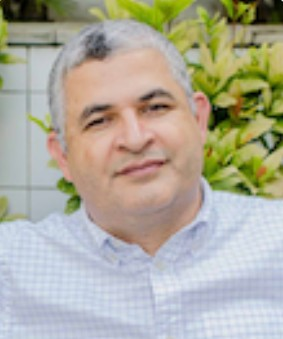
\includegraphics[width=1.45833in,height=1.45833in]{figuras/jjesus.jpg}

Cientista de dados e especialista em jurimetria, atua no desenvolvimento
de ferramentas em R para extração e organização de dados judiciais e na
aplicação de métodos estatísticos ao contencioso. É autor do pacote tjsp
(R) para coleta e organização de processos e decisões do TJSP, com
documentação pública e citação formal do projeto; também ministra cursos
e publica tutoriais práticos sobre raspagem, estruturação e análise de
dados judiciais (tempo de processo, análises de sobrevivência, etc.).
Além do trabalho técnico, participa de eventos da Associação Brasileira
de Jurimetria (ABJ) apresentando aplicações de aprendizado estatístico,
PLN e sistemas distribuídos em dados judiciais .\\
📘 \href{https://lattes.cnpq.br/YYYYYYYYY}{Currículo Lattes} •

🔗 \href{https://linkedin.com/in/XXXX}{LinkedIn}

\bookmarksetup{startatroot}

\chapter{Sumário do Curso ESMAT}\label{sumuxe1rio-do-curso-esmat}

Esta é a página de apoio do Professor Alexandre Nicolella e Jose de
Jesus Filho ao curso de Curso de Extensão em Jurimetria da Escola
Superior da Magistratura Tocantinense (ESMAT).

\section{\texorpdfstring{\textbf{Motivação}:}{Motivação:}}\label{motivauxe7uxe3o-1}

O curso tem como propósito introduzir os participantes aos conceitos
fundamentais de jurimetria e de inteligência artificial aplicada ao
Direito, oferecendo uma formação integrada entre teoria e prática. A
proposta parte da compreensão de como métodos quantitativos e
computacionais podem apoiar a análise jurídica, aprimorando a tomada de
decisão e promovendo maior eficiência e transparência no sistema de
Justiça.

A motivação central é capacitar os alunos a desenvolver uma visão
empírica do Direito, a partir de atividades que envolvem o desenho de
pesquisa e a definição de hipóteses, o planejamento de estratégias de
coleta e listagem de processos, e a estruturação, limpeza e organização
de bases de dados jurídicas.

Durante o curso, serão exploradas ferramentas e pacotes da linguagem R
voltados à manipulação e à visualização de dados jurídicos, com
aplicação prática em exemplos reais do Tribunal de Justiça do Tocantins
(TJTO). A combinação entre conceitos teóricos, prática orientada por
problemas e uso de dados reais visa proporcionar uma formação sólida e
aplicada, aproximando os participantes dos desafios contemporâneos da
jurimetria e da análise de dados no Direito.

\section{\texorpdfstring{\textbf{Objetivo}:}{Objetivo:}}\label{objetivo-1}

O objetivo é fornecer aos participantes competências necessárias para: -
Formular e estruturar pesquisas empíricas no Direito. - Extrair e
organizar dados processuais de forma sistemática. - Aplicar ferramentas
estatísticas e computacionais básicas para análise inicial de dados
jurídicos. - Criar visualizações que traduzam informações complexas em
resultados claros e objetivos.

\section{\texorpdfstring{\textbf{Professores}}{Professores}}\label{professores}

Os professores do curso são:

\begin{longtable}[]{@{}ll@{}}
\toprule\noalign{}
Professor & Email \\
\midrule\noalign{}
\endhead
\bottomrule\noalign{}
\endlastfoot
Alexandre Chibebe Nicolella & nicolella@usp.br \\
José de Jesus Filho & jose.filho@mpsp.mp.br; jjfilho@pucsp.br \\
\end{longtable}

\bookmarksetup{startatroot}

\chapter{O Cronograma das Aulas:}\label{o-cronograma-das-aulas}

\section{Etapa Online: Fundamentos e Conceitos (6 horas
síncronas)}\label{etapa-online-fundamentos-e-conceitos-6-horas-suxedncronas}

Nesta fase, os participantes terão contato com os \textbf{conceitos
fundamentais de jurimetria} e \textbf{inteligência artificial aplicada
ao Direito}. O enfoque será teórico, preparando o terreno para a etapa
prática.

\subsection{Aula 01 - Introdução ao Desenho de Pesquisa e à
Jurimetria}\label{aula-01---introduuxe7uxe3o-ao-desenho-de-pesquisa-e-uxe0-jurimetria}

\begin{itemize}
\tightlist
\item
  Conceito de jurimetria e a interdisciplinaridade necessária (Direito,
  Computação e Estatística)\\
\item
  Jurimetria e inteligência artificial aplicada ao Direito\\
\item
  Exemplos práticos de jurimetria
\item
  Pergunta de pesquisa\\
\item
  Formulação da hipótese\\
\item
  Operacionalização de conceitos\\
\item
  Inferência causal
\end{itemize}

\subsection{Aula 02 - Análise de Viabilidade e Listagem de
Processos}\label{aula-02---anuxe1lise-de-viabilidade-e-listagem-de-processos}

\begin{itemize}
\tightlist
\item
  Análise de viabilidade\\
\item
  Escopo de pesquisa: pesquisa prospectiva vs.~retrospectiva (resultado,
  tempo e distribuição)\\
\item
  Sistemas de listagem (CJ e CPO)\\
\item
  Introdução ao pacote \texttt{tjsp}
\end{itemize}

\section{Etapa Presencial: Aplicação Prática no Tocantins (24
horas)}\label{etapa-presencial-aplicauxe7uxe3o-pruxe1tica-no-tocantins-24-horas}

Realizada no Tocantins, esta etapa é dividida em duas partes. Na
primeira, os participantes terão noções de ciência de dados para
coletar, organizar, estruturar e analisar dados de processos judiciais,
com duração de um dia de oito horas.

\subsection{Aula 03 - Estruturação de Dados
I}\label{aula-03---estruturauxe7uxe3o-de-dados-i}

\begin{itemize}
\tightlist
\item
  Introdução ao \texttt{dplyr}\\
\item
  Tratamento de datas com \texttt{lubridate}\\
\item
  Tratamento de texto com \texttt{stringr}\\
\item
  Iteração com \texttt{purrr}
\end{itemize}

\subsection{Aula 04 - Estruturação de Dados
II}\label{aula-04---estruturauxe7uxe3o-de-dados-ii}

\begin{itemize}
\tightlist
\item
  Introdução aos Large Language Models (LLMs)\\
\item
  Engenharia de prompt
\end{itemize}

\subsection{Aula 05 - Visualização de
Dados}\label{aula-05---visualizauxe7uxe3o-de-dados}

\begin{itemize}
\tightlist
\item
  Noções básicas de estatística\\
\item
  Introdução ao \texttt{ggplot2}
\end{itemize}

A segunda fase, com duração de 16 horas, divididas em dois dias, será
totalmente prática e orientada a resultados. Os participantes serão
organizados em grupos de trabalho por tema, e cada grupo desenvolverá um
projeto jurimétrico completo, percorrendo as seguintes etapas:

\begin{enumerate}
\def\labelenumi{\arabic{enumi}.}
\tightlist
\item
  Definição de uma pergunta de pesquisa aplicada ao contexto do TJTO.\\
\item
  Coleta de dados judiciais relevantes.\\
\item
  Estruturação, organização e limpeza das bases.\\
\item
  Análise exploratória e visualização de resultados.\\
\item
  Apresentação final dos achados.
\end{enumerate}

Ao final do módulo, os participantes terão vivenciado o \textbf{ciclo
completo da jurimetria}, desde a formulação inicial até a comunicação
dos resultados, combinando competências jurídicas, estatísticas e
computacionais.

\section{Método de Trabalho}\label{muxe9todo-de-trabalho}

\subsection{Divisão do Curso em Módulos e
Formatos}\label{divisuxe3o-do-curso-em-muxf3dulos-e-formatos}

\textbf{Online (6h, síncrono):} - Desenvolvimento dos conceitos centrais
de forma teórica\\
- Discussão de fundamentos, referências e boas práticas\\
- Interação por meio de exercícios guiados e debates curtos

\textbf{Presencial (8h, em Tocantins) - PARTE I:} - Estruturação de
dados\\
- Análise Estatística Descritiva\\
- Visulaização

\textbf{Presencial (24h, em Tocantins) - PARTE II:}

\begin{enumerate}
\def\labelenumi{\arabic{enumi}.}
\tightlist
\item
  \textbf{Definição do problema ou pergunta de pesquisa:} cada grupo
  escolhe um tema específico a partir dos conceitos apresentados.\\
\item
  \textbf{Coleta e organização de dados/informações:} orientação sobre
  como levantar dados relevantes para a análise.\\
\item
  \textbf{Análise e interpretação dos resultados:} uso das ferramentas e
  métodos aprendidos na parte online.\\
\item
  \textbf{Apresentação e discussão dos resultados:} compartilhamento das
  conclusões e lições aprendidas.
\end{enumerate}

\subsection{Integração Teoria e
Prática}\label{integrauxe7uxe3o-teoria-e-pruxe1tica}

O método garante que os conceitos vistos online e presencialmente sejam
aplicados de forma concreta.\\
A interação presencial reforça o aprendizado ativo e colaborativo.

\subsection{Feedback e Aprimoramento}\label{feedback-e-aprimoramento}

\begin{itemize}
\tightlist
\item
  Avaliação contínua do progresso dos grupos.\\
\item
  Discussões coletivas para melhorar abordagens e resultados.
\end{itemize}

\section{Infraestrutura e Dados}\label{infraestrutura-e-dados}

\subsection{Dados}\label{dados}

Os dados utilizados no curso serão fornecidos pelo \textbf{TJTO},
diretamente ou via uso de \textbf{API} para acesso à informação.

\subsection{Computadores e Rede}\label{computadores-e-rede}

\begin{itemize}
\tightlist
\item
  Cada participante terá acesso a um computador individual.\\
\item
  Todos os computadores estarão conectados à internet de alta
  velocidade.
\end{itemize}

\subsection{Softwares e Ferramentas}\label{softwares-e-ferramentas}

\begin{itemize}
\tightlist
\item
  \textbf{R} (versão mais recente) pré-instalado em todas as máquinas.\\
\item
  Instalação de \emph{packages} adicionais conforme necessidade dos
  exercícios.\\
\item
  Outros softwares de apoio poderão ser instalados mediante solicitação.
\end{itemize}

\subsection{Ambiente de Trabalho}\label{ambiente-de-trabalho}

\begin{itemize}
\tightlist
\item
  Espaço preparado para trabalho em grupo e colaboração.\\
\item
  Projetor e quadro branco disponíveis.\\
\item
  Suporte técnico para instalação de pacotes e resolução de problemas.
\end{itemize}

\subsection{Segurança e Backup}\label{seguranuxe7a-e-backup}

\begin{itemize}
\tightlist
\item
  Sistemas de backup configurados para evitar perda de dados.\\
\item
  Garantia de que os participantes possam salvar e recuperar seus
  projetos com segurança.
\end{itemize}

\section{Resultados Esperados}\label{resultados-esperados}

\subsection{Aprendizado Conceitual}\label{aprendizado-conceitual}

\begin{itemize}
\tightlist
\item
  Compreensão dos fundamentos, metodologias e boas práticas do tema.\\
\item
  Capacidade de aplicar conceitos teóricos em situações reais.
\end{itemize}

\subsection{Habilidades Práticas}\label{habilidades-pruxe1ticas}

\begin{itemize}
\tightlist
\item
  Desenvolvimento da análise de dados e interpretação de resultados
  utilizando R.\\
\item
  Experiência em trabalho colaborativo, da definição do problema à
  apresentação de soluções.
\end{itemize}

\subsection{Produção de Resultados
Concretos}\label{produuxe7uxe3o-de-resultados-concretos}

\begin{itemize}
\tightlist
\item
  Cada grupo produzirá relatórios ou apresentações com análise detalhada
  de seu tema.\\
\item
  Discussão coletiva dos resultados, promovendo aprendizado entre todos.
\end{itemize}

\subsection{Fortalecimento da Capacidade
Analítica}\label{fortalecimento-da-capacidade-analuxedtica}

\begin{itemize}
\tightlist
\item
  Habilidade de formular perguntas relevantes, organizar dados, aplicar
  métodos e tirar conclusões consistentes.\\
\item
  Preparação para aplicar o conhecimento em projetos profissionais ou
  acadêmicos.
\end{itemize}

\subsection{Feedback e Melhoria
Contínua}\label{feedback-e-melhoria-contuxednua}

\begin{itemize}
\tightlist
\item
  Feedback detalhado sobre os trabalhos dos grupos.\\
\item
  Incentivo à reflexão sobre processos e resultados, promovendo
  aprimoramento contínuo.
\end{itemize}

\section{Bibliografia}\label{bibliografia}

AGRESTI, Alan; FINLAY, Barbara. \emph{Métodos Estatísticos para as
Ciências Sociais.} São Paulo: Tenso, 2017.\\
AMINIKHANGHAHI, Samaneh; COOK, Daniel J. \emph{A Survey of Methods for
Time Series Change Point Detection.} \emph{Knowl Inf Syst}, v. 51,
p.~339--367, 2017. DOI: 10.1007/s10115-016-0987-z.\\
ENDERS, Craig. \emph{Applied Missing Data Analysis.} New York: The
Guilford Press, 2022.\\
EPSTEIN, Lee; KING, Gary. \emph{As Regras de Inferência.} São Paulo:
Direito GV, 2013.\\
GALANTER, Marc. \emph{Why the `Haves' Come Out Ahead: Speculations on
the Limit of Social Change.} \emph{Law and Society Review}, v. 9:1,
1974.\\
HILBE, Joseph. \emph{Practical Guide for Logistic Regression.} Chapman
and Hall/CRC, 2018.\\
KELLSTEDT, Paul M.; WHITTEN, Guy D. \emph{Fundamentos da Pesquisa em
Ciência Política.} São Paulo: Blucher, 2014.\\
KING, Gary; KEOHANE, Roberto; VERBA, Sidney. \emph{Designing Social
Inquiry: Scientific Inference for Qualitative Methods.} 2021.\\
LEE, Alex Yoon-Ho; KLERMAN, Daniel M. \emph{The Priest-Klein Hypotheses:
Proofs and Generality.} \emph{International Review of Law and
Economics}, v. 59, 2016.\\
MOORE, Dirk F. \emph{Applied Survival Analysis Using R.} Switzerland:
Springer, 2016.\\
MORETTIN, Wilton de O.; BUSSAB, Pedro A. \emph{Estatística Básica.} São
Paulo: Saraiva, 2021.\\
PRIEST, George L.; KLEIN, Benjamin. \emph{The Selection of Disputes for
Litigation.} \emph{Journal of Legal Studies}, v. XIII, jan. 1984.\\
SILVA, Glauco. \emph{Desenho de Pesquisa.} São Paulo: ENAP, 2018.\\
STOCK, James H.; WATSON, Mark W. \emph{Introduction to Econometrics.}
London: Pearson, 2020.\\
WOOLDRIDGE, Jeffrey M. \emph{Introductory Econometrics: A Modern
Approach.} South Western Educational Publishing, 2012.\\
KILLICK, Rebecca; ECKLEY, Idris A. \emph{changepoint: An R Package for
Changepoint Analysis.} \emph{Journal of Statistical Software}, 58(3),
1--19, 2014. DOI:
\href{https://doi.org/10.18637/jss.v058.i03}{10.18637/jss.v058.i03}.\\
TOOMET, Ott; HENNINGSEN, Arne. \emph{Sample Selection Models in R:
Package sampleSelection.} \emph{Journal of Statistical Software}, 27(7),
1--23, 2008. DOI:
\href{https://doi.org/10.18637/jss.v027.i07}{10.18637/jss.v027.i07}.\\
TRUONGA, Charles; OUDRE, Laurent; VAYATIS, Nicolas. \emph{Selective
Review of Offline Change Point Detection Methods.} \emph{Signal
Processing}, 167, 2020.

\bookmarksetup{startatroot}

\chapter{Maipulando os Dados}\label{maipulando-os-dados}

Uma Breve Introdução ao R

\hfill\break

\section{O R-project e as Boas
Práticas}\label{o-r-project-e-as-boas-pruxe1ticas}

\subsection{O software R}\label{o-software-r}

O R é uma linguagem e ambiente de desenvolvimento de Estatística e
gráficos. É uma ferramenta poderosa, fornecendo ao seu usuário maior
integração e qualidade gráfica e de análise. Alguns motivos para
utilizar o R:

\begin{itemize}
\item
  \textbf{É Gratuito}: é um projeto open-source. Pode ser utilizado em
  qualquer sistema operacional e tem aberto seus códigos e pactos para
  poder ser inspecionado.
\item
  \textbf{R é uma Linguagem}:Requer que seja escrito um script ao invés
  de clicar. A primeira vista uma característica negativa, entretanto,
  permite maior exploração, organização, memória da atividade, maior
  integração entre processos etc.
\item
  \textbf{Gráficos e Visualizações}: É sem sombra de dúvida o pacote
  estatístico com melhor e mais poderosa ferramenta de elaboração de
  gráficos e visualização.
\item
  \textbf{Pacotes Estatísticos}:Já possui muitas rotinas de análises já
  programadas nos diversos pacotes desenvolvidos, sendo muito bem
  documentados. Já possui muitas rotinas para regressão, regressão com
  séries temporais, regressão em painel, finanças, modelos de
  causalidade etc.
\item
  \textbf{Fronteira do Conhecimento}: Os principais desenvolvimentos
  teóricos em Econometria tem sua aplicação demonstrada e desenvolvida
  utilizando o R. Isso é valido para todas as subáreas do conhecimento
  em econometria, séries temporais, painel, finanças, etc.
\item
  \textbf{Recursos de Ajuda}: Há uma comunidade muito grande disponível
  para solucionar dúvidas e uma vasta documentação disponível para
  consulta na rede.
\item
  \textbf{Conexão com Outros Pacotes}: O R integra com outros pacotes
  que automatizam o nosso trabalho cotidiano. Pode se conectar com o
  Python, Java, SQL, Latex etc.
\end{itemize}

\subsection{Utilizando Interface Gráfica - O
Rstudio}\label{utilizando-interface-gruxe1fica---o-rstudio}

Pode-se realizar seu script diretamente no console do R. Ele irá
realizar um comando por vez. O R é uma interface leve e com poucos
recursos gráficos.

Uma alternativa ao uso do R diretamente é o Rstudio, o qual é um editor
de código ou um ambiente de desenvolvimento integrado. Ele possui quatro
janelas, sendo a primeira a janela de script (superior esquerda) onde
escrevemos os comandos em R.

A segunda janela é o console (inferior esquerda) similar ao que temos no
R e onde os resultados são apresentados. Pode-se digitar comando
diretamente no console do RStudio.

A terceira é a janela de ambiente e história (superior direita) ela
armazena seus dados, valores e funções e a aba história possui a memoria
dos comandos realizados.

Por fim a quarta janela (inferior direita) apresenta os pacotes, os
gráficos, os arquivos gerados e ajuda. Essa janela facilita a instalação
de pacotes, carregamento de bibliotecas, visualização de gráficos e o
caminho dos arquivos.

\subsection{Ajuda}\label{ajuda}

Para abrir a ajuda geral o seguinte abaixo pode ser utilizado e abrirá
uma janela no seu navegador.

\begin{Shaded}
\begin{Highlighting}[]
\FunctionTok{help.start}\NormalTok{()}
\end{Highlighting}
\end{Shaded}

Suponha que queiramos saber de uma função específica, assim pode-se
utilizar o seguinte comando:

\begin{Shaded}
\begin{Highlighting}[]
\FunctionTok{help}\NormalTok{(summary)}
\end{Highlighting}
\end{Shaded}

ou

\begin{Shaded}
\begin{Highlighting}[]
\NormalTok{?summary}
\end{Highlighting}
\end{Shaded}

Inclusive pode pedir um exemplo de como utilizar a função que está
buscando

\begin{Shaded}
\begin{Highlighting}[]
\FunctionTok{example}\NormalTok{(summary)}
\end{Highlighting}
\end{Shaded}

\subsection{Boas Práticas}\label{boas-pruxe1ticas}

É fundamental que o usuário seja organizado. Forma é muito importante!
Assim o usuário deve adotar padrões que auxiliem na organização do seu
script ou programa.

\textbf{Case Sensitivy}: O R diferencia letras minúsculas e maiúscula.
Ou seja, m é diferente de M. Por exemplo, considere as três formas de
escrever a palavra idade.

\textbf{idade} ou \textbf{Idade} ou \textbf{IDADE}

Cada uma delas representa variáveis diferentes.

\begin{tcolorbox}[enhanced jigsaw, leftrule=.75mm, coltitle=black, colframe=quarto-callout-tip-color-frame, toprule=.15mm, opacitybacktitle=0.6, bottomtitle=1mm, bottomrule=.15mm, titlerule=0mm, toptitle=1mm, title=\textcolor{quarto-callout-tip-color}{\faLightbulb}\hspace{0.5em}{DICA}, arc=.35mm, breakable, opacityback=0, colbacktitle=quarto-callout-tip-color!10!white, colback=white, left=2mm, rightrule=.15mm]

Sempre utilize as suas variáveis em minúsculo. Adote isso como regra
geral.

\end{tcolorbox}

\textbf{Criando Bons Nomes}: Vamos supor que queiramos criar uma
variável que indique a idade que se formou na Universidade. Temos
algumas opções:

\begin{itemize}
\tightlist
\item
  \textbf{id}: Ruim, pois não tem significado claro e pode confundir com
  a variável de identificação
\item
  \textbf{idade\_formou\_na\_universidade}: Ruim, pois o nome da
  variável é muito grande, difícil de escrever e de visualizar no banco
  de dados.
\item
  \textbf{idade\_form}: Bom nome, significativo, minúsculo e pequeno
  separa os dois nomes por underline
\item
  \textbf{idadeForm} :Bom nome, significativo, minúsculo e pequeno
  separa os dois nomes por uma letra maiúscula.
\end{itemize}

\begin{tcolorbox}[enhanced jigsaw, leftrule=.75mm, coltitle=black, colframe=quarto-callout-tip-color-frame, toprule=.15mm, opacitybacktitle=0.6, bottomtitle=1mm, bottomrule=.15mm, titlerule=0mm, toptitle=1mm, title=\textcolor{quarto-callout-tip-color}{\faLightbulb}\hspace{0.5em}{DICA}, arc=.35mm, breakable, opacityback=0, colbacktitle=quarto-callout-tip-color!10!white, colback=white, left=2mm, rightrule=.15mm]

Adote uma regra de criação para você e evite mudar. Crie nomes pequenos
e significativos. Nunca inicie uma variável com número.

\end{tcolorbox}

\subsection{Criando projeto no R}\label{criando-projeto-no-r}

Para saber em qual diretório o R está utilizando para salvar seu espaço
de trabalho utilize o seguinte comando:

\begin{Shaded}
\begin{Highlighting}[]
\FunctionTok{getwd}\NormalTok{() }
\end{Highlighting}
\end{Shaded}

No RStudio, sempre prefira a criação de um projeto para a organização de
seus dados, com isso, ao mudar de máquina (ou estrutura de diretórios)
seu código continuará funcionando normalmente.

\begin{Shaded}
\begin{Highlighting}[]
\NormalTok{  File }\OtherTok{{-}\textgreater{}}\NormalTok{ New Project}
\end{Highlighting}
\end{Shaded}

\subsection{Identação é
Importante}\label{identauxe7uxe3o-uxe9-importante}

Identar é o recuo no texto em relação a margem. É importante que esse
recuo exista para linhas do seu programa que são hierarquicamente
conectadas. Vejamos dois exemplos com e sem identação:

\emph{Sem Identação}

\begin{Shaded}
\begin{Highlighting}[]
\NormalTok{x}\OtherTok{=}\FunctionTok{c}\NormalTok{()}
\NormalTok{x[}\DecValTok{1}\NormalTok{] }\OtherTok{=} \DecValTok{3}
\ControlFlowTok{for}\NormalTok{ (i }\ControlFlowTok{in} \DecValTok{2}\SpecialCharTok{:}\DecValTok{9}\NormalTok{) \{ }
\NormalTok{x[i]}\OtherTok{=}\DecValTok{2}\SpecialCharTok{*}\NormalTok{x[i}\DecValTok{{-}1}\NormalTok{]}
\NormalTok{\}}
\end{Highlighting}
\end{Shaded}

Note que a quarta linha desse programa está hierarquicamente conectada a
linha 3 do ``for'', ou seja, é uma continuação do comando e portanto
deve ser identado para demonstrar essa relação de dependência. Vejamos

\emph{Com Identação}

\begin{Shaded}
\begin{Highlighting}[]
\NormalTok{x}\OtherTok{=}\FunctionTok{c}\NormalTok{()}
\NormalTok{x[}\DecValTok{1}\NormalTok{] }\OtherTok{=} \DecValTok{3}
\ControlFlowTok{for}\NormalTok{ (i }\ControlFlowTok{in} \DecValTok{2}\SpecialCharTok{:}\DecValTok{9}\NormalTok{) \{ }
\NormalTok{  x[i]}\OtherTok{=}\DecValTok{2}\SpecialCharTok{*}\NormalTok{x[i}\DecValTok{{-}1}\NormalTok{]}
\NormalTok{\}}
\end{Highlighting}
\end{Shaded}

\section{Inserindo Dados no R}\label{inserindo-dados-no-r}

\subsection{Tipos de Variáveis}\label{tipos-de-variuxe1veis}

O R possui diversos tipos de variáveis. Alguns desses tipos são:

\textbf{Vetores}: Vamos inserir os dados denúmero de homicídios de
mulheres nos diversos Estados brasileiros para o ano de 2022.No primeiro
elemento teremos um erro, ao invés de 22 colocaremos 2.E não colocamos o
valor do Distrito Federal e nem Tocantins

\begin{Shaded}
\begin{Highlighting}[]
\NormalTok{homic }\OtherTok{\textless{}{-}} \FunctionTok{c}\NormalTok{(}\DecValTok{2}\NormalTok{,  }\DecValTok{73}\NormalTok{,  }\DecValTok{22}\NormalTok{,  }\DecValTok{88}\NormalTok{,  }\DecValTok{406}\NormalTok{,  }\DecValTok{264}\NormalTok{,    }\DecValTok{95}\NormalTok{,  }\DecValTok{137}\NormalTok{,  }\DecValTok{127}\NormalTok{,  }\DecValTok{101}\NormalTok{,  }\DecValTok{75}\NormalTok{,  }\DecValTok{309}\NormalTok{,  }\DecValTok{200}\NormalTok{,  }\DecValTok{86}\NormalTok{,  }\DecValTok{256}\NormalTok{,  }\DecValTok{219}\NormalTok{,  }\DecValTok{70}\NormalTok{,  }\DecValTok{283}\NormalTok{,  }\DecValTok{60}\NormalTok{,  }\DecValTok{281}\NormalTok{,  }\DecValTok{88}\NormalTok{,  }\DecValTok{33}\NormalTok{,  }\DecValTok{101}\NormalTok{,  }\DecValTok{423}\NormalTok{,  }\DecValTok{37}\NormalTok{)}
\NormalTok{homic}
\end{Highlighting}
\end{Shaded}

\begin{verbatim}
 [1]   2  73  22  88 406 264  95 137 127 101  75 309 200  86 256 219  70 283  60
[20] 281  88  33 101 423  37
\end{verbatim}

Podemos inserir vetores de texto, por exemplo, iremos inserir os estados
brasileiros na mesma ordem do homicídio acima.

\begin{verbatim}
 [1] "Acre"                "Alagoas"             "Amapá"              
 [4] "Amazonas"            "Bahia"               "Ceará"              
 [7] "Distrito Federal "   "Espírito Santo"      "Goiás"              
[10] "Maranhão"            "Mato Grosso"         "Mato Grosso do Sul" 
[13] "Minas Gerais"        "Pará"                "Paraíba"            
[16] "Paraná"              "Pernambuco"          "Piauí"              
[19] "Rio de Janeiro"      "Rio Grande do Norte" "Rio Grande do Sul"  
[22] "Rondônia"            "Roraima"             "Santa Catarina"     
[25] "São Paulo"           "Sergipe"             "Tocantins"          
\end{verbatim}

Algumas manipulações importantes que podemos fazer com os vetores.
Renomeando e removendo o vetor antigo:

Trocando o primeiro elemento do vetor e dando o print do novo resultado:

\begin{Shaded}
\begin{Highlighting}[]
\NormalTok{homic\_abs[}\DecValTok{1}\NormalTok{]}\OtherTok{=}\DecValTok{22}
\NormalTok{homic\_abs}
\end{Highlighting}
\end{Shaded}

\begin{verbatim}
 [1]  22  73  22  88 406 264  95 137 127 101  75 309 200  86 256 219  70 283  60
[20] 281  88  33 101 423  37
\end{verbatim}

Algumas maneiras de pedir o print do vetor de homicídios femininos.
Somente o estado 7, todos menos o estado 7, Estado de 1 até 7 etc:

\begin{Shaded}
\begin{Highlighting}[]
\NormalTok{homic\_abs[}\DecValTok{7}\NormalTok{] }
\end{Highlighting}
\end{Shaded}

\begin{verbatim}
[1] 95
\end{verbatim}

\begin{Shaded}
\begin{Highlighting}[]
\NormalTok{homic\_abs[}\SpecialCharTok{{-}}\DecValTok{7}\NormalTok{] }
\end{Highlighting}
\end{Shaded}

\begin{verbatim}
 [1]  22  73  22  88 406 264 137 127 101  75 309 200  86 256 219  70 283  60 281
[20]  88  33 101 423  37
\end{verbatim}

\begin{Shaded}
\begin{Highlighting}[]
\NormalTok{homic\_abs[}\DecValTok{1}\SpecialCharTok{:}\DecValTok{7}\NormalTok{]}
\end{Highlighting}
\end{Shaded}

\begin{verbatim}
[1]  22  73  22  88 406 264  95
\end{verbatim}

Podemos incorporar novos dados no nosso vetor de homicídio feminino,
Vamos incorporar o dado do Tocantins na posição 7 e o valor do Distrito
Federal na útima posição - 27. Depois trocaremos os dois estados de
posição:

\begin{Shaded}
\begin{Highlighting}[]
\CommentTok{\#colcar exemplo de inserir no inicio}

\CommentTok{\#inserir no meio e no final }
\NormalTok{homic\_abs }\OtherTok{\textless{}{-}} \FunctionTok{c}\NormalTok{(homic\_abs[}\DecValTok{1}\SpecialCharTok{:}\DecValTok{6}\NormalTok{], }\DecValTok{36}\NormalTok{,homic\_abs[}\DecValTok{7}\SpecialCharTok{:}\DecValTok{25}\NormalTok{], }\DecValTok{32}\NormalTok{)}
\NormalTok{homic\_abs}
\end{Highlighting}
\end{Shaded}

\begin{verbatim}
 [1]  22  73  22  88 406 264  36  95 137 127 101  75 309 200  86 256 219  70 283
[20]  60 281  88  33 101 423  37  32
\end{verbatim}

\begin{Shaded}
\begin{Highlighting}[]
\CommentTok{\#troca de posicoes}
\NormalTok{temp }\OtherTok{\textless{}{-}}\NormalTok{ homic\_abs[}\DecValTok{27}\NormalTok{]}
\NormalTok{homic\_abs[}\DecValTok{27}\NormalTok{] }\OtherTok{\textless{}{-}}\NormalTok{ homic\_abs[}\DecValTok{7}\NormalTok{]}
\NormalTok{homic\_abs[}\DecValTok{7}\NormalTok{] }\OtherTok{\textless{}{-}}\NormalTok{ temp}
\NormalTok{homic\_abs}
\end{Highlighting}
\end{Shaded}

\begin{verbatim}
 [1]  22  73  22  88 406 264  32  95 137 127 101  75 309 200  86 256 219  70 283
[20]  60 281  88  33 101 423  37  36
\end{verbatim}

\textbf{String ou Texto}:

String são as variáveis tipo texto. Esse tipo de variável já apareceu na
seção anterior quando apresentamos um vetor com a classificação dos
Estados. Vejamos mais uma vez. Podemos criar uma variável que contêm
``estado homicidio''. Uma segunda maneira é criar um vetor com dois
elementos ``estado'' e ``homicidio''. O comando \texttt{paste} cola a
variável texto ``estado'' e a variável texto ``homicidio'', separado por
um espaço.

\begin{Shaded}
\begin{Highlighting}[]
\NormalTok{a }\OtherTok{\textless{}{-}} \StringTok{"estado homicidio"}
\NormalTok{a}
\end{Highlighting}
\end{Shaded}

\begin{verbatim}
[1] "estado homicidio"
\end{verbatim}

\begin{Shaded}
\begin{Highlighting}[]
\NormalTok{b }\OtherTok{\textless{}{-}} \FunctionTok{c}\NormalTok{(}\StringTok{"estado"}\NormalTok{,}\StringTok{"homicidio"}\NormalTok{)}
\NormalTok{b}
\end{Highlighting}
\end{Shaded}

\begin{verbatim}
[1] "estado"    "homicidio"
\end{verbatim}

\begin{Shaded}
\begin{Highlighting}[]
\NormalTok{b[}\DecValTok{1}\NormalTok{]}
\end{Highlighting}
\end{Shaded}

\begin{verbatim}
[1] "estado"
\end{verbatim}

\begin{Shaded}
\begin{Highlighting}[]
\FunctionTok{paste}\NormalTok{(b[}\DecValTok{1}\NormalTok{],b[}\DecValTok{2}\NormalTok{],}\AttributeTok{sep=}\StringTok{\textquotesingle{} \textquotesingle{}}\NormalTok{)}
\end{Highlighting}
\end{Shaded}

\begin{verbatim}
[1] "estado homicidio"
\end{verbatim}

\textbf{Fator}:

Fator são variáveis de classe. Fator armazenam os valores inteiros na
forma de um vetor com as quantidades das k classes e o vetor string dos
valores originais. Vejamos o exemplo de um vetor. Podemos análisar os
homicídios por região geográfica do país. Assim, classificaremos os
estados por região:

\begin{Shaded}
\begin{Highlighting}[]
\NormalTok{regiao }\OtherTok{\textless{}{-}} \FunctionTok{c}\NormalTok{(}\StringTok{"N"}\NormalTok{,  }\StringTok{"NE"}\NormalTok{,  }\StringTok{"N"}\NormalTok{,  }\StringTok{"N"}\NormalTok{,  }\StringTok{"NE"}\NormalTok{,  }\StringTok{"NE"}\NormalTok{,  }\StringTok{"CO"}\NormalTok{,  }\StringTok{"SD"}\NormalTok{,  }\StringTok{"CO"}\NormalTok{,  }\StringTok{"NE"}\NormalTok{,  }\StringTok{"CO"}\NormalTok{,  }\StringTok{"CO"}\NormalTok{,  }\StringTok{"SD"}\NormalTok{,  }\StringTok{"N"}\NormalTok{,  }\StringTok{"NE"}\NormalTok{,  }\StringTok{"S"}\NormalTok{,  }\StringTok{"NE"}\NormalTok{,  }\StringTok{"NE"}\NormalTok{,  }\StringTok{"SD"}\NormalTok{,  }\StringTok{"NE"}\NormalTok{,  }\StringTok{"S"}\NormalTok{,  }\StringTok{"N"}\NormalTok{,  }\StringTok{"N"}\NormalTok{,  }\StringTok{"S"}\NormalTok{,  }\StringTok{"SD"}\NormalTok{,  }\StringTok{"NE"}\NormalTok{,  }\StringTok{"N"}\NormalTok{)}
\FunctionTok{summary}\NormalTok{(regiao)}
\end{Highlighting}
\end{Shaded}

Agora vamos transformar o vetor anterior em um fator

\begin{Shaded}
\begin{Highlighting}[]
\NormalTok{regiao }\OtherTok{\textless{}{-}} \FunctionTok{factor}\NormalTok{(regiao)}
\FunctionTok{summary}\NormalTok{(regiao)}
\end{Highlighting}
\end{Shaded}

\begin{verbatim}
CO  N NE  S SD 
 4  7  9  3  4 
\end{verbatim}

\begin{Shaded}
\begin{Highlighting}[]
\FunctionTok{levels}\NormalTok{(regiao)}
\end{Highlighting}
\end{Shaded}

\begin{verbatim}
[1] "CO" "N"  "NE" "S"  "SD"
\end{verbatim}

O comando \texttt{levels} fornece as classes existentes, no caso acima
temos 5, sendo elas 4, 7, 9, 3 e 4.

Fatores podem ser as características de raça, gênero, status familiar,
status de saúde, qualidade do atendimento etc.

\subsubsection{Data Frame ou Banco de
Dados}\label{data-frame-ou-banco-de-dados}

Esse é um tipo mais geral de variável e consegue lidar na mesma
estrutura com variaveis de tipos distintos como numérica, texto e fator.
Um banco de dados similar aos outros programas estatísticos. Podemos
criar essa variável de forma manual. Nosso banco de dados será composto
por 4 variáveis, a primeira o estado, a segunda a região, a terceira o
número de homicídios femininos e a quarta o número de feminicidios. As
três primeiras já foram incluidas acima e vamos criar somente a quarta.
O comando \texttt{typeof} mostra qual o tipo de variável.

\begin{Shaded}
\begin{Highlighting}[]
\NormalTok{feminic\_abs}\OtherTok{=}\FunctionTok{c}\NormalTok{(}\DecValTok{11}\NormalTok{,  }\DecValTok{31}\NormalTok{,  }\DecValTok{8}\NormalTok{,  }\DecValTok{21}\NormalTok{,  }\DecValTok{107}\NormalTok{,  }\DecValTok{28}\NormalTok{,  }\DecValTok{19}\NormalTok{,  }\DecValTok{33}\NormalTok{,  }\DecValTok{56}\NormalTok{,  }\DecValTok{69}\NormalTok{,  }\DecValTok{47}\NormalTok{,  }\DecValTok{40}\NormalTok{,  }\DecValTok{171}\NormalTok{,  }\DecValTok{49}\NormalTok{,  }\DecValTok{26}\NormalTok{,  }\DecValTok{77}\NormalTok{,  }\DecValTok{72}\NormalTok{,  }\DecValTok{24}\NormalTok{,  }\DecValTok{111}\NormalTok{,  }\DecValTok{16}\NormalTok{,  }\DecValTok{110}\NormalTok{,  }\DecValTok{24}\NormalTok{,  }\DecValTok{3}\NormalTok{,  }\DecValTok{56}\NormalTok{,  }\DecValTok{195}\NormalTok{,  }\DecValTok{19}\NormalTok{,  }\DecValTok{14}\NormalTok{) }
\FunctionTok{typeof}\NormalTok{(feminic\_abs)}
\end{Highlighting}
\end{Shaded}

\begin{verbatim}
[1] "double"
\end{verbatim}

Para criar o banco de dados utilizamos o seguinte comando:

\begin{Shaded}
\begin{Highlighting}[]
\NormalTok{data\_feminic22}\OtherTok{\textless{}{-}}\FunctionTok{data.frame}\NormalTok{(estados, regiao, homic\_abs, feminic\_abs)  }
\end{Highlighting}
\end{Shaded}

Podemos modificar o nome das variáveis com o comando \texttt{names}.
Entretanto, tem que renomear todas

\begin{Shaded}
\begin{Highlighting}[]
\FunctionTok{names}\NormalTok{(data\_feminic22)}\OtherTok{\textless{}{-}}\FunctionTok{c}\NormalTok{(}\StringTok{"estado"}\NormalTok{, }\StringTok{"regioa"}\NormalTok{, }\StringTok{"homic\_abs"}\NormalTok{, }\StringTok{"feminic\_abs"}\NormalTok{) }
\NormalTok{data\_feminic22}
\end{Highlighting}
\end{Shaded}

Ou podemos renomear somente algumas com o comando \texttt{reshape}:

\begin{Shaded}
\begin{Highlighting}[]
\FunctionTok{library}\NormalTok{(reshape)}
\NormalTok{data\_feminic22 }\OtherTok{\textless{}{-}} \FunctionTok{rename}\NormalTok{(data\_feminic22, }\FunctionTok{c}\NormalTok{(}\AttributeTok{estado=}\StringTok{"estados"}\NormalTok{, }\AttributeTok{regioa=}\StringTok{"regiao"}\NormalTok{))}
\NormalTok{data\_feminic22}
\end{Highlighting}
\end{Shaded}

\begin{verbatim}
               estados regiao homic_abs feminic_abs
1                 Acre      N        22          11
2              Alagoas     NE        73          31
3                Amapá      N        22           8
4             Amazonas      N        88          21
5                Bahia     NE       406         107
6                Ceará     NE       264          28
7    Distrito Federal      CO        32          19
8       Espírito Santo     SD        95          33
9                Goiás     CO       137          56
10            Maranhão     NE       127          69
11         Mato Grosso     CO       101          47
12  Mato Grosso do Sul     CO        75          40
13        Minas Gerais     SD       309         171
14                Pará      N       200          49
15             Paraíba     NE        86          26
16              Paraná      S       256          77
17          Pernambuco     NE       219          72
18               Piauí     NE        70          24
19      Rio de Janeiro     SD       283         111
20 Rio Grande do Norte     NE        60          16
21   Rio Grande do Sul      S       281         110
22            Rondônia      N        88          24
23             Roraima      N        33           3
24      Santa Catarina      S       101          56
25           São Paulo     SD       423         195
26             Sergipe     NE        37          19
27           Tocantins      N        36          14
\end{verbatim}

Podemos também listar variáveis do banco de dados, por exemplo, listar
colunas de 1 a 2 ou listar por nome das variáveis, conforme apresentado
abaixo:

\begin{Shaded}
\begin{Highlighting}[]
\NormalTok{data\_feminic22}
\NormalTok{data\_feminic22[,}\DecValTok{2}\SpecialCharTok{:}\DecValTok{3}\NormalTok{]}
\NormalTok{data\_feminic22[}\DecValTok{1}\SpecialCharTok{:}\DecValTok{2}\NormalTok{,}\DecValTok{2}\SpecialCharTok{:}\DecValTok{3}\NormalTok{]}
\NormalTok{data\_feminic22[}\FunctionTok{c}\NormalTok{(}\StringTok{"regiao"}\NormalTok{,}\StringTok{"feminic\_abs"}\NormalTok{)]}
\end{Highlighting}
\end{Shaded}

Entretanto, inserir dados na mão pode ser uma tarefa muito penosa e
existem soluções bem mais simples e rápidas para inserção de dados. Nas
seções seguintes veremos aprenderemos mais funções úteis para lidar com
banco de dados.

\subsubsection{Trabalhando com as
variáveis:}\label{trabalhando-com-as-variuxe1veis}

Vamos retomar duas variáveis \emph{homic\_abs} e \emph{estado} e vamos
manipular essas duas variáveis. Primeiramente vejamos o número de
elementos, estrutura, classe e nome:

\begin{Shaded}
\begin{Highlighting}[]
\FunctionTok{length}\NormalTok{(homic\_abs) }
\end{Highlighting}
\end{Shaded}

\begin{verbatim}
[1] 27
\end{verbatim}

\begin{Shaded}
\begin{Highlighting}[]
\FunctionTok{str}\NormalTok{(homic\_abs)    }
\end{Highlighting}
\end{Shaded}

\begin{verbatim}
 num [1:27] 22 73 22 88 406 264 32 95 137 127 ...
\end{verbatim}

\begin{Shaded}
\begin{Highlighting}[]
\FunctionTok{class}\NormalTok{(homic\_abs)  }
\end{Highlighting}
\end{Shaded}

\begin{verbatim}
[1] "numeric"
\end{verbatim}

\begin{Shaded}
\begin{Highlighting}[]
\FunctionTok{names}\NormalTok{(homic\_abs) }
\end{Highlighting}
\end{Shaded}

\begin{verbatim}
NULL
\end{verbatim}

Podemos combinar as duas variáveis de forma distintas, por exemplo
combinar na forma de um vetor, combinar como coluna ou combinar como
linha, vejamos a diferença:

\begin{Shaded}
\begin{Highlighting}[]
\CommentTok{\#Precisa mudar essa parte de posição está confuso pois falamos de dataframe e aqui de vetor}
\NormalTok{comb1 }\OtherTok{\textless{}{-}} \FunctionTok{c}\NormalTok{(homic\_abs,estados)      }
\NormalTok{comb2}\OtherTok{\textless{}{-}} \FunctionTok{cbind}\NormalTok{(homic\_abs,estados)}
\NormalTok{comb3 }\OtherTok{\textless{}{-}}\FunctionTok{rbind}\NormalTok{(homic\_abs,estados)}
\NormalTok{comb4 }\OtherTok{\textless{}{-}} \FunctionTok{data.frame}\NormalTok{(}
\NormalTok{              homic\_abs,}
\NormalTok{              estados}
\NormalTok{              ,}\AttributeTok{stringsAsFactors =}\NormalTok{ F)}
\NormalTok{comb1}
\NormalTok{comb2 }
\NormalTok{comb3}
\NormalTok{comb4}
\end{Highlighting}
\end{Shaded}

Vejamos quais objetos temos e vamos pedir para visualizar os objetos que
acabamos de criar. Por fim removeremos o vetor comb1.

\begin{Shaded}
\begin{Highlighting}[]
\FunctionTok{ls}\NormalTok{()  }
\NormalTok{comb1}
\NormalTok{comb2}
\NormalTok{comb3}
\FunctionTok{rm}\NormalTok{(comb1)              }
\end{Highlighting}
\end{Shaded}

\subsection{Importando os Dados}\label{importando-os-dados}

Disponibilizamos dois banco de dados, um contendo os homicídios e
feminicídios por estado e outro com as tentativas. Esses arquivos estão
em formato csv (comma separated values).

Para leitura desse arquivo em csv o seguinte comando é necessário
\texttt{read.csv}, indicado que possui cabeçalho e que o separador é
``;''

\begin{Shaded}
\begin{Highlighting}[]
\NormalTok{df\_feminic22}\OtherTok{\textless{}{-}}\FunctionTok{read.csv}\NormalTok{(}\StringTok{"C:/Users/Alexandre\_Nicolella/Aulas/FEA{-}RP/Jurimetria/dados\_feminic.csv"}\NormalTok{, }\AttributeTok{head=}\ConstantTok{TRUE}\NormalTok{,}\AttributeTok{sep=}\StringTok{";"}\NormalTok{)}

\NormalTok{df\_t\_feminic22}\OtherTok{\textless{}{-}}\FunctionTok{read.csv}\NormalTok{(}\StringTok{"C:/Users/Alexandre\_Nicolella/Aulas/FEA{-}RP/Jurimetria/dados\_tent\_feminic.csv"}\NormalTok{, }\AttributeTok{head=}\ConstantTok{TRUE}\NormalTok{,}\AttributeTok{sep=}\StringTok{";"}\NormalTok{)}
\end{Highlighting}
\end{Shaded}

Para leitura de arquivos em Stata terá que utilizar o pacote
\texttt{foreign}, conforme exemplo abaixo:

\begin{Shaded}
\begin{Highlighting}[]
\FunctionTok{library}\NormalTok{(foreign)}
\NormalTok{stata\_feminic }\OtherTok{\textless{}{-}} \FunctionTok{read.dta}\NormalTok{(}\StringTok{"\textasciitilde{}/feminic.dta"}\NormalTok{)}
\end{Highlighting}
\end{Shaded}

Além desses, o R é capaz de trabalhar com SQL, SAS, SPSS, Excel entre
outros.

\begin{tcolorbox}[enhanced jigsaw, leftrule=.75mm, coltitle=black, colframe=quarto-callout-warning-color-frame, toprule=.15mm, opacitybacktitle=0.6, bottomtitle=1mm, bottomrule=.15mm, titlerule=0mm, toptitle=1mm, title=\textcolor{quarto-callout-warning-color}{\faExclamationTriangle}\hspace{0.5em}{Cuidado com o Ponto}, arc=.35mm, breakable, opacityback=0, colbacktitle=quarto-callout-warning-color!10!white, colback=white, left=2mm, rightrule=.15mm]

O R usa o formato americano de separação numérica. Usa ponto ao invés da
vírgula para separar a unidade dos decimais. No Brasil usamos a vírgula.
Isso sempre gera conflito. No seu csv evite usar acentos nas palavras e
use ponto como separados dos decimais e não use separador dos milhares.
Exemplo: 12500.97

\end{tcolorbox}

\subsection{Exportanto os Dados}\label{exportanto-os-dados}

Podemos exportar os dados em diferentes formatos. Alguns exemplos são
csv, texto delimitado, excel, stata. Vejamos em csv:

\begin{Shaded}
\begin{Highlighting}[]
\FunctionTok{write.table}\NormalTok{(df\_feminic22, }\StringTok{"C:/Users/Alexandre\_Nicolella/Aulas/FEA{-}RP/Jurimetria/export\_feminic.csv"}\NormalTok{, }\AttributeTok{sep=}\StringTok{";"}\NormalTok{)}
\end{Highlighting}
\end{Shaded}

Para exportar em Stata utilize os seguintes comandos:

\begin{Shaded}
\begin{Highlighting}[]
\FunctionTok{library}\NormalTok{(foreign)}
\FunctionTok{write.dta}\NormalTok{(df\_feminic22, }\FunctionTok{paste}\NormalTok{(}\FunctionTok{getwd}\NormalTok{(),}\StringTok{"\textasciitilde{}/Banco de dados/export\_feminic.dta"}\NormalTok{,}\AttributeTok{sep=}\StringTok{\textquotesingle{}\textquotesingle{}}\NormalTok{))}
\end{Highlighting}
\end{Shaded}

\subsection{Lidando com Dados Missing}\label{lidando-com-dados-missing}

Não temos informação para as tentativas de feminicidio para os estados
de São Paulo e Mato Grosso. Uma maneira de lidar com valores missing
seria fazer um subconjunto que veremos mais a frente. Agora seguiremos
alguns passos para analisar os valores missing do nosso banco de dados.

Primeiramente, analisamos se há valores missing no banco de dados:

\begin{Shaded}
\begin{Highlighting}[]
\FunctionTok{is.na}\NormalTok{(df\_t\_feminic22)}
\end{Highlighting}
\end{Shaded}

Podemos desconsiderar os valores \emph{missing} da análise de interesse,
vamos fazer a média do dolar sem considerar os valores missing:

\begin{Shaded}
\begin{Highlighting}[]
\FunctionTok{mean}\NormalTok{(df\_t\_feminic22}\SpecialCharTok{$}\NormalTok{t\_feminic\_abs) }
\end{Highlighting}
\end{Shaded}

\begin{verbatim}
[1] NA
\end{verbatim}

\begin{Shaded}
\begin{Highlighting}[]
\FunctionTok{mean}\NormalTok{(df\_t\_feminic22}\SpecialCharTok{$}\NormalTok{t\_feminic\_abs, }\AttributeTok{na.rm=}\ConstantTok{TRUE}\NormalTok{)}
\end{Highlighting}
\end{Shaded}

\begin{verbatim}
[1] 102.52
\end{verbatim}

Podemos criar um novo banco de dados sem os valores missing.

\begin{Shaded}
\begin{Highlighting}[]
\NormalTok{df\_t\_feminic22\_sem\_missing }\OtherTok{\textless{}{-}} \FunctionTok{na.omit}\NormalTok{(df\_t\_feminic22)}
\FunctionTok{mean}\NormalTok{(df\_t\_feminic22\_sem\_missing}\SpecialCharTok{$}\NormalTok{t\_feminic\_abs)}
\end{Highlighting}
\end{Shaded}

\begin{verbatim}
[1] 102.52
\end{verbatim}

\begin{Shaded}
\begin{Highlighting}[]
\FunctionTok{rm}\NormalTok{(df\_t\_feminic22\_sem\_missing)}
\end{Highlighting}
\end{Shaded}

Outra maneira de excluir os valores missing seria a utilização do
comando \texttt{subset} removendo as observações que contenham valor
missing. Isso será explicado em seção a frente.

Pode-se também recodificar uma determinada variável para missing. Muito
comum nas pesquisas do IBGE os valores missing serem identificados por
um número, por exemplo 999999999999. Dessa forma podemos indicar que
esse não é número e sim um valor missing da seguinte maneira:

\begin{Shaded}
\begin{Highlighting}[]
\NormalTok{df\_t\_feminic22}\SpecialCharTok{$}\NormalTok{t\_feminic\_abs[df\_t\_feminic22}\SpecialCharTok{$}\NormalTok{t\_feminic\_abs}\SpecialCharTok{==}\DecValTok{999999}\NormalTok{] }\OtherTok{\textless{}{-}} \ConstantTok{NA}
\end{Highlighting}
\end{Shaded}

Todos os valores que forem 99 serão exluídos e a celula ficará com um
\emph{NA}

\begin{tcolorbox}[enhanced jigsaw, leftrule=.75mm, coltitle=black, colframe=quarto-callout-warning-color-frame, toprule=.15mm, opacitybacktitle=0.6, bottomtitle=1mm, bottomrule=.15mm, titlerule=0mm, toptitle=1mm, title=\textcolor{quarto-callout-warning-color}{\faExclamationTriangle}\hspace{0.5em}{Dados Missing}, arc=.35mm, breakable, opacityback=0, colbacktitle=quarto-callout-warning-color!10!white, colback=white, left=2mm, rightrule=.15mm]

Doois pontos importantes, dados missing não é 0 e nunca devem ser
substituídos por 0. Pois 0 é um valor e missing é que não sabemos. Outro
ponto é que devemos evitar excluir do banco os dados missing, melhor é
fazer as contas retirando apensa do cálculo

\end{tcolorbox}

\section{Operando o Banco de Dados}\label{operando-o-banco-de-dados}

\subsection{Criando uma Nova
Variável}\label{criando-uma-nova-variuxe1vel}

Vamos criar uma variável que seria a soma dos homicídios e feminicídios
no estado. Para criar a variável precisamos dizer primeiro qual o banco
de dados em que queremos criar e qual o nome da variável, conforme
apresentado na expressão abaixo.

\begin{Shaded}
\begin{Highlighting}[]
\FunctionTok{library}\NormalTok{(reshape)}
\NormalTok{df\_feminic22 }\OtherTok{\textless{}{-}} \FunctionTok{rename}\NormalTok{(df\_feminic22, }\FunctionTok{c}\NormalTok{(}\AttributeTok{feminico\_abs=}\StringTok{"feminic\_abs"}\NormalTok{))}


\NormalTok{df\_t\_feminic22}\SpecialCharTok{$}\NormalTok{t\_total\_abs}\OtherTok{\textless{}{-}}\NormalTok{ df\_t\_feminic22}\SpecialCharTok{$}\NormalTok{t\_feminic\_abs }\SpecialCharTok{+}\NormalTok{ df\_t\_feminic22}\SpecialCharTok{$}\NormalTok{t\_homic\_abs}

\NormalTok{df\_feminic22}\SpecialCharTok{$}\NormalTok{total\_abs}\OtherTok{\textless{}{-}}\NormalTok{ df\_feminic22}\SpecialCharTok{$}\NormalTok{feminic\_abs }\SpecialCharTok{+}\NormalTok{ df\_feminic22}\SpecialCharTok{$}\NormalTok{homic\_abs}
\end{Highlighting}
\end{Shaded}

Agora vamos criar uma variável binária que representa como 1 os estados
que possuem a taxa de feminicídio em relação ao total de homicídios
maior que 50\%. Novamente, precisamos indicar o banco de dados e o nome
da variável no banco de dados.

\begin{Shaded}
\begin{Highlighting}[]
\NormalTok{df\_feminic22}\SpecialCharTok{$}\NormalTok{mais\_50[df\_feminic22}\SpecialCharTok{$}\NormalTok{part\_feminic }\SpecialCharTok{\textless{}} \DecValTok{50}\NormalTok{] }\OtherTok{\textless{}{-}} \DecValTok{0}
\NormalTok{df\_feminic22}\SpecialCharTok{$}\NormalTok{mais\_50[df\_feminic22}\SpecialCharTok{$}\NormalTok{part\_feminic }\SpecialCharTok{\textgreater{}=} \DecValTok{50}\NormalTok{] }\OtherTok{\textless{}{-}} \DecValTok{1}

\NormalTok{df\_feminic22}\SpecialCharTok{$}\NormalTok{mais\_50}
\end{Highlighting}
\end{Shaded}

\begin{verbatim}
 [1] 1 0 0 0 0 0 1 0 0 1 0 1 1 0 0 0 0 0 0 0 0 0 0 1 0 1 0
\end{verbatim}

\subsection{Operadores Aritméticos e
Lógicos}\label{operadores-aritmuxe9ticos-e-luxf3gicos}

Utilizando os vetores criados anteriormente:

\begin{Shaded}
\begin{Highlighting}[]
\NormalTok{feminic\_abs}\SpecialCharTok{\textgreater{}}\DecValTok{50}
\end{Highlighting}
\end{Shaded}

\begin{verbatim}
 [1] FALSE FALSE FALSE FALSE  TRUE FALSE FALSE FALSE  TRUE  TRUE FALSE FALSE
[13]  TRUE FALSE FALSE  TRUE  TRUE FALSE  TRUE FALSE  TRUE FALSE FALSE  TRUE
[25]  TRUE FALSE FALSE
\end{verbatim}

\begin{Shaded}
\begin{Highlighting}[]
\NormalTok{feminic\_abs[feminic\_abs}\SpecialCharTok{\textgreater{}}\DecValTok{50}\NormalTok{]}
\end{Highlighting}
\end{Shaded}

\begin{verbatim}
 [1] 107  56  69 171  77  72 111 110  56 195
\end{verbatim}

\begin{Shaded}
\begin{Highlighting}[]
\NormalTok{feminic\_abs[feminic\_abs }\SpecialCharTok{\textless{}} \DecValTok{50} \SpecialCharTok{|}\NormalTok{ feminic\_abs }\SpecialCharTok{\textgreater{}} \DecValTok{100}\NormalTok{]}
\end{Highlighting}
\end{Shaded}

\begin{verbatim}
 [1]  11  31   8  21 107  28  19  33  47  40 171  49  26  24 111  16 110  24   3
[20] 195  19  14
\end{verbatim}

\begin{Shaded}
\begin{Highlighting}[]
\NormalTok{feminic\_abs[feminic\_abs }\SpecialCharTok{\textgreater{}} \DecValTok{50} \SpecialCharTok{\&}\NormalTok{ feminic\_abs }\SpecialCharTok{\textless{}} \DecValTok{100}\NormalTok{]}
\end{Highlighting}
\end{Shaded}

\begin{verbatim}
[1] 56 69 77 72 56
\end{verbatim}

\begin{Shaded}
\begin{Highlighting}[]
\FunctionTok{mean}\NormalTok{(feminic\_abs)}
\end{Highlighting}
\end{Shaded}

\begin{verbatim}
[1] 53.22222
\end{verbatim}

\begin{Shaded}
\begin{Highlighting}[]
\NormalTok{feminic\_M }\OtherTok{\textless{}{-}}\NormalTok{ (feminic\_abs[feminic\_abs}\SpecialCharTok{\textless{}} \DecValTok{100} \SpecialCharTok{\&}\NormalTok{ feminic\_abs }\SpecialCharTok{\textgreater{}} \DecValTok{50}\NormalTok{])}
\NormalTok{feminic\_M}
\end{Highlighting}
\end{Shaded}

\begin{verbatim}
[1] 56 69 77 72 56
\end{verbatim}

A tabela abaixo contém alguns operadaroes lógicos frequentemente
utilizados.

\begin{longtable}[]{@{}cc@{}}
\caption{Operadores Lógicos no R}\tabularnewline
\toprule\noalign{}
Operador & Significado \\
\midrule\noalign{}
\endfirsthead
\toprule\noalign{}
Operador & Significado \\
\midrule\noalign{}
\endhead
\bottomrule\noalign{}
\endlastfoot
\textless{} & Menor que \\
\textless= & Menor igual \\
\textgreater{} & Maior que \\
\textgreater= & Maior igual \\
== & Exatamente igual \\
!= & Diferente \\
!x & Não x \\
x \textbar{} y & x OU y \\
x \& y & x E y \\
\end{longtable}

\section{Algumas Funções
Importantes}\label{algumas-funuxe7uxf5es-importantes}

\subsection{Ordenando os Dados}\label{ordenando-os-dados}

Vamos ordenar os estados dos nossos 2 \emph{data frames} pela
participação do feminicídio no total de homicídios de mulheres.

\begin{Shaded}
\begin{Highlighting}[]
\NormalTok{df\_feminic22\_ord}\OtherTok{\textless{}{-}}\NormalTok{df\_feminic22[}\FunctionTok{order}\NormalTok{(df\_feminic22}\SpecialCharTok{$}\NormalTok{part\_feminic, }\AttributeTok{decreasing =} \ConstantTok{TRUE}\NormalTok{),] }

\NormalTok{df\_t\_feminic22\_ord}\OtherTok{\textless{}{-}}\NormalTok{df\_t\_feminic22[}\FunctionTok{order}\NormalTok{(df\_t\_feminic22}\SpecialCharTok{$}\NormalTok{part\_t\_feminic, }\AttributeTok{decreasing =} \ConstantTok{TRUE}\NormalTok{),] }
\end{Highlighting}
\end{Shaded}

\subsection{Fazendo Merge}\label{fazendo-merge}

Temos dois \emph{data frames} um contendo homicídios e feminicídios e
outro contendo as tentativas. Vamos agora juntar os dois. Para isso os
bancos devem conter uma chave única que identifica cada linha e essa
deve estar presente nos dois bancos. Inclusive devem ter o mesmo nome.No
caso em questão podemos usar o estado como nossa chave que irá conectar
os dois bancos.

\begin{Shaded}
\begin{Highlighting}[]
\NormalTok{df\_final\_feminic\_22 }\OtherTok{\textless{}{-}} \FunctionTok{merge}\NormalTok{(df\_feminic22,df\_t\_feminic22,}\AttributeTok{by=}\StringTok{"sigla"}\NormalTok{,}\AttributeTok{keep.all=}\ConstantTok{TRUE}\NormalTok{)}
\end{Highlighting}
\end{Shaded}

Agora temos um banco único com homicídios e tentativas de homicídios.

\subsection{Agregando}\label{agregando}

Vamos criar um banco de dados que contenha os valores médios das
variáveis. Para isso vamos agregar fazendo a média por região.
Poderíamos utilizar outra função, como a soma, para fazer a agregação:

\begin{Shaded}
\begin{Highlighting}[]
\NormalTok{regiao\_media }\OtherTok{\textless{}{-}}\FunctionTok{aggregate}\NormalTok{(df\_final\_feminic\_22, }\AttributeTok{by=}\FunctionTok{list}\NormalTok{(df\_final\_feminic\_22}\SpecialCharTok{$}\NormalTok{regiao.x), }\AttributeTok{FUN=}\NormalTok{mean, }\AttributeTok{na.rm=}\ConstantTok{TRUE}\NormalTok{)}
\NormalTok{regiao\_media}
\end{Highlighting}
\end{Shaded}

\begin{verbatim}
  Group.1 sigla estado.x regiao.x homic_abs homic_tx feminic_abs feminic_tx
1      CO    NA       NA       NA  86.25000 4.250000    40.50000   2.100000
2       N    NA       NA       NA  69.85714 6.785714    18.57143   1.871429
3      NE    NA       NA       NA 149.11111 4.355556    43.55556   1.422222
4       S    NA       NA       NA 212.66667 4.000000    81.00000   1.600000
5      SD    NA       NA       NA 277.50000 3.300000   127.50000   1.375000
  part_feminic  rendapc total_abs   mais_50 estado.y regiao.y t_homic_abs
1     50.02500 2011.250 126.75000 0.5000000       NA       NA    258.2500
2     30.01429 1175.286  88.42857 0.1428571       NA       NA    161.7143
3     34.36667 1053.222 192.66667 0.2222222       NA       NA    257.7778
4     41.53333 1983.667 293.66667 0.3333333       NA       NA    450.6667
5     43.82500 1842.750 405.00000 0.2500000       NA       NA    455.7500
  t_homic_tx t_feminic_abs t_feminic_tx part_t_feminic t_total_abs
1  13.375000     126.33333     6.500000       32.67667    387.6667
2  24.657143      50.28571     5.285714       26.44286    212.0000
3   9.311111      85.11111     3.044444       25.72444    342.8889
4   8.966667     169.66667     3.500000       25.98667    620.3333
5   8.875000     185.66667     3.000000       26.50000    660.3333
\end{verbatim}

\subsection{Criando Subconjunto}\label{criando-subconjunto}

\textbf{Selecionando Variáveis}:

Podemos estar interessado em manter somente algumas variáveis no nosso
banco de dados, por exemplo, queremos manter estado e a participação do
feminicídio no total. Assim:

\begin{Shaded}
\begin{Highlighting}[]
\NormalTok{var\_sel }\OtherTok{\textless{}{-}} \FunctionTok{c}\NormalTok{(}\StringTok{"sigla"}\NormalTok{, }\StringTok{"part\_feminic"}\NormalTok{, }\StringTok{"part\_t\_feminic"}\NormalTok{)}
\NormalTok{feminic\_sel }\OtherTok{\textless{}{-}}\NormalTok{ df\_final\_feminic\_22[var\_sel]}

\NormalTok{feminic\_sel1 }\OtherTok{\textless{}{-}}\NormalTok{ df\_final\_feminic\_22[}\FunctionTok{c}\NormalTok{(}\StringTok{"sigla"}\NormalTok{, }\StringTok{"part\_feminic"}\NormalTok{, }\StringTok{"part\_t\_feminic"}\NormalTok{)]}
\end{Highlighting}
\end{Shaded}

Ou podemos fazer indicar as colunas que queremos selecionar. Na segunda
opção selecionamos até o final do nosso banco

\begin{Shaded}
\begin{Highlighting}[]
\NormalTok{feminic\_sel2 }\OtherTok{\textless{}{-}}\NormalTok{ df\_final\_feminic\_22[}\FunctionTok{c}\NormalTok{(}\DecValTok{1}\SpecialCharTok{:}\DecValTok{3}\NormalTok{,}\DecValTok{5}\SpecialCharTok{:}\DecValTok{6}\NormalTok{,}\DecValTok{12}\SpecialCharTok{:}\DecValTok{15}\NormalTok{)]}
\NormalTok{feminic\_sel3 }\OtherTok{\textless{}{-}}\NormalTok{ df\_final\_feminic\_22[}\FunctionTok{c}\NormalTok{(}\DecValTok{1}\SpecialCharTok{:}\DecValTok{3}\NormalTok{,}\DecValTok{10}\SpecialCharTok{:}\FunctionTok{ncol}\NormalTok{(df\_final\_feminic\_22))]}
\end{Highlighting}
\end{Shaded}

\textbf{Excluindo Variáveis}:

Ao fazer o merge as variáveis que tinham o mesmo nome nos dois bancos,
como estado, foram mantidas e agora possuem os nomes estado.x e
estado.y, vamos manter apenas uma e trocar o seu nome. O comando
\texttt{names}ajuda a saber a posição da variável no banco

\begin{Shaded}
\begin{Highlighting}[]
\FunctionTok{names}\NormalTok{(df\_final\_feminic\_22)}
\end{Highlighting}
\end{Shaded}

\begin{verbatim}
 [1] "sigla"          "estado.x"       "regiao.x"       "homic_abs"     
 [5] "homic_tx"       "feminic_abs"    "feminic_tx"     "part_feminic"  
 [9] "rendapc"        "total_abs"      "mais_50"        "estado.y"      
[13] "regiao.y"       "t_homic_abs"    "t_homic_tx"     "t_feminic_abs" 
[17] "t_feminic_tx"   "part_t_feminic" "t_total_abs"   
\end{verbatim}

\begin{Shaded}
\begin{Highlighting}[]
\NormalTok{final\_fem\_22 }\OtherTok{\textless{}{-}}\NormalTok{ df\_final\_feminic\_22[}\FunctionTok{c}\NormalTok{(}\SpecialCharTok{{-}}\DecValTok{12}\NormalTok{)]}

\FunctionTok{library}\NormalTok{(reshape)}
\NormalTok{final\_fem\_22 }\OtherTok{\textless{}{-}} \FunctionTok{rename}\NormalTok{(final\_fem\_22, }\FunctionTok{c}\NormalTok{(}\AttributeTok{estado.x=}\StringTok{"estados"}\NormalTok{))}
\end{Highlighting}
\end{Shaded}

\begin{tcolorbox}[enhanced jigsaw, leftrule=.75mm, coltitle=black, colframe=quarto-callout-warning-color-frame, toprule=.15mm, opacitybacktitle=0.6, bottomtitle=1mm, bottomrule=.15mm, titlerule=0mm, toptitle=1mm, title=\textcolor{quarto-callout-warning-color}{\faExclamationTriangle}\hspace{0.5em}{Cuidado ao tirar colunas}, arc=.35mm, breakable, opacityback=0, colbacktitle=quarto-callout-warning-color!10!white, colback=white, left=2mm, rightrule=.15mm]

Se fizermos o comando de tirar colunas no mesmo \emph{data frame}, ao
rodar novamente ele continuará sempre tirando a coluna indicada. O ideal
seria construir outro \emph{data frame} como fizemos acima.

\end{tcolorbox}

Ou podemos especificar a o nome da coluna que será retirada. Vamos agora
tirar a região que ficou duplicada

\begin{Shaded}
\begin{Highlighting}[]
\NormalTok{final\_fem\_22}\SpecialCharTok{$}\NormalTok{regiao.y }\OtherTok{\textless{}{-}}  \ConstantTok{NULL}

\FunctionTok{library}\NormalTok{(reshape)}
\NormalTok{final\_fem\_22 }\OtherTok{\textless{}{-}} \FunctionTok{rename}\NormalTok{(final\_fem\_22, }\FunctionTok{c}\NormalTok{(}\AttributeTok{regiao.x=}\StringTok{"regiao"}\NormalTok{))}

\FunctionTok{save}\NormalTok{(final\_fem\_22, }\AttributeTok{file =} \StringTok{"dados.RData"}\NormalTok{)}
\FunctionTok{write.table}\NormalTok{(final\_fem\_22, }\StringTok{"C:/Users/Alexandre\_Nicolella/Aulas/FEA{-}RP/Jurimetria/jurimetria/final\_fem\_22.csv"}\NormalTok{, }\AttributeTok{sep=}\StringTok{";"}\NormalTok{)}
\end{Highlighting}
\end{Shaded}

\textbf{Selecionando Variáveis}:

Vamos selecionar as observações dos estados da região Norte e Nordeste:

\begin{Shaded}
\begin{Highlighting}[]
\NormalTok{fem\_n\_nd }\OtherTok{\textless{}{-}}\NormalTok{ final\_fem\_22[ }\FunctionTok{which}\NormalTok{(final\_fem\_22}\SpecialCharTok{$}\NormalTok{regiao}\SpecialCharTok{==}\StringTok{"NE"} \SpecialCharTok{|}\NormalTok{ final\_fem\_22}\SpecialCharTok{$}\NormalTok{regiao}\SpecialCharTok{==}\StringTok{"N"}\NormalTok{),]}

\NormalTok{fem\_n\_nd1 }\OtherTok{\textless{}{-}}\NormalTok{ final\_fem\_22[ }\FunctionTok{which}\NormalTok{((final\_fem\_22}\SpecialCharTok{$}\NormalTok{regiao}\SpecialCharTok{==}\StringTok{"NE"} \SpecialCharTok{|}\NormalTok{ final\_fem\_22}\SpecialCharTok{$}\NormalTok{regiao}\SpecialCharTok{==}\StringTok{"N"}\NormalTok{) }\SpecialCharTok{\&}\NormalTok{ final\_fem\_22}\SpecialCharTok{$}\NormalTok{part\_feminic}\SpecialCharTok{\textgreater{}=}\DecValTok{50}\NormalTok{),]}
\end{Highlighting}
\end{Shaded}

Ou podemos selecionar as observações em que a participação do
feminicídio está entre 30 e 50\%:

\begin{Shaded}
\begin{Highlighting}[]
\NormalTok{fem\_n\_nd2 }\OtherTok{\textless{}{-}} \FunctionTok{subset}\NormalTok{(final\_fem\_22, final\_fem\_22}\SpecialCharTok{$}\NormalTok{part\_feminic }\SpecialCharTok{\textgreater{}=} \DecValTok{30} \SpecialCharTok{\&}\NormalTok{ final\_fem\_22}\SpecialCharTok{$}\NormalTok{part\_feminic }\SpecialCharTok{\textless{}=} \DecValTok{50}\NormalTok{ )}
\end{Highlighting}
\end{Shaded}

\bookmarksetup{startatroot}

\chapter{Google Drive}\label{google-drive}

Importanto os dados

\hfill\break

\section{Introdução}\label{introduuxe7uxe3o}

Vamos aqui importar os dados de arquivos compartilhados o Google Drive.
Vamos usar arquivos que não precisam de autenticação. São aqueles que
\emph{'' qualquer um com o link''} podem acessar. Para isso terá que
utilizar o pacote \texttt{googledrive}.

\subsection{Encontrando o ID}\label{encontrando-o-id}

Primeiramente precisa ter acesso ao link de compartilhamento. Vejamos o
link de compartilhamento do arquivo \texttt{cjpg.rds}

\texttt{https://drive.google.com/file/d/1vs4hH1xgYl0YzSb2uWeH0gBMh8E5QPL2/view?usp=drive\_link}

O \textbf{ID} é a seguinte parte do endereço:
\texttt{1vs4hH1xgYl0YzSb2uWeH0gBMh8E5QPL2}

Com esse string podemos fazer o download do arquivo

\subsection{Fazendo o download}\label{fazendo-o-download}

Primeiramente vamos excluir a autenticação com o comando
\texttt{drive\_deauth()}. Poderá checar a exclusão com o comando
\texttt{drive\_user()}, ele mostrará que não existe usuário logado ou
autenticado.

Depois indicaremos o caminho do arquivo no google drive e com o caminho
indicado ele fará o download na pasta do seu computador indicada na
parte superior da aba \emph{Console}. Depois é só fazer a leitura para
transformar o arquivo em \texttt{.Rdata}. Vejamos:

\begin{Shaded}
\begin{Highlighting}[]
\FunctionTok{library}\NormalTok{(googledrive)}

             
\FunctionTok{drive\_deauth}\NormalTok{()    }\CommentTok{\# retira a autenticação}
\FunctionTok{drive\_user}\NormalTok{()      }\CommentTok{\#verifica se existe usuário logado}
\NormalTok{cjpg\_public }\OtherTok{\textless{}{-}}  \FunctionTok{drive\_get}\NormalTok{(}\FunctionTok{as\_id}\NormalTok{(}\StringTok{"1vs4hH1xgYl0YzSb2uWeH0gBMh8E5QPL2"}\NormalTok{))   }\CommentTok{\# Obtem o endereço do arquivo}
\FunctionTok{drive\_download}\NormalTok{(cjpg\_public, }\AttributeTok{overwrite =} \ConstantTok{TRUE}\NormalTok{)    }\CommentTok{\# faz o download do arquivo na pasta de trabalho}


\NormalTok{cjpg}\OtherTok{\textless{}{-}}\FunctionTok{readRDS}\NormalTok{(}\StringTok{"C:/Users/Alexandre\_Nicolella/Aulas/FEA{-}RP/Jurimetria/jurimetria/cjpg.rds"}\NormalTok{)   }\CommentTok{\# faz a leitura do arquivo {-} colocar o endereço do seu computador}
\end{Highlighting}
\end{Shaded}

Podemos importar outros arquivos agora:

\begin{Shaded}
\begin{Highlighting}[]
\CommentTok{\# IMPORTANTO: final\_fem\_22}
\FunctionTok{library}\NormalTok{(googledrive)}
\FunctionTok{drive\_deauth}\NormalTok{()    }
\FunctionTok{drive\_user}\NormalTok{()      }

\NormalTok{final\_fem\_public }\OtherTok{\textless{}{-}}  \FunctionTok{drive\_get}\NormalTok{(}\FunctionTok{as\_id}\NormalTok{(}\StringTok{"1\_GxL3EFsE2JU{-}39muO\_ELoz{-}kx4{-}hEpO"}\NormalTok{))   }
\FunctionTok{drive\_download}\NormalTok{(final\_fem\_public, }\AttributeTok{overwrite =} \ConstantTok{TRUE}\NormalTok{)   }

\NormalTok{final\_fem\_22 }\OtherTok{\textless{}{-}} \FunctionTok{read.csv}\NormalTok{(}\StringTok{"C:/Users/Alexandre\_Nicolella/Aulas/FEA{-}RP/Jurimetria/jurimetria/final\_fem\_22.csv"}\NormalTok{, }\AttributeTok{head=}\NormalTok{T ,}\AttributeTok{sep=}\StringTok{";"}\NormalTok{)}


\CommentTok{\# IMPORTANTO: cpopg\_metadados}

\NormalTok{cpopg\_public }\OtherTok{\textless{}{-}}  \FunctionTok{drive\_get}\NormalTok{(}\FunctionTok{as\_id}\NormalTok{(}\StringTok{"1mtLng43ZAf{-}sygUjjcaqRaNhuXKC7ol\_"}\NormalTok{))   }
\FunctionTok{drive\_download}\NormalTok{(cpopg\_public, }\AttributeTok{overwrite =} \ConstantTok{TRUE}\NormalTok{)   }

\FunctionTok{library}\NormalTok{(}\StringTok{"readxl"}\NormalTok{)}

\NormalTok{cpopg }\OtherTok{\textless{}{-}} \FunctionTok{read\_excel}\NormalTok{(}\StringTok{"C:/Users/Alexandre\_Nicolella/Aulas/FEA{-}RP/Jurimetria/jurimetria/cpopg\_metadados.xlsx"}\NormalTok{)}
\end{Highlighting}
\end{Shaded}

\bookmarksetup{startatroot}

\chapter{O Dplyr}\label{o-dplyr}

Manipulando dados de forma eficiente

\hfill\break

\section{Tutorial sobre o Uso do dplyr para Manipulação de Dados no
R}\label{tutorial-sobre-o-uso-do-dplyr-para-manipulauxe7uxe3o-de-dados-no-r}

Essa seção é uma criação mesclando o que foi explicado em aula, o Chat
GPT e um pouco da nossa organização.

\subsection{Introdução ao dplyr:}\label{introduuxe7uxe3o-ao-dplyr}

O \texttt{dplyr} é um poderoso pacote do R projetado para tarefas de
manipulação de dados. Ele fornece um conjunto consistente de funções que
ajudam a simplificar o processo de manipulação de dados, tornando-o mais
intuitivo e eficiente. Neste tutorial, vamos nos aprofundar em cada
função fornecida pelo \texttt{dplyr}, juntamente com exemplos.

\subsection{Instalação e
Carregamento:}\label{instalauxe7uxe3o-e-carregamento}

Antes de mergulharmos no \texttt{dplyr}, assegure-se de tê-lo instalado
executando:

\begin{Shaded}
\begin{Highlighting}[]
\FunctionTok{install.packages}\NormalTok{(}\StringTok{"dplyr"}\NormalTok{)}
\end{Highlighting}
\end{Shaded}

Em seguida, carregue o pacote em sua sessão R:

\begin{Shaded}
\begin{Highlighting}[]
\FunctionTok{library}\NormalTok{(dplyr)}
\end{Highlighting}
\end{Shaded}

\subsection{Visão Geral das
Funções:}\label{visuxe3o-geral-das-funuxe7uxf5es}

\begin{enumerate}
\def\labelenumi{\arabic{enumi}.}
\tightlist
\item
  \textbf{\texttt{filter()}:} Esta função é usada para filtrar linhas
  com base em condições específicas. No R:
  \texttt{dados\_filtrados\ \textless{}-\ filter(dados,\ condição)}.
\end{enumerate}

\begin{itemize}
\tightlist
\item
  Ver também as seleções com escopo \texttt{filter\_all()},
  \texttt{filter\_if()} e \texttt{filter\_at()} e as seguintes funções:
  \texttt{starts\_with()}, \texttt{ends\_with()}, \texttt{contains()} e
  \texttt{matches()}
\end{itemize}

\begin{enumerate}
\def\labelenumi{\arabic{enumi}.}
\setcounter{enumi}{1}
\tightlist
\item
  \textbf{\texttt{select()}:} Esta função é usada para selecionar
  colunas específicas do conjunto de dados. No R:
  \texttt{colunas\_selecionadas\ \textless{}-\ select(dados,\ coluna1,\ coluna2)}.
\end{enumerate}

\begin{itemize}
\tightlist
\item
  Ver também \texttt{select\_all()}, \texttt{select\_if()} and
  \texttt{select\_at()} e as seguintes funções \texttt{starts\_with()},
  \texttt{ends\_with()}, \texttt{contains()}. \texttt{matches()} e
  \texttt{num\_range()}
\end{itemize}

\begin{enumerate}
\def\labelenumi{\arabic{enumi}.}
\setcounter{enumi}{1}
\item
  \textbf{\texttt{arrange()}:} Esta função é usada para reordenar linhas
  com base em uma ou mais variáveis.No R:
  \texttt{dados\_ordenados\ \textless{}-\ arrange(dados,\ variável)}
\item
  \textbf{\texttt{mutate()}:} Esta função é usada para criar ou
  modificar colunas dentro do conjunto de dados. No R:
  \texttt{dados\_modificados\ \textless{}-\ mutate(dados,\ nova\_coluna\ =\ cálculo)}
\item
  \textbf{\texttt{group\_by()} e \texttt{summarize()}:} Essas funções
  são usadas em conjunto para agrupar dados com base em uma variável e,
  em seguida, resumi-los. No R:
  \texttt{dados\_agrupados\ \textless{}-\ group\_by(dados,\ variável)}e
  \texttt{resumo\ \textless{}-\ summarize(dados\_agrupados,\ estatística\_resumo\ =\ função(variável))}
\end{enumerate}

\subsection{Operador pipe}\label{operador-pipe}

O operador pipe (\texttt{\%\textgreater{}\%}) é uma ferramenta poderosa
em R, especialmente quando combinada com o pacote \texttt{dplyr}. Ele
permite encadear várias operações de forma mais legível e eficiente,
evitando a necessidade de criar variáveis intermediárias. Vamos explicar
o uso do pipe em conjunto com o \texttt{dplyr}.

\textbf{1. Encadeamento de Operações:}

Sem o pipe, para aplicar várias funções consecutivas a um conjunto de
dados, você teria que criar variáveis intermediárias ou aninhar as
funções, tornando o código menos legível. Por exemplo, para filtrar
dados e depois selecionar colunas usando \texttt{dplyr}, você pode
fazer:

\begin{Shaded}
\begin{Highlighting}[]
\NormalTok{dados\_filtrados }\OtherTok{\textless{}{-}} \FunctionTok{filter}\NormalTok{(dados, condicao)}
\NormalTok{colunas\_selecionadas }\OtherTok{\textless{}{-}} \FunctionTok{select}\NormalTok{(dados\_filtrados, coluna1, coluna2)}
\end{Highlighting}
\end{Shaded}

Com o pipe, você pode encadear essas operações de forma mais concisa:

\begin{Shaded}
\begin{Highlighting}[]
\NormalTok{resultado }\OtherTok{\textless{}{-}}\NormalTok{ dados }\SpecialCharTok{\%\textgreater{}\%}
  \FunctionTok{filter}\NormalTok{(condicao) }\SpecialCharTok{\%\textgreater{}\%}
  \FunctionTok{select}\NormalTok{(coluna1, coluna2)}
\end{Highlighting}
\end{Shaded}

\textbf{2. Melhora a Legibilidade do Código:}

O operador pipe torna o código mais legível e fácil de entender, pois as
operações são executadas sequencialmente da esquerda para a direita.
Isso facilita a compreensão do fluxo de dados e das transformações
aplicadas.

\textbf{3. Evita a Criação de Variáveis Intermediárias:}

Usar o pipe evita a necessidade de criar variáveis intermediárias para
armazenar resultados parciais, o que economiza espaço na memória e torna
o código mais eficiente.

\subsection{Utilizando as funções e o
pipe}\label{utilizando-as-funuxe7uxf5es-e-o-pipe}

Continuaremos a utilizar o mesmo banco de dados sobre feminicídio da
seção de manipulação.

\begin{Shaded}
\begin{Highlighting}[]
\NormalTok{final\_fem\_22 }\OtherTok{\textless{}{-}} \FunctionTok{read.csv}\NormalTok{(}\StringTok{"C:/Users/Alexandre\_Nicolella/Aulas/FEA{-}RP/Jurimetria/jurimetria/final\_fem\_22.csv"}\NormalTok{, }\AttributeTok{head=}\NormalTok{T ,}\AttributeTok{sep=}\StringTok{";"}\NormalTok{)}
\end{Highlighting}
\end{Shaded}

\textbf{1. Filtrando Dados:}

Utilizamos os símbolos lógicos para utilizar a função \texttt{filter}:

\begin{itemize}
\tightlist
\item
  \texttt{==} Igual a
\item
  \texttt{!=} Não é igual a
\item
  \texttt{\textless{}} Menor que
\item
  \texttt{\textless{}=} Menor igual que
\item
  \texttt{\textgreater{}} Maior que
\item
  \texttt{\textgreater{}=} Maior igual que
\item
  \texttt{!} NÃO Lógico
\item
  \texttt{\&} E Lógico
\item
  \texttt{\textbar{}} OU Lógico
\item
  \texttt{\%in\%} Verifica se um valor está em uma matriz de vários
  valores
\item
  \texttt{is.na()} Checa se um valor e N.A.
\end{itemize}

Vamos filtrar o conjunto de dados para incluir apenas estados que
possuem pparticipação da taxa de feminicídio acima de 50\% :

\begin{Shaded}
\begin{Highlighting}[]
\NormalTok{part50\_mais }\OtherTok{\textless{}{-}} \FunctionTok{filter}\NormalTok{(final\_fem\_22, part\_feminic }\SpecialCharTok{\textgreater{}=} \DecValTok{50}\NormalTok{)}
\end{Highlighting}
\end{Shaded}

Podemos ter multiplos critérios. Utilizando participação acima de 50 e
região norte.

\begin{Shaded}
\begin{Highlighting}[]
\NormalTok{part50\_mais\_reg }\OtherTok{\textless{}{-}}\NormalTok{ final\_fem\_22 }\SpecialCharTok{|\textgreater{}} 
  \FunctionTok{filter}\NormalTok{(part\_feminic }\SpecialCharTok{\textgreater{}=}\DecValTok{50}\NormalTok{ , regiao}\SpecialCharTok{==}\StringTok{"N"}\NormalTok{)}
\end{Highlighting}
\end{Shaded}

Podemos selecionar os estados da região sul ou da região sudeste para
compor o nosso banco selecionado.

\begin{Shaded}
\begin{Highlighting}[]
\NormalTok{regiao1 }\OtherTok{\textless{}{-}}\NormalTok{ final\_fem\_22 }\SpecialCharTok{|\textgreater{}} 
  \FunctionTok{filter}\NormalTok{(regiao}\SpecialCharTok{==}\StringTok{"S"} \SpecialCharTok{|}\NormalTok{ regiao}\SpecialCharTok{==}\StringTok{"SD"}\NormalTok{)}
\end{Highlighting}
\end{Shaded}

\begin{Shaded}
\begin{Highlighting}[]
\NormalTok{regiao2}\OtherTok{\textless{}{-}}\NormalTok{ final\_fem\_22 }\SpecialCharTok{|\textgreater{}} 
  \FunctionTok{filter}\NormalTok{(regiao }\SpecialCharTok{\%in\%} \FunctionTok{c}\NormalTok{(}\StringTok{\textquotesingle{}S\textquotesingle{}}\NormalTok{, }\StringTok{\textquotesingle{}SD\textquotesingle{}}\NormalTok{))}
\end{Highlighting}
\end{Shaded}

Ou ter um banco sem a região norte

\begin{Shaded}
\begin{Highlighting}[]
\NormalTok{região3 }\OtherTok{\textless{}{-}}\NormalTok{ final\_fem\_22 }\SpecialCharTok{|\textgreater{}} 
  \FunctionTok{filter}\NormalTok{(regiao}\SpecialCharTok{!=}\StringTok{"N"}\NormalTok{)}
\end{Highlighting}
\end{Shaded}

\textbf{2. Selecionando Colunas:}

Vamos agora montar um banco apenas as colunas de tx de feminicídio e tx
de tentativa de feminicídio:

\begin{Shaded}
\begin{Highlighting}[]
\NormalTok{tx\_f }\OtherTok{\textless{}{-}} \FunctionTok{select}\NormalTok{(final\_fem\_22, sigla, feminic\_tx, t\_feminic\_tx)}
\end{Highlighting}
\end{Shaded}

ou

\begin{Shaded}
\begin{Highlighting}[]
\NormalTok{tx\_f2 }\OtherTok{\textless{}{-}}\NormalTok{ final\_fem\_22 }\SpecialCharTok{|\textgreater{}} 
  \FunctionTok{select}\NormalTok{(sigla, feminic\_tx, t\_feminic\_tx)}
\end{Highlighting}
\end{Shaded}

Como temos a sigla dos estados vamos retirar a coluna com os nomes do
estados

\begin{Shaded}
\begin{Highlighting}[]
\NormalTok{sem\_nome }\OtherTok{\textless{}{-}}\NormalTok{ final\_fem\_22 }\SpecialCharTok{|\textgreater{}} 
  \FunctionTok{select}\NormalTok{(}\SpecialCharTok{{-}}\NormalTok{estados)}
\end{Highlighting}
\end{Shaded}

Ou podemos tirar o estado indicando a sua posição. Ele está na coluna 2
do banco.

\begin{Shaded}
\begin{Highlighting}[]
\NormalTok{sem\_nome1 }\OtherTok{\textless{}{-}}\NormalTok{ final\_fem\_22 }\SpecialCharTok{|\textgreater{}} 
  \FunctionTok{select}\NormalTok{(}\SpecialCharTok{{-}}\DecValTok{2}\NormalTok{)}
\end{Highlighting}
\end{Shaded}

Podemos selecionar renomeando o nome da coluna. Selecionamos feminicídio
por estado

\begin{Shaded}
\begin{Highlighting}[]
\NormalTok{tx\_f3 }\OtherTok{\textless{}{-}}\NormalTok{ final\_fem\_22 }\SpecialCharTok{|\textgreater{}} 
  \FunctionTok{select}\NormalTok{(}\AttributeTok{Estados=}\NormalTok{estados, }\AttributeTok{Taxa\_Fem=}\NormalTok{feminic\_tx)}
\end{Highlighting}
\end{Shaded}

\textbf{3. Mudando o nome} Podemos mudar o nome das variáveis do banco
da seguinte forma:

\begin{Shaded}
\begin{Highlighting}[]
\NormalTok{mud\_nomes }\OtherTok{\textless{}{-}}\NormalTok{ final\_fem\_22 }\SpecialCharTok{|\textgreater{}} 
  \FunctionTok{select}\NormalTok{(estados, feminic\_tx) }\SpecialCharTok{|\textgreater{}} 
  \FunctionTok{rename}\NormalTok{(}\AttributeTok{Estados=}\NormalTok{estados, }\AttributeTok{Taxa\_Fem=}\NormalTok{feminic\_tx)}
\end{Highlighting}
\end{Shaded}

\textbf{4. Mudando Posição da Coluna}

Podemos reoarganizar as colunas nos bancos. Vamos deixar asvariáveis de
feminicídio todas junta

\begin{Shaded}
\begin{Highlighting}[]
\NormalTok{reord1 }\OtherTok{\textless{}{-}}\NormalTok{ final\_fem\_22 }\SpecialCharTok{|\textgreater{}} 
  \FunctionTok{select}\NormalTok{(sigla, estados, regiao, feminic\_abs, feminic\_tx, t\_feminic\_abs, t\_feminic\_tx,}\FunctionTok{everything}\NormalTok{())}
\end{Highlighting}
\end{Shaded}

Ou podemos usar a função \texttt{relocate}para deixar a participação do
feminicídio e da tentativa de feminicídio todas juntas.

\begin{Shaded}
\begin{Highlighting}[]
\NormalTok{reord2 }\OtherTok{\textless{}{-}}\NormalTok{ final\_fem\_22 }\SpecialCharTok{|\textgreater{}} 
  \FunctionTok{relocate}\NormalTok{(part\_feminic,}\AttributeTok{.after=}\NormalTok{t\_feminic\_tx)}
\end{Highlighting}
\end{Shaded}

\textbf{5. Ordenando Dados:}

Vamos ordenar os estado em ordem crescente da taxa de feminicídio:

\begin{Shaded}
\begin{Highlighting}[]
\NormalTok{ordenado1 }\OtherTok{\textless{}{-}} \FunctionTok{arrange}\NormalTok{(final\_fem\_22, feminic\_tx)}
\end{Highlighting}
\end{Shaded}

Podemos ordenar o \emph{data frame} por duas variáveis. Vamos ordenar
primeiro por região e depois por taxa de feminicídio.

\begin{Shaded}
\begin{Highlighting}[]
\NormalTok{estado\_feminic }\OtherTok{\textless{}{-}}\NormalTok{ final\_fem\_22 }\SpecialCharTok{|\textgreater{}} 
  \FunctionTok{arrange}\NormalTok{(regiao,feminic\_tx)}
\end{Highlighting}
\end{Shaded}

Ou podemos fazer de forma descendente

\begin{Shaded}
\begin{Highlighting}[]
\NormalTok{estado\_feminic1 }\OtherTok{\textless{}{-}}\NormalTok{ final\_fem\_22 }\SpecialCharTok{|\textgreater{}} 
  \FunctionTok{arrange}\NormalTok{(regiao,}\FunctionTok{desc}\NormalTok{(feminic\_tx))}
\end{Highlighting}
\end{Shaded}

\textbf{4. Mutando Dados:}

Vamos adicionar uma nova coluna ao conjunto de dados representando do
total de tentativas de feminicídio, quantas efetivamente terminam em
feminicídio. Para isso vamos dividir o feminicídio pelo total de
tentativa e feminicídio. :

\begin{Shaded}
\begin{Highlighting}[]
\NormalTok{final\_fem\_22\_1 }\OtherTok{\textless{}{-}}\NormalTok{ final\_fem\_22 }\SpecialCharTok{|\textgreater{}} 
  \FunctionTok{mutate}\NormalTok{(}\AttributeTok{feminic\_efetivado =}\NormalTok{(feminic\_abs}\SpecialCharTok{/}\NormalTok{(feminic\_abs}\SpecialCharTok{+}\NormalTok{t\_feminic\_abs)),  }\AttributeTok{homic\_efetivado =}\NormalTok{(homic\_abs}\SpecialCharTok{/}\NormalTok{(homic\_abs}\SpecialCharTok{+}\NormalTok{t\_homic\_abs)) )}
\end{Highlighting}
\end{Shaded}

Agora vamos criar uma variável bnária que será igual a 1 se o homicídio
efetivado for maior que 0,30.

\begin{Shaded}
\begin{Highlighting}[]
\NormalTok{final\_fem\_22\_1 }\OtherTok{\textless{}{-}}\NormalTok{ final\_fem\_22\_1 }\SpecialCharTok{|\textgreater{}}  
  \FunctionTok{mutate}\NormalTok{(}\AttributeTok{homi\_efet\_alto =} \FunctionTok{case\_when}\NormalTok{(homic\_efetivado }\SpecialCharTok{\textgreater{}=}\FloatTok{0.3} \SpecialCharTok{\textasciitilde{}} \DecValTok{1}\NormalTok{,}
\NormalTok{                             homic\_efetivado }\SpecialCharTok{\textless{}}\FloatTok{0.3} \SpecialCharTok{\textasciitilde{}} \DecValTok{0}\NormalTok{))}
\end{Highlighting}
\end{Shaded}

Abaixo tem-se algumas funções importantes para texto e datas

\begin{Shaded}
\begin{Highlighting}[]
\NormalTok{d4 }\OtherTok{\textless{}{-}}\NormalTok{ cjpg }\SpecialCharTok{|\textgreater{}} 
  \FunctionTok{select}\NormalTok{(processo) }\SpecialCharTok{|\textgreater{}} 
  \FunctionTok{mutate}\NormalTok{(}\AttributeTok{seq=}\FunctionTok{str\_sub}\NormalTok{(processo,}\DecValTok{1}\NormalTok{,}\DecValTok{7}\NormalTok{),}
         \AttributeTok{digito=}\FunctionTok{str\_sub}\NormalTok{(processo,}\DecValTok{8}\NormalTok{,}\DecValTok{9}\NormalTok{),}
         \AttributeTok{ano=}\FunctionTok{str\_sub}\NormalTok{(processo,}\DecValTok{10}\NormalTok{,}\DecValTok{13}\NormalTok{),}
         \AttributeTok{segmento=}\FunctionTok{str\_sub}\NormalTok{(processo,}\DecValTok{14}\NormalTok{),}
         \AttributeTok{tribunal=}\FunctionTok{str\_sub}\NormalTok{(processo,}\DecValTok{15}\NormalTok{,}\DecValTok{16}\NormalTok{),}
         \AttributeTok{distribuidor=}\FunctionTok{str\_sub}\NormalTok{(processo,}\DecValTok{17}\NormalTok{,}\DecValTok{20}\NormalTok{))}

\NormalTok{d5 }\OtherTok{\textless{}{-}}\NormalTok{ cjpg }\SpecialCharTok{|\textgreater{}}
  \FunctionTok{mutate}\NormalTok{(}\AttributeTok{ano=}\FunctionTok{year}\NormalTok{(disponibilizacao),}
         \AttributeTok{mes=}\FunctionTok{month}\NormalTok{(disponibilizacao,}\AttributeTok{abbr =} \ConstantTok{FALSE}\NormalTok{,}\AttributeTok{label=}\ConstantTok{TRUE}\NormalTok{),}
         \AttributeTok{dia=}\FunctionTok{wday}\NormalTok{(disponibilizacao,}\AttributeTok{abbr =} \ConstantTok{FALSE}\NormalTok{,}\AttributeTok{label=}\ConstantTok{TRUE}\NormalTok{))}
  
\NormalTok{metadados }\OtherTok{\textless{}{-}}\NormalTok{ metadados }\SpecialCharTok{|\textgreater{}} 
  \FunctionTok{mutate}\NormalTok{(}\AttributeTok{valor\_da\_acao=}\NormalTok{tjsp}\SpecialCharTok{::}\FunctionTok{numero}\NormalTok{(valor\_da\_acao))}
\end{Highlighting}
\end{Shaded}

\textbf{5. Agrupando e Resumindo Dados:}

Vamos agrupar os feminicídios por região e calcular a taxa média por
região:

\begin{Shaded}
\begin{Highlighting}[]
\NormalTok{feminic\_agrupado }\OtherTok{\textless{}{-}}\NormalTok{ final\_fem\_22 }\SpecialCharTok{|\textgreater{}} 
  \FunctionTok{group\_by}\NormalTok{(regiao) }\SpecialCharTok{|\textgreater{}} 
 \FunctionTok{summarize}\NormalTok{(média}\AttributeTok{\_feminic =} \FunctionTok{mean}\NormalTok{(feminic\_tx), }
           \AttributeTok{DP\_feminic=}\FunctionTok{sd}\NormalTok{(feminic\_tx,}\AttributeTok{na.rm=}\ConstantTok{TRUE}\NormalTok{)}
\NormalTok{           )}
\end{Highlighting}
\end{Shaded}

Temos várias estatísticas que podem ser utilizadas:

\begin{Shaded}
\begin{Highlighting}[]
\NormalTok{sumario}\OtherTok{\textless{}{-}}\NormalTok{ final\_fem\_22 }\SpecialCharTok{|\textgreater{}} 
  \FunctionTok{summarize}\NormalTok{(}\AttributeTok{media=}\FunctionTok{mean}\NormalTok{(feminic\_tx,}\AttributeTok{na.rm=}\ConstantTok{TRUE}\NormalTok{),}
            \AttributeTok{soma=}\FunctionTok{sum}\NormalTok{(feminic\_tx,}\AttributeTok{na.rm=}\ConstantTok{TRUE}\NormalTok{),}
            \AttributeTok{Desvio\_p=}\FunctionTok{sd}\NormalTok{(feminic\_tx,}\AttributeTok{na.rm=}\ConstantTok{TRUE}\NormalTok{)}
\NormalTok{            )}
\end{Highlighting}
\end{Shaded}

Podemos contar variáveis categóricas ou mesmo binárias. Vamos contar os
estados que tiveram taxa de participação do feminicídio acima de 50\%.

\begin{Shaded}
\begin{Highlighting}[]
\NormalTok{alta\_part }\OtherTok{\textless{}{-}}\NormalTok{ final\_fem\_22 }\SpecialCharTok{|\textgreater{}} 
  \FunctionTok{count}\NormalTok{(mais\_50,}\AttributeTok{sort=}\ConstantTok{TRUE}\NormalTok{)}
\end{Highlighting}
\end{Shaded}

Contando alta participação do feminicídio por Região

\begin{Shaded}
\begin{Highlighting}[]
\NormalTok{reg\_alt\_part }\OtherTok{\textless{}{-}}\NormalTok{ final\_fem\_22 }\SpecialCharTok{|\textgreater{}} 
  \FunctionTok{count}\NormalTok{(regiao, mais\_50, }\AttributeTok{sort=}\ConstantTok{FALSE}\NormalTok{)}
\end{Highlighting}
\end{Shaded}

Este tutorial forneceu uma visão geral de funções do \texttt{dplyr}.
Dominando essas funções, você estará equipado para manipular e analisar
conjuntos de dados de forma eficiente no R, facilitando seus fluxos de
trabalho de análise de dados. Experimente essas funções em seus próprios
conjuntos de dados para explorar seu potencial total.

\bookmarksetup{startatroot}

\chapter{Introdução ao Desenho de Pesquisa e à
Jurimetria}\label{introduuxe7uxe3o-ao-desenho-de-pesquisa-e-uxe0-jurimetria}

Uma Breve Introdução ao R

\hfill\break

\section{Motivando}\label{motivando}

\subsection{Um Experimento Importante}\label{um-experimento-importante}

O avanço do conhecimento científico se apoia, historicamente, na
capacidade de formular boas perguntas e testá-las de forma sistemática.
Um dos primeiros exemplos marcantes dessa prática ocorreu durante o
século XVIII, no contexto das longas viagens oceânicas realizadas por
marinhas europeias. Nessas expedições, marinheiros frequentemente
adoeciam e morriam em grande número, sem que se soubesse a verdadeira
causa. As hipóteses dominantes na época atribuíam as doenças ao ``ar
ruim'' e às condições insalubres dos navios --- ideias alinhadas à
chamada \textbf{teoria miasmática} das enfermidades.

A questão que se colocava era: \textbf{qual a verdadeira causa das
mortes e quais soluções poderiam evitá-las?} Essa pergunta inaugurou um
dos primeiros experimentos controlados da história da medicina.

\subsection{O Experimento de James Lind
(1747)}\label{o-experimento-de-james-lind-1747}

Em 1747, o médico naval britânico \textbf{James Lind}, servindo a bordo
do HMS \emph{Salisbury}, realizou um estudo pioneiro que hoje
reconhecemos como um \textbf{ensaio clínico controlado}. Lind selecionou
um grupo de marinheiros acometidos por escorbuto e os dividiu em
diferentes grupos de tratamento, garantindo condições semelhantes entre
eles. Cada grupo recebeu uma intervenção distinta --- vinagre, água do
mar, cidra, entre outras substâncias ---, mas apenas um grupo recebeu
\textbf{limões e laranjas}.

O resultado foi inequívoco: os marinheiros que consumiram frutas
cítricas se recuperaram rapidamente, enquanto os demais continuaram
doentes. Com isso, Lind demonstrou empiricamente que a causa do
escorbuto não estava no ``ar ruim'', mas sim na \textbf{deficiência de
um nutriente essencial} presente nos cítricos e posteriormente
identificado como a \textbf{vitamina C}.

\subsection{A Descoberta
Revolucionária}\label{a-descoberta-revolucionuxe1ria}

\textbf{Cura do Escorbuto}

A descoberta de Lind representou um marco para o desenvolvimento do
método científico na medicina. A partir da observação cuidadosa e da
formulação de hipóteses testáveis, foi possível demonstrar a relação
causal entre a ausência de determinado nutriente e a manifestação da
doença. O estudo inaugurou o uso sistemático de grupos de comparação,
controle de variáveis e análise empírica de resultados, práticas que se
tornariam pilares da ciência moderna.

Essa experiência mostrou que o conhecimento científico não avança por
mera especulação, mas por \textbf{testes controlados e evidências
observáveis}, capazes de distinguir entre correlação e causalidade.

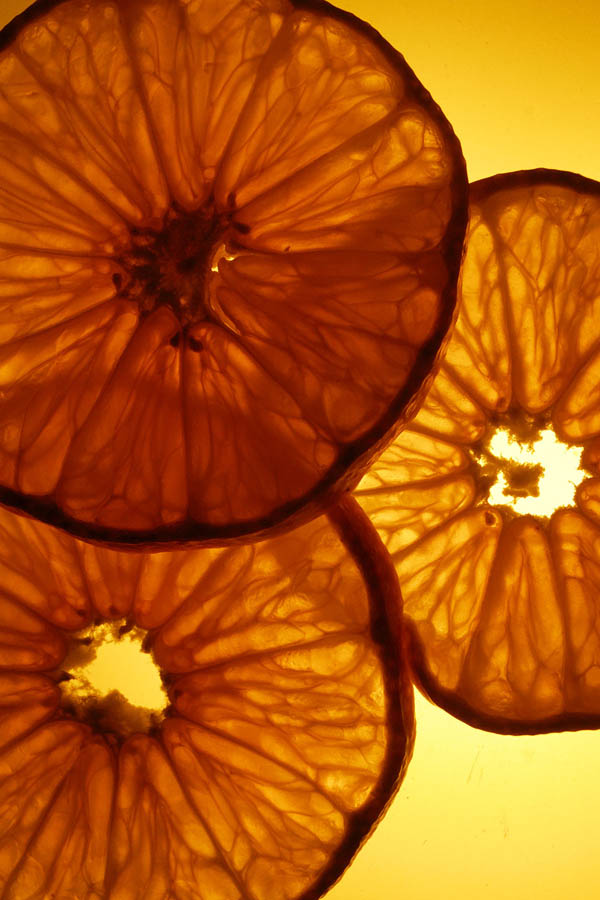
\includegraphics[width=0.6\linewidth,height=\textheight,keepaspectratio]{figuras0/citrus.jpg}

Essa experiência mostrou que o conhecimento científico não avança por
mera especulação, mas por \textbf{testes controlados e evidências
observáveis}, capazes de distinguir entre correlação e causalidade.

\section{A Ciência}\label{a-ciuxeancia}

\subsection{Perguntado ``Por que''}\label{perguntado-por-que}

O ponto de partida da ciência é a curiosidade sobre o mundo: \textbf{por
que as coisas acontecem da forma como acontecem?} Essa indagação,
aparentemente simples, é o motor que impulsiona toda investigação
científica. A ciência busca compreender não apenas o que ocorre, mas
também \textbf{as causas e mecanismos} subjacentes aos fenômenos
observados.

Durante séculos, especialmente até a metade do século XIX, o
conhecimento sobre diversos processos naturais era limitado. Na
medicina, por exemplo, pouco se sabia sobre doenças infecciosas e seus
modos de transmissão. Somente com os avanços de pesquisadores como
\textbf{Louis Pasteur} (1822--1895) é que se consolidou a \textbf{Teoria
Microbiana da Doença}, transformando profundamente a prática médica e a
saúde pública.

\subsection{Perguntado ``Por que''}\label{perguntado-por-que-1}

Antes desses avanços, outros cientistas já haviam dado contribuições
fundamentais à sistematização do conhecimento. Em 1662, \textbf{John
Graunt} publicou a primeira \textbf{tábua de mortalidade}, no livro
\emph{Natural and Political Observations Made upon the Bills of
Mortality}. Esse trabalho foi um dos primeiros esforços para quantificar
e descrever padrões populacionais e de saúde a partir de registros
empíricos.

Graunt aplicou raciocínios quantitativos a dados sobre nascimentos e
mortes, inaugurando a tradição estatística na análise de fenômenos
sociais e biológicos. Mais de dois séculos depois, Pasteur ampliou essa
lógica de observação e mensuração, demonstrando experimentalmente que
doenças contagiosas decorriam da ação de microrganismos, e desenvolvendo
o processo de \textbf{pasteurização} como medida de prevenção. Somente
em 1873 a academia de Medicina Francesa defende a tese que doenças
contagiosas e processos infecciosos tem os microrganismos como
responsáveis.

\begin{figure}[H]

{\centering \pandocbounded{
\includegraphics[keepaspectratio]{figuras0/t_mort.jpg}}

}

\caption{Uma das Primeiras Tábuas de Mortalidade}

\end{figure}%

Esses marcos ilustram como o avanço da ciência depende da capacidade de
observar, mensurar e explicar os fenômenos de maneira sistemática e
replicável.

\subsection{Objetivo da Ciência}\label{objetivo-da-ciuxeancia}

O propósito último da ciência é \textbf{tornar o mundo um lugar melhor
para vivermos}, por meio da geração de conhecimento e de inovação
tecnológica. Entretanto, o progresso técnico não ocorre isoladamente:
ele depende do \textbf{entendimento teórico} dos fenômenos.

A teoria é o que permite explicar o mundo de forma coerente, organizando
as observações em um quadro interpretativo. É a partir dela que se
formulam hipóteses, se testam explicações e se criam soluções práticas.
Assim, \textbf{as inovações técnicas são frutos do entendimento
teórico}, e não o contrário, sendo que a boa ciência combina observação
empírica com reflexão conceitual.

\subsection{O Uso Inadequado da
Ciência}\label{o-uso-inadequado-da-ciuxeancia}

Embora a ciência tenha transformado profundamente o modo como
compreendemos o mundo, seu prestígio também pode ser utilizado de forma
indevida. A invocação do termo ``científico'' muitas vezes é empregada
para \textbf{atribuir credibilidade a afirmações infundadas}, criando
uma aparência de legitimidade sem o devido rigor metodológico.

\begin{tcolorbox}[enhanced jigsaw, leftrule=.75mm, coltitle=black, colframe=quarto-callout-warning-color-frame, toprule=.15mm, opacitybacktitle=0.6, bottomtitle=1mm, bottomrule=.15mm, titlerule=0mm, toptitle=1mm, title=\textcolor{quarto-callout-warning-color}{\faExclamationTriangle}\hspace{0.5em}{Credibilidade Fake}, arc=.35mm, breakable, opacityback=0, colbacktitle=quarto-callout-warning-color!10!white, colback=white, left=2mm, rightrule=.15mm]

Nada confere mais autoridade a uma alegação do que a sugestão de que ela
foi ``comprovada cientificamente'' ou ``baseada em evidências
científicas''.

\end{tcolorbox}

\pandocbounded{
\includegraphics[keepaspectratio]{figuras0/fakenews.jpg}}

No entanto, nem toda afirmação que se apresenta como científica é, de
fato, resultado de um processo de investigação rigoroso. É comum
encontrar exemplos de \textbf{pseudociência}, discursos que simulam o
formato da ciência, mas carecem de fundamentos empíricos verificáveis.

Afirmações de que \textbf{extraterrestres visitaram a Terra}, de que
\textbf{plantas sentem prazer e dor}, ou de que \textbf{celulares causam
tumores cerebrais}, são exemplos de como o rótulo ``científico'' pode
ser usado de maneira enganosa.

Da mesma forma, \textbf{teorias conspiratórias}, como a ideia de que
governos ocultam informações sobre eventos históricos, frequentemente se
valem de uma retórica pseudoacadêmica para convencer o público. Esses
casos ilustram como a aparência de método pode ser usada para mascarar a
ausência de evidência.

\section{Método Científico}\label{muxe9todo-cientuxedfico}

\textbf{Observar, Explicar e Testar}

O método científico se organiza em três etapas principais: observar,
propor explicações e testar. Cada uma delas é essencial para transformar
dados em conhecimento confiável e orientar a investigação de forma
estruturada.

\subsection{Observar}\label{observar}

Observar significa ter uma \textbf{noção clara dos fatos} que envolvem o
fenômeno que estamos estudando. \textbf{Ciência é a arte de fazer boas
observações}, capazes de identificar e focar nos aspectos mais
relevantes do que está acontecendo. \textbf{A observação fornece pistas}
sobre por que um fenômeno ocorre e permite avaliar se diferentes
explicações podem ser plausíveis ou devem ser descartadas.

\pandocbounded{
\includegraphics[keepaspectratio]{figuras0/observation.png}}

\begin{tcolorbox}[enhanced jigsaw, leftrule=.75mm, coltitle=black, colframe=quarto-callout-note-color-frame, toprule=.15mm, opacitybacktitle=0.6, bottomtitle=1mm, bottomrule=.15mm, titlerule=0mm, toptitle=1mm, title=\textcolor{quarto-callout-note-color}{\faInfo}\hspace{0.5em}{Nem sempre a observação é simples ou direta.}, arc=.35mm, breakable, opacityback=0, colbacktitle=quarto-callout-note-color!10!white, colback=white, left=2mm, rightrule=.15mm]

O processo de observar pode ser limitado por dados insuficientes ou
difíceis de acessar. É importante reconhecer essas dificuldades e
trabalhar para minimizar seus efeitos.

\end{tcolorbox}

\subsubsection{Observções devem ser:}\label{observuxe7uxf5es-devem-ser}

\begin{itemize}
\tightlist
\item
  Ter clara noção de quais os fenômenos relevantes
\item
  Encontramos uma maneira de garantir que não negligenciamos nada no
  processo de fazer nossas observações?
\item
  Não viesada: Cegueira a mudança e Cegueira desatenta
  \url{https://www.youtube.com/watch?v=FaAIW8WFBq8}
\item
  O que sabemos com certeza? O que é baseado em fatos e o que é baseado
  em conjecturas ou suposição?

  \begin{itemize}
  \tightlist
  \item
    Evite suposições inocentemente incorporadas
  \end{itemize}
\item
  Consideramos alguma informação comparativa necessária?
\item
  As nossas observações foram contaminadas por expectativas ou crenças?
\end{itemize}

\subsubsection{Como conseguir boas observações e evitar
viéses?}\label{como-conseguir-boas-observauxe7uxf5es-e-evitar-viuxe9ses}

Para alcançar observações mais precisas, é importante recorrer a
\textbf{instrumentos} que ampliem nossos sentidos e utilizar
\textbf{medições quantitativas} que descrevam os fenômenos de forma mais
fiel. Assim, reduzimos as distorções que decorrem da percepção humana e
obtemos registros mais objetivos e verificáveis.

\begin{center}
\pandocbounded{
\includegraphics[keepaspectratio]{figuras0/computador.png}}
\end{center}

\begin{center}
\pandocbounded{\includegraphics[keepaspectratio]{figuras0/instrumento1.png}}
\end{center}

\subsection{Propor Explicação}\label{propor-explicauxe7uxe3o}

Explicar é apresentar um conjunto de fatores que \textbf{mostram como}
ou \textbf{por que um efeito ocorreu}. É o momento de propor uma
história explicativa, uma conjectura que, se verdadeira, daria sentido
ao fenômeno observado.

Perguntas como \textbf{``por que o sol nasce e se põe todos os dias?''}
ilustram esse tipo de esforço. Vejamos:

O Primeiro a enteder o nascimento do sol foi \textbf{Nicolau Copérnico
(1473-1543)}, que propôs o modelo heliocêntrico do sistema solar.
Segundo esse modelo, a Terra gira em torno do Sol, o que explica o
movimento aparente do sol no céu ao longo do dia.

Entretanto, as primeiras provas vieram quase século depois com
\textbf{Galileu , 1610}, com as observações de Venus e as fases da Lua.
Interessantemente, em 1633 Galileu Galilei foi julgado e condenado pela
Inquisição Católica pela sua defesa do heliocentrismo.

\begin{figure}[H]

{\centering 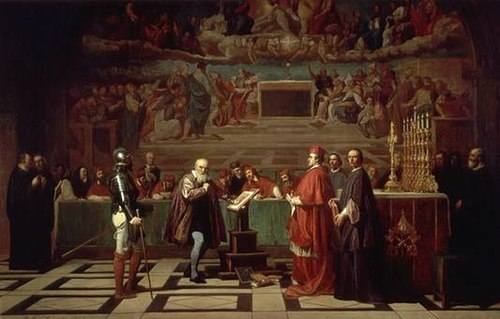
\includegraphics[width=0.5\linewidth,height=\textheight,keepaspectratio]{figuras0/galileu.jpg}

}

\caption{Galileo e o Santo Ofício, século XIX por Joseph-Nicolas
Robert-Fleury}

\end{figure}%

\begin{figure}[H]

{\centering \pandocbounded{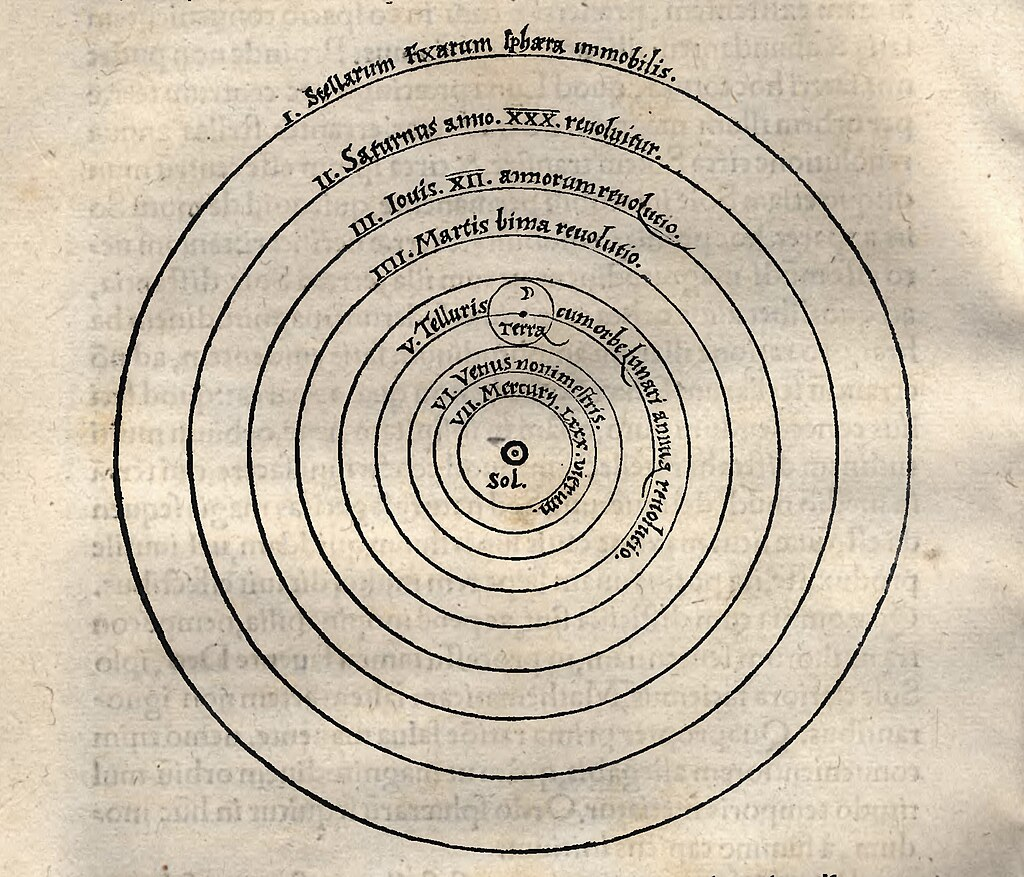
\includegraphics[keepaspectratio]{figuras0/copernico.jpg}}

}

\caption{De revolutionibus orbium coelestium}

\end{figure}%

\begin{tcolorbox}[enhanced jigsaw, leftrule=.75mm, coltitle=black, colframe=quarto-callout-note-color-frame, toprule=.15mm, opacitybacktitle=0.6, bottomtitle=1mm, bottomrule=.15mm, titlerule=0mm, toptitle=1mm, title=\textcolor{quarto-callout-note-color}{\faInfo}\hspace{0.5em}{História Explicativa}, arc=.35mm, breakable, opacityback=0, colbacktitle=quarto-callout-note-color!10!white, colback=white, left=2mm, rightrule=.15mm]

Portanto, a primeira etapa na tentativa de dar \textbf{sentido a um
conjunto de fatos} intrigantes é propor o que poderíamos chamar de uma
história explicativa, um conjunto de conjecturas que, se verdadeiras,
explicariam o quebra-cabeça.

\end{tcolorbox}

\subsubsection{Uma Boa Explicação}\label{uma-boa-explicauxe7uxe3o}

Uma \textbf{hipótese} é uma explicação provisória e ainda não comprovada
sobre algo específico Oferece uma explicação para um gama mais limitada
de fenômenos , um único evento ou um fato.

Já uma \textbf{teoria} é um corpo de conhecimento mais amplo e
consolidado, construído a partir de múltiplas verificações e evidências,
como as teorias do Big Bang, Teoria da evolução ou dos germes das
doenças.

\subsubsection{CUIDADO}\label{cuidado}

\begin{tcolorbox}[enhanced jigsaw, leftrule=.75mm, coltitle=black, colframe=quarto-callout-warning-color-frame, toprule=.15mm, opacitybacktitle=0.6, bottomtitle=1mm, bottomrule=.15mm, titlerule=0mm, toptitle=1mm, title=\textcolor{quarto-callout-warning-color}{\faExclamationTriangle}\hspace{0.5em}{Importante}, arc=.35mm, breakable, opacityback=0, colbacktitle=quarto-callout-warning-color!10!white, colback=white, left=2mm, rightrule=.15mm]

É comum ouvirmos \textbf{``isso é apenas uma teoria''}, como se fosse
uma opinião. No entanto, na ciência, uma teoria é uma explicação
robusta, apoiada por evidências e testes repetidos.

\end{tcolorbox}

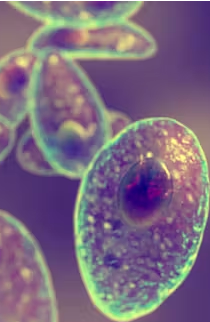
\includegraphics[width=0.4\linewidth,height=\textheight,keepaspectratio]{figuras0/teoria.png}

\subsubsection{Vamos Pensar: Obsedidade no
Brasil}\label{vamos-pensar-obsedidade-no-brasil}

Os brasileiros enfrentam um sério problema de peso. Entre 2006 e 2019, o
número de pessoas com sobrepeso ou obesidade aumentou em 72\%, chegando
a 20\% da população. Esses dados nos convidam a construir hipóteses que
expliquem o fenômeno, mesmo que provisoriamente. O objetivo não é
acertar, mas exercitar o raciocínio explicativo.

\begin{tcolorbox}[enhanced jigsaw, leftrule=.75mm, coltitle=black, colframe=quarto-callout-warning-color-frame, toprule=.15mm, opacitybacktitle=0.6, bottomtitle=1mm, bottomrule=.15mm, titlerule=0mm, toptitle=1mm, title=\textcolor{quarto-callout-warning-color}{\faExclamationTriangle}\hspace{0.5em}{Fatos e Observações}, arc=.35mm, breakable, opacityback=0, colbacktitle=quarto-callout-warning-color!10!white, colback=white, left=2mm, rightrule=.15mm]

Segundo a pesquisa Vigitel do Ministério da Saúde, para população acima
de 18 anos o percentual de pessoas com obesidade subiu de 11,8\% em 2006
para 20,3\% em 2019.

\end{tcolorbox}

\textbf{Quais as suas hipóteses para explicar esse fenômeno?} Não
precisa estar correta, mas deve explicar o fenômeno, caso seja
verdadeira.

\subsection{Testar Explicação}\label{testar-explicauxe7uxe3o}

Testar uma explicação significa verificar se suas previsões se
confirmam.

\textbf{Primeiro}, observam-se as consequências da explicação, o que
deveria acontecer se a explicação estiver correta?

\textbf{Segundo}, desenha-se um experimento ou estudo para confrontar
essa previsão com os dados. Se os resultados estiverem de acordo,
seguimos na direção certa; se não, a hipótese precisa ser revisada.

\pandocbounded{
\includegraphics[keepaspectratio]{figuras0/test.png}}

\begin{tcolorbox}[enhanced jigsaw, leftrule=.75mm, coltitle=black, colframe=quarto-callout-important-color-frame, toprule=.15mm, opacitybacktitle=0.6, bottomtitle=1mm, bottomrule=.15mm, titlerule=0mm, toptitle=1mm, title=\textcolor{quarto-callout-important-color}{\faExclamation}\hspace{0.5em}{Fácil Falar Difícil Fazer}, arc=.35mm, breakable, opacityback=0, colbacktitle=quarto-callout-important-color!10!white, colback=white, left=2mm, rightrule=.15mm]

Apesar da simplicidade do método científico em teoria, sua aplicação
prática exige cuidado e rigor.

\end{tcolorbox}

\section{A Causalidade}\label{a-causalidade}

Compreender a causalidade é uma das tarefas centrais da ciência. Depois
de observar um fenômeno e propor uma explicação, é preciso determinar se
existe de fato uma \textbf{relação causal} entre os fatores envolvidos.
Nem toda associação observada implica causalidade: dois eventos podem
ocorrer juntos sem que um cause o outro.

\section{Tipos de Estudos e Relações Causais: Randomização, estudos
prospectivos e
retrospectivos}\label{tipos-de-estudos-e-relauxe7uxf5es-causais-randomizauxe7uxe3o-estudos-prospectivos-e-retrospectivos}

\subsection{Estudos Causais
Randomizados.}\label{estudos-causais-randomizados.}

Os estudos causais baseados em randomização partem de um conjunto de
sujeitos que, antes do início do estudo, apresentam características
\textbf{muito semelhantes}. Nenhum desses sujeitos foi previamente
exposto ao agente causal suspeito. A partir daí, eles são
\textbf{aleatoriamente} designados para dois grupos: um \textbf{grupo de
tratamento} e um \textbf{grupo de controle}. Somente os sujeitos do
grupo de tratamento são expostos à causa sob investigação.

Esse tipo de desenho permite isolar o efeito da variável causal e
reduzir a influência de outros fatores.

No entanto, trata-se da forma mais \textbf{rara} de estudo nas
\textbf{Ciências Sociais Aplicadas}, em razão das dificuldades éticas e
práticas de implementação.

\subsubsection{Exemplos de Randomized Control Trial (RCT) em Ciências
Sociais e
Direito}\label{exemplos-de-randomized-control-trial-rct-em-ciuxeancias-sociais-e-direito}

\textbf{Justiça Restaurativa em Casos de Crimes Violentos}

\begin{itemize}
\item
  \textbf{Estudo}: Sherman, Lawrence W., et al.~\emph{Effects of
  face-to-face restorative justice on victims of crime in four
  randomized, controlled trials.} \textbf{Journal of experimental
  criminology} 1.3 (2005): 367-395.
\item
  \textbf{Objetivo}: O estudo avaliou o impacto de programas de justiça
  restaurativa, onde as vítimas e ofensores se encontram em conferências
  mediadas, em casos de crimes violentos - quatro experimentos
  controlados.
\item
  \textbf{Resultado}: As meta-análises das oito estimativas sugerem o
  sucesso da justiça restaurativa, tanto como um ritual de interação
  quanto como uma política para reduzir os danos às vítimas.
\end{itemize}

\begin{center}
\pandocbounded{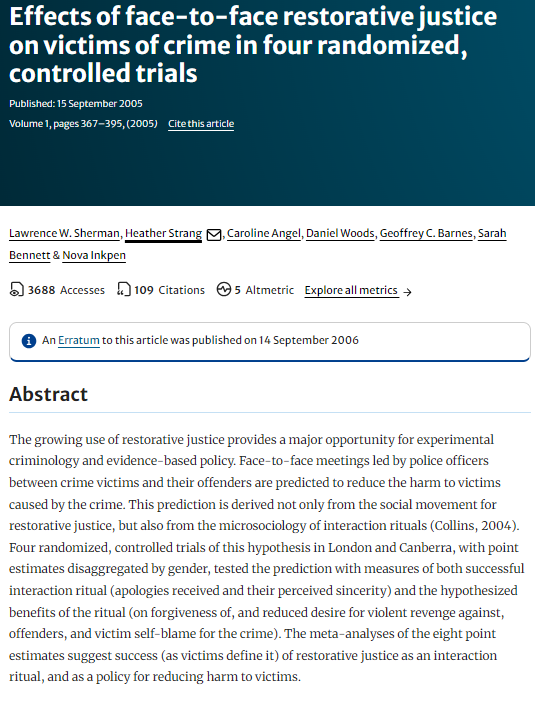
\includegraphics[keepaspectratio]{figuras0/restaurativa.png}}
\end{center}

\subsection{Estudos Prospectivos.}\label{estudos-prospectivos.}

Os estudos prospectivos, por sua vez, iniciam com sujeitos que
\textbf{já foram expostos ao agente causal} sob investigação e os
\textbf{acompanham ao longo do tempo}. O ponto de partida é uma situação
em que o resultado ainda é desconhecido, e o objetivo é identificar como
determinadas variáveis influenciam o desfecho futuro.

Esse tipo de estudo é valioso para observar a evolução dos efeitos
causais, mas é importante reconhecer que \textbf{outros fatores} podem
ser responsáveis por alguma parte do \textbf{efeito nos grupos tratado e
de controle}. Assim, a relação identificada pode ser relacional, mas não
necessariamente causal.

\subsubsection{Exemplos de Estudos Prospectivos em Ciências Sociais e
Direito}\label{exemplos-de-estudos-prospectivos-em-ciuxeancias-sociais-e-direito}

Um exemplo clássico de estudo prospectivo é o \emph{Million Women Study}
(2003), que investigou a relação entre terapias de reposição hormonal
(TRH) e câncer de mama.

\begin{itemize}
\tightlist
\item
  \textbf{Estudo}: Beral, Valerie, et al.~\emph{``Breast cancer and
  hormone-replacement therapy: the Million Women Study.''} \textbf{The
  Lancet} 362.9392 (2003): 1330-1331
\item
  \textbf{Objetivo}: O Million Women Study foi criado para investigar os
  efeitos de tipos específicos de TRH no câncer de mama incidente e
  fatal.Foram recrutadas 1.084.110 mulheres do Reino Unido com idades
  entre 50 e 64 anos para o Million Women Study entre 1996 e 2001.
\item
  \textbf{Resultado}: O uso atual de TRH está \textbf{associado} a um
  risco aumentado de câncer de mama incidente e fatal.
\end{itemize}

\begin{center}
\pandocbounded{
\includegraphics[keepaspectratio]{figuras0/prospectivo.png}}
\end{center}

\subsection{Estudos Causais
Retrospectivos.}\label{estudos-causais-retrospectivos.}

Nos estudos retrospectivos, o processo é inverso: \textbf{parte-se do
resultado final} e busca-se identificar as \textbf{causas que o
originaram}. Esses estudos têm como propósito principal identificar
fatores que levaram a determinado desfecho.

Geralmente, o pesquisador trabalha com dois grupos, controle e
tratamento, compostos por indivíduos que apresentam, ou não, o efeito
analisado. O desafio é identificar, de forma cuidadosa, os diferentes
níveis do fator potencial de causa entre esses grupos.

\begin{tcolorbox}[enhanced jigsaw, leftrule=.75mm, coltitle=black, colframe=quarto-callout-tip-color-frame, toprule=.15mm, opacitybacktitle=0.6, bottomtitle=1mm, bottomrule=.15mm, titlerule=0mm, toptitle=1mm, title=\textcolor{quarto-callout-tip-color}{\faLightbulb}\hspace{0.5em}{Explicando com Exemplo}, arc=.35mm, breakable, opacityback=0, colbacktitle=quarto-callout-tip-color!10!white, colback=white, left=2mm, rightrule=.15mm]

Efeitos do chumbo em crianças. Pesquisa com 4.000 crianças de 4 e 15
anos entre 1999 e 2002. Incluiu 135 crianças com transtorno de déficit
de atenção e hiperatividade (TDAH). Exames de sangue foram feitos em
todas as 4.000.

\begin{itemize}
\tightlist
\item
  As 135 crianças com TDAH apresentaram níveis de chumbo no sangue muito
  maior do que nas outras crianças.

  \begin{itemize}
  \tightlist
  \item
    Tinham quatro vezes mais probabilidade de ter níveis elevados de
    chumbo no sangue
  \end{itemize}
\end{itemize}

A \textbf{Questão} é, pode-se concluir que a exposição ao chumbo pode
causar TDAH?

\end{tcolorbox}

Mesmo os melhores estudos retrospectivos oferecem apenas evidências
limitadas de causalidade, pois é extremamente difícil controlar todos os
fatores potenciais que podem interferir na relação observada. Por isso,
é fundamental interpretar seus resultados com cautela.

Observa-se que Correspondência reversa às vezes é possível em estudos
retrospectivos. Ou seja TDAH -\textgreater{} Chumbo\ldots.

\begin{itemize}
\tightlist
\item
  E é esse o caso nesse estudo: crianças com TDAH são mais propensas a
  comer tinta com chumbo ou inalar pó de tinta por causa de sua
  hiperatividade.
\end{itemize}

\begin{tcolorbox}[enhanced jigsaw, leftrule=.75mm, coltitle=black, colframe=quarto-callout-warning-color-frame, toprule=.15mm, opacitybacktitle=0.6, bottomtitle=1mm, bottomrule=.15mm, titlerule=0mm, toptitle=1mm, title=\textcolor{quarto-callout-warning-color}{\faExclamationTriangle}\hspace{0.5em}{Cuidado}, arc=.35mm, breakable, opacityback=0, colbacktitle=quarto-callout-warning-color!10!white, colback=white, left=2mm, rightrule=.15mm]

Apesar de crianças com TDAH terem ``quatro vezes mais chance'' de ter
níveis elevados de chumbo no sangue.

\textbf{NÃO PODEMOS CONCLUIR QUE}: Crianças com níveis elevados de
chumbo têm ``quatro vezes mais probabilidade'' de ter TDAH.

\end{tcolorbox}

\subsubsection{Exemplos de Estudos Retrospectivos em Ciências Sociais e
Direito}\label{exemplos-de-estudos-retrospectivos-em-ciuxeancias-sociais-e-direito}

Um exemplo aplicado às Ciências Sociais é o estudo de Severi, FC; Jesus
Filho, J. 2022 (\emph{``Há diferenças remuneratórias por gênero na
magistratura brasileira?.''}), que investigou a hipótese de diferenças
remuneratórias entre juízes e juízas em oito tribunais de justiça
brasileiros.

\begin{itemize}
\item
  \textbf{Estudo} Severi, FC; Jesus Filho, J. \emph{``Há diferenças
  remuneratórias por gênero na magistratura brasileira?.''}
  \textbf{Revista de Administração Pública} 56.2 (2022): 208-225.
\item
  \textbf{Objetivo}: testar a hipótese de que há clara diferença entre
  as remunerações médias percebidas por juízes e juízas de 8 tribunais
  de justiça brasileiros.
\item
  \textbf{Resultado}: As diferenças nas médias remuneratórias persistem
  mesmo após o pareamento, o que pode ser explicado pelos mediadores de
  gênero, que operam gerando melhores oportunidades para homens em
  desfavor das mulheres.
\end{itemize}

\begin{center}
\pandocbounded{
\includegraphics[keepaspectratio]{figuras0/remuneracao.png}}
\end{center}

\subsection{O Método Científico segundo Richard
Feynman}\label{o-muxe9todo-cientuxedfico-segundo-richard-feynman}

Richard Feynman enfatiza que o método científico baseia-se em propor
hipóteses, derivar previsões e testá-las por meio da observação e do
experimento. Se os resultados não confirmam a previsão, a hipótese deve
ser rejeitada, independentemente de sua origem. Assim segundo o autor
temos o seguinte percurso:

\begin{itemize}
\tightlist
\item
  \textbf{Faça uma Observação}

  \begin{itemize}
  \tightlist
  \item
    Observe um fenômeno no mundo natural.
  \end{itemize}
\item
  \textbf{Formule uma Hipótese}

  \begin{itemize}
  \tightlist
  \item
    Crie uma possível explicação para o fenômeno.
  \end{itemize}
\item
  \textbf{Faça Previsões}

  \begin{itemize}
  \tightlist
  \item
    Preveja o que acontecerá se sua hipótese estiver correta.
  \end{itemize}
\item
  \textbf{Teste com Experimentos}

  \begin{itemize}
  \tightlist
  \item
    Conduza experimentos para testar as previsões.
  \end{itemize}
\item
  \textbf{Reavalie a Hipótese}

  \begin{itemize}
  \tightlist
  \item
    Se os resultados não batem com as previsões, a hipótese está errada.
  \end{itemize}
\end{itemize}

Essa visão mostra que a ciência é, acima de tudo, um compromisso ético
com a verdade empírica e a disposição de submeter ideias à crítica. O
método científico é mais do que um procedimento: é uma atitude de
curiosidade, dúvida e verificação constante.

\section{Buscando um Bom Instrumento:
Jurimetria}\label{buscando-um-bom-instrumento-jurimetria}

\subsection{O que é Jurimetria?}\label{o-que-uxe9-jurimetria}

A jurimetria nasce da aplicação do método científico ao campo do
Direito. Utiliza \textbf{ferramentas quantitativas e estatísticas para
analisar fenômenos jurídicos}, buscando identificar padrões, prever
comportamentos e fundamentar decisões em evidências empíricas. Mais do
que contar processos ou descrever dados, a jurimetria procura
\textbf{compreender os mecanismos} que orientam as decisões judiciais e
\textbf{revelar as regularidades} que estruturam a prática
jurídica.Assim como nas demais ciências, seu processo envolve observar,
explicar e testar

Um dos grandes \textbf{desafios} dessa abordagem está na própria
\textbf{natureza dos dados jurídicos}, que em sua maioria são não
estruturados. Decisões, petições e sentenças são \textbf{textos longos e
complexos}, redigidos em linguagem natural, o que torna sua análise
sistemática mais difícil.

Por isso, a pesquisa jurimétrica requer três etapas complementares:
\textbf{coletar e estruturar} os dados a partir de fontes dispersas;
aplicar \textbf{métodos de tratamento}, como limpeza, padronização e
categorização; e, por fim, empregar \textbf{métodos de análise
estatística} e computacional capazes de extrair padrões e formular
hipóteses sobre o funcionamento do sistema de justiça.

\begin{center}
\pandocbounded{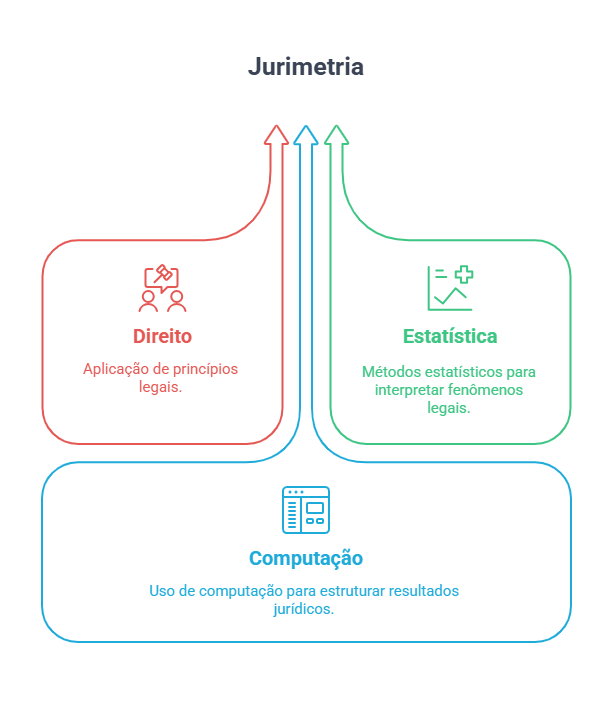
\includegraphics[keepaspectratio]{figuras0/jurimetria.png}}
\end{center}

Essa capacidade de transformar grandes volumes de informações textuais
não padronizadas em conhecimento empírico é o que confere à jurimetria
seu caráter verdadeiramente \textbf{interdisciplinar}, unindo
\textbf{Direito, Estatística e Ciência de Dados}.

\subsection{Porque estudar Jurimetria?}\label{porque-estudar-jurimetria}

O uso de informações e pesquisas empíricas no Direito permite
desenvolver práticas mais racionais, eficientes e transparentes. Entre
as principais finalidades dessa abordagem, destacam-se:

\begin{itemize}
\tightlist
\item
  \textbf{Aperfeiçoamento da gestão judiciária}, mediante o uso de dados
  para identificar gargalos, otimizar fluxos processuais e orientar
  decisões administrativas;
\item
  \textbf{Racionalização das decisões judiciais}, favorecendo maior
  consistência e previsibilidade nos julgamentos;
\item
  \textbf{Compreensão do funcionamento de leis e políticas públicas},
  avaliando seus efeitos práticos sobre o sistema de justiça e a
  sociedade;
\item
  \textbf{Avaliação criteriosa da implementação de normas e políticas},
  com base em indicadores objetivos e evidências empíricas.
\end{itemize}

Além de sua aplicação prática, a jurimetria também contribui para o
\textbf{desenvolvimento do senso crítico} diante de argumentos causais
frequentemente utilizados no cotidiano jurídico. A análise empírica
possibilita questionar afirmações do tipo:\\
- ``A jurisprudência dominante informa que\ldots{}'',\\
- ``O comportamento da vítima foi determinante para o desfecho do
caso'',\\
- ``Não há discriminação contra mulheres na carreira da magistratura
paulista'',\\
- ``Juízes seguem o entendimento do Ministério Público''.

Esses exemplos evidenciam a necessidade de examinar, com base em dados e
métodos, até que ponto tais alegações se sustentam empiricamente.

\begin{figure}[H]

{\centering \pandocbounded{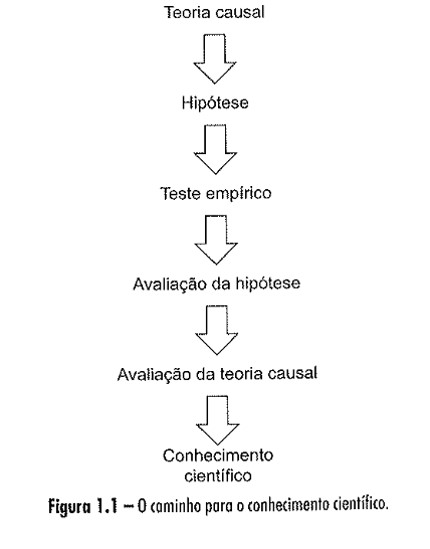
\includegraphics[keepaspectratio]{figuras0/metodo_jur.jpg}}

}

\caption{Paul Kellstedt,Guy Whitten . Fundamentos da pesquisa em ciência
política}

\end{figure}%

\subsection{O que Jurimetria pode
Responder?}\label{o-que-jurimetria-pode-responder}

A jurimetria pode oferecer evidências que \textbf{apoiem a tomada de
decisão} e \textbf{o aperfeiçoamento institucional}, seja no Judiciário,
no Legislativo ou no Executivo. Alguns exemplos ilustram o tipo de
questão que a jurimetria pode responder:

\begin{figure}[H]

{\centering \pandocbounded{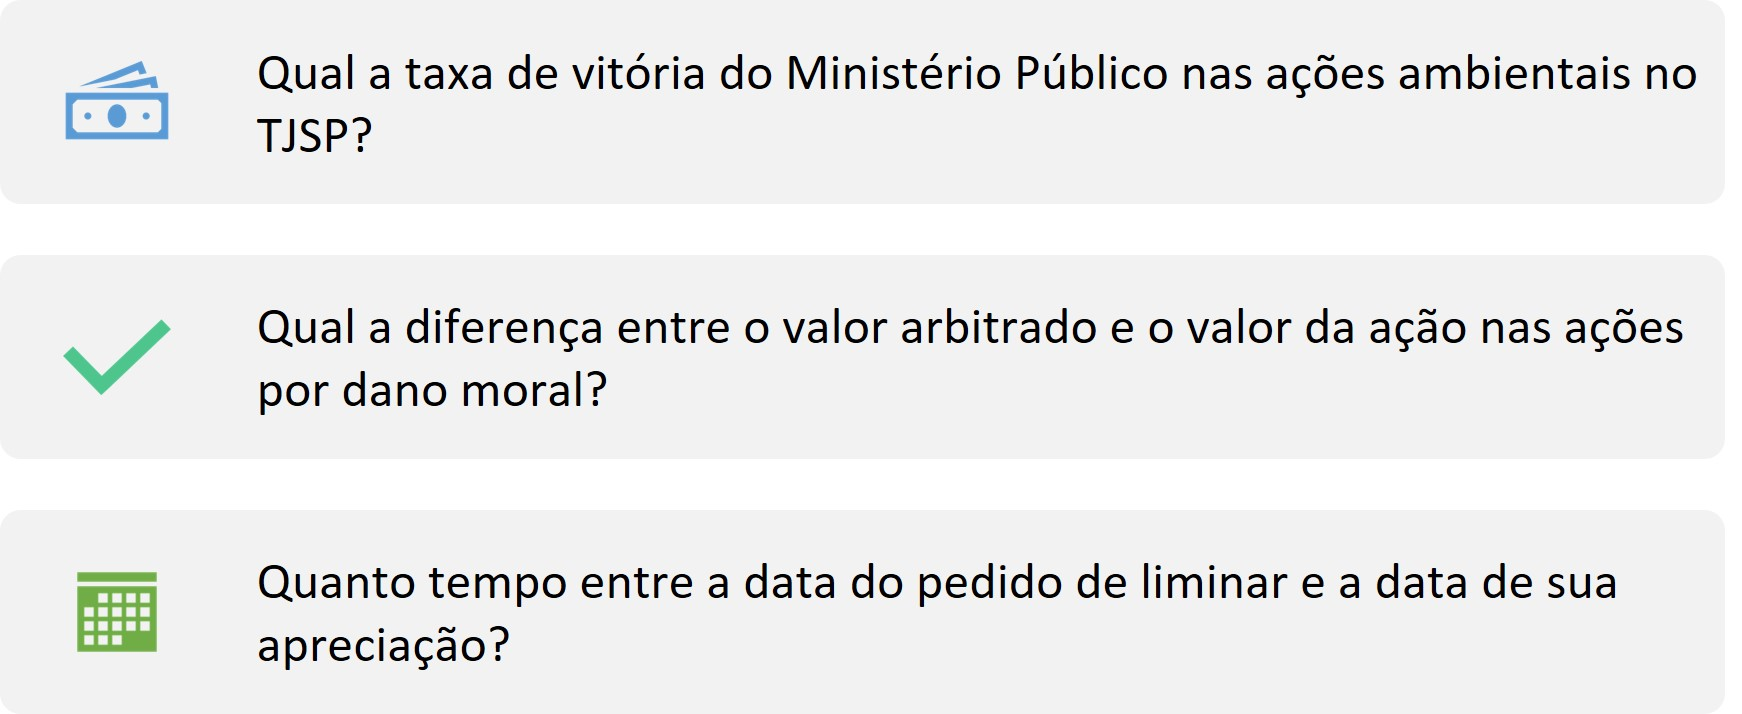
\includegraphics[keepaspectratio]{figuras0/resposta1.jpg}}

}

\caption{Severi, F.}

\end{figure}%

A jurimetria busca quantificar e \textbf{compreender padrões e
comportamentos} do sistema de justiça Com isso, oferece uma base
empírica para aprimorar o Direito e orientar políticas públicas e
reformas mais objetiva e transparente.

\subsection{O que IA Pode Fazer?}\label{o-que-ia-pode-fazer}

Na jurimetria, a função da \textbf{inteligência artificial} (IA) é
automatizar a extração de informações de peças processuais, analisar
rapidamente grandes volumes de texto e, até auxiliar na elaboração de
documentos jurídicos. A perspectiva é que a IA \textbf{apoie a atividade
do Direito}, oferecendo suporte e eficiência, mas \textbf{não substitua
o papel do profissional jurídico}. Assim:

\begin{figure}[H]

{\centering \pandocbounded{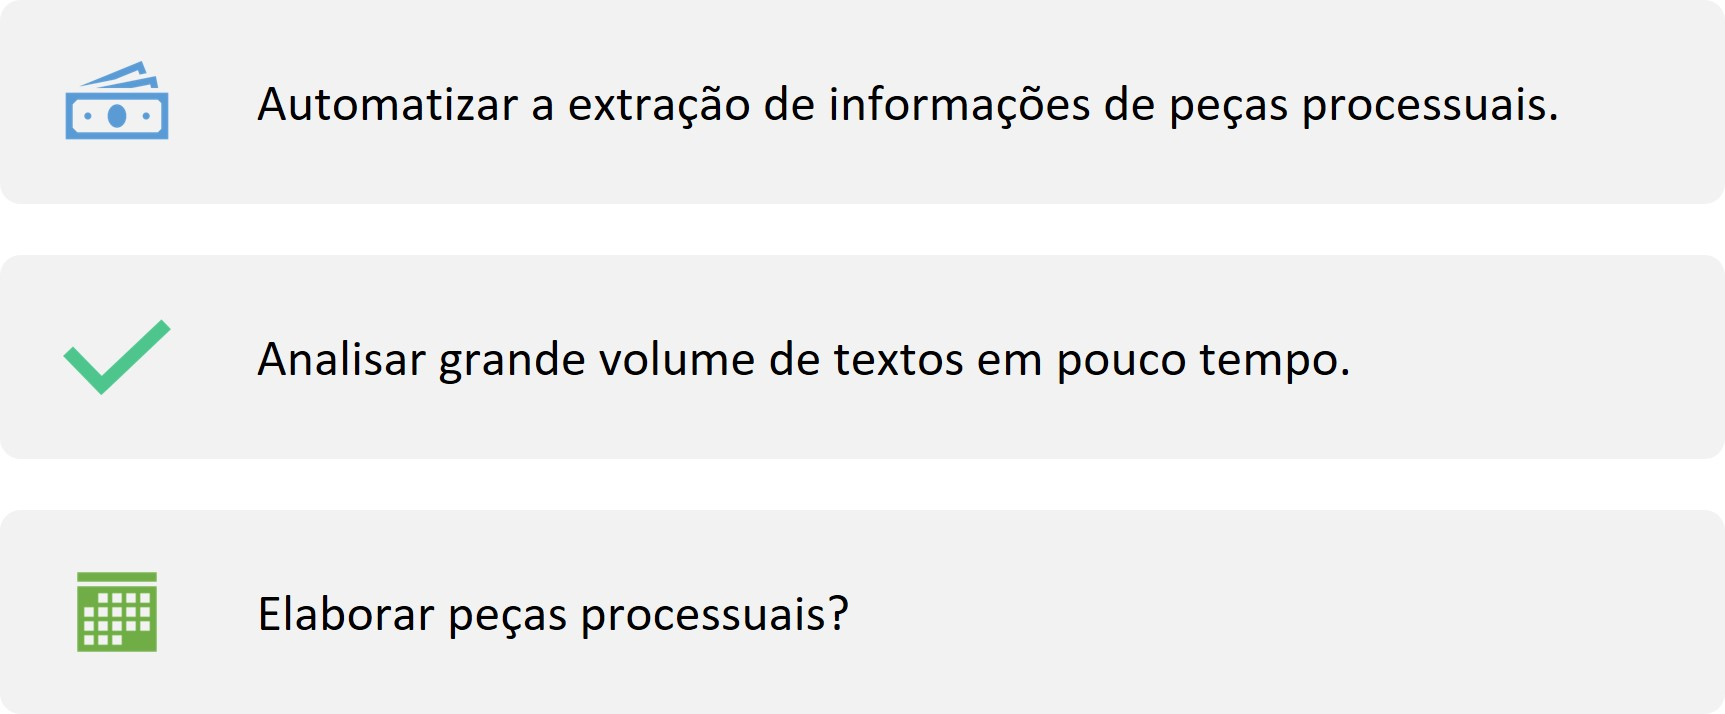
\includegraphics[keepaspectratio]{figuras0/ia.jpg}}

}

\caption{Severi, F.}

\end{figure}%

\section{Fase 1: Boas Obervações: Coleta e
Transformação}\label{fase-1-boas-obervauxe7uxf5es-coleta-e-transformauxe7uxe3o}

\subsection{Coleta e Transformação de
Dados}\label{coleta-e-transformauxe7uxe3o-de-dados}

A fase de \textbf{coleta e transformação} de dados é uma \textbf{etapa
central} na pesquisa jurimétrica, funcionando como o \textbf{alicerce}
do trabalho, já que todas as análises posteriores dependem da qualidade
e da estruturação desses dados.

Geralmente, a coleta é realizada por meio de consultas aos sites dos
tribunais, mas esses acervos não oferecem a totalidade das sentenças e
acórdãos, e possivelmente não constituem uma amostra totalmente
representativa. Por isso, é fundamental conduzir essa etapa com cautela,
rigor e transparência, reconhecendo suas limitações e discutindo como
essas incompletudes podem impactar os resultados das pesquisas.

\begin{figure}[H]

{\centering \pandocbounded{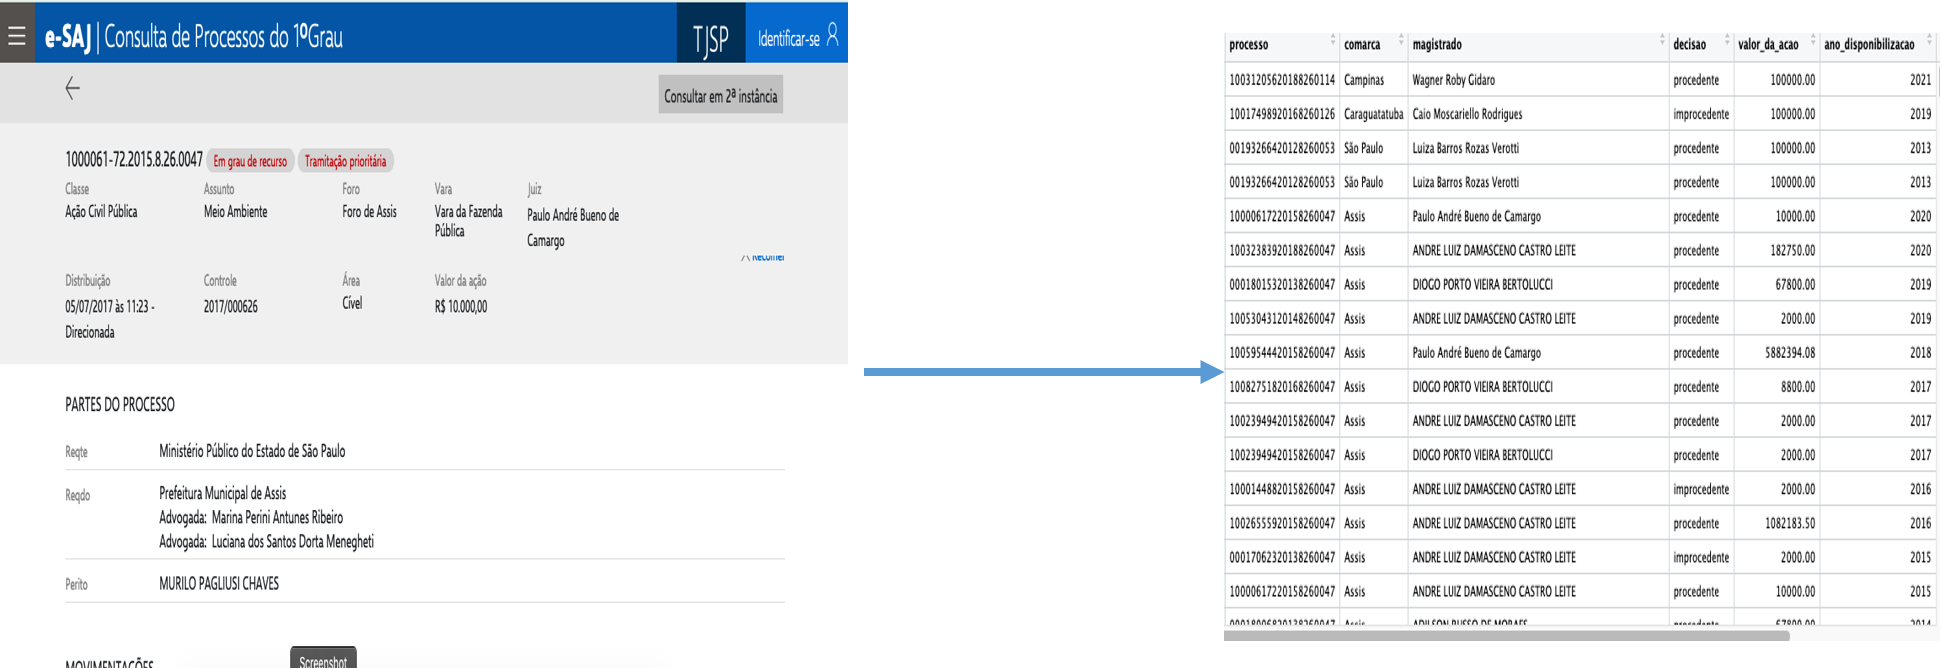
\includegraphics[keepaspectratio]{figuras0/coleta.png}}

}

\caption{Severi, F.}

\end{figure}%

\subsection{Extração com IA}\label{extrauxe7uxe3o-com-ia}

Outra etapa essencial na construção do banco de dados é o uso de
\textbf{inteligência artificial}. Embora a IA seja poderosa, ela não é
totalmente precisa, dependendo da forma como os \textbf{textos
processuais estão escritos e dos léxicos utilizados}. Pode deixar de
identificar termos relevantes ou interpretá-los fora de contexto. Por
isso, essa etapa deve ser conduzida com cuidado, incluindo testes em
subamostras, para garantir que os prompts retornem as informações
desejadas

\begin{figure}[H]

{\centering \pandocbounded{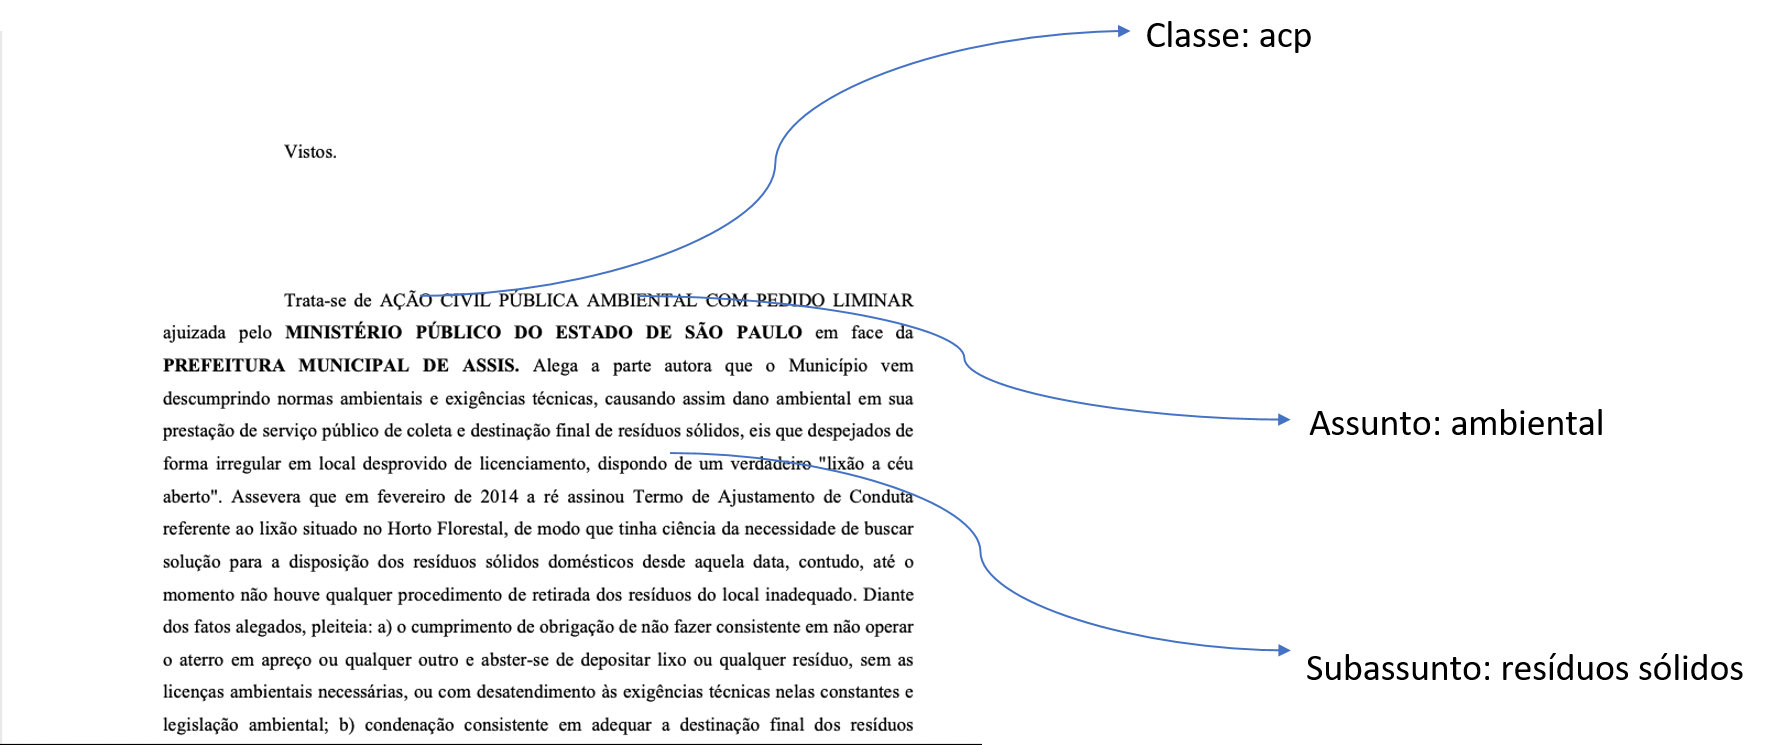
\includegraphics[keepaspectratio]{figuras0/ia2.png}}

}

\caption{Severi, F.}

\end{figure}%

\begin{figure}[H]

{\centering \pandocbounded{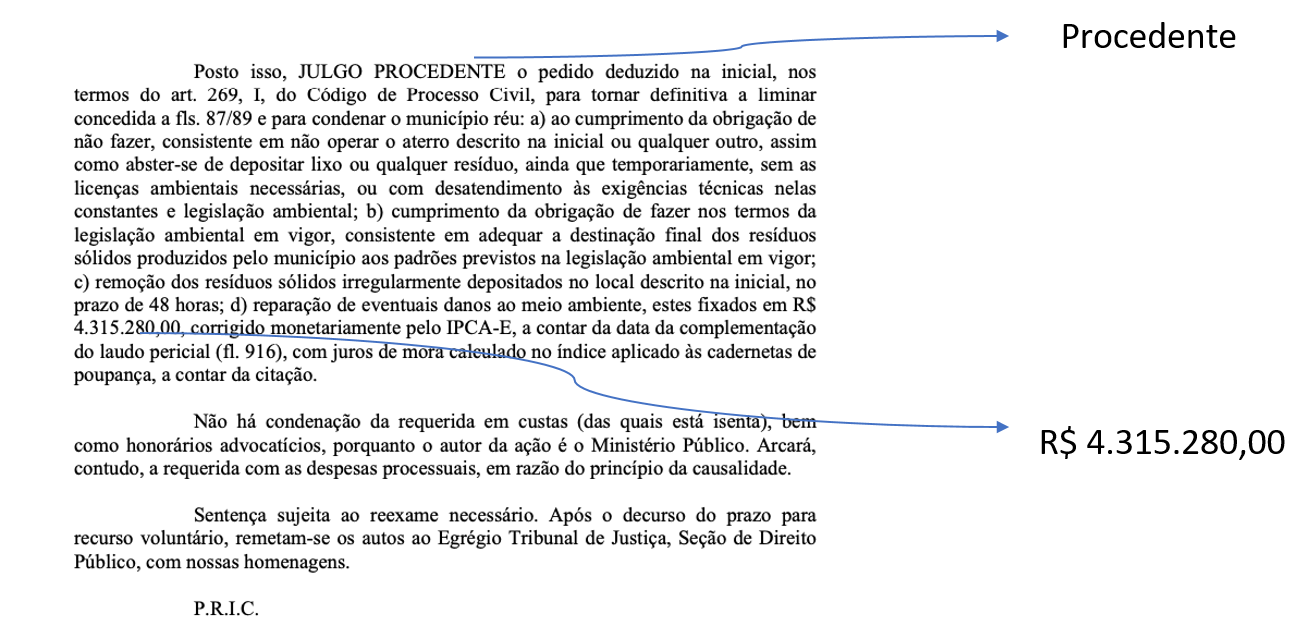
\includegraphics[keepaspectratio]{figuras0/ia3.png}}

}

\caption{Severi, F.}

\end{figure}%

\subsection{Bom conhecimento de
programação}\label{bom-conhecimento-de-programauxe7uxe3o}

O conhecimento de linguagens de programação voltadas à ciência de dados,
como \texttt{R} e \texttt{Python}, é fundamental para coletar, tratar e
analisar dados jurídicos. Além disso, é desejável dominar sistemas de
gerenciamento de bancos de dados, \texttt{SQL} p.ex., pois permite
armazenar esses dados de forma eficiente. Por fim, é importante utilizar
técnicas de extração e análise de texto, como \texttt{NLP} e
\textbf{expressões regulares}, para explorar e organizar as informações
de maneira adequada.

\section{Fase 2: Explicações}\label{fase-2-explicauxe7uxf5es}

\subsection{Teoria do Direito}\label{teoria-do-direito}

O \textbf{conhecimento} substantivo do \textbf{Direito} é fundamental
para elaborar perguntas apropriadas, levantar hipóteses e delimitar o
escopo de um projeto. Há muitos ramos no direito e dentro desses ramos
muitos assuntos:

\begin{itemize}
\tightlist
\item
  Direito civil
\item
  Direito penal
\item
  Direito tributário
\item
  Direito previdenciário
\item
  Direito do Trabalho
\item
  Direito administrativo
\item
  Direito constitucional
\end{itemize}

Ter pessoas que entendam bem sobre o tema é fundamental para o sucesso
do projeto.

\subsection{Bom conhecimento do
Direito}\label{bom-conhecimento-do-direito}

Conforme observa Ricardo Feliz, cada esfera do Poder possui seus
próprios atos processuais. Os \textbf{atos processuais} são o registro
formal das \textbf{ações dentro de um processo}. Compreender esses atos
é fundamental para determinar quando e como coletar as informações
dentro da estrutura processual. Algus exemplos de atos processuais no
Judiciários são:

\begin{itemize}
\tightlist
\item
  Sentença; Acórdão; Decisão liminar; Decisão monocrática
\item
  Petição inicial; Contestação
\item
  Parecer
\item
  Documentos probatórios
\end{itemize}

Ter clareza sobre esses atos permite organizar a coleta de dados de
forma precisa e consistente, garantindo que cada informação seja
extraída no momento adequado do processo.

\begin{figure}[H]

{\centering \pandocbounded{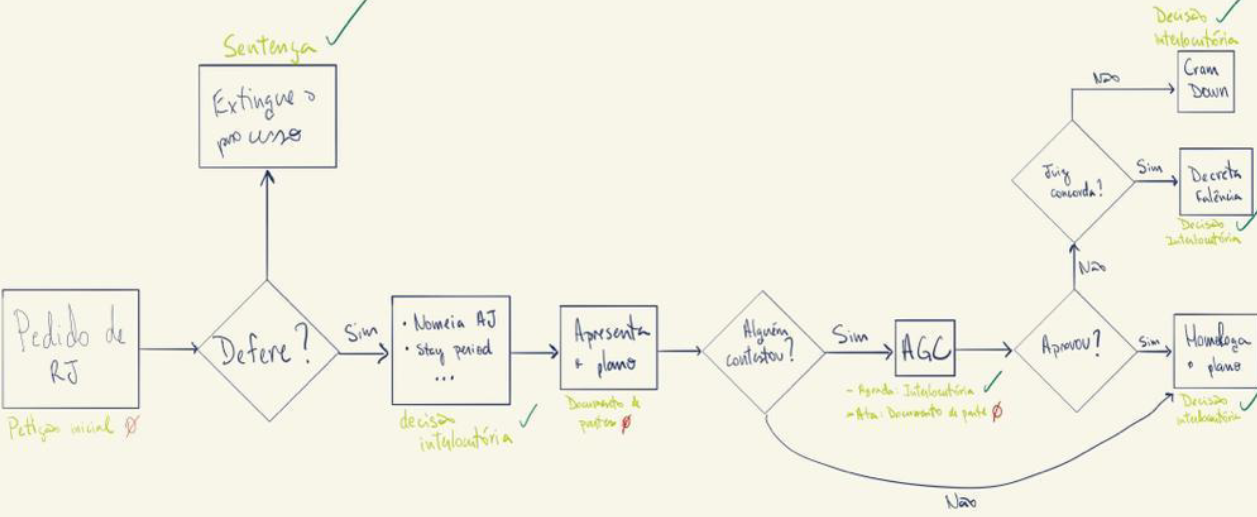
\includegraphics[keepaspectratio]{figuras0/ricardo.png}}

}

\caption{Feliz, R.}

\end{figure}%

\subsection{Bom Desenho de Projeto}\label{bom-desenho-de-projeto}

Para elaborar um bom projeto, é essencial seguir uma lógica que conecte
problema, hipótese e dados:

\begin{itemize}
\tightlist
\item
  \textbf{Compreender o fenômeno:} identificar claramente o problema
  existente e entender bem o contexto em que ele ocorre.\\
\item
  \textbf{Definir o objetivo da pesquisa:} estabelecer o que se pretende
  responder sobre o fenômeno.\\
\item
  \textbf{Planejar como responder:} determinar quais informações
  precisam ser coletadas e como serão analisadas para testar a hipótese.
\end{itemize}

Um bom projeto articula essas etapas de forma coerente, garantindo que
cada decisão metodológica esteja alinhada com o problema inicial e a
pergunta de pesquisa.

\begin{tcolorbox}[enhanced jigsaw, leftrule=.75mm, coltitle=black, colframe=quarto-callout-warning-color-frame, toprule=.15mm, opacitybacktitle=0.6, bottomtitle=1mm, bottomrule=.15mm, titlerule=0mm, toptitle=1mm, title=\textcolor{quarto-callout-warning-color}{\faExclamationTriangle}\hspace{0.5em}{Exemplo}, arc=.35mm, breakable, opacityback=0, colbacktitle=quarto-callout-warning-color!10!white, colback=white, left=2mm, rightrule=.15mm]

\begin{itemize}
\tightlist
\item
  Qual o tempo estimado para a apreciação de uma liminar em pedido de
  despejo?
\item
  A quantidade e o tipo de droga influenciam o desfecho processual no
  sentido de condenar por tráfico ou por porte?
\item
  Decisões monocráticas são mais relevantes que decisões colegiadas no
  STF?
\end{itemize}

\end{tcolorbox}

\subsection{Importante!!!}\label{importante-1}

A \textbf{avaliação de viabilidade} é uma etapa essencial no desenho de
um projeto de pesquisa. Ela busca responder três perguntas básicas:

\begin{itemize}
\tightlist
\item
  Os dados existem?\\
\item
  Se existem, são acessíveis?\\
\item
  Se são acessíveis, qual a qualidade desses dados?
\end{itemize}

\section{Fase 3: Análise das
Explicações}\label{fase-3-anuxe1lise-das-explicauxe7uxf5es}

\subsection{Usando Modelos e
Estatística}\label{usando-modelos-e-estatuxedstica}

\textbf{Análises descritivas}: resume e organiza os dados para mostrar
padrões e distribuições. Abaixo pode-se observar o comportamento de
9.499 julgados com o assunto direito ambiental no TJSP.

Após organizar os dados em tabelas, manteve-se apenas ações civis
públicas. Técnicas de processamento de linguagem natural classificaram
os desfechos (como procedente, improcedente, acordo, extinção, etc.) e
os casos foram agrupados por autor (MP, Defensoria, Executivo e Terceiro
Setor) e por faixa de valor da causa. Essa análise permite observar a
distribuição dos julgados por desfecho, autor e valor, fornecendo uma
visão inicial do comportamento judicial.

\begin{figure}[H]

{\centering \pandocbounded{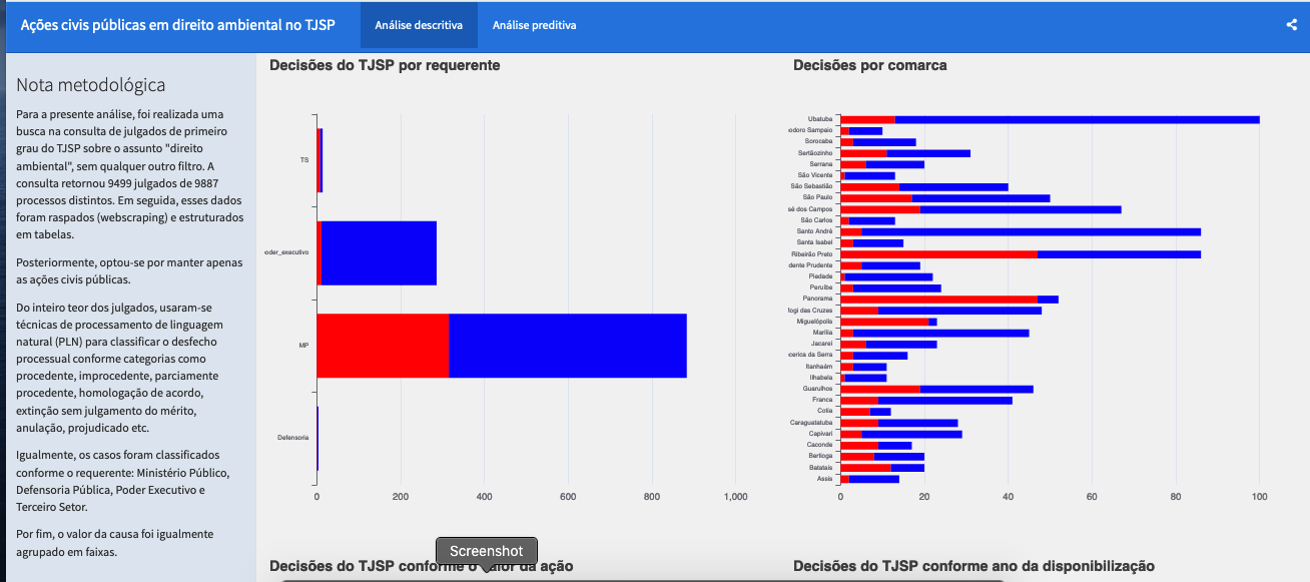
\includegraphics[keepaspectratio]{figuras0/descritiva.png}}

}

\caption{Severi, F.}

\end{figure}%

\begin{center}\rule{0.5\linewidth}{0.5pt}\end{center}

\textbf{Análises Preditivas}: usa dados e modelos para antecipar
resultados futuros.

Na análise preditiva, é possível estimar a probabilidade de uma ação
civil pública em Direito Ambiental no TJSP, por exemplo, na comarca de
Assis, ser julgada procedente, considerando que o requerente é o
Ministério Público.

\begin{figure}[H]

{\centering \pandocbounded{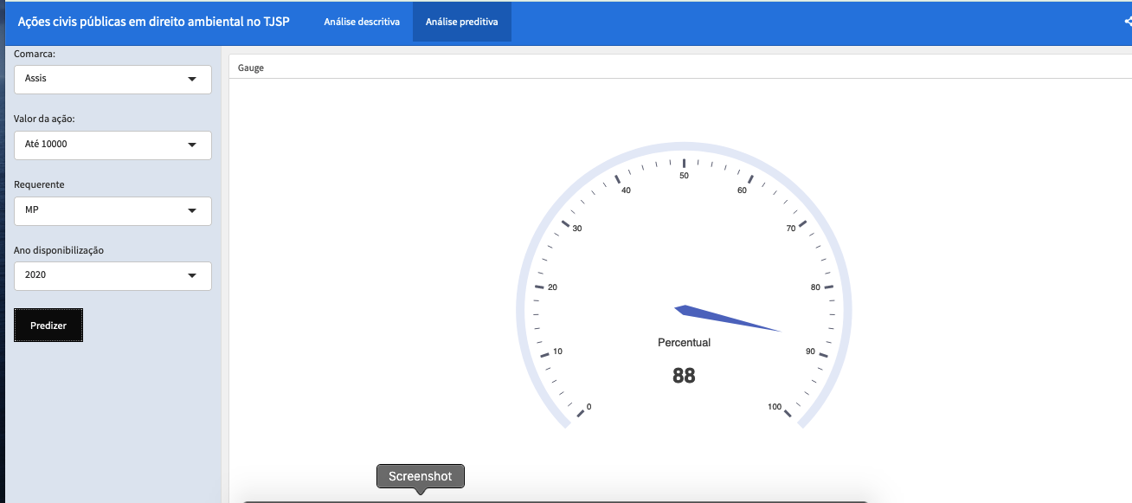
\includegraphics[keepaspectratio]{figuras0/preditiva.png}}

}

\caption{Severi, F.}

\end{figure}%

\begin{center}\rule{0.5\linewidth}{0.5pt}\end{center}

\textbf{Análises Explicartivas}: investiga relações e/ou causas entre
variáveis para entender por que os fenômenos ocorrem.

Neste modelo, busca-se \textbf{explicar o diferencial de salário} entre
magistrados homens e mulheres, \textbf{identificando os determinantes}
que efetivamente causam essa diferença. Ou seja, o objetivo é entender
por que o diferencial observado ocorre.

\begin{figure}[H]

{\centering \pandocbounded{
\includegraphics[keepaspectratio]{figuras0/remuneracao.png}}

}

\caption{Severi, F.}

\end{figure}%

\subsection{Ciclo da Pesquisa}\label{ciclo-da-pesquisa}

O ciclo da pesquisa nem sempre segue um caminho linear ou fácil;
frequentemente é tortuoso. Apesar disso, ele envolve etapas importantes
que precisam ser bem fundamentadas e respeitadas, como as que segue:

\begin{itemize}
\tightlist
\item
  Desenho do projeto;
\item
  Operacionalização em variáveis mensuráveis;
\item
  Análise de viabilidade;
\item
  Coleta;
\item
  Limpeza e organização dos dados;
\item
  Transformação dos dados;
\item
  Análise exploratória;
\item
  Análise inferencial e preditiva;
\item
  Métricas de desempenho;
\item
  Publicação dos resultados.
\end{itemize}

\begin{figure}[H]

{\centering \pandocbounded{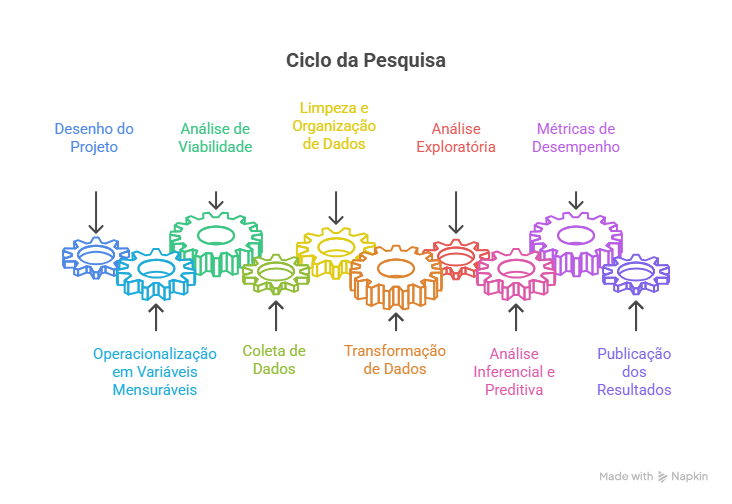
\includegraphics[keepaspectratio]{figuras0/ciclo_jur.png}}

}

\caption{Severi, F.}

\end{figure}%

\bookmarksetup{startatroot}

\chapter{Análise Descritiva}\label{anuxe1lise-descritiva}

Tirando Informação dos Dados

\hfill\break

\section{Cadeia de Valor do
Conhecimento}\label{cadeia-de-valor-do-conhecimento}

A construção do conhecimento é um caminho longo e complexo. A cadeia de
valor do conhecimento é um modelo que busca representar esse caminho.
Vejamos a Figura abaixo:

\begin{figure}[H]

{\centering 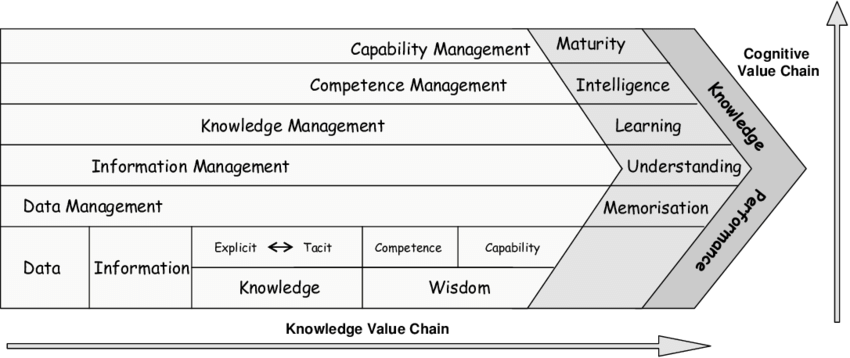
\includegraphics[width=0.8\linewidth,height=\textheight,keepaspectratio]{figuras/knowledgeVC.png}

}

\caption{Ermine, J.L (2013): Cadeia de Valor do Conhecimento}

\end{figure}%

Para cumprir esse longo percurso a Ciência de Dados tem um papel
fundamental na atualidade.

A Ciência de Dados é uma área interdisciplinar que combina conhecimentos
de estatística, matemática, computação, e no nosso caso do Direito, para
extrair conhecimento a partir de dados.

\begin{figure}[H]

{\centering 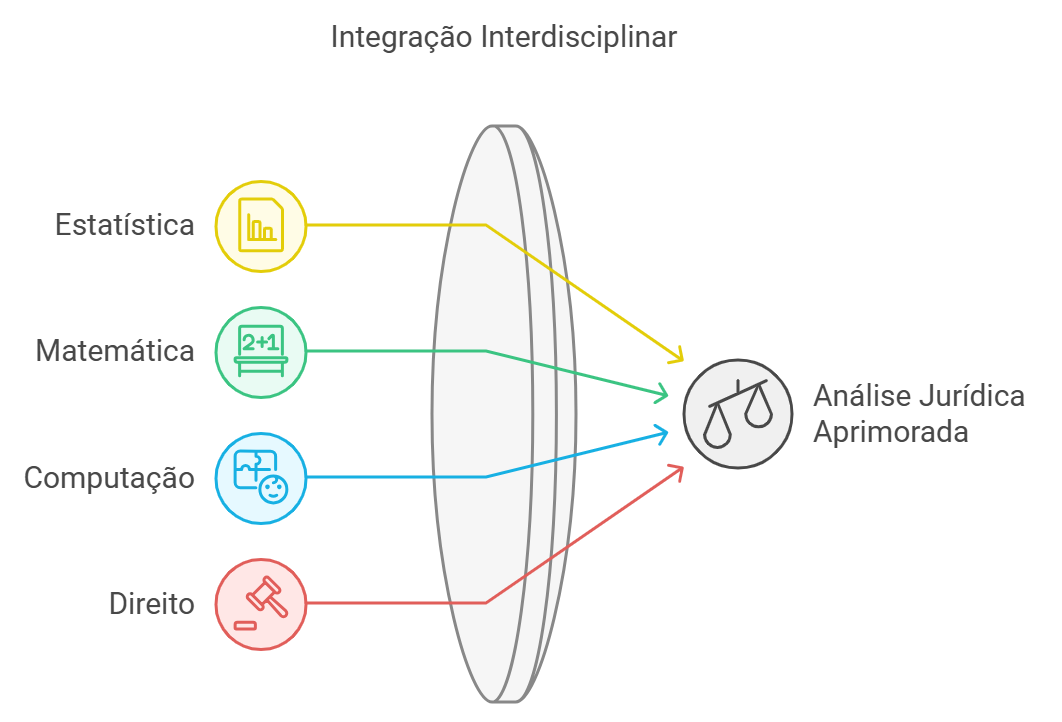
\includegraphics[width=0.7\linewidth,height=\textheight,keepaspectratio]{figuras/combina.png}

}

\caption{Estratégia Interdisciplinas}

\end{figure}%

A Ciência de Dados é um processo que envolve diversas etapas, como a
coleta de dados, a organização dos dados, a análise dos dados, a
interpretação dos resultados, entre outras. Vejamos a figura sobre ciclo
de vida da ciência de dados:

\begin{figure}[H]

{\centering 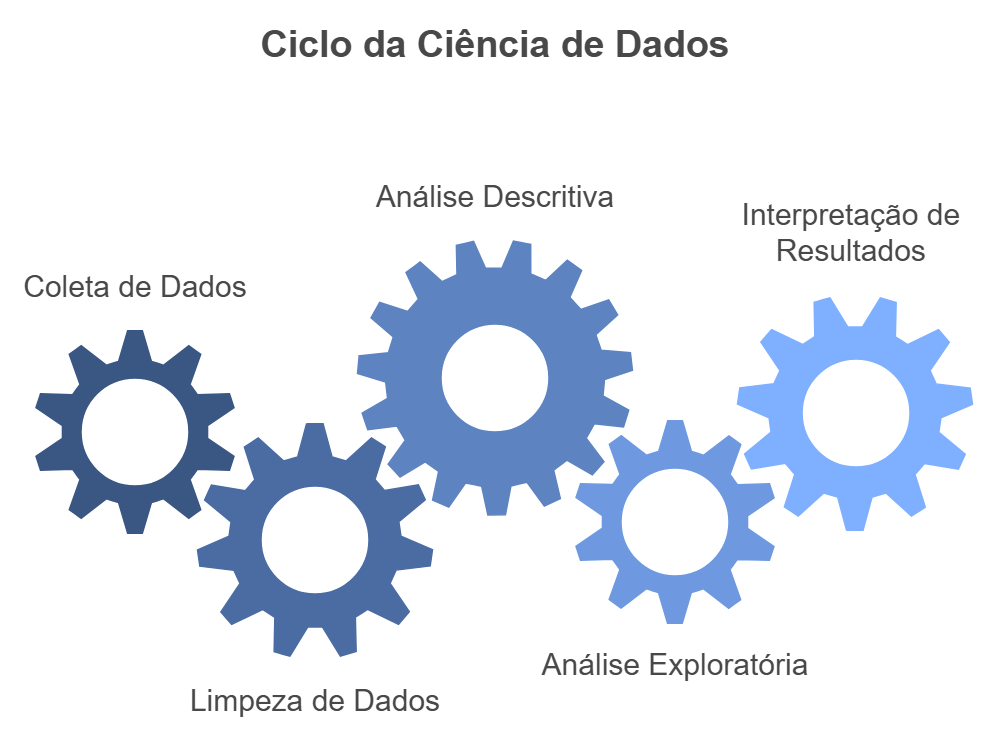
\includegraphics[width=0.7\linewidth,height=\textheight,keepaspectratio]{figuras/cicloDS.png}

}

\caption{Ciclo de Vida da Ciência de Dados}

\end{figure}%

O ciclo de vida da ciência de dados é um modelo que descreve as etapas
envolvidas no processo de análise de dados. Esse modelo é composto por
cinco etapas principais:

\begin{enumerate}
\def\labelenumi{\arabic{enumi}.}
\item
  \textbf{Coleta de Dados}: Busca de informações que possam ser úteis
  para responder a uma pergunta de pesquisa. Esses dados podem ser
  coletados de diversas fontes, como pesquisas de campo, bases de dados,
  entrevistas, entre outros.
\item
  \textbf{Limpar e Organização}: Pesquisador organiza os dados coletados
  de forma a facilitar a análise. Isso pode envolver a criação de
  tabelas, limpeza, estruturação, entre outros aspectos.
\item
  \textbf{Análise Descritiva}: Busca descrever os dados coletados de
  forma a identificar padrões, tendências, relações entre variáveis,
  entre outros aspectos. Isso pode envolver a utilização de estatísticas
  descritivas, gráficos, mapas, entre outros recursos.
\item
  \textbf{Análise Exploratória}: Explorar os dados coletados de forma a
  identificar padrões, tendências, relações entre variáveis, entre
  outros aspectos. Isso pode envolver a utilização de técnicas
  estatísticas mais avançadas, como regressão, análise de cluster,
  análise fatorial, entre outras.
\item
  \textbf{Interpretação dos Resultados}: Interpretar os resultados
  obtidos na análise descritiva e exploratória de forma a responder à
  pergunta de pesquisa. Isso pode envolver a elaboração de conclusões,
  recomendações, entre outros aspectos.
\end{enumerate}

\section{Estatísticas Descritivas: Medidas Numéricas a partir da
amostra}\label{estatuxedsticas-descritivas-medidas-numuxe9ricas-a-partir-da-amostra}

A análise descritiva é uma etapa fundamental no processo de análise de
dados. Ela consiste em descrever os dados coletados de forma a
identificar padrões, tendências, relações entre variáveis, entre outros
aspectos.

Vamos entender 3 padrões importantes nessa etapa:

\begin{enumerate}
\def\labelenumi{\arabic{enumi}.}
\item
  \textbf{Medidas de Posição}: São medidas que indicam a posição de um
  valor em relação aos demais valores de um conjunto de dados.
\item
  \textbf{Medidas de Variabilidade}: São medidas que indicam o grau de
  dispersão dos valores de um conjunto de dados.
\item
  \textbf{Medidas de Associação}: São medidas que indicam a relação
  entre duas ou mais variáveis de um conjunto de dados.
\end{enumerate}

Vamos entender os resultados dessas medidas para dois conjuntos
distintos de variáveis:

\begin{enumerate}
\def\labelenumi{\arabic{enumi}.}
\item
  \textbf{Variáveis Discretas}: São variáveis que podem assumir um
  número finito de valores. Por exemplo, o número de filhos de uma
  pessoa, o número de processos em uma Vara, procedente ou improcedente.
\item
  \textbf{Variáveis Contínuas}: São variáveis que podem assumir um
  número infinito de valores. Por exemplo, a renda per capita, a taxa de
  feminicídio, tempo do processo, dosimetria da pena.
\end{enumerate}

\textbf{CASO DE ESTUDO:}

Vamos tentar entender essas medidas a partir de um banco de dados real e
pequeno. Será utilizado um banco de dados extraído do
\href{https://publicacoes.forumseguranca.org.br/items/6b3e3a1b-3bd2-40f7-b280-7419c8eb3b39}{Anuário
da Segurança Pública (2023)}, com informações sobre a taxa de
feminicídio, a taxa de tentativa de feminicídio, a taxa de homicídio de
mulheres, a renda per capita, entre outras variáveis.

As medidas numéricas que veremos para as três padrões a serem observados
são:

\textbf{MEDIDAS DE POSIÇÃO:}

\begin{itemize}
\tightlist
\item
  Média,
\item
  Mediana,
\item
  Moda,
\item
  Percentis,
\item
  Quartis.
\end{itemize}

\textbf{MEDIDAS DE VARIABILIDADE:}

\begin{itemize}
\tightlist
\item
  Amplitude,
\item
  Amplitude interquartil,
\item
  Variância,
\item
  Desvio Padrão e
\item
  Coeficiente de Variação.
\end{itemize}

\textbf{MEDIDAS DE ASSOCIAÇÃO:}

\begin{itemize}
\tightlist
\item
  Covariancia e
\item
  Coeficiente de Correlção.
\end{itemize}

Vamos apresentar as fórmulas de algumas dessas principais
medidas.Primeiramente vams importantaro nosso banco de dados:

\begin{Shaded}
\begin{Highlighting}[]
\NormalTok{final\_fem\_22 }\OtherTok{\textless{}{-}} \FunctionTok{read.csv}\NormalTok{(}\StringTok{"C:/Users/Alexandre\_Nicolella/Aulas/FEA{-}RP/Jurimetria/jurimetria/final\_fem\_22.csv"}\NormalTok{, }\AttributeTok{head=}\NormalTok{T ,}\AttributeTok{sep=}\StringTok{";"}\NormalTok{)}
\end{Highlighting}
\end{Shaded}

ou

\begin{Shaded}
\begin{Highlighting}[]
\FunctionTok{install.packages}\NormalTok{(}\StringTok{"remotes"}\NormalTok{) }\CommentTok{\# baixar o pacote devtools}
\NormalTok{remotes}\SpecialCharTok{::}\FunctionTok{install\_github}\NormalTok{(}\StringTok{"jjesusfilho/cursoESMP"}\NormalTok{) }\CommentTok{\# baixar o pacote deste curso}
\FunctionTok{library}\NormalTok{(cursoESMP) }\CommentTok{\# carregar o pacote deste curso}
\NormalTok{final\_fem\_22}\OtherTok{\textless{}{-}}\NormalTok{cursoESMP}\SpecialCharTok{::}\NormalTok{final\_fem\_22}
\end{Highlighting}
\end{Shaded}

Visualizando as primeiras 10 linhas do banco de dados:

\begin{Shaded}
\begin{Highlighting}[]
\FunctionTok{library}\NormalTok{(kableExtra)}

\NormalTok{final\_fem\_22 }\SpecialCharTok{|\textgreater{}} 
  \FunctionTok{head}\NormalTok{(}\DecValTok{10}\NormalTok{) }\SpecialCharTok{|\textgreater{}} 
  \FunctionTok{kbl}\NormalTok{(}\AttributeTok{digits =} \DecValTok{2}\NormalTok{,  ) }\SpecialCharTok{\%\textgreater{}\%}
     \FunctionTok{kable\_styling}\NormalTok{()}
\end{Highlighting}
\end{Shaded}

\begin{table}
\centering
\begin{tabular}[t]{l|l|l|r|r|r|r|r|r|r|r|r|r|r|r}
\hline
sigla & estados & regiao & homic\_abs & homic\_tx & feminic\_abs & feminic\_tx & part\_feminic & rendapc & mais\_50 & t\_homic\_abs & t\_homic\_tx & t\_feminic\_abs & t\_feminic\_tx & part\_t\_feminic\\
\hline
AC & Acre & N & 22 & 5.3 & 11 & 2.6 & 50.0 & 1038 & 1 & 388 & 93.4 & 16 & 3.9 & 3.96\\
\hline
AL & Alagoas & NE & 73 & 4.5 & 31 & 1.9 & 42.5 & 935 & 0 & 160 & 9.8 & 54 & 3.3 & 25.23\\
\hline
AM & Amazonas & N & 88 & 4.5 & 21 & 1.1 & 23.9 & 965 & 0 & 83 & 4.2 & 45 & 2.3 & 35.16\\
\hline
AP & Amapa & N & 22 & 6.0 & 8 & 2.2 & 36.4 & 1177 & 0 & 95 & 25.9 & 44 & 12.0 & 31.65\\
\hline
BA & Bahia & NE & 406 & 5.6 & 107 & 1.5 & 26.4 & 1010 & 0 & 582 & 8.0 & 174 & 2.4 & 23.02\\
\hline
CE & Ceara & NE & 264 & 5.8 & 28 & 0.6 & 10.6 & 1050 & 0 & 324 & 7.2 & 102 & 2.3 & 23.94\\
\hline
DF & Distrito Federal & CO & 32 & 2.2 & 19 & 1.3 & 59.4 & 2913 & 1 & 208 & 14.2 & 88 & 6.0 & 29.73\\
\hline
ES & Espirito Santo & SD & 95 & 4.9 & 33 & 1.7 & 34.7 & 1723 & 0 & 450 & 23.1 & 70 & 3.6 & 13.46\\
\hline
GO & Goias & CO & 137 & 3.8 & 56 & 1.6 & 40.9 & 1619 & 0 & 364 & 10.2 & 168 & 4.7 & 31.58\\
\hline
MA & Maranhao & NE & 127 & 3.7 & 69 & 2.0 & 54.3 & 814 & 1 & 264 & 7.7 & 106 & 3.1 & 28.65\\
\hline
\end{tabular}
\end{table}

\begin{tcolorbox}[enhanced jigsaw, bottomrule=.15mm, leftrule=.75mm, arc=.35mm, colframe=quarto-callout-note-color-frame, breakable, opacityback=0, toprule=.15mm, colback=white, left=2mm, rightrule=.15mm]
\begin{minipage}[t]{5.5mm}
\textcolor{quarto-callout-note-color}{\faInfo}
\end{minipage}%
\begin{minipage}[t]{\textwidth - 5.5mm}

\vspace{-3mm}\textbf{Descrição do Banco de Dados}\vspace{3mm}

\begin{enumerate}
\def\labelenumi{\arabic{enumi}.}
\item
  \textbf{homic\_abs}: Número absoluto de homicídios feminínos
  registrados em 2022.
\item
  \textbf{homic\_tx}: Taxa de homicídios feminino 100 mil mulheres.
\item
  \textbf{feminic\_abs}: Número absoluto de feminicídios registrados em
  2022.
\item
  \textbf{feminic\_tx}: Taxa de feminicídios por 100 mil mulheres.
\item
  \textbf{part\_feminic}: Participação percentual dos feminicídios no
  total de homicídios femininos.
\item
  \textbf{rendapc}: Renda per capita do Estado.
\item
  \textbf{mais\_50}: Proporção de feminicídios acima de 50\%.
\item
  \textbf{t\_homic\_abs}: Número absoluto da tentativa de homicídios
  femininos
\item
  \textbf{t\_homic\_tx}: Taxa de tentativa de homicídios para 100 mil
  mulheres.
\item
  \textbf{t\_feminic\_abs}: Número absoluto de tentativa de
  feminicídios.
\item
  \textbf{t\_feminic\_tx}: Taxa de tentativa de feminicídios por 100 mil
  mulheres.
\item
  \textbf{part\_t\_feminic}: Participação percentual da tentativa de
  feminicídios em relação ao total de tentativas de homicídios
  femininos.
\end{enumerate}

\end{minipage}%
\end{tcolorbox}

\subsection{Gráficos no R}\label{gruxe1ficos-no-r}

O ggplot2 é um pacote do R utilizado para criar gráficos estatísticos de
forma poderosa e flexível. Apesar de parecer complexo, é fácil de
aprender, pois possui princípios básicos simples e poucos casos
excepcionais.O ggplot2 é projetado para ser utilizado iterativamente:
você começa com os dados brutos e adiciona camadas de anotações ou
resumos estatísticos.

\textbf{A GRAMÁTICA DOS GRÁFICOS}

O ggplot2 é um pacote do R que implementa a Grammar of Graphics
(Wilkinson, 2005), uma abordagem para criar gráficos estatísticos. Ele
organiza os gráficos em componentes fundamentais, permitindo
flexibilidade e personalização.

Um gráfico no ggplot2 é construído combinando os seguintes elementos:

\begin{enumerate}
\def\labelenumi{\arabic{enumi}.}
\tightlist
\item
  \textbf{Dados}: A base de dados a ser visualizada.
\item
  \textbf{Mapeamentos estéticos}(aes): Define como variáveis são
  associadas a atributos visuais (cor, forma, tamanho).
\item
  \textbf{Camadas} (layers): Compostas por:

  \begin{itemize}
  \tightlist
  \item
    \textbf{Geoms}: Elementos visuais - tipos de gráficos (pontos,
    linhas, barras).
  \item
    \textbf{Stats}: Transformações estatísticas ou ajustar modelos.
  \item
    \textbf{Escalas} (scales): Determina as esclaas de x e y (eixos,
    legendas, cores).
  \end{itemize}
\item
  \textbf{Sistemas de coordenadas} (coord): Define como os dados são
  posicionados no gráfico (ex.: cartesiano ou polar).
\item
  \textbf{Facetamento} (facet): Divide os dados em subconjuntos para
  gerar gráficos separados.
\item
  \textbf{Tema} (theme): Personaliza detalhes visuais, como fontes e
  cores de fundo.
\end{enumerate}

Clique abaixo para ver alguns tipos de gráficos que podem ser criados
com o ggplot2:

\begin{tcolorbox}[enhanced jigsaw, bottomrule=.15mm, leftrule=.75mm, arc=.35mm, colframe=quarto-callout-note-color-frame, breakable, opacityback=0, toprule=.15mm, colback=white, left=2mm, rightrule=.15mm]
\begin{minipage}[t]{5.5mm}
\textcolor{quarto-callout-note-color}{\faInfo}
\end{minipage}%
\begin{minipage}[t]{\textwidth - 5.5mm}

\vspace{-3mm}\textbf{Veja aqui Algumas Possibilidades de Camadas}\vspace{3mm}

\begin{itemize}
\tightlist
\item
  \texttt{geom\_area()}: cria um gráfico de área.\\
\item
  \texttt{geom\_density()}: cria um gráfico de densidade de kernel.\\
\item
  \texttt{geom\_dotplot()}: cria um gráfico de pontos.\\
\item
  \texttt{geom\_freqpoly()}: cria um polígono de frequência.\\
\item
  \texttt{geom\_histogram()}: cria um histograma.\\
\item
  \texttt{stat\_ecdf()}: plota a função de densidade acumulada
  empírica.\\
\item
  \texttt{stat\_qq()}: cria um gráfico quantil-quantil.\\
\item
  \texttt{geom\_bar()}: cria um gráfico de barras.
\end{itemize}

\end{minipage}%
\end{tcolorbox}

Vejamos um exemplo inicial de um gráfico da taxa de homicídio feminino e
a taxa de feminicídio por Estado no Brasil

Primeiro, definindo os dados que serão utilizados e os eixos x e y,
vejamos o que ocorre:

\begin{Shaded}
\begin{Highlighting}[]
\FunctionTok{library}\NormalTok{(ggplot2)}
\FunctionTok{ggplot}\NormalTok{(}\AttributeTok{data =}\NormalTok{ final\_fem\_22, }\FunctionTok{aes}\NormalTok{(}\AttributeTok{x =}\NormalTok{ homic\_tx, }\AttributeTok{y =}\NormalTok{ feminic\_tx))}
\end{Highlighting}
\end{Shaded}

\pandocbounded{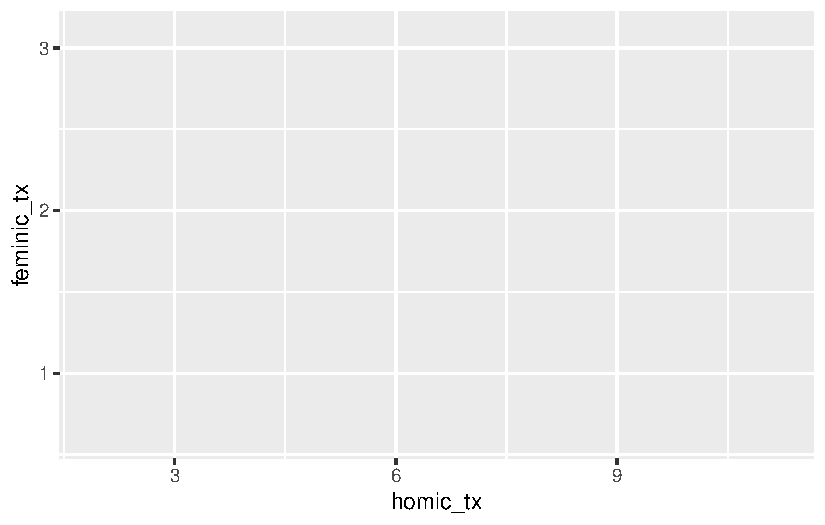
\includegraphics[keepaspectratio]{descritiva_v2_files/figure-pdf/unnamed-chunk-4-1.pdf}}

Agora podemos adicionar uma camada de pontos ao gráfico:

\begin{Shaded}
\begin{Highlighting}[]
\FunctionTok{ggplot}\NormalTok{(}\AttributeTok{data =}\NormalTok{ final\_fem\_22, }\FunctionTok{aes}\NormalTok{(}\AttributeTok{x =}\NormalTok{ homic\_tx, }\AttributeTok{y =}\NormalTok{ feminic\_tx))}\SpecialCharTok{+}
  \FunctionTok{geom\_point}\NormalTok{()}
\end{Highlighting}
\end{Shaded}

\pandocbounded{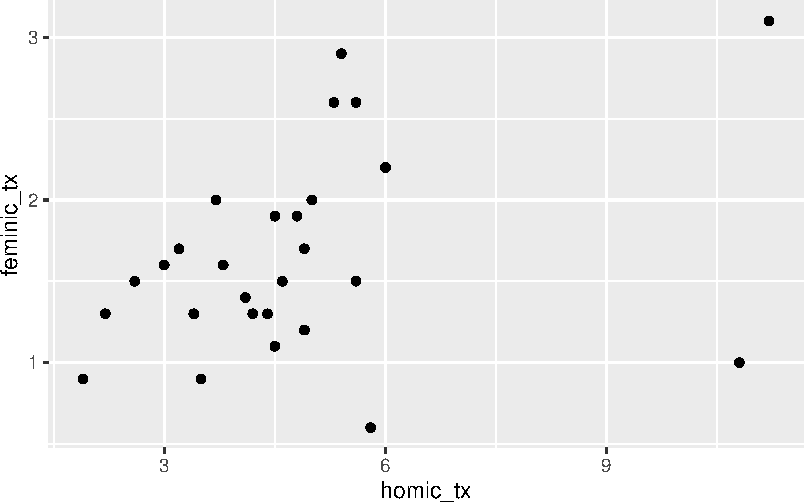
\includegraphics[keepaspectratio]{descritiva_v2_files/figure-pdf/unnamed-chunk-5-1.pdf}}

Podemos fazer com que cada ponto seja associado a uma região do Brasil:

\begin{Shaded}
\begin{Highlighting}[]
\FunctionTok{ggplot}\NormalTok{(}\AttributeTok{data =}\NormalTok{ final\_fem\_22, }\FunctionTok{aes}\NormalTok{(}\AttributeTok{x =}\NormalTok{ homic\_tx, }\AttributeTok{y =}\NormalTok{ feminic\_tx, }\AttributeTok{colour=}\NormalTok{regiao))}\SpecialCharTok{+}
  \FunctionTok{geom\_point}\NormalTok{()}
\end{Highlighting}
\end{Shaded}

\pandocbounded{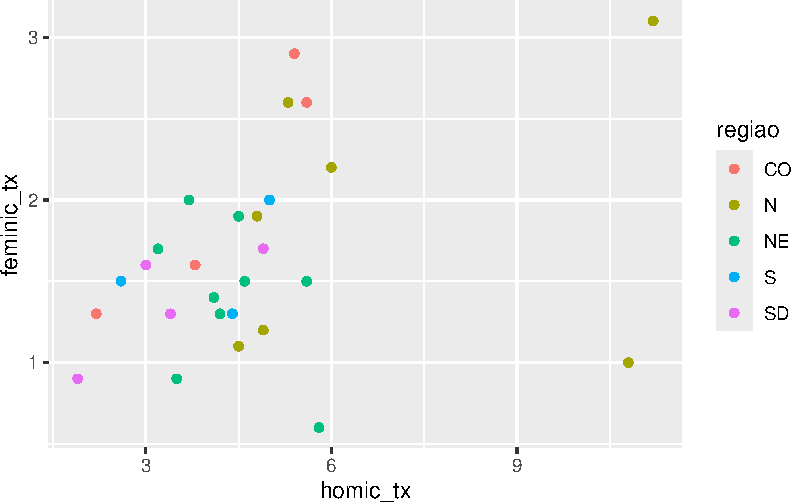
\includegraphics[keepaspectratio]{descritiva_v2_files/figure-pdf/unnamed-chunk-6-1.pdf}}

Ou podemos fazer que todos os pontos seja azul escuro:

\begin{Shaded}
\begin{Highlighting}[]
\FunctionTok{ggplot}\NormalTok{(}\AttributeTok{data =}\NormalTok{ final\_fem\_22, }\FunctionTok{aes}\NormalTok{(}\AttributeTok{x =}\NormalTok{ homic\_tx, }\AttributeTok{y =}\NormalTok{ feminic\_tx))}\SpecialCharTok{+}
  \FunctionTok{geom\_point}\NormalTok{(}\AttributeTok{color=}\StringTok{"darkblue"}\NormalTok{)}
\end{Highlighting}
\end{Shaded}

\pandocbounded{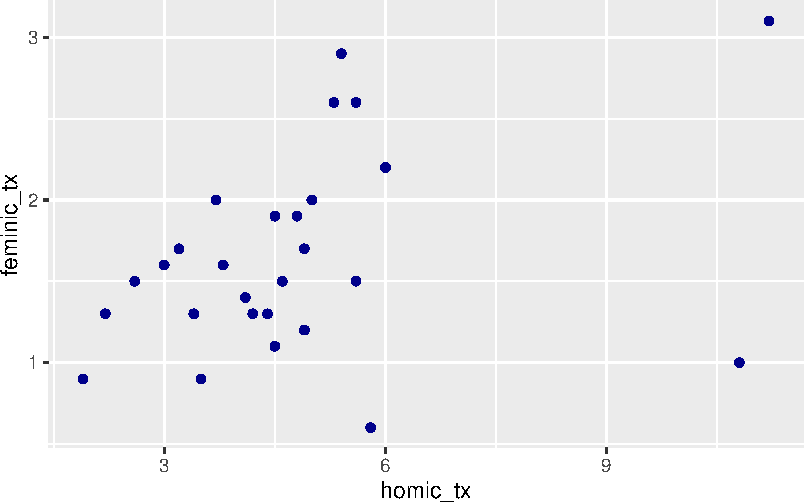
\includegraphics[keepaspectratio]{descritiva_v2_files/figure-pdf/unnamed-chunk-7-1.pdf}}

Para as cores uma possibilidade bem flexível é usar cores
\href{https://htmlcolorcodes.com/}{Hexadecimais}. Vamos usar a cor
\texttt{\#6e94bd} para os pontos:

Podemos mudar o tamanho \texttt{size}, a transparência com
\texttt{alpha} e a forma \texttt{shape} dos pontos:

\begin{Shaded}
\begin{Highlighting}[]
\FunctionTok{ggplot}\NormalTok{(}\AttributeTok{data =}\NormalTok{ final\_fem\_22, }\FunctionTok{aes}\NormalTok{(}\AttributeTok{x =}\NormalTok{ homic\_tx, }\AttributeTok{y =}\NormalTok{ feminic\_tx))}\SpecialCharTok{+}
  \FunctionTok{geom\_point}\NormalTok{(}\AttributeTok{color=}\StringTok{"\#6e94bd"}\NormalTok{, }\AttributeTok{size=}\DecValTok{3}\NormalTok{, }\AttributeTok{alpha=}\FloatTok{0.7}\NormalTok{,  }\AttributeTok{shape=}\DecValTok{17}\NormalTok{) }\SpecialCharTok{+}
  \FunctionTok{scale\_x\_continuous}\NormalTok{(}\AttributeTok{limits =} \FunctionTok{c}\NormalTok{(}\DecValTok{0}\NormalTok{, }\DecValTok{13}\NormalTok{))}
\end{Highlighting}
\end{Shaded}

\pandocbounded{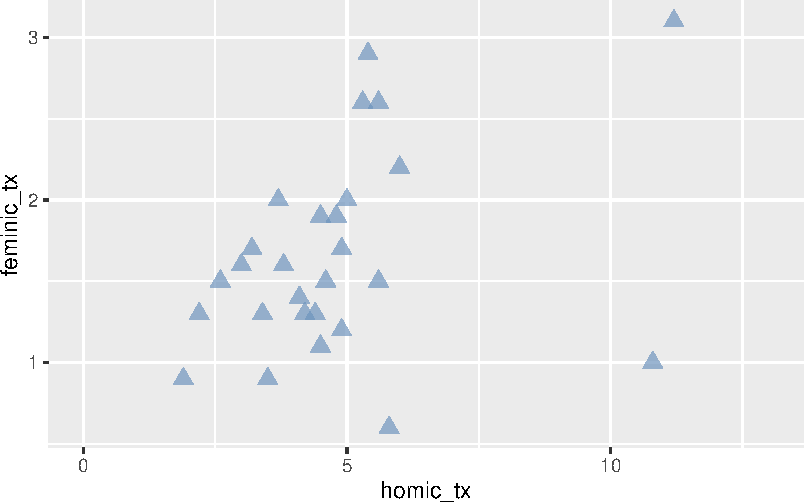
\includegraphics[keepaspectratio]{descritiva_v2_files/figure-pdf/unnamed-chunk-8-1.pdf}}

\begin{tcolorbox}[enhanced jigsaw, bottomrule=.15mm, leftrule=.75mm, arc=.35mm, colframe=quarto-callout-note-color-frame, breakable, opacityback=0, toprule=.15mm, colback=white, left=2mm, rightrule=.15mm]
\begin{minipage}[t]{5.5mm}
\textcolor{quarto-callout-note-color}{\faInfo}
\end{minipage}%
\begin{minipage}[t]{\textwidth - 5.5mm}

\vspace{-3mm}\textbf{Clique aqui para ver os \texttt{shapes} disponíveis}\vspace{3mm}

\begin{itemize}
\tightlist
\item
  \textbf{shape = 0}: quadrado\\
\item
  \textbf{shape = 1}: círculo\\
\item
  \textbf{shape = 2}: triângulo apontando para cima\\
\item
  \textbf{shape = 3}: sinal de mais (+)\\
\item
  \textbf{shape = 4}: cruz (x)\\
\item
  \textbf{shape = 5}: losango\\
\item
  \textbf{shape = 6}: triângulo apontando para baixo\\
\item
  \textbf{shape = 7}: quadrado com cruz\\
\item
  \textbf{shape = 8}: estrela\\
\item
  \textbf{shape = 9}: losango com sinal de mais\\
\item
  \textbf{shape = 10}: círculo com sinal de mais\\
\item
  \textbf{shape = 11}: triângulos apontando para cima e para baixo\\
\item
  \textbf{shape = 12}: quadrado com sinal de mais\\
\item
  \textbf{shape = 13}: círculo com cruz\\
\item
  \textbf{shape = 14}: quadrado com triângulo apontando para baixo\\
\item
  \textbf{shape = 15}: quadrado preenchido\\
\item
  \textbf{shape = 16}: círculo preenchido\\
\item
  \textbf{shape = 17}: triângulo preenchido apontando para cima\\
\item
  \textbf{shape = 18}: losango preenchido\\
\item
  \textbf{shape = 19}: círculo sólido\\
\item
  \textbf{shape = 20}: ponto (círculo menor)\\
\item
  \textbf{shape = 21}: círculo preenchido azul\\
\item
  \textbf{shape = 22}: quadrado preenchido azul\\
\item
  \textbf{shape = 23}: losango preenchido azul\\
\item
  \textbf{shape = 24}: triângulo preenchido apontando para cima azul\\
\item
  \textbf{shape = 25}: triângulo preenchido apontando para baixo azul
\end{itemize}

\end{minipage}%
\end{tcolorbox}

Agora vamos adicionar uma escala para o eixo de x entre 0 e 13 e vamos
dividir o gráfico por região:

\begin{Shaded}
\begin{Highlighting}[]
\FunctionTok{ggplot}\NormalTok{(}\AttributeTok{data =}\NormalTok{ final\_fem\_22, }\FunctionTok{aes}\NormalTok{(}\AttributeTok{x =}\NormalTok{ homic\_tx, }\AttributeTok{y =}\NormalTok{ feminic\_tx))}\SpecialCharTok{+}
  \FunctionTok{geom\_point}\NormalTok{(}\AttributeTok{color=}\StringTok{"\#6e94bd"}\NormalTok{, }\AttributeTok{size=}\DecValTok{3}\NormalTok{, }\AttributeTok{alpha=}\FloatTok{0.7}\NormalTok{,  }\AttributeTok{shape=}\DecValTok{17}\NormalTok{) }\SpecialCharTok{+}
  \FunctionTok{scale\_x\_continuous}\NormalTok{(}\AttributeTok{limits =} \FunctionTok{c}\NormalTok{(}\DecValTok{0}\NormalTok{, }\DecValTok{13}\NormalTok{))}\SpecialCharTok{+}
  \FunctionTok{facet\_wrap}\NormalTok{(}\SpecialCharTok{\textasciitilde{}}\NormalTok{regiao)}
\end{Highlighting}
\end{Shaded}

\pandocbounded{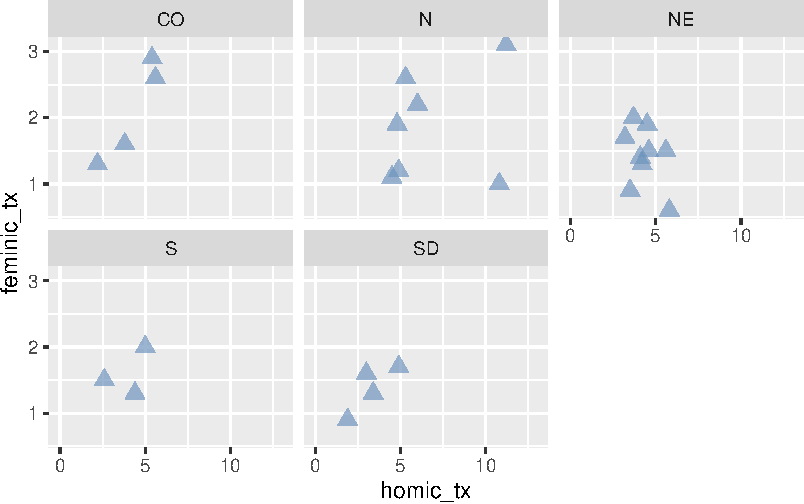
\includegraphics[keepaspectratio]{descritiva_v2_files/figure-pdf/unnamed-chunk-9-1.pdf}}

Pode-se também adicionar uma linha de tendência ao gráfico:

\begin{Shaded}
\begin{Highlighting}[]
\FunctionTok{ggplot}\NormalTok{(}\AttributeTok{data =}\NormalTok{ final\_fem\_22, }\FunctionTok{aes}\NormalTok{(}\AttributeTok{x =}\NormalTok{ homic\_tx, }\AttributeTok{y =}\NormalTok{ feminic\_tx))}\SpecialCharTok{+}
  \FunctionTok{geom\_point}\NormalTok{(}\AttributeTok{color=}\StringTok{"\#6e94bd"}\NormalTok{, }\AttributeTok{size=}\DecValTok{3}\NormalTok{, }\AttributeTok{alpha=}\FloatTok{0.7}\NormalTok{,  }\AttributeTok{shape=}\DecValTok{17}\NormalTok{) }\SpecialCharTok{+}
  \FunctionTok{scale\_x\_continuous}\NormalTok{(}\AttributeTok{limits =} \FunctionTok{c}\NormalTok{(}\DecValTok{0}\NormalTok{, }\DecValTok{13}\NormalTok{))}\SpecialCharTok{+}
  \FunctionTok{geom\_smooth}\NormalTok{(}\AttributeTok{method =} \StringTok{"lm"}\NormalTok{, }\AttributeTok{se=}\ConstantTok{FALSE}\NormalTok{ , }\AttributeTok{color=}\StringTok{"orange"}\NormalTok{)}\SpecialCharTok{+}
  \FunctionTok{facet\_wrap}\NormalTok{(}\SpecialCharTok{\textasciitilde{}}\NormalTok{regiao)}
\end{Highlighting}
\end{Shaded}

\pandocbounded{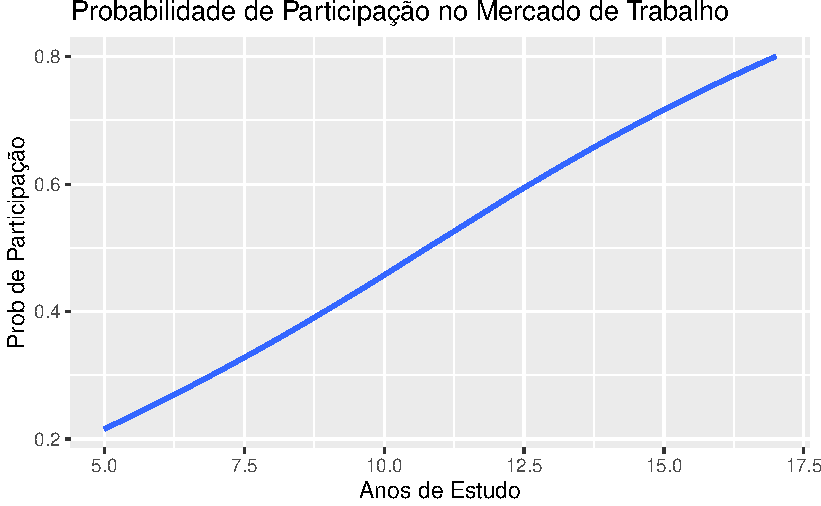
\includegraphics[keepaspectratio]{descritiva_v2_files/figure-pdf/unnamed-chunk-10-1.pdf}}

E por fim pode-se mudar o título e os rótulos dos eixos:

\begin{Shaded}
\begin{Highlighting}[]
\FunctionTok{library}\NormalTok{(ggthemes)}
\FunctionTok{ggplot}\NormalTok{(}\AttributeTok{data =}\NormalTok{ final\_fem\_22, }\FunctionTok{aes}\NormalTok{(}\AttributeTok{x =}\NormalTok{ homic\_tx, }\AttributeTok{y =}\NormalTok{ feminic\_tx))}\SpecialCharTok{+}
\FunctionTok{geom\_point}\NormalTok{(}\AttributeTok{color=}\StringTok{"\#6e94bd"}\NormalTok{, }\AttributeTok{size=}\DecValTok{3}\NormalTok{, }\AttributeTok{alpha=}\FloatTok{0.7}\NormalTok{,  }\AttributeTok{shape=}\DecValTok{17}\NormalTok{) }\SpecialCharTok{+}
\FunctionTok{scale\_x\_continuous}\NormalTok{(}\AttributeTok{limits =} \FunctionTok{c}\NormalTok{(}\DecValTok{0}\NormalTok{, }\DecValTok{13}\NormalTok{))}\SpecialCharTok{+}
\FunctionTok{geom\_smooth}\NormalTok{(}\AttributeTok{method =} \StringTok{"lm"}\NormalTok{, }\AttributeTok{se=}\ConstantTok{FALSE}\NormalTok{ , }\AttributeTok{color=}\StringTok{"orange"}\NormalTok{)}\SpecialCharTok{+}
\FunctionTok{facet\_wrap}\NormalTok{(}\SpecialCharTok{\textasciitilde{}}\NormalTok{regiao)}\SpecialCharTok{+}  
\FunctionTok{labs}\NormalTok{(}\AttributeTok{title=}\StringTok{"Homicídios e Feminicídios por Região"}\NormalTok{, }\AttributeTok{x=}\StringTok{"Homicídios"}\NormalTok{, }\AttributeTok{y=}\StringTok{"Feminicídios"}\NormalTok{)}\SpecialCharTok{+}
\FunctionTok{theme\_bw}\NormalTok{()}
\end{Highlighting}
\end{Shaded}

\pandocbounded{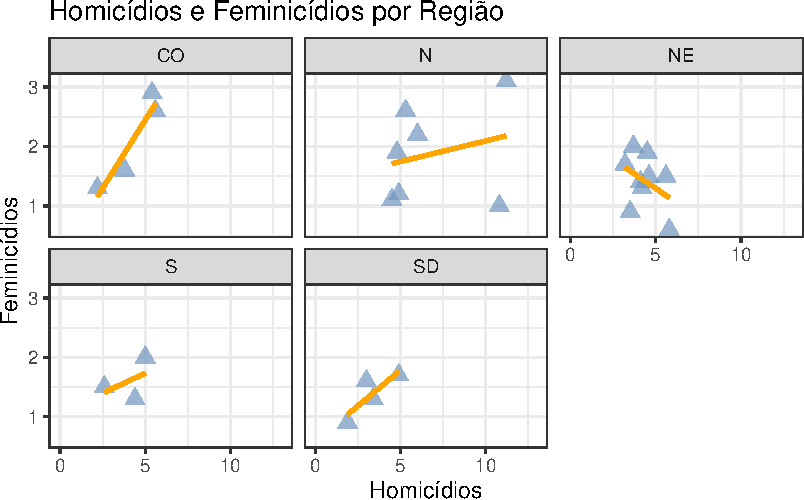
\includegraphics[keepaspectratio]{descritiva_v2_files/figure-pdf/unnamed-chunk-11-1.pdf}}

Para os temas pode acessar a
\href{https://r-graph-gallery.com/package/ggthemes.html}{Galeria} ou
\href{https://r-graph-gallery.com/ggplot2-package.html\#theme-widget}{Exemplos
Dinâmicos}.

\section{Medidas de Posição:}\label{medidas-de-posiuxe7uxe3o}

\textbf{MÉDIA AMOSTRAL:}

\[\bar{x} = \frac{1}{n} \sum_{i=1}^{n} x_i\]

\begin{Shaded}
\begin{Highlighting}[]
\FunctionTok{mean}\NormalTok{(final\_fem\_22}\SpecialCharTok{$}\NormalTok{feminic\_tx)}
\end{Highlighting}
\end{Shaded}

\begin{verbatim}
[1] 1.651852
\end{verbatim}

A média da taxa de Feminicídio entre os Estados do Brasil é de 1,65 por
100 mil mulheres em 2022 .

\begin{Shaded}
\begin{Highlighting}[]
\FunctionTok{library}\NormalTok{(kableExtra)}

\NormalTok{mean\_1}\OtherTok{\textless{}{-}} \FunctionTok{aggregate}\NormalTok{(final\_fem\_22[}\DecValTok{4}\SpecialCharTok{:}\DecValTok{15}\NormalTok{], }\FunctionTok{list}\NormalTok{(final\_fem\_22}\SpecialCharTok{$}\NormalTok{regiao), mean,  }\AttributeTok{na.rm=}\NormalTok{T)}

\FunctionTok{t}\NormalTok{(mean\_1) }\SpecialCharTok{\%\textgreater{}\%} 
  \FunctionTok{kbl}\NormalTok{(}\AttributeTok{digits =} \DecValTok{2}\NormalTok{) }\SpecialCharTok{\%\textgreater{}\%}
     \FunctionTok{kable\_styling}\NormalTok{()}
\end{Highlighting}
\end{Shaded}

\begin{table}
\centering
\begin{tabular}[t]{l|l|l|l|l|l}
\hline
Group.1 & CO & N & NE & S & SD\\
\hline
homic\_abs & 86.25000 & 69.85714 & 149.11111 & 212.66667 & 277.50000\\
\hline
homic\_tx & 4.250000 & 6.785714 & 4.355556 & 4.000000 & 3.300000\\
\hline
feminic\_abs & 40.50000 & 18.57143 & 43.55556 & 81.00000 & 127.50000\\
\hline
feminic\_tx & 2.100000 & 1.871429 & 1.422222 & 1.600000 & 1.375000\\
\hline
part\_feminic & 50.02500 & 30.01429 & 34.36667 & 41.53333 & 43.82500\\
\hline
rendapc & 2011.250 & 1175.286 & 1053.222 & 1983.667 & 1842.750\\
\hline
mais\_50 & 0.5000000 & 0.1428571 & 0.2222222 & 0.3333333 & 0.2500000\\
\hline
t\_homic\_abs & 258.2500 & 161.7143 & 257.7778 & 450.6667 & 455.7500\\
\hline
t\_homic\_tx & 13.375000 & 24.657143 & 9.311111 & 8.966667 & 8.875000\\
\hline
t\_feminic\_abs & 126.33333 & 50.28571 & 85.11111 & 169.66667 & 185.66667\\
\hline
t\_feminic\_tx & 6.500000 & 5.285714 & 3.044444 & 3.500000 & 3.000000\\
\hline
part\_t\_feminic & 32.67667 & 26.44286 & 25.72444 & 25.98667 & 26.50000\\
\hline
\end{tabular}
\end{table}

\textbf{MEDIANA:}

Organize os dados em ordem crescente.

\begin{enumerate}
\def\labelenumi{\alph{enumi})}
\item
  Para um numero impar de observações a mediana é o valor que ocupa a
  posição central.
\item
  para um número par de observações, a mediana é a média dos dois
  valores centrais.
\end{enumerate}

\begin{Shaded}
\begin{Highlighting}[]
\FunctionTok{median}\NormalTok{(final\_fem\_22}\SpecialCharTok{$}\NormalTok{feminic\_tx)}
\end{Highlighting}
\end{Shaded}

\begin{verbatim}
[1] 1.5
\end{verbatim}

Veja que a mediana é um valor diferente da média. Elas medem coisas
diferentes. Veja o exemplo abaixo

\begin{Shaded}
\begin{Highlighting}[]
\FunctionTok{median}\NormalTok{(}\FunctionTok{c}\NormalTok{(}\DecValTok{1}\NormalTok{,}\DecValTok{3}\NormalTok{, }\DecValTok{14}\NormalTok{))}
\end{Highlighting}
\end{Shaded}

\begin{verbatim}
[1] 3
\end{verbatim}

\begin{Shaded}
\begin{Highlighting}[]
\FunctionTok{mean}\NormalTok{(}\FunctionTok{c}\NormalTok{(}\DecValTok{1}\NormalTok{,}\DecValTok{3}\NormalTok{, }\DecValTok{14}\NormalTok{))}
\end{Highlighting}
\end{Shaded}

\begin{verbatim}
[1] 6
\end{verbatim}

Mediana e média são bastante distintas. Vamos fazer uma tabela com a
Média e Mediana, para o nosso conjunto de dados.

\begin{Shaded}
\begin{Highlighting}[]
\NormalTok{fun1 }\OtherTok{\textless{}{-}} \ControlFlowTok{function}\NormalTok{(x, }\AttributeTok{na.rm =} \ConstantTok{TRUE}\NormalTok{) }\FunctionTok{c}\NormalTok{(Média}\OtherTok{=}\FunctionTok{mean}\NormalTok{(x, }\AttributeTok{na.rm =} \ConstantTok{TRUE}\NormalTok{), }\AttributeTok{Mediana=}\FunctionTok{median}\NormalTok{(x, }\AttributeTok{na.rm =} \ConstantTok{TRUE}\NormalTok{))}

\NormalTok{median\_1 }\OtherTok{\textless{}{-}}\NormalTok{ (}\FunctionTok{sapply}\NormalTok{(final\_fem\_22[}\DecValTok{4}\SpecialCharTok{:}\DecValTok{15}\NormalTok{], fun1))}

\FunctionTok{t}\NormalTok{(median\_1) }\SpecialCharTok{\%\textgreater{}\%} 
  \FunctionTok{kbl}\NormalTok{(}\AttributeTok{digits =} \DecValTok{2}\NormalTok{) }\SpecialCharTok{\%\textgreater{}\%}
     \FunctionTok{kable\_styling}\NormalTok{()}
\end{Highlighting}
\end{Shaded}

\begin{table}
\centering
\begin{tabular}[t]{l|r|r}
\hline
  & Média & Mediana\\
\hline
homic\_abs & 145.33 & 95.00\\
\hline
homic\_tx & 4.77 & 4.50\\
\hline
feminic\_abs & 53.22 & 33.00\\
\hline
feminic\_tx & 1.65 & 1.50\\
\hline
part\_feminic & 37.76 & 38.90\\
\hline
rendapc & 1447.15 & 1267.00\\
\hline
mais\_50 & 0.26 & 0.00\\
\hline
t\_homic\_abs & 283.70 & 264.00\\
\hline
t\_homic\_tx & 13.79 & 10.00\\
\hline
t\_feminic\_abs & 102.52 & 88.00\\
\hline
t\_feminic\_tx & 4.14 & 3.60\\
\hline
part\_t\_feminic & 26.88 & 29.73\\
\hline
\end{tabular}
\end{table}

\textbf{MODA:}

Moda é o valor que ocorre com mais frequência.

\begin{Shaded}
\begin{Highlighting}[]
\NormalTok{moda }\OtherTok{\textless{}{-}} \ControlFlowTok{function}\NormalTok{(x, }\AttributeTok{na.rm=}\NormalTok{T) \{}
\NormalTok{modal }\OtherTok{\textless{}{-}} \FunctionTok{unique}\NormalTok{(x, }\AttributeTok{na.rm=}\NormalTok{T)}
\NormalTok{modal[}\FunctionTok{which.max}\NormalTok{(}\FunctionTok{tabulate}\NormalTok{(}\FunctionTok{match}\NormalTok{(x, modal)))]}
\NormalTok{\}}
\FunctionTok{moda}\NormalTok{(final\_fem\_22}\SpecialCharTok{$}\NormalTok{feminic\_tx)}
\end{Highlighting}
\end{Shaded}

\begin{verbatim}
[1] 1.3
\end{verbatim}

\begin{Shaded}
\begin{Highlighting}[]
\NormalTok{fun1 }\OtherTok{\textless{}{-}} \ControlFlowTok{function}\NormalTok{(x, }\AttributeTok{na.rm =} \ConstantTok{TRUE}\NormalTok{) }\FunctionTok{c}\NormalTok{(Média}\OtherTok{=}\FunctionTok{mean}\NormalTok{(x, }\AttributeTok{na.rm =} \ConstantTok{TRUE}\NormalTok{), }\AttributeTok{Mediana=}\FunctionTok{median}\NormalTok{(x, }\AttributeTok{na.rm =} \ConstantTok{TRUE}\NormalTok{), }\AttributeTok{Moda=}\FunctionTok{moda}\NormalTok{(x))}

\NormalTok{median\_1 }\OtherTok{\textless{}{-}}\NormalTok{ (}\FunctionTok{sapply}\NormalTok{(final\_fem\_22[}\DecValTok{4}\SpecialCharTok{:}\DecValTok{15}\NormalTok{], fun1))}

\FunctionTok{t}\NormalTok{(median\_1) }\SpecialCharTok{\%\textgreater{}\%} 
  \FunctionTok{kbl}\NormalTok{(}\AttributeTok{digits =} \DecValTok{2}\NormalTok{) }\SpecialCharTok{\%\textgreater{}\%}
     \FunctionTok{kable\_styling}\NormalTok{()}
\end{Highlighting}
\end{Shaded}

\begin{table}
\centering
\begin{tabular}[t]{l|r|r|r}
\hline
  & Média & Mediana & Moda\\
\hline
homic\_abs & 145.33 & 95.00 & 22.0\\
\hline
homic\_tx & 4.77 & 4.50 & 4.5\\
\hline
feminic\_abs & 53.22 & 33.00 & 19.0\\
\hline
feminic\_tx & 1.65 & 1.50 & 1.3\\
\hline
part\_feminic & 37.76 & 38.90 & 50.0\\
\hline
rendapc & 1447.15 & 1267.00 & 1010.0\\
\hline
mais\_50 & 0.26 & 0.00 & 0.0\\
\hline
t\_homic\_abs & 283.70 & 264.00 & 373.0\\
\hline
t\_homic\_tx & 13.79 & 10.00 & 4.2\\
\hline
t\_feminic\_abs & 102.52 & 88.00 & 54.0\\
\hline
t\_feminic\_tx & 4.14 & 3.60 & 2.3\\
\hline
part\_t\_feminic & 26.88 & 29.73 & NA\\
\hline
\end{tabular}
\end{table}

\subsubsection{Visualizando as medidas por
categorias}\label{visualizando-as-medidas-por-categorias}

\textbf{Gráfico de Pizza}

O gráfico de pizza indica as proporções de uma determinada variável de
classe. Aqui utilizamos a média do número de feminicídios absoluto por
região.

\begin{Shaded}
\begin{Highlighting}[]
\FunctionTok{ggplot}\NormalTok{(mean\_1, }\FunctionTok{aes}\NormalTok{(}\AttributeTok{x =} \StringTok{""}\NormalTok{, }\AttributeTok{y =}\NormalTok{ feminic\_abs, }\AttributeTok{fill =}\NormalTok{ Group}\FloatTok{.1}\NormalTok{)) }\SpecialCharTok{+}
  \FunctionTok{geom\_col}\NormalTok{(}\AttributeTok{width =} \DecValTok{1}\NormalTok{, }\AttributeTok{color =} \StringTok{"lightgray"}\NormalTok{) }\SpecialCharTok{+}
  \FunctionTok{coord\_polar}\NormalTok{(}\AttributeTok{theta =} \StringTok{"y"}\NormalTok{) }\SpecialCharTok{+}
  \FunctionTok{labs}\NormalTok{(}\AttributeTok{title =} \StringTok{"Média Feminicídio por Região"}\NormalTok{, }\AttributeTok{fill =} \StringTok{"Região"}\NormalTok{) }\SpecialCharTok{+}
  \FunctionTok{theme\_minimal}\NormalTok{() }\SpecialCharTok{+}
  \FunctionTok{theme}\NormalTok{(}\AttributeTok{axis.title =} \FunctionTok{element\_blank}\NormalTok{(),}
        \AttributeTok{axis.text =} \FunctionTok{element\_blank}\NormalTok{(),}
        \AttributeTok{axis.ticks =} \FunctionTok{element\_blank}\NormalTok{())}\SpecialCharTok{+} 
  \FunctionTok{scale\_fill\_brewer}\NormalTok{(}\AttributeTok{palette=}\StringTok{"PuBu"}\NormalTok{)}
\end{Highlighting}
\end{Shaded}

\pandocbounded{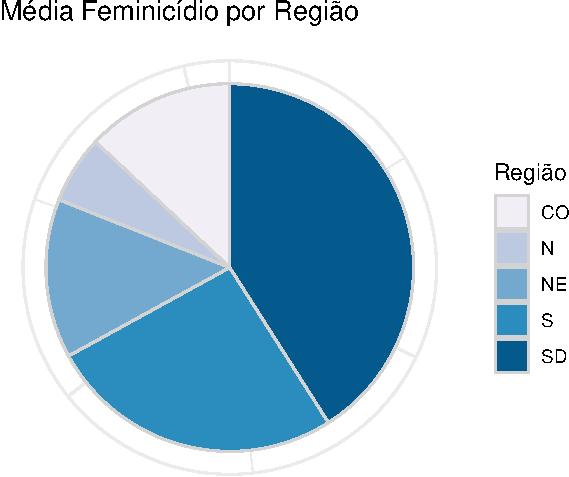
\includegraphics[keepaspectratio]{descritiva_v2_files/figure-pdf/unnamed-chunk-19-1.pdf}}

\begin{tcolorbox}[enhanced jigsaw, leftrule=.75mm, coltitle=black, colframe=quarto-callout-tip-color-frame, toprule=.15mm, opacitybacktitle=0.6, bottomtitle=1mm, bottomrule=.15mm, titlerule=0mm, toptitle=1mm, title=\textcolor{quarto-callout-tip-color}{\faLightbulb}\hspace{0.5em}{Exercício}, arc=.35mm, breakable, opacityback=0, colbacktitle=quarto-callout-tip-color!10!white, colback=white, left=2mm, rightrule=.15mm]

\textbf{PERGUNTA}: Qual a proporção de estados que possuem taxas de
feminicídio acima de 50\%?

\end{tcolorbox}

\begin{tcolorbox}[enhanced jigsaw, bottomrule=.15mm, leftrule=.75mm, arc=.35mm, colframe=quarto-callout-warning-color-frame, breakable, opacityback=0, toprule=.15mm, colback=white, left=2mm, rightrule=.15mm]
\begin{minipage}[t]{5.5mm}
\textcolor{quarto-callout-warning-color}{\faExclamationTriangle}
\end{minipage}%
\begin{minipage}[t]{\textwidth - 5.5mm}

\vspace{-3mm}\textbf{Veja a Resposta}\vspace{3mm}

\textbf{RESPOSTA}: Participação é uma variável disecreta do tipo 0 ou 1
(binárias) que indica se a taxa de feminicídio é maior que 50\%.

\begin{Shaded}
\begin{Highlighting}[]
\FunctionTok{library}\NormalTok{(dplyr)}
\NormalTok{final\_fem\_22 }\SpecialCharTok{|\textgreater{}} 
  \FunctionTok{group\_by}\NormalTok{(mais\_50) }\SpecialCharTok{|\textgreater{}}
  \FunctionTok{summarise}\NormalTok{(}\AttributeTok{cont =} \FunctionTok{n}\NormalTok{()) }\SpecialCharTok{|\textgreater{}} 
  \FunctionTok{mutate}\NormalTok{(}\AttributeTok{mais\_50F =} \FunctionTok{factor}\NormalTok{(mais\_50, }\AttributeTok{levels =} \FunctionTok{c}\NormalTok{(}\DecValTok{0}\NormalTok{, }\DecValTok{1}\NormalTok{), }\AttributeTok{labels =} \FunctionTok{c}\NormalTok{(}\StringTok{"Abaixo de 50\%"}\NormalTok{, }\StringTok{"Acima de 50\%"}\NormalTok{))) }\SpecialCharTok{|\textgreater{}} 
  \FunctionTok{ggplot}\NormalTok{( }\FunctionTok{aes}\NormalTok{(}\AttributeTok{x=}\StringTok{""}\NormalTok{, }\AttributeTok{y =}\NormalTok{cont, }\AttributeTok{fill=}\NormalTok{mais\_50F)) }\SpecialCharTok{+}
  \FunctionTok{geom\_bar}\NormalTok{(}\AttributeTok{stat=}\StringTok{"identity"}\NormalTok{, }\AttributeTok{width =} \DecValTok{1}\NormalTok{, }\AttributeTok{color =} \StringTok{"lightgray"}\NormalTok{) }\SpecialCharTok{+}
  \FunctionTok{coord\_polar}\NormalTok{(}\AttributeTok{theta =} \StringTok{"y"}\NormalTok{, }\AttributeTok{start=}\DecValTok{0}\NormalTok{)}\SpecialCharTok{+}
  \FunctionTok{labs}\NormalTok{(}\AttributeTok{title =} \StringTok{"Participação do Feminicídio no Total de Homicídios Femininos"}\NormalTok{, }\AttributeTok{fill =} \StringTok{"Participação Feminicídio"}\NormalTok{) }\SpecialCharTok{+}
  \FunctionTok{theme\_minimal}\NormalTok{() }\SpecialCharTok{+}
  \FunctionTok{theme}\NormalTok{(}\AttributeTok{axis.title =} \FunctionTok{element\_blank}\NormalTok{(),}
        \AttributeTok{axis.text =} \FunctionTok{element\_blank}\NormalTok{(),}
        \AttributeTok{axis.ticks =} \FunctionTok{element\_blank}\NormalTok{())}\SpecialCharTok{+}
  \FunctionTok{scale\_fill\_brewer}\NormalTok{(}\AttributeTok{palette=}\StringTok{"Blues"}\NormalTok{)}
\end{Highlighting}
\end{Shaded}

\pandocbounded{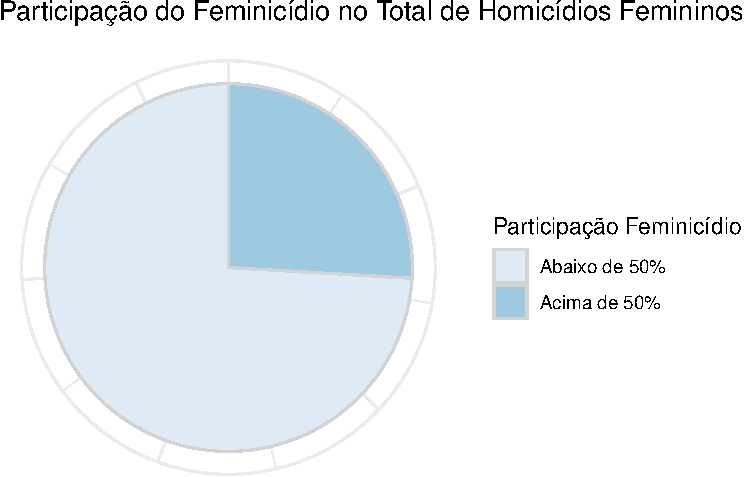
\includegraphics[keepaspectratio]{descritiva_v2_files/figure-pdf/unnamed-chunk-21-1.pdf}}

\end{minipage}%
\end{tcolorbox}

\textbf{Gráfico de Barra}

Em geral a utilização do gráfico de barras está relacionado ao
entendimento da frequência de valores associados a uma determinada
categoria. Por exemplo, imagine que temos um banco de dados com as
pessoas classificadas como: i)Não trabalha; ii)Trabalha e
iii)Desempregado. Teríamos três categorias e a frequência de pessoas em
cada categoria. Poderíamos ainda dividir essa categoria entre homens e
mulheres. Essa é a utilização mais padrão do gráfico de barras. Vejamos
alguns gráficos:

\begin{Shaded}
\begin{Highlighting}[]
\FunctionTok{ggplot}\NormalTok{(final\_fem\_22, }\FunctionTok{aes}\NormalTok{(}\AttributeTok{x =} \FunctionTok{reorder}\NormalTok{(estados, }\SpecialCharTok{{-}}\NormalTok{feminic\_tx), }\AttributeTok{y =}\NormalTok{ feminic\_tx)) }\SpecialCharTok{+}
  \FunctionTok{geom\_bar}\NormalTok{(}\AttributeTok{stat =} \StringTok{"identity"}\NormalTok{, }\AttributeTok{fill =} \StringTok{"salmon2"}\NormalTok{, }\AttributeTok{alpha=}\FloatTok{0.5}\NormalTok{, }\AttributeTok{color =} \StringTok{"lightsalmon4"}\NormalTok{) }\SpecialCharTok{+}
  \FunctionTok{labs}\NormalTok{(}\AttributeTok{title =} \StringTok{"Taxa de Feminicídio por Estado"}\NormalTok{,}
       \AttributeTok{x =} \StringTok{""}\NormalTok{,}
       \AttributeTok{y =} \StringTok{"Tx. por 100 mil"}\NormalTok{) }\SpecialCharTok{+}
  \FunctionTok{theme\_minimal}\NormalTok{() }\SpecialCharTok{+}
  \FunctionTok{theme}\NormalTok{(}\AttributeTok{axis.text.x =} \FunctionTok{element\_text}\NormalTok{(}\AttributeTok{angle =} \DecValTok{90}\NormalTok{, }\AttributeTok{vjust =} \FloatTok{0.5}\NormalTok{, }\AttributeTok{hjust =} \DecValTok{1}\NormalTok{, }\AttributeTok{size =} \DecValTok{9}\NormalTok{)) }
\end{Highlighting}
\end{Shaded}

\pandocbounded{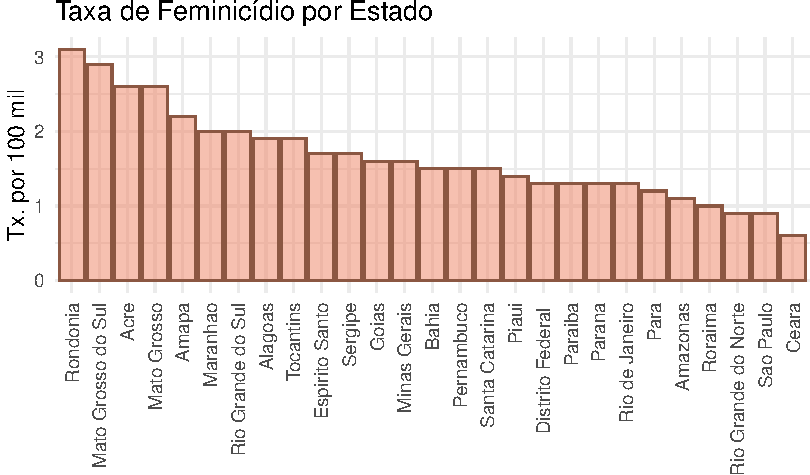
\includegraphics[keepaspectratio]{descritiva_v2_files/figure-pdf/unnamed-chunk-22-1.pdf}}

Vamos fazer um gráfico de barras para a participação do Feminicídio no
total de homicídios femininos por Estado.

\begin{Shaded}
\begin{Highlighting}[]
\FunctionTok{ggplot}\NormalTok{(final\_fem\_22, }\FunctionTok{aes}\NormalTok{(}\AttributeTok{x =} \FunctionTok{reorder}\NormalTok{(estados, }\SpecialCharTok{{-}}\NormalTok{part\_feminic), }\AttributeTok{y =}\NormalTok{ part\_feminic)) }\SpecialCharTok{+} \CommentTok{\# Ordem decrescente}
  \FunctionTok{geom\_col}\NormalTok{( }\AttributeTok{fill =} \StringTok{"\#3f566f"}\NormalTok{, }\AttributeTok{alpha=}\FloatTok{0.7}\NormalTok{, }\AttributeTok{color =} \StringTok{"\#4c5471"}\NormalTok{) }\SpecialCharTok{+}                      \CommentTok{\# Adiciona as barras, cor das barras, transparencia }
  \FunctionTok{labs}\NormalTok{(                                                                            }\CommentTok{\# e cor da borda}
    \AttributeTok{title =} \StringTok{"Participação da Taxa de Feminicídio no Total por Estado"}\NormalTok{,             }\CommentTok{\# Título do gráfico}
    \AttributeTok{x =} \StringTok{""}\NormalTok{,                                                                        }\CommentTok{\# Rótulo do eixo x}
    \AttributeTok{y =} \StringTok{"Tx. por 100 mil"}                                                          \CommentTok{\# Rótulo do eixo y}
\NormalTok{  ) }\SpecialCharTok{+}
  \FunctionTok{theme\_bw}\NormalTok{() }\SpecialCharTok{+}
  \FunctionTok{theme}\NormalTok{(}\AttributeTok{axis.text.x =} \FunctionTok{element\_text}\NormalTok{(}\AttributeTok{angle =} \DecValTok{90}\NormalTok{, }\AttributeTok{hjust =} \DecValTok{1}\NormalTok{, }\AttributeTok{size =} \DecValTok{9}\NormalTok{))              }\CommentTok{\# Ajusta o tamanho do texto do eixo x}
\end{Highlighting}
\end{Shaded}

\pandocbounded{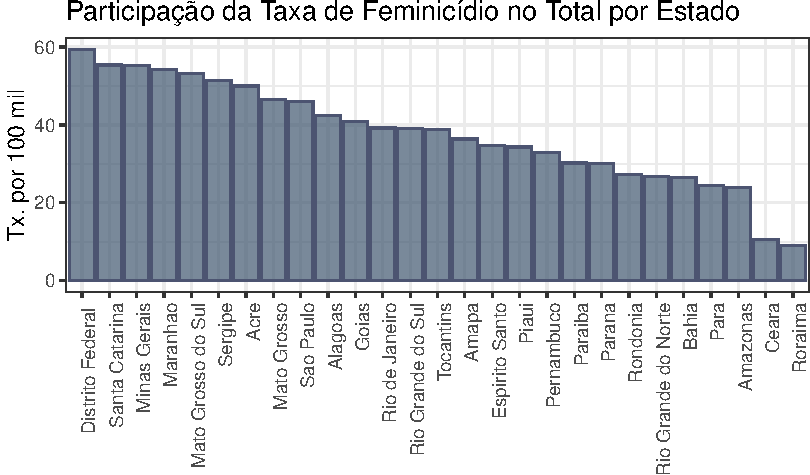
\includegraphics[keepaspectratio]{descritiva_v2_files/figure-pdf/unnamed-chunk-23-1.pdf}}

\textbf{Gráfico de Barras Agrupadas}

Vamos fazer um gráfico de barras agrupadas para a taxa de feminicídio e
taxa de tentativa de feminicídio por região. Vamos passo a passo:

\begin{enumerate}
\def\labelenumi{\arabic{enumi}.}
\tightlist
\item
  Transformar os dados em formato long
\end{enumerate}

\begin{Shaded}
\begin{Highlighting}[]
\FunctionTok{library}\NormalTok{(tidyr)}
\FunctionTok{library}\NormalTok{(dplyr)}

\CommentTok{\# Transformar os dados no formato long}
\NormalTok{tx\_long }\OtherTok{\textless{}{-}}\NormalTok{ final\_fem\_22 }\SpecialCharTok{\%\textgreater{}\%}
  \FunctionTok{arrange}\NormalTok{(}\FunctionTok{desc}\NormalTok{(feminic\_tx)) }\SpecialCharTok{\%\textgreater{}\%}                          \CommentTok{\# Ordena pelos valores de feinic\_tx, decrescente}
  \FunctionTok{select}\NormalTok{(estados, regiao, feminic\_tx, t\_feminic\_tx) }\SpecialCharTok{\%\textgreater{}\%}  \CommentTok{\# Seleciona as colunas de interesse}
  \FunctionTok{pivot\_longer}\NormalTok{(}\AttributeTok{cols =} \FunctionTok{c}\NormalTok{(feminic\_tx, t\_feminic\_tx),       }\CommentTok{\# Converte para formato longo}
               \AttributeTok{names\_to =} \StringTok{"tipo"}\NormalTok{,                        }\CommentTok{\# Nome da coluna que identificará as variáveis}
               \AttributeTok{values\_to =} \StringTok{"taxa"}\NormalTok{)                       }\CommentTok{\# Nome da coluna que armazenará os valores}

\FunctionTok{head}\NormalTok{(tx\_long)}
\end{Highlighting}
\end{Shaded}

\begin{verbatim}
# A tibble: 6 x 4
  estados            regiao tipo          taxa
  <chr>              <chr>  <chr>        <dbl>
1 Rondonia           N      feminic_tx     3.1
2 Rondonia           N      t_feminic_tx   2.9
3 Mato Grosso do Sul CO     feminic_tx     2.9
4 Mato Grosso do Sul CO     t_feminic_tx   8.8
5 Acre               N      feminic_tx     2.6
6 Acre               N      t_feminic_tx   3.9
\end{verbatim}

\begin{enumerate}
\def\labelenumi{\arabic{enumi}.}
\setcounter{enumi}{1}
\tightlist
\item
  Criar o gráfico de barras lado a lado
\end{enumerate}

\begin{Shaded}
\begin{Highlighting}[]
\CommentTok{\# Criar o gráfico de barras lado a lado}
\FunctionTok{ggplot}\NormalTok{(tx\_long, }\FunctionTok{aes}\NormalTok{(}\AttributeTok{x =} \FunctionTok{reorder}\NormalTok{(estados, }\SpecialCharTok{{-}}\NormalTok{taxa), }\AttributeTok{y =}\NormalTok{ taxa, }\AttributeTok{fill =}\NormalTok{ tipo)) }\SpecialCharTok{+}
  \FunctionTok{geom\_bar}\NormalTok{(}\AttributeTok{stat =} \StringTok{"identity"}\NormalTok{,}\AttributeTok{alpha=}\FloatTok{0.7}\NormalTok{,  }\AttributeTok{position =} \StringTok{"dodge"}\NormalTok{, }\AttributeTok{color =} \StringTok{"white"}\NormalTok{) }\SpecialCharTok{+}               \CommentTok{\# Barras lado a lado posição dodge faz isso}
  \FunctionTok{labs}\NormalTok{(}
    \AttributeTok{title =} \StringTok{"Comparação das Taxas de Feminicídio por Estado"}\NormalTok{,                     }\CommentTok{\# Título do gráfico}
    \AttributeTok{x =} \StringTok{""}\NormalTok{, }\CommentTok{\# Rótulo do eixo x                                                    \# Rótulo do eixo x, y e legenda}
    \AttributeTok{y =} \StringTok{"Tx. por 100 mil"}\NormalTok{,                                                        }
    \AttributeTok{fill =} \StringTok{"Tipo de Taxa"}                                                                
\NormalTok{  ) }\SpecialCharTok{+}
  \FunctionTok{scale\_fill\_manual}\NormalTok{(}
        \AttributeTok{values =} \FunctionTok{c}\NormalTok{(}\StringTok{"feminic\_tx"} \OtherTok{=} \StringTok{"\#7185cc"}\NormalTok{, }\StringTok{"t\_feminic\_tx"} \OtherTok{=} \StringTok{"\#c2986f"}\NormalTok{),              }\CommentTok{\# Definir as cores para cada variável}
        \AttributeTok{labels =} \FunctionTok{c}\NormalTok{(}\StringTok{"feminic\_tx"} \OtherTok{=} \StringTok{"Feminicídio"}\NormalTok{, }\StringTok{"t\_feminic\_tx"} \OtherTok{=} \StringTok{"Tentativa de Fem."}\NormalTok{) }\CommentTok{\# Definir os rótulos para cada variável}
\NormalTok{                    ) }\SpecialCharTok{+}  
  \FunctionTok{theme}\NormalTok{(}\AttributeTok{axis.text.x =} \FunctionTok{element\_text}\NormalTok{(}\AttributeTok{angle =} \DecValTok{90}\NormalTok{, }\AttributeTok{hjust =} \DecValTok{1}\NormalTok{, }\AttributeTok{size =} \DecValTok{8}\NormalTok{))                    }\CommentTok{\# Ajusta o tamanho do texto do eixo x}
\end{Highlighting}
\end{Shaded}

\pandocbounded{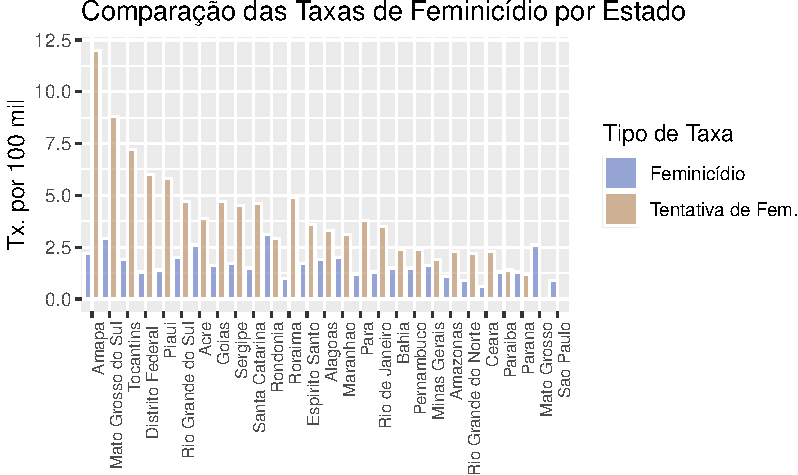
\includegraphics[keepaspectratio]{descritiva_v2_files/figure-pdf/unnamed-chunk-25-1.pdf}}

\textbf{Gráfico de Linha}

O gráfico de linha ou pontos é muito utilizado para visualização da
evolução de séries. É um gráfico que nos permite ver a evolução dos
salários entre homens e mulheres, evolução dos preços dos alimentos,
evolução do número de casos de feminicídio, evolução dos processos em
determinada Vara.

Nosso banco é uma fotografia e não uma evolução, o que torna esse tipo
de visualização menos útil. Vejamos a como a taxa de feminicídio evolui
com o aumento do número total Homicídios Femininos.

\begin{Shaded}
\begin{Highlighting}[]
\CommentTok{\# Ordenar os dados pelo número absoluto de homicídios do menor para o maior}
\NormalTok{final\_fem\_22 }\OtherTok{\textless{}{-}}\NormalTok{ final\_fem\_22[}\FunctionTok{order}\NormalTok{(}\SpecialCharTok{{-}}\NormalTok{final\_fem\_22}\SpecialCharTok{$}\NormalTok{homic\_abs),]}

\CommentTok{\# Criar o gráfico com ggplot2}
\FunctionTok{ggplot}\NormalTok{(final\_fem\_22, }\FunctionTok{aes}\NormalTok{(}\AttributeTok{x =}\NormalTok{ homic\_abs)) }\SpecialCharTok{+}
\CommentTok{\# Linha para \textquotesingle{}t\_feminic\_tx\textquotesingle{}}
  \FunctionTok{geom\_line}\NormalTok{(}\FunctionTok{aes}\NormalTok{(}\AttributeTok{y =}\NormalTok{ t\_feminic\_tx, }\AttributeTok{color =} \StringTok{"Tentativa"}\NormalTok{), }\AttributeTok{linewidth =} \FloatTok{0.8}\NormalTok{, }\AttributeTok{alpha=}\FloatTok{0.4}\NormalTok{) }\SpecialCharTok{+}
  \FunctionTok{geom\_point}\NormalTok{(}\FunctionTok{aes}\NormalTok{(}\AttributeTok{y =}\NormalTok{ t\_feminic\_tx, }\AttributeTok{color =} \StringTok{"Tentativa"}\NormalTok{), }\AttributeTok{size =} \DecValTok{3}\NormalTok{, }\AttributeTok{shape =} \DecValTok{17}\NormalTok{) }\SpecialCharTok{+}
\CommentTok{\# Linha para \textquotesingle{}feminic\_tx\textquotesingle{}}
  \FunctionTok{geom\_line}\NormalTok{(}\FunctionTok{aes}\NormalTok{(}\AttributeTok{y =}\NormalTok{ feminic\_tx, }\AttributeTok{color =} \StringTok{"Feminicídio"}\NormalTok{), }\AttributeTok{linewidth =} \FloatTok{0.8}\NormalTok{, }\AttributeTok{alpha=}\FloatTok{0.4}\NormalTok{) }\SpecialCharTok{+}
  \FunctionTok{geom\_point}\NormalTok{(}\FunctionTok{aes}\NormalTok{(}\AttributeTok{y =}\NormalTok{ feminic\_tx, }\AttributeTok{color =} \StringTok{"Feminicídio"}\NormalTok{), }\AttributeTok{size =} \DecValTok{3}\NormalTok{, }\AttributeTok{shape =} \DecValTok{19}\NormalTok{) }\SpecialCharTok{+}
\CommentTok{\# Escala de cores para as linhas}
  \FunctionTok{scale\_color\_manual}\NormalTok{(}
    \AttributeTok{values =} \FunctionTok{c}\NormalTok{(}\StringTok{"Tentativa"} \OtherTok{=} \StringTok{"\#c2986f"}\NormalTok{, }\StringTok{"Feminicídio"} \OtherTok{=} \StringTok{"\#7185cc"}\NormalTok{)}
\NormalTok{  ) }\SpecialCharTok{+}
\CommentTok{\# Títulos e rótulos}
  \FunctionTok{labs}\NormalTok{(}
    \AttributeTok{title =} \StringTok{"Tentativa e Feminicídio: Taxa"}\NormalTok{,}
    \AttributeTok{x =} \StringTok{"Total de Homicídios"}\NormalTok{,}
    \AttributeTok{y =} \StringTok{"Taxa / 100 mil"}\NormalTok{,}
    \AttributeTok{color =} \StringTok{"Tipo"}
\NormalTok{  ) }\SpecialCharTok{+}
 \CommentTok{\# Ajustes de tema}
  \FunctionTok{theme\_minimal}\NormalTok{() }\SpecialCharTok{+}
  \FunctionTok{theme}\NormalTok{(}
    \AttributeTok{plot.title =} \FunctionTok{element\_text}\NormalTok{(}\AttributeTok{hjust =} \FloatTok{0.5}\NormalTok{, }\AttributeTok{size =} \DecValTok{14}\NormalTok{, }\AttributeTok{face =} \StringTok{"bold"}\NormalTok{),  }\CommentTok{\# Centraliza o título, tamanho e negrito}
    \AttributeTok{legend.position =} \StringTok{"top"}\NormalTok{,                                           }\CommentTok{\# Posiciona a legenda no topo}
    \AttributeTok{legend.title =} \FunctionTok{element\_text}\NormalTok{(}\AttributeTok{size =} \DecValTok{10}\NormalTok{),                            }\CommentTok{\# Ajusta o tamanho do título da legenda}
    \AttributeTok{legend.text =} \FunctionTok{element\_text}\NormalTok{(}\AttributeTok{size =} \DecValTok{9}\NormalTok{)                               }\CommentTok{\# Ajusta o tamanho do texto da legenda}
\NormalTok{  )}
\end{Highlighting}
\end{Shaded}

\pandocbounded{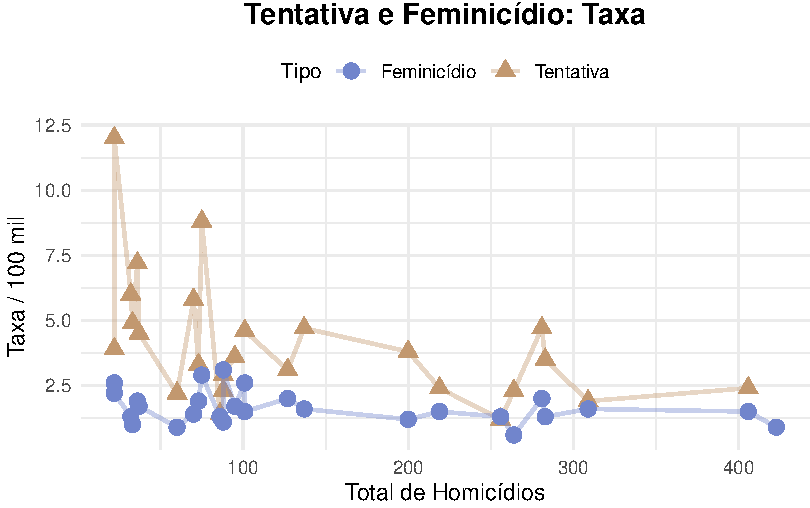
\includegraphics[keepaspectratio]{descritiva_v2_files/figure-pdf/unnamed-chunk-26-1.pdf}}

\begin{tcolorbox}[enhanced jigsaw, leftrule=.75mm, coltitle=black, colframe=quarto-callout-tip-color-frame, toprule=.15mm, opacitybacktitle=0.6, bottomtitle=1mm, bottomrule=.15mm, titlerule=0mm, toptitle=1mm, title=\textcolor{quarto-callout-tip-color}{\faLightbulb}\hspace{0.5em}{Exercício}, arc=.35mm, breakable, opacityback=0, colbacktitle=quarto-callout-tip-color!10!white, colback=white, left=2mm, rightrule=.15mm]

\textbf{PERGUNTA}: Será que quanto maior for a renda per capita, menor
será a taxa de feminicídio?

\end{tcolorbox}

\begin{tcolorbox}[enhanced jigsaw, bottomrule=.15mm, leftrule=.75mm, arc=.35mm, colframe=quarto-callout-warning-color-frame, breakable, opacityback=0, toprule=.15mm, colback=white, left=2mm, rightrule=.15mm]
\begin{minipage}[t]{5.5mm}
\textcolor{quarto-callout-warning-color}{\faExclamationTriangle}
\end{minipage}%
\begin{minipage}[t]{\textwidth - 5.5mm}

\vspace{-3mm}\textbf{Veja a Resposta}\vspace{3mm}

\textbf{RESPOSTA}: Renda e taxa de feminicídio são variáveis continuas.
O ideal seria utilizar um gráfico de dispersão para verificar a relação
entre essas variáveis.

\begin{Shaded}
\begin{Highlighting}[]
\FunctionTok{ggplot}\NormalTok{(}\AttributeTok{data =}\NormalTok{ final\_fem\_22, }\FunctionTok{aes}\NormalTok{(}\AttributeTok{x =}\NormalTok{ rendapc, }\AttributeTok{y =}\NormalTok{ feminic\_tx))}\SpecialCharTok{+}
\FunctionTok{geom\_point}\NormalTok{(}\AttributeTok{color=}\StringTok{"\#6e94bd"}\NormalTok{, }\AttributeTok{size=}\DecValTok{3}\NormalTok{, }\AttributeTok{alpha=}\FloatTok{0.7}\NormalTok{,  }\AttributeTok{shape=}\DecValTok{17}\NormalTok{) }\SpecialCharTok{+}
\FunctionTok{geom\_smooth}\NormalTok{(}\AttributeTok{method =} \StringTok{"lm"}\NormalTok{, }\AttributeTok{se=}\ConstantTok{TRUE}\NormalTok{ , }\AttributeTok{color=}\StringTok{"orange"}\NormalTok{)}\SpecialCharTok{+}
\FunctionTok{labs}\NormalTok{(}\AttributeTok{title=}\StringTok{"Renda pc e taxa de Feminicídios por Estado"}\NormalTok{, }\AttributeTok{x=}\StringTok{"Renda pc"}\NormalTok{, }\AttributeTok{y=}\StringTok{"Tx 100 mil"}\NormalTok{)}\SpecialCharTok{+}
\FunctionTok{theme\_bw}\NormalTok{()}
\end{Highlighting}
\end{Shaded}

\pandocbounded{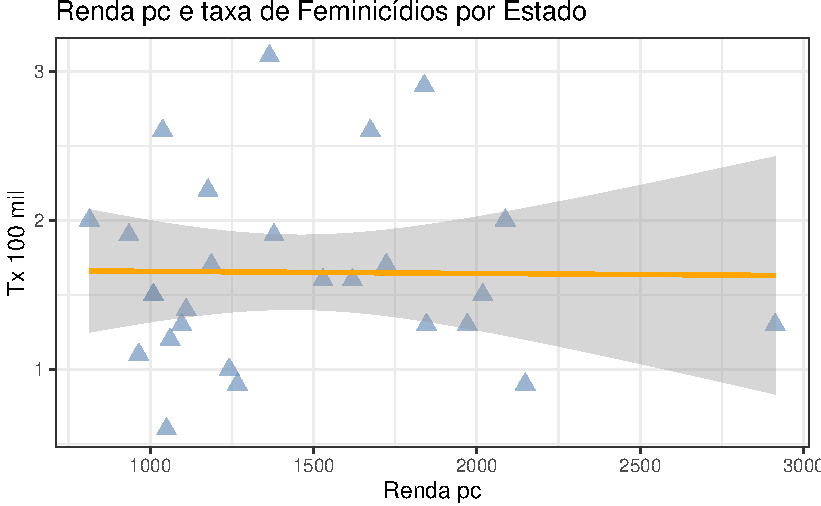
\includegraphics[keepaspectratio]{descritiva_v2_files/figure-pdf/unnamed-chunk-27-1.pdf}}

\end{minipage}%
\end{tcolorbox}

\textbf{PERCENTIL:}

O p-esimo percentil é um valor tal que ao menos p por cento das
observações são menores ou iguais à ele e pelo menos (100-p) por cento
das observações são maiores ou iguais a esse valor.

\emph{Etapas para calcular o p-ésimo percentil}

\textbf{Etapa 1}: Organize os dados em ordem crescente.

\textbf{Etapa 2}: Calcule um indice, \(i\) tal que
\[i = \frac{p}{100} \times n\] onde \(p\) é o percentil procurado

\textbf{Etapa 3}:

\begin{enumerate}
\def\labelenumi{\alph{enumi})}
\tightlist
\item
  Se \(i\) não for um número inteiro, arredondeo-o para cima. O próximo
  número inteiro maior que \(i\) denota a posição do p-esimo percentil.
\item
  Se \(i\) for um número inteiro o p-esimo percentil será a média dos
  valores que o ocupam as posições \(i\) e \(i + 1\).
\end{enumerate}

\begin{Shaded}
\begin{Highlighting}[]
\FunctionTok{quantile}\NormalTok{(final\_fem\_22}\SpecialCharTok{$}\NormalTok{feminic\_tx, }\AttributeTok{probs =} \FunctionTok{c}\NormalTok{(}\FloatTok{0.10}\NormalTok{,}\FloatTok{0.30}\NormalTok{,}\FloatTok{0.60}\NormalTok{,}\FloatTok{0.85}\NormalTok{), }\AttributeTok{na.rm=}\NormalTok{T)}
\end{Highlighting}
\end{Shaded}

\begin{verbatim}
 10%  30%  60%  85% 
0.96 1.30 1.66 2.24 
\end{verbatim}

\textbf{QUARTIS:}

Os quartis são medidas estatísticas que dividem um conjunto de dados
ordenados em quatro partes iguais. É um caso particular do percentil.

O três quartis são:

\textbf{Primeiro Quartil (Q1)}: Representa o valor abaixo do qual está
situada a primeira quarta parte (ou 25\% inferiores) dos dados quando
eles estão ordenados em ordem crescente. O primeiro quartil é o valor
que divide os dados em 25\% (ou 0.25) abaixo e 75\% (ou 0.75) acima
desse ponto.

\textbf{Segundo Quartil (Q2)}: Corresponde à mediana dos dados,
dividindo o conjunto em duas metades iguais. É o valor que separa os
50\% inferiores dos 50\% superiores dos dados.

\textbf{Terceiro Quartil (Q3)}: Indica o valor acima do qual está
situada a terceira quarta parte (ou 25\% superiores) dos dados quando
eles estão ordenados. Assim como o primeiro quartil, o terceiro quartil
divide os dados em 75\% (ou 0.75) abaixo e 25\% (ou 0.25) acima desse
ponto

\begin{Shaded}
\begin{Highlighting}[]
\FunctionTok{quantile}\NormalTok{(final\_fem\_22}\SpecialCharTok{$}\NormalTok{feminic\_tx, }\AttributeTok{na.rm=}\NormalTok{T)}
\end{Highlighting}
\end{Shaded}

\begin{verbatim}
  0%  25%  50%  75% 100% 
0.60 1.30 1.50 1.95 3.10 
\end{verbatim}

\section{Medidas de Variabilidade}\label{medidas-de-variabilidade}

\textbf{AMPLITUDE:}

Amplitude é a diferença entre o valor mínimo e máximo de uma série de
dados.

\[\text{Amplitude} = \text{Maior Valor} - \text{Menor Valor}\]

\begin{Shaded}
\begin{Highlighting}[]
\NormalTok{min\_max}\OtherTok{\textless{}{-}}\FunctionTok{range}\NormalTok{(final\_fem\_22}\SpecialCharTok{$}\NormalTok{feminic\_tx)}
\NormalTok{amp}\OtherTok{\textless{}{-}}\NormalTok{min\_max[}\DecValTok{2}\NormalTok{]}\SpecialCharTok{{-}}\NormalTok{min\_max[}\DecValTok{1}\NormalTok{]}
\NormalTok{amp}
\end{Highlighting}
\end{Shaded}

\begin{verbatim}
[1] 2.5
\end{verbatim}

\textbf{AMPLITUDE INTERQUANTIL:}

A amplitude interquartil é dada pela diferenca entre o terceiro
(\(Q_3\)) e o primeiro quartil (\(Q_1\)).

\[IQR = Q_3 - Q_1\]

\begin{Shaded}
\begin{Highlighting}[]
\NormalTok{qs}\OtherTok{\textless{}{-}}\FunctionTok{quantile}\NormalTok{(final\_fem\_22}\SpecialCharTok{$}\NormalTok{feminic\_tx, }\AttributeTok{na.rm=}\NormalTok{T)}
\NormalTok{iq}\OtherTok{\textless{}{-}}\NormalTok{qs[}\DecValTok{4}\NormalTok{]}\SpecialCharTok{{-}}\NormalTok{qs[}\DecValTok{2}\NormalTok{]}
\FunctionTok{IQR}\NormalTok{(final\_fem\_22}\SpecialCharTok{$}\NormalTok{feminic\_tx)}
\end{Highlighting}
\end{Shaded}

\begin{verbatim}
[1] 0.65
\end{verbatim}

\begin{Shaded}
\begin{Highlighting}[]
\NormalTok{iq}
\end{Highlighting}
\end{Shaded}

\begin{verbatim}
 75% 
0.65 
\end{verbatim}

\textbf{VARIÂNCIA E DESVIO PADRÃO AMOSTRAL}:

A variância amostral é uma medida estatística que indica o quão
dispersos estão os dados em relação à média amostral. Em outras
palavras, ela quantifica a extensão das diferenças individuais entre os
valores observados e a média da amostra.

Definimos a variância amostral como:

\[s^2 = \frac{\sum_{i=1}^{n} (x_i - \bar{x})^2}{n-1}\] onde \(\bar{x}\)
é a média amostral.

Vejamos a variância da taxa de feminicídio e do femnicídio absoluto:

\begin{Shaded}
\begin{Highlighting}[]
\FunctionTok{var}\NormalTok{(final\_fem\_22}\SpecialCharTok{$}\NormalTok{feminic\_tx, }\AttributeTok{na.rm=}\NormalTok{T)}
\end{Highlighting}
\end{Shaded}

\begin{verbatim}
[1] 0.3818234
\end{verbatim}

\begin{Shaded}
\begin{Highlighting}[]
\FunctionTok{var}\NormalTok{(final\_fem\_22}\SpecialCharTok{$}\NormalTok{feminic\_abs, }\AttributeTok{na.rm=}\NormalTok{T)}
\end{Highlighting}
\end{Shaded}

\begin{verbatim}
[1] 2364.718
\end{verbatim}

O \textbf{Desvio padrão amostral} é derivado da variância. Podemos
qualcular essa estatística da seguinte maneira:

\[s = \sqrt{s^2} = \sqrt{\frac{\sum_{i=1}^{n} (x_i - \bar{x})^2}{n-1}}\]

Para os nossos dados anteriores:

\begin{Shaded}
\begin{Highlighting}[]
\CommentTok{\# Tx Feminicídio}
\FunctionTok{sd}\NormalTok{(final\_fem\_22}\SpecialCharTok{$}\NormalTok{feminic\_tx, }\AttributeTok{na.rm=}\NormalTok{T)}
\end{Highlighting}
\end{Shaded}

\begin{verbatim}
[1] 0.6179186
\end{verbatim}

\begin{Shaded}
\begin{Highlighting}[]
\CommentTok{\#Feminicídio Absoluto}
\FunctionTok{sd}\NormalTok{(final\_fem\_22}\SpecialCharTok{$}\NormalTok{feminic\_abs, }\AttributeTok{na.rm=}\NormalTok{T)}
\end{Highlighting}
\end{Shaded}

\begin{verbatim}
[1] 48.62837
\end{verbatim}

Vamos consolidar agora nossas estatísticas descritivas em uma tabela:

\begin{Shaded}
\begin{Highlighting}[]
\NormalTok{fun1 }\OtherTok{\textless{}{-}} \ControlFlowTok{function}\NormalTok{(x, }\AttributeTok{na.rm =} \ConstantTok{TRUE}\NormalTok{) }\FunctionTok{c}\NormalTok{(Média}\OtherTok{=}\FunctionTok{mean}\NormalTok{(x, }\AttributeTok{na.rm =} \ConstantTok{TRUE}\NormalTok{), }\AttributeTok{Mediana=}\FunctionTok{median}\NormalTok{(x, }\AttributeTok{na.rm =} \ConstantTok{TRUE}\NormalTok{), }\AttributeTok{Var=}\FunctionTok{var}\NormalTok{(x, }\AttributeTok{na.rm =} \ConstantTok{TRUE}\NormalTok{), }\AttributeTok{DP=}\FunctionTok{sd}\NormalTok{(x, }\AttributeTok{na.rm =} \ConstantTok{TRUE}\NormalTok{))}

\NormalTok{est\_descrit }\OtherTok{\textless{}{-}}\NormalTok{ (}\FunctionTok{sapply}\NormalTok{(final\_fem\_22[}\DecValTok{4}\SpecialCharTok{:}\DecValTok{15}\NormalTok{], fun1))}

\FunctionTok{t}\NormalTok{(est\_descrit) }\SpecialCharTok{\%\textgreater{}\%} 
  \FunctionTok{kbl}\NormalTok{(}\AttributeTok{digits =} \DecValTok{1}\NormalTok{) }\SpecialCharTok{\%\textgreater{}\%}
     \FunctionTok{kable\_styling}\NormalTok{()}
\end{Highlighting}
\end{Shaded}

\begin{table}
\centering
\begin{tabular}[t]{l|r|r|r|r}
\hline
  & Média & Mediana & Var & DP\\
\hline
homic\_abs & 145.3 & 95.0 & 13985.0 & 118.3\\
\hline
homic\_tx & 4.8 & 4.5 & 4.4 & 2.1\\
\hline
feminic\_abs & 53.2 & 33.0 & 2364.7 & 48.6\\
\hline
feminic\_tx & 1.7 & 1.5 & 0.4 & 0.6\\
\hline
part\_feminic & 37.8 & 38.9 & 175.8 & 13.3\\
\hline
rendapc & 1447.1 & 1267.0 & 243910.6 & 493.9\\
\hline
mais\_50 & 0.3 & 0.0 & 0.2 & 0.4\\
\hline
t\_homic\_abs & 283.7 & 264.0 & 25685.8 & 160.3\\
\hline
t\_homic\_tx & 13.8 & 10.0 & 286.9 & 16.9\\
\hline
t\_feminic\_abs & 102.5 & 88.0 & 5692.1 & 75.4\\
\hline
t\_feminic\_tx & 4.1 & 3.6 & 5.9 & 2.4\\
\hline
part\_t\_feminic & 26.9 & 29.7 & 83.3 & 9.1\\
\hline
\end{tabular}
\end{table}

\textbf{COEFICIENTE DE VARIAÇÃO}:

O coeficiente de variação (CV) é uma medida de dispersão relativa que
expressa a variabilidade dos dados como uma porcentagem da média.

\[\text{CV} = \left( \frac{\text{Desvio padrão}}{\text{Média}} \right) \times 100\%\]

\begin{Shaded}
\begin{Highlighting}[]
\CommentTok{\# O R nao tem nehuma funçao para isso, mas podemos fazer isso rapidamente}
\FunctionTok{print}\NormalTok{((}\FunctionTok{sd}\NormalTok{(final\_fem\_22}\SpecialCharTok{$}\NormalTok{feminic\_abs, }\AttributeTok{na.rm =} \ConstantTok{TRUE}\NormalTok{)}\SpecialCharTok{/} \FunctionTok{mean}\NormalTok{(final\_fem\_22}\SpecialCharTok{$}\NormalTok{feminic\_abs, }\AttributeTok{na.rm =} \ConstantTok{TRUE}\NormalTok{)) }\SpecialCharTok{*} \DecValTok{100}\NormalTok{)}
\end{Highlighting}
\end{Shaded}

\begin{verbatim}
[1] 91.36854
\end{verbatim}

\begin{Shaded}
\begin{Highlighting}[]
\FunctionTok{print}\NormalTok{((}\FunctionTok{sd}\NormalTok{(final\_fem\_22}\SpecialCharTok{$}\NormalTok{t\_feminic\_abs, }\AttributeTok{na.rm =} \ConstantTok{TRUE}\NormalTok{)}\SpecialCharTok{/} \FunctionTok{mean}\NormalTok{(final\_fem\_22}\SpecialCharTok{$}\NormalTok{t\_feminic\_abs, }\AttributeTok{na.rm =} \ConstantTok{TRUE}\NormalTok{)) }\SpecialCharTok{*} \DecValTok{100}\NormalTok{)}
\end{Highlighting}
\end{Shaded}

\begin{verbatim}
[1] 73.59146
\end{verbatim}

Para entendermos vamos supor que existam duas variáveis com mesmo desvio
padrão, igual a 10. A primeira terá média de 10 e a segunda de 20,
vejamos a diferença no coeficiente de variação.

\(\text{CV}_{X_1}=\frac{10}{10}.100=100\%\) e
\(\text{CV}_{X_2}=\frac{10}{20}.100=50\%\)

A variabilidade relativa é menor para a segunda variável. No exemplo
acima a taxa de feminicídio tem uma variabilidade relativa maior (91\%)
do que a tentativa de feminicídio (74\%) entre os Estados Brasileiros.

\subsubsection{Visualizando a Distribuição dos
Dados}\label{visualizando-a-distribuiuxe7uxe3o-dos-dados}

\textbf{Boxplot}

O boxplot é um gráfico que traz muitas informações e pode ser visto como
a distribuição de probabilidade dos dados. O box ou caixa contém 50\%
dos dados. O limite superior indica o percentil de 75\% (\emph{Q3}) e o
limite inferior indica o percentil de 25\% (\emph{Q1}). A linha que
corta o box indica a mediana, ou seja, \emph{Q2}. Os bigodes são
calculados com base na distância interquantílica, ou seja,

\emph{Limite inferior: Q1-1,5(Q3-Q1)}

\emph{Limite superior:Q3+1,5(Q3-Q1)}

Dados fora desses limites são classificados como suspeitos de serem
outliers. Podemos observar a assimetria dos dados quando a mediana não
está no meio da caixa, indicando maior densidade na menor distância
entre os quartis Q1 ou Q3 e a mediana Q2. Vejamos agora o boxplot da
taxa de feminicídio e da taxa de feminicídio por região.

\begin{Shaded}
\begin{Highlighting}[]
\FunctionTok{ggplot}\NormalTok{(final\_fem\_22, }\FunctionTok{aes}\NormalTok{(}\AttributeTok{y =}\NormalTok{ feminic\_tx)) }\SpecialCharTok{+}
  \FunctionTok{geom\_boxplot}\NormalTok{(}\AttributeTok{fill =} \StringTok{"steelblue"}\NormalTok{, }\AttributeTok{color =} \StringTok{"darkblue"}\NormalTok{, }\AttributeTok{alpha=}\FloatTok{0.7}\NormalTok{,  }\CommentTok{\# Linhas tracejadas no boxplot}
    \AttributeTok{outlier.shape =} \DecValTok{16}\NormalTok{, }\AttributeTok{outlier.color =} \StringTok{"red"}\NormalTok{, }\AttributeTok{outlier.size =} \DecValTok{3}\NormalTok{) }\SpecialCharTok{+} \CommentTok{\# Boxplot com preenchimento azul e bordas pretas}
  \FunctionTok{labs}\NormalTok{(}
    \AttributeTok{title =} \StringTok{"Boxplot da Taxa de Feminicídio no Brasil, 2022"}\NormalTok{, }\CommentTok{\# Título do gráfico}
    \AttributeTok{x =} \StringTok{""}\NormalTok{,                                                   }\CommentTok{\# Sem rótulo no eixo x}
    \AttributeTok{y =} \StringTok{"Tx de Feminicídio / 100 mil"}                        \CommentTok{\# Rótulo do eixo y}
\NormalTok{  ) }\SpecialCharTok{+}
  \FunctionTok{coord\_flip}\NormalTok{() }\SpecialCharTok{+} \CommentTok{\# Inverte os eixos para horizontalidade}
  \FunctionTok{scale\_x\_continuous}\NormalTok{(}\AttributeTok{limits =} \FunctionTok{c}\NormalTok{(}\SpecialCharTok{{-}}\FloatTok{0.8}\NormalTok{, }\FloatTok{0.8}\NormalTok{)) }\SpecialCharTok{+}                      \CommentTok{\# Limita o eixo y entre 0 e 6}
  \FunctionTok{theme\_bw}\NormalTok{() }\SpecialCharTok{+} \CommentTok{\# Tema limpo e moderno}
  \FunctionTok{theme}\NormalTok{(}
    \AttributeTok{plot.title =} \FunctionTok{element\_text}\NormalTok{(}\AttributeTok{hjust =} \FloatTok{0.5}\NormalTok{, }\AttributeTok{size =} \DecValTok{14}\NormalTok{, }\AttributeTok{face =} \StringTok{"bold"}\NormalTok{), }\CommentTok{\# Centraliza e estiliza o título}
    \AttributeTok{axis.text.y =} \FunctionTok{element\_text}\NormalTok{(}\AttributeTok{size =} \DecValTok{10}\NormalTok{), }\CommentTok{\# Ajusta o tamanho do texto no eixo y}
    \AttributeTok{axis.title.y =} \FunctionTok{element\_text}\NormalTok{(}\AttributeTok{size =} \DecValTok{12}\NormalTok{) }\CommentTok{\# Ajusta o tamanho do rótulo do eixo y}
\NormalTok{  )}
\end{Highlighting}
\end{Shaded}

\pandocbounded{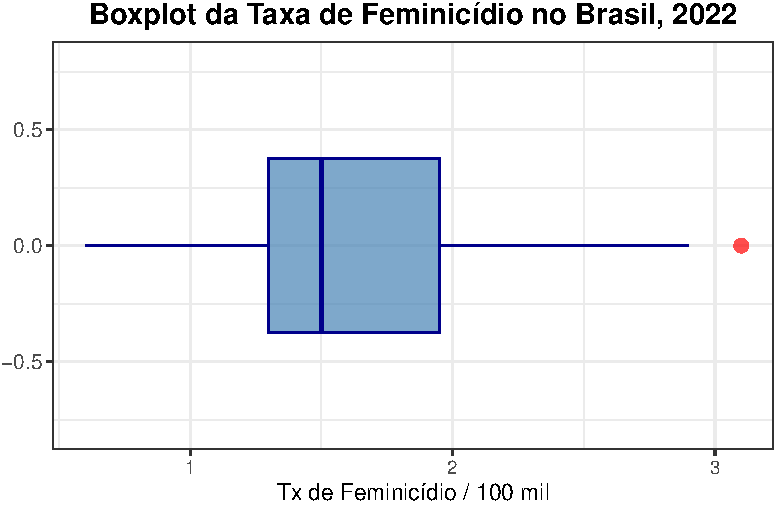
\includegraphics[keepaspectratio]{descritiva_v2_files/figure-pdf/unnamed-chunk-36-1.pdf}}

\begin{Shaded}
\begin{Highlighting}[]
\FunctionTok{ggplot}\NormalTok{(final\_fem\_22, }\FunctionTok{aes}\NormalTok{(}\AttributeTok{x =}\NormalTok{ regiao, }\AttributeTok{y =}\NormalTok{ feminic\_tx, }\AttributeTok{fill =}\NormalTok{ regiao)) }\SpecialCharTok{+}
  \FunctionTok{geom\_boxplot}\NormalTok{( }
    \AttributeTok{color =} \StringTok{"darkblue"}\NormalTok{, }\AttributeTok{alpha=}\FloatTok{0.7}\NormalTok{,                                     }\CommentTok{\# Boxplot linha azul, outlier vermelho e transparete }
    \AttributeTok{outlier.shape =} \DecValTok{16}\NormalTok{, }\AttributeTok{outlier.color =} \StringTok{"red"}\NormalTok{, }\AttributeTok{outlier.size =} \DecValTok{3}
\NormalTok{              ) }\SpecialCharTok{+} 
  \FunctionTok{labs}\NormalTok{(}
    \AttributeTok{title =} \StringTok{"Boxplot da Taxa de Feminicídio no Brasil, 2022"}\NormalTok{,         }\CommentTok{\# Título do gráfico, x e y e nome da legenda}
    \AttributeTok{x =} \StringTok{"Região"}\NormalTok{,                                                   }
    \AttributeTok{y =} \StringTok{"Tx de Feminicídio / 100 mil"}\NormalTok{,}
    \AttributeTok{fill =} \StringTok{"Região"}  \CommentTok{\# Rótulo do eixo y}
\NormalTok{      ) }\SpecialCharTok{+}
  \FunctionTok{coord\_flip}\NormalTok{() }\SpecialCharTok{+}                                                      \CommentTok{\# Inverte os eixos para horizontalidade}
  \FunctionTok{theme\_bw}\NormalTok{() }\SpecialCharTok{+} 
  \FunctionTok{theme}\NormalTok{(}
    \AttributeTok{plot.title =} \FunctionTok{element\_text}\NormalTok{(}\AttributeTok{hjust =} \FloatTok{0.5}\NormalTok{, }\AttributeTok{size =} \DecValTok{14}\NormalTok{, }\AttributeTok{face =} \StringTok{"bold"}\NormalTok{), }\CommentTok{\# Centraliza e estiliza o título}
    \AttributeTok{axis.text.y =} \FunctionTok{element\_text}\NormalTok{(}\AttributeTok{size =} \DecValTok{10}\NormalTok{),                           }\CommentTok{\# Ajusta o tamanho do texto no eixo y}
    \AttributeTok{axis.title.y =} \FunctionTok{element\_text}\NormalTok{(}\AttributeTok{size =} \DecValTok{12}\NormalTok{),                          }\CommentTok{\# Ajusta o tamanho do rótulo do eixo y}
    \AttributeTok{legend.position =} \FunctionTok{c}\NormalTok{(}\FloatTok{0.9}\NormalTok{,}\FloatTok{0.7}\NormalTok{)                                     }\CommentTok{\# Posição da Legenda quadrado de 1x1}
\NormalTok{  )}\SpecialCharTok{+}
\FunctionTok{scale\_fill\_brewer}\NormalTok{(}\AttributeTok{palette=}\StringTok{"Blues"}\NormalTok{)}
\end{Highlighting}
\end{Shaded}

\begin{verbatim}
Warning: A numeric `legend.position` argument in `theme()` was deprecated in ggplot2
3.5.0.
i Please use the `legend.position.inside` argument of `theme()` instead.
\end{verbatim}

\pandocbounded{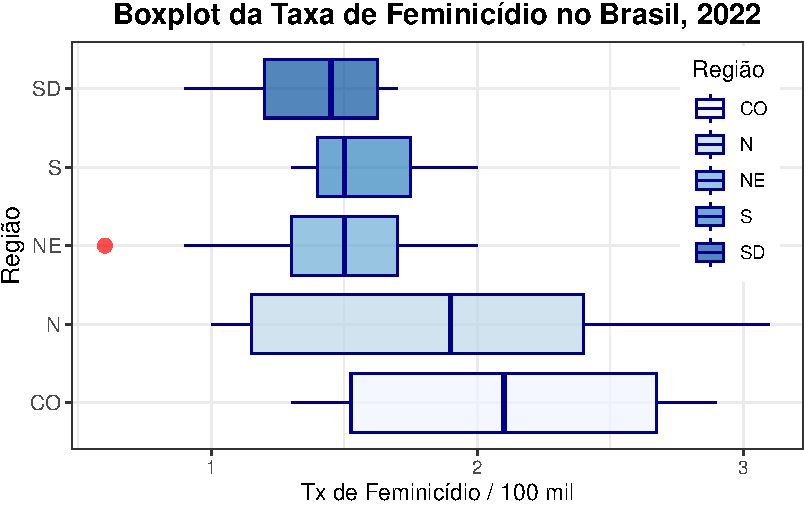
\includegraphics[keepaspectratio]{descritiva_v2_files/figure-pdf/unnamed-chunk-37-1.pdf}}

O Violin Plot é muito parecido com o BoxPlot mas com a densidade de
kernel rotacionada em cada um dos lados. Assim, indica a distribuição
dos dados em cada ponto e vem anotado a mediana na forma de um ponto ou
marca e um pequeno boxplot no centro do violin plot.

\begin{Shaded}
\begin{Highlighting}[]
\FunctionTok{library}\NormalTok{(dplyr)}

\NormalTok{final\_fem\_22 }\OtherTok{\textless{}{-}}\NormalTok{ final\_fem\_22 }\SpecialCharTok{\%\textgreater{}\%}
  \FunctionTok{mutate}\NormalTok{(}\AttributeTok{N\_NE\_CO =} \FunctionTok{case\_when}\NormalTok{(}
\NormalTok{    regiao }\SpecialCharTok{\%in\%} \FunctionTok{c}\NormalTok{(}\StringTok{"N"}\NormalTok{, }\StringTok{"NE"}\NormalTok{, }\StringTok{"CO"}\NormalTok{) }\SpecialCharTok{\textasciitilde{}} \DecValTok{1}\NormalTok{,  }\CommentTok{\# Região Norte, Nordeste e Centro{-}Oeste recebem 1}
    \ConstantTok{TRUE} \SpecialCharTok{\textasciitilde{}} \DecValTok{0}                             \CommentTok{\# Demais regiões recebem 0}
\NormalTok{  ))}

\CommentTok{\# Verificar a distribuição da variável N\_NE\_CO por região}
\FunctionTok{table}\NormalTok{(final\_fem\_22}\SpecialCharTok{$}\NormalTok{N\_NE\_CO, final\_fem\_22}\SpecialCharTok{$}\NormalTok{regiao)}
\end{Highlighting}
\end{Shaded}

\begin{verbatim}
   
    CO N NE S SD
  0  0 0  0 3  4
  1  4 7  9 0  0
\end{verbatim}

\begin{Shaded}
\begin{Highlighting}[]
\FunctionTok{ggplot}\NormalTok{(final\_fem\_22, }\FunctionTok{aes}\NormalTok{(}\AttributeTok{x =} \FunctionTok{factor}\NormalTok{(N\_NE\_CO, }\AttributeTok{labels =} \FunctionTok{c}\NormalTok{(}\StringTok{"Sul e Sudeste"}\NormalTok{, }\StringTok{"Norte, Nord. e C.Oeste"}\NormalTok{)),  }\CommentTok{\# Transformando em fatores}
                         \AttributeTok{y =}\NormalTok{ feminic\_tx, }\AttributeTok{fill =} \FunctionTok{factor}\NormalTok{(N\_NE\_CO))) }\SpecialCharTok{+}                                   \CommentTok{\# Taxa de Feminicídio por Fator}
  \FunctionTok{geom\_violin}\NormalTok{(}\AttributeTok{trim =} \ConstantTok{FALSE}\NormalTok{, }\AttributeTok{color =} \StringTok{"white"}\NormalTok{) }\SpecialCharTok{+}                                                        \CommentTok{\# Cria o gráfico de violino}
  \FunctionTok{scale\_fill\_manual}\NormalTok{(}\AttributeTok{values =} \FunctionTok{c}\NormalTok{(}\StringTok{"lightblue"}\NormalTok{, }\StringTok{"steelblue"}\NormalTok{)) }\SpecialCharTok{+}                                           \CommentTok{\# Cor das violas}
  \FunctionTok{stat\_summary}\NormalTok{(}\AttributeTok{fun=}\StringTok{"median"}\NormalTok{, }\AttributeTok{geom =} \StringTok{"point"}\NormalTok{, }\AttributeTok{shape=}\DecValTok{19}\NormalTok{, }\AttributeTok{size=}\DecValTok{3}\NormalTok{, }\AttributeTok{color=}\StringTok{"darkorange"}\NormalTok{  ) }\SpecialCharTok{+}                \CommentTok{\# Vamos colocar o ponto mediana}
  \FunctionTok{labs}\NormalTok{(}
    \AttributeTok{title =} \StringTok{"Violin Plots da taxa de feminicídio por região do Brasil"}\NormalTok{,}
    \AttributeTok{x =} \StringTok{"Região"}\NormalTok{,}
    \AttributeTok{y =} \StringTok{"Taxa de Feminicídio (por 100 mil)"}\NormalTok{,}
    \AttributeTok{fill =} \StringTok{"Região"}
\NormalTok{  ) }\SpecialCharTok{+}
  \FunctionTok{theme\_minimal}\NormalTok{() }\SpecialCharTok{+}
  \FunctionTok{theme}\NormalTok{(}
    \AttributeTok{plot.title =} \FunctionTok{element\_text}\NormalTok{(}\AttributeTok{hjust =} \FloatTok{0.5}\NormalTok{, }\AttributeTok{size =} \DecValTok{14}\NormalTok{, }\AttributeTok{face =} \StringTok{"bold"}\NormalTok{),              }\CommentTok{\# Centraliza o título}
    \AttributeTok{axis.text.x =} \FunctionTok{element\_text}\NormalTok{(}\AttributeTok{size =} \DecValTok{12}\NormalTok{),                                         }\CommentTok{\# Ajusta o tamanho dos rótulos no eixo X}
    \AttributeTok{axis.text.y =} \FunctionTok{element\_text}\NormalTok{(}\AttributeTok{size =} \DecValTok{10}\NormalTok{),                                         }\CommentTok{\# Ajusta o tamanho dos rótulos no eixo Y}
    \AttributeTok{legend.position =} \StringTok{"none"}\NormalTok{  )}
\end{Highlighting}
\end{Shaded}

\pandocbounded{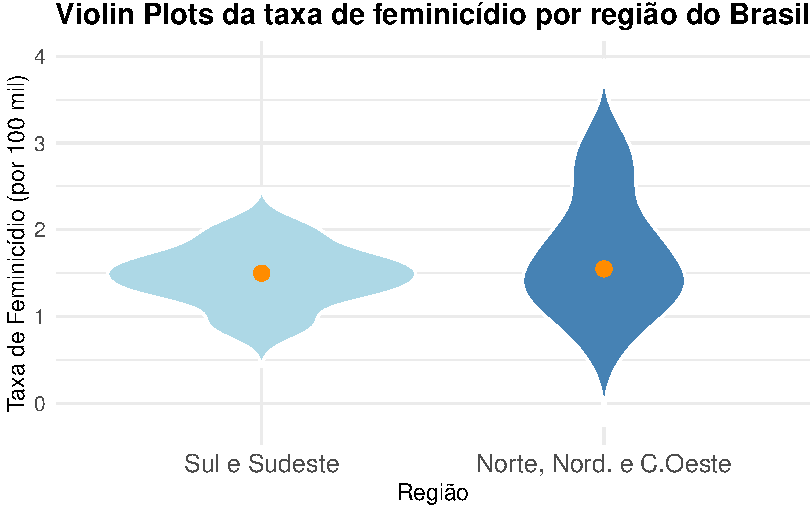
\includegraphics[keepaspectratio]{descritiva_v2_files/figure-pdf/unnamed-chunk-39-1.pdf}}

\textbf{Gráfico de Densidade}

Visualizar a distribuição empírica dos dados fornece uma grande
quantidade de informação. Um gráfico básico em análise descritiva é o
histograma, o qual fornece a distribuição de probabilidade empírica dos
dados em um formato de barras. A área do histograma é igual a 1 e altura
da sua barra da a densidade de observações em cada classe. ``\#c2986f'',
``Feminicídio'' = ``\#7185cc'')

\begin{Shaded}
\begin{Highlighting}[]
\FunctionTok{ggplot}\NormalTok{(final\_fem\_22, }\FunctionTok{aes}\NormalTok{(}\AttributeTok{x =}\NormalTok{ feminic\_tx)) }\SpecialCharTok{+}
  \FunctionTok{geom\_histogram}\NormalTok{(}\AttributeTok{bins =} \DecValTok{8}\NormalTok{, }\AttributeTok{fill =} \StringTok{"\#7185cc"}\NormalTok{, }\AttributeTok{color =} \StringTok{"white"}\NormalTok{, }\AttributeTok{alpha =} \FloatTok{0.7}\NormalTok{) }\SpecialCharTok{+}    \CommentTok{\# bins são os números de barras}
\CommentTok{\# Linha vertical com 70\% de transparência, que mostra a média da taxa de feminicídio}
  \FunctionTok{geom\_vline}\NormalTok{(}\FunctionTok{aes}\NormalTok{(}\AttributeTok{xintercept =} \FunctionTok{mean}\NormalTok{(feminic\_tx)), }\AttributeTok{color =} \StringTok{"\#c2986f"}\NormalTok{, }\AttributeTok{size =} \DecValTok{1}\NormalTok{, }\AttributeTok{alpha =} \FloatTok{0.7}\NormalTok{,}\AttributeTok{linetype =} \StringTok{"dashed"}\NormalTok{) }\SpecialCharTok{+}  
  \FunctionTok{labs}\NormalTok{(}
    \AttributeTok{x =} \StringTok{"Taxa de Feminicídio"}\NormalTok{,                                                  }\CommentTok{\# Título do eixo X, y e grafico}
    \AttributeTok{y =} \StringTok{"Frequência"}\NormalTok{,  }
    \AttributeTok{title =} \StringTok{"Histograma da Taxa de Feminicídio"}   
\NormalTok{  ) }\SpecialCharTok{+}
  \FunctionTok{theme\_minimal}\NormalTok{() }\SpecialCharTok{+} 
 \FunctionTok{theme}\NormalTok{(}
    \AttributeTok{plot.title =} \FunctionTok{element\_text}\NormalTok{(}\AttributeTok{hjust =} \FloatTok{0.5}\NormalTok{, }\AttributeTok{size =} \DecValTok{14}\NormalTok{, }\AttributeTok{face =} \StringTok{"bold"}\NormalTok{),              }\CommentTok{\# Centraliza o título}
    \AttributeTok{axis.text.x =} \FunctionTok{element\_text}\NormalTok{(}\AttributeTok{size =} \DecValTok{12}\NormalTok{),                                         }\CommentTok{\# Ajusta o tamanho dos rótulos no eixo X}
    \AttributeTok{axis.text.y =} \FunctionTok{element\_text}\NormalTok{(}\AttributeTok{size =} \DecValTok{10}\NormalTok{))}
\end{Highlighting}
\end{Shaded}

\begin{verbatim}
Warning: Using `size` aesthetic for lines was deprecated in ggplot2 3.4.0.
i Please use `linewidth` instead.
\end{verbatim}

\pandocbounded{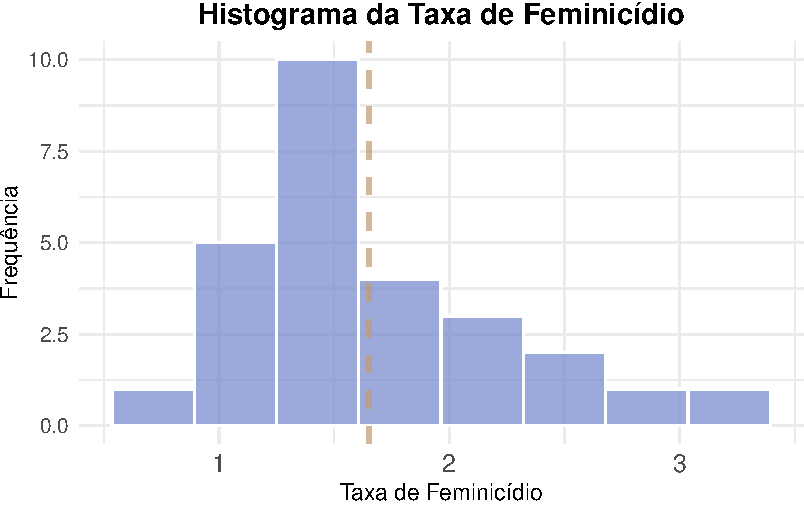
\includegraphics[keepaspectratio]{descritiva_v2_files/figure-pdf/unnamed-chunk-40-1.pdf}}

Uma outra maneira de visualizar os dados é utilizando uma distribuição
continua e não mais a discreta. Para isso, utiliza-se a densidade de
Kernel para visualização da distribuição de probabilidade da taxa de
feminicídio. Vejamos

\begin{Shaded}
\begin{Highlighting}[]
 \FunctionTok{ggplot}\NormalTok{(final\_fem\_22, }\FunctionTok{aes}\NormalTok{(}\AttributeTok{x =}\NormalTok{ feminic\_tx)) }\SpecialCharTok{+}
  \FunctionTok{geom\_density}\NormalTok{(}\AttributeTok{fill =} \StringTok{"\#7185cc"}\NormalTok{, }\AttributeTok{color =} \StringTok{"darkblue"}\NormalTok{, }\AttributeTok{alpha =} \FloatTok{0.6}\NormalTok{) }\SpecialCharTok{+}   \CommentTok{\# Curva de densidade e preenchimento}
   \FunctionTok{scale\_x\_continuous}\NormalTok{(}\AttributeTok{limits =} \FunctionTok{c}\NormalTok{(}\DecValTok{0}\NormalTok{, }\DecValTok{4}\NormalTok{)) }\SpecialCharTok{+}                               \CommentTok{\# Limita o eixo X entre 0 e 10  }
  \FunctionTok{labs}\NormalTok{(}
    \AttributeTok{x =} \StringTok{"Taxa de Feminicídio"}\NormalTok{,                                          }\CommentTok{\# Título do eixo X, Y e Gráfico}
    \AttributeTok{y =} \StringTok{"Densidade"}\NormalTok{,  }
    \AttributeTok{title =} \StringTok{"Densidade de Kernel para a Taxa de Feminicídio"}  
\NormalTok{  ) }\SpecialCharTok{+}
  \FunctionTok{theme\_minimal}\NormalTok{()  }\SpecialCharTok{+} 
 \FunctionTok{theme}\NormalTok{(}
    \AttributeTok{plot.title =} \FunctionTok{element\_text}\NormalTok{(}\AttributeTok{hjust =} \FloatTok{0.5}\NormalTok{, }\AttributeTok{size =} \DecValTok{14}\NormalTok{, }\AttributeTok{face =} \StringTok{"bold"}\NormalTok{),              }\CommentTok{\# Centraliza o título}
    \AttributeTok{axis.text.x =} \FunctionTok{element\_text}\NormalTok{(}\AttributeTok{size =} \DecValTok{12}\NormalTok{),                                         }\CommentTok{\# Ajusta o tamanho dos rótulos no eixo X}
    \AttributeTok{axis.text.y =} \FunctionTok{element\_text}\NormalTok{(}\AttributeTok{size =} \DecValTok{10}\NormalTok{))}
\end{Highlighting}
\end{Shaded}

\pandocbounded{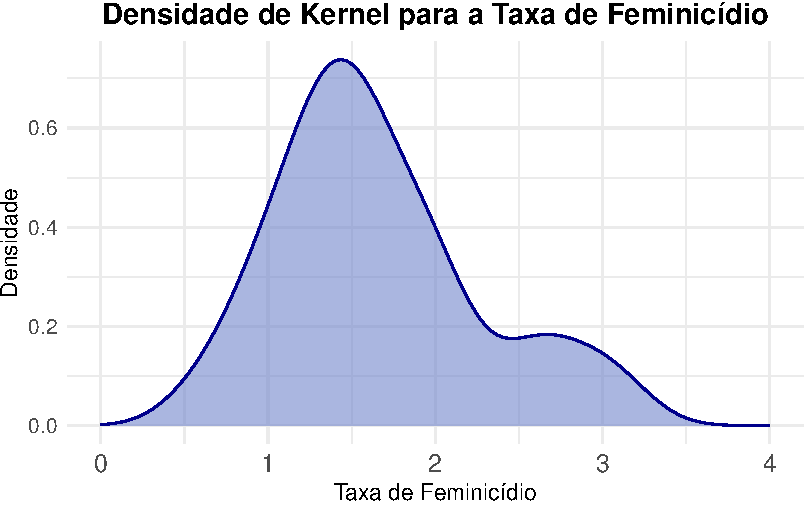
\includegraphics[keepaspectratio]{descritiva_v2_files/figure-pdf/unnamed-chunk-41-1.pdf}}

Podemos analisar mais de uma variável juntamente no gráfico acima. Vamos
ver a Taxa de Feminicídio e a Tentativa de Feminicídio

\begin{Shaded}
\begin{Highlighting}[]
 \FunctionTok{ggplot}\NormalTok{(final\_fem\_22) }\SpecialCharTok{+}
  \FunctionTok{geom\_density}\NormalTok{(}\FunctionTok{aes}\NormalTok{(}\AttributeTok{x =}\NormalTok{ feminic\_tx), }\AttributeTok{fill =} \StringTok{"\#7185cc"}\NormalTok{, }\AttributeTok{color =} \StringTok{"\#7185cc"}\NormalTok{, }\AttributeTok{alpha =} \FloatTok{0.6}\NormalTok{) }\SpecialCharTok{+}     \CommentTok{\# Curva de densidade e preenchimento}
  \FunctionTok{geom\_density}\NormalTok{(}\FunctionTok{aes}\NormalTok{(}\AttributeTok{x =}\NormalTok{ t\_feminic\_tx), }\AttributeTok{fill =} \StringTok{"\#c2986f"}\NormalTok{, }\AttributeTok{color =} \StringTok{"\#c2986f"}\NormalTok{, }\AttributeTok{alpha =} \FloatTok{0.6}\NormalTok{) }\SpecialCharTok{+}   \CommentTok{\# Curva de densidade e preenchimento}
  \FunctionTok{scale\_x\_continuous}\NormalTok{(}\AttributeTok{limits =} \FunctionTok{c}\NormalTok{(}\DecValTok{0}\NormalTok{, }\DecValTok{15}\NormalTok{)) }\SpecialCharTok{+}                                                   \CommentTok{\# Limita o eixo X entre 0 e 10  }
  \FunctionTok{labs}\NormalTok{(}
    \AttributeTok{x =} \StringTok{"Taxa de Feminicídio"}\NormalTok{,                                                             }\CommentTok{\# Título do eixo X, Y e Gráfico}
    \AttributeTok{y =} \StringTok{"Densidade"}\NormalTok{,  }
    \AttributeTok{title =} \StringTok{"Densidade de Kernel para a Taxa de Feminicídio"}\NormalTok{,}
    \AttributeTok{fill =} \StringTok{"Tipo"} 
\NormalTok{  ) }\SpecialCharTok{+}
  \FunctionTok{theme\_minimal}\NormalTok{()  }\SpecialCharTok{+}
 \FunctionTok{theme}\NormalTok{(}
    \AttributeTok{plot.title =} \FunctionTok{element\_text}\NormalTok{(}\AttributeTok{hjust =} \FloatTok{0.5}\NormalTok{, }\AttributeTok{size =} \DecValTok{14}\NormalTok{, }\AttributeTok{face =} \StringTok{"bold"}\NormalTok{),              }\CommentTok{\# Centraliza o título}
    \AttributeTok{axis.text.x =} \FunctionTok{element\_text}\NormalTok{(}\AttributeTok{size =} \DecValTok{12}\NormalTok{),                                         }\CommentTok{\# Ajusta o tamanho dos rótulos no eixo X}
    \AttributeTok{axis.text.y =} \FunctionTok{element\_text}\NormalTok{(}\AttributeTok{size =} \DecValTok{10}\NormalTok{)}
\NormalTok{    )}
\end{Highlighting}
\end{Shaded}

\pandocbounded{\includegraphics[keepaspectratio]{descritiva_v2_files/figure-pdf/unnamed-chunk-42-1.pdf}}

Outra forma útil de visualizar os dados a é distribuição por classe, por
exemplo distribuição de salários entre homens e mulheres, distribuição
do tempo do processo por vara, distribuição da taxa de feminicídio por
região. Vamos utilizar a densidade de Kernel para analisar a
distribuição dos valores da taxa de feminicídio por região. Para isso
precisa instalar o pacote \texttt{sm}.

\begin{Shaded}
\begin{Highlighting}[]
\FunctionTok{ggplot}\NormalTok{(final\_fem\_22, }\FunctionTok{aes}\NormalTok{(}\AttributeTok{x =}\NormalTok{ feminic\_tx, }\AttributeTok{fill =} \FunctionTok{factor}\NormalTok{(N\_NE\_CO))) }\SpecialCharTok{+} \CommentTok{\# Curvas de densidade para as duas regiões}
  \FunctionTok{geom\_density}\NormalTok{(}\AttributeTok{alpha =} \FloatTok{0.6}\NormalTok{, }\AttributeTok{color =} \StringTok{"white"}\NormalTok{) }\SpecialCharTok{+}
  \FunctionTok{scale\_fill\_manual}\NormalTok{(}\AttributeTok{values =} \FunctionTok{c}\NormalTok{(}\StringTok{"1"} \OtherTok{=} \StringTok{"\#7185cc"}\NormalTok{, }\StringTok{"0"} \OtherTok{=} \StringTok{"\#c2986f"}\NormalTok{), }
                    \AttributeTok{labels =} \FunctionTok{c}\NormalTok{(}\StringTok{"Norte, Nordeste, Centro{-}Oeste"}\NormalTok{, }\StringTok{"Sul e Sudeste"}\NormalTok{)) }\SpecialCharTok{+}
  \FunctionTok{scale\_x\_continuous}\NormalTok{(}\AttributeTok{limits =} \FunctionTok{c}\NormalTok{(}\DecValTok{0}\NormalTok{, }\DecValTok{5}\NormalTok{)) }\SpecialCharTok{+}
  \CommentTok{\# Adicionar rótulos e título}
  \FunctionTok{labs}\NormalTok{(}
    \AttributeTok{x =} \StringTok{"Taxa de Feminicídio"}\NormalTok{, }
    \AttributeTok{y =} \StringTok{"Densidade"}\NormalTok{,  }
    \AttributeTok{title =} \StringTok{"Comparação da Taxa de Feminicídio entre Regiões"}\NormalTok{, }
    \AttributeTok{fill =} \StringTok{"Região"}
\NormalTok{  ) }\SpecialCharTok{+}
  
  \CommentTok{\# Ajustar o tema e a aparência do gráfico}
  \FunctionTok{theme\_minimal}\NormalTok{() }\SpecialCharTok{+}
  \FunctionTok{theme}\NormalTok{(}
    \AttributeTok{plot.title =} \FunctionTok{element\_text}\NormalTok{(}\AttributeTok{hjust =} \FloatTok{0.5}\NormalTok{, }\AttributeTok{size =} \DecValTok{14}\NormalTok{, }\AttributeTok{face =} \StringTok{"bold"}\NormalTok{),}
    \AttributeTok{axis.text.x =} \FunctionTok{element\_text}\NormalTok{(}\AttributeTok{size =} \DecValTok{12}\NormalTok{),}
    \AttributeTok{axis.text.y =} \FunctionTok{element\_text}\NormalTok{(}\AttributeTok{size =} \DecValTok{10}\NormalTok{),}
    \AttributeTok{legend.position =} \StringTok{"top"}\NormalTok{,  }\CommentTok{\# Posição da legenda}
    \AttributeTok{legend.title =} \FunctionTok{element\_text}\NormalTok{(}\AttributeTok{size =} \DecValTok{10}\NormalTok{),}
    \AttributeTok{legend.text =} \FunctionTok{element\_text}\NormalTok{(}\AttributeTok{size =} \DecValTok{8}\NormalTok{)}
\NormalTok{  )}
\end{Highlighting}
\end{Shaded}

\pandocbounded{\includegraphics[keepaspectratio]{descritiva_v2_files/figure-pdf/unnamed-chunk-43-1.pdf}}

\begin{tcolorbox}[enhanced jigsaw, leftrule=.75mm, coltitle=black, colframe=quarto-callout-tip-color-frame, toprule=.15mm, opacitybacktitle=0.6, bottomtitle=1mm, bottomrule=.15mm, titlerule=0mm, toptitle=1mm, title=\textcolor{quarto-callout-tip-color}{\faLightbulb}\hspace{0.5em}{Exercício}, arc=.35mm, breakable, opacityback=0, colbacktitle=quarto-callout-tip-color!10!white, colback=white, left=2mm, rightrule=.15mm]

\textbf{PERGUNTA}: Gostaria de ter uma distribuição das Tentativa de
Feminicídio por Estado mostrando os quartis, mediana e média.

Dica: Utlizar a densidade e o boxplot?

\end{tcolorbox}

\begin{tcolorbox}[enhanced jigsaw, bottomrule=.15mm, leftrule=.75mm, arc=.35mm, colframe=quarto-callout-warning-color-frame, breakable, opacityback=0, toprule=.15mm, colback=white, left=2mm, rightrule=.15mm]
\begin{minipage}[t]{5.5mm}
\textcolor{quarto-callout-warning-color}{\faExclamationTriangle}
\end{minipage}%
\begin{minipage}[t]{\textwidth - 5.5mm}

\vspace{-3mm}\textbf{Veja a Resposta}\vspace{3mm}

\textbf{RESPOSTA}: Aqui segue uma sugestão de plotar a densidade
juntamente com o boxplot, possibilitando em um mesmo gráfico uma maior
quantidade de observação. Veja abaixo:

\begin{Shaded}
\begin{Highlighting}[]
\FunctionTok{library}\NormalTok{(ggplot2)}
\FunctionTok{library}\NormalTok{(gridExtra)}

\CommentTok{\# Criar o histograma com ggplot2}
\NormalTok{dens\_t\_f }\OtherTok{\textless{}{-}} \FunctionTok{ggplot}\NormalTok{(final\_fem\_22, }\FunctionTok{aes}\NormalTok{(}\AttributeTok{x =}\NormalTok{ t\_feminic\_tx)) }\SpecialCharTok{+}
  \FunctionTok{geom\_density}\NormalTok{(}\AttributeTok{fill =} \StringTok{"\#7185cc"}\NormalTok{, }\AttributeTok{color =} \StringTok{"darkblue"}\NormalTok{, }\AttributeTok{alpha =} \FloatTok{0.6}\NormalTok{) }\SpecialCharTok{+}
  \FunctionTok{geom\_vline}\NormalTok{(}\FunctionTok{aes}\NormalTok{(}\AttributeTok{xintercept =} \FunctionTok{mean}\NormalTok{(t\_feminic\_tx, }\AttributeTok{na.rm=}\ConstantTok{TRUE}\NormalTok{)), }\AttributeTok{color =} \StringTok{"\#c2986f"}\NormalTok{, }\AttributeTok{size =} \DecValTok{1}\NormalTok{, }\AttributeTok{alpha =} \FloatTok{0.7}\NormalTok{,}\AttributeTok{linetype =} \StringTok{"dashed"}\NormalTok{) }\SpecialCharTok{+}  
  \FunctionTok{scale\_x\_continuous}\NormalTok{(}\AttributeTok{limits =} \FunctionTok{c}\NormalTok{(}\DecValTok{0}\NormalTok{, }\DecValTok{15}\NormalTok{)) }\SpecialCharTok{+}
  \FunctionTok{labs}\NormalTok{(}\AttributeTok{x =} \StringTok{"Taxa de Feminicídio"}\NormalTok{, }\AttributeTok{y =} \StringTok{"Frequência"}\NormalTok{) }\SpecialCharTok{+}
  \FunctionTok{theme\_minimal}\NormalTok{()  }\SpecialCharTok{+}
  \FunctionTok{theme}\NormalTok{(}
    \AttributeTok{panel.background =} \FunctionTok{element\_blank}\NormalTok{(),  }\CommentTok{\# Remove o fundo do gráfico}
    \AttributeTok{plot.background =} \FunctionTok{element\_blank}\NormalTok{(),   }\CommentTok{\# Remove o fundo do gráfico}
    \AttributeTok{axis.line =} \FunctionTok{element\_blank}\NormalTok{(),         }\CommentTok{\# Remove as linhas dos eixos X e Y}
    \AttributeTok{axis.ticks =} \FunctionTok{element\_blank}\NormalTok{()        }\CommentTok{\# Remove os ticks dos eixos X e Y}
\NormalTok{  )}


\CommentTok{\# Criar o boxplot com ggplot2}
\NormalTok{bp\_t\_f }\OtherTok{\textless{}{-}} \FunctionTok{ggplot}\NormalTok{(final\_fem\_22, }\FunctionTok{aes}\NormalTok{(}\AttributeTok{x =}\NormalTok{ feminic\_tx)) }\SpecialCharTok{+}
  \FunctionTok{geom\_boxplot}\NormalTok{(}\AttributeTok{fill =} \StringTok{"\#c2986f"}\NormalTok{, }\AttributeTok{color =} \StringTok{"darkblue"}\NormalTok{, }\AttributeTok{outlier.shape =} \DecValTok{16}\NormalTok{, }\AttributeTok{outlier.size =} \DecValTok{3}\NormalTok{) }\SpecialCharTok{+}
  \FunctionTok{labs}\NormalTok{(}\AttributeTok{x =} \ConstantTok{NULL}\NormalTok{, }\AttributeTok{y =} \ConstantTok{NULL}\NormalTok{) }\SpecialCharTok{+}
  \FunctionTok{theme}\NormalTok{(}
    \AttributeTok{panel.background =} \FunctionTok{element\_blank}\NormalTok{(),  }\CommentTok{\# Remove o fundo do painel}
    \AttributeTok{plot.background =} \FunctionTok{element\_blank}\NormalTok{(),   }\CommentTok{\# Remove o fundo do gráfico}
    \AttributeTok{axis.line =} \FunctionTok{element\_blank}\NormalTok{(),         }\CommentTok{\# Remove as linhas dos eixos X e Y}
    \AttributeTok{axis.ticks =} \FunctionTok{element\_blank}\NormalTok{(),        }\CommentTok{\# Remove os ticks dos eixos X e Y}
    \AttributeTok{axis.text =} \FunctionTok{element\_blank}\NormalTok{() )         }\CommentTok{\# Remove os textos dos eixos X e Y}
  

\CommentTok{\# Organizar os gráficos usando grid.arrange}
\FunctionTok{grid.arrange}\NormalTok{( bp\_t\_f, dens\_t\_f,}
             \AttributeTok{ncol =} \DecValTok{1}\NormalTok{, }\AttributeTok{heights =} \FunctionTok{c}\NormalTok{(}\DecValTok{1}\NormalTok{, }\DecValTok{4}\NormalTok{))}
\end{Highlighting}
\end{Shaded}

\pandocbounded{\includegraphics[keepaspectratio]{descritiva_v2_files/figure-pdf/unnamed-chunk-44-1.pdf}}

\end{minipage}%
\end{tcolorbox}

\section{Medidas de Associação}\label{medidas-de-associauxe7uxe3o}

\textbf{COVARIÂNCIA AMOSTRAL}

Covariância entre duas variáveis: A covariância entre duas variáveis X e
Y é uma medida estatística que descreve como essas variáveis variam
juntas. Em outras palavras, a covariância indica a tendência de X e Y de
se moverem na mesma direção (covariância positiva) ou em direções
opostas (covariância negativa).

\[\text{Cov}(X, Y) = \frac{1}{n-1} \sum_{i=1}^{n} (X_i - \bar{X})(Y_i - \bar{Y})\]

\begin{Shaded}
\begin{Highlighting}[]
 \FunctionTok{cov}\NormalTok{(final\_fem\_22}\SpecialCharTok{$}\NormalTok{feminic\_tx, final\_fem\_22}\SpecialCharTok{$}\NormalTok{homic\_tx)}
\end{Highlighting}
\end{Shaded}

\begin{verbatim}
[1] 0.4648575
\end{verbatim}

\textbf{CORRELAÇÃO}

O coeficiente de correlação entre duas variáveis X e Y é uma medida
estatística que descreve a força e a direção da relação linear entre
essas variáveis. O coeficiente de correlação é frequentemente
representado pelo coeficiente de correlação de Pearson, \(r_{XY}\).

\[r_{XY} = \frac{\text{Cov}(X, Y)}{s_X s_Y}\] O coeficiente de
correlação de Pearson é uma medida amplamente utilizada para avaliar a
relação linear entre variáveis, pois fornece uma interpretação
padronizada da força e direção da relação, independentemente das
unidades das variáveis.

\begin{Shaded}
\begin{Highlighting}[]
 \FunctionTok{cor}\NormalTok{(final\_fem\_22}\SpecialCharTok{$}\NormalTok{feminic\_tx, final\_fem\_22}\SpecialCharTok{$}\NormalTok{homic\_tx)}
\end{Highlighting}
\end{Shaded}

\begin{verbatim}
[1] 0.3589068
\end{verbatim}

\subsubsection{Visualizando a
Associação}\label{visualizando-a-associauxe7uxe3o}

\textbf{Scatter Plot}

O Scatter Plot é conhecido como o gráfico de dispersão. Ele relaciona
duas ou três variáveis, ou seja, plota \(X\) contra \(Y\). Muito
utilizado para ver o comportamento conjunto de duas séries.

Como já visto que renda pc e a taxa de feminicídio não mostram um
comportamento conjunto:

\begin{Shaded}
\begin{Highlighting}[]
\FunctionTok{ggplot}\NormalTok{(}\AttributeTok{data =}\NormalTok{ final\_fem\_22, }\FunctionTok{aes}\NormalTok{(}\AttributeTok{x =}\NormalTok{ rendapc, }\AttributeTok{y =}\NormalTok{ feminic\_tx))}\SpecialCharTok{+}
  \FunctionTok{geom\_point}\NormalTok{(}\AttributeTok{color=}\StringTok{"\#6e94bd"}\NormalTok{, }\AttributeTok{size=}\DecValTok{3}\NormalTok{, }\AttributeTok{alpha=}\FloatTok{0.7}\NormalTok{,  }\AttributeTok{shape=}\DecValTok{17}\NormalTok{) }\SpecialCharTok{+}
  \FunctionTok{scale\_y\_continuous}\NormalTok{(}\AttributeTok{limits =} \FunctionTok{c}\NormalTok{(}\DecValTok{0}\NormalTok{, }\DecValTok{5}\NormalTok{)) }\SpecialCharTok{+}
  \FunctionTok{geom\_smooth}\NormalTok{(}\AttributeTok{method =} \StringTok{"lm"}\NormalTok{, }\AttributeTok{se=}\ConstantTok{TRUE}\NormalTok{ , }\AttributeTok{color=}\StringTok{"orange"}\NormalTok{)}\SpecialCharTok{+}
  \FunctionTok{labs}\NormalTok{(}\AttributeTok{title=}\StringTok{"Renda pc e taxa de Feminicídios por Estado"}\NormalTok{, }\AttributeTok{x=}\StringTok{"Renda pc"}\NormalTok{, }\AttributeTok{y=}\StringTok{"Tx 100 mil"}\NormalTok{)}\SpecialCharTok{+}
  \FunctionTok{theme\_bw}\NormalTok{()}
\end{Highlighting}
\end{Shaded}

\pandocbounded{\includegraphics[keepaspectratio]{descritiva_v2_files/figure-pdf/unnamed-chunk-47-1.pdf}}

Ao observar o homicídio absoluto e o feminicídio absoluto, estados com
maiores números de homicídio tendem a ter maior número de feminicídios.

\begin{Shaded}
\begin{Highlighting}[]
\CommentTok{\# Primeiro vou fzer a correlação}
\NormalTok{correl1}\OtherTok{\textless{}{-}}\FunctionTok{cor}\NormalTok{(final\_fem\_22}\SpecialCharTok{$}\NormalTok{part\_feminic, final\_fem\_22}\SpecialCharTok{$}\NormalTok{homic\_tx)}

\CommentTok{\#Depois montamos o Gráfico e anotamos a correlação no gráfico}
\FunctionTok{ggplot}\NormalTok{(}\AttributeTok{data =}\NormalTok{ final\_fem\_22, }\FunctionTok{aes}\NormalTok{(}\AttributeTok{x =}\NormalTok{ part\_feminic, }\AttributeTok{y =}\NormalTok{ homic\_tx))}\SpecialCharTok{+}
  \FunctionTok{geom\_point}\NormalTok{(}\AttributeTok{color=}\StringTok{"\#6e94bd"}\NormalTok{, }\AttributeTok{size=}\DecValTok{3}\NormalTok{, }\AttributeTok{alpha=}\FloatTok{0.7}\NormalTok{,  }\AttributeTok{shape=}\DecValTok{17}\NormalTok{) }\SpecialCharTok{+}
  \FunctionTok{geom\_smooth}\NormalTok{(}\AttributeTok{method =} \StringTok{"lm"}\NormalTok{, }\AttributeTok{se=}\ConstantTok{TRUE}\NormalTok{ , }\AttributeTok{color=}\StringTok{"orange"}\NormalTok{)}\SpecialCharTok{+}
  \FunctionTok{labs}\NormalTok{(}\AttributeTok{title=}\StringTok{"Taxa de Homicídio por 100 mil mulheres e a Participação do Feminicídio"}\NormalTok{,}
       \AttributeTok{x=}\StringTok{"Participação do Feminicídio"}\NormalTok{, }
       \AttributeTok{y=}\StringTok{"Taxa de Homicídio"}\NormalTok{)}\SpecialCharTok{+}
  \FunctionTok{annotate}\NormalTok{(}
    \StringTok{"text"}\NormalTok{, }
    \AttributeTok{x=}\DecValTok{40}\NormalTok{, }\AttributeTok{y=}\DecValTok{9}\NormalTok{,}
    \AttributeTok{label =} \FunctionTok{paste}\NormalTok{(}\StringTok{"Correlação: "}\NormalTok{, }\FunctionTok{round}\NormalTok{(correl1, }\DecValTok{2}\NormalTok{)), }
    \AttributeTok{color =} \StringTok{"\#6e94bd"}\NormalTok{, }\AttributeTok{size =} \DecValTok{4}\NormalTok{, }\AttributeTok{hjust =} \DecValTok{0}
\NormalTok{  ) }\SpecialCharTok{+}
  \FunctionTok{theme\_bw}\NormalTok{()}
\end{Highlighting}
\end{Shaded}

\pandocbounded{\includegraphics[keepaspectratio]{descritiva_v2_files/figure-pdf/unnamed-chunk-48-1.pdf}}

\textbf{Correlograma}

Correlograma é uma maneira de analisar todas as correlações de umaúnca
vez a partir de uma matriz.

\begin{Shaded}
\begin{Highlighting}[]
\FunctionTok{library}\NormalTok{(corrgram)}
\NormalTok{correl}\OtherTok{\textless{}{-}}\NormalTok{ final\_fem\_22[}\FunctionTok{c}\NormalTok{(}\DecValTok{5}\NormalTok{,}\DecValTok{7}\NormalTok{,}\DecValTok{8}\NormalTok{,}\DecValTok{9}\NormalTok{,}\DecValTok{13}\NormalTok{,}\DecValTok{15}\NormalTok{,}\DecValTok{16}\NormalTok{)]}
\FunctionTok{corrgram}\NormalTok{(correl, }\AttributeTok{order=}\ConstantTok{TRUE}\NormalTok{, }\AttributeTok{lower.panel=}\NormalTok{panel.shade, }\AttributeTok{upper.panel=}\NormalTok{panel.cor,  }\AttributeTok{main=}\StringTok{"Correlação entre as diversas variáveis"}\NormalTok{) }
\end{Highlighting}
\end{Shaded}

\pandocbounded{\includegraphics[keepaspectratio]{descritiva_v2_files/figure-pdf/unnamed-chunk-49-1.pdf}}

\begin{Shaded}
\begin{Highlighting}[]
\CommentTok{\#install.packages("ggcorrplot")}
\FunctionTok{library}\NormalTok{(ggcorrplot)}
\NormalTok{correl2}\OtherTok{\textless{}{-}} \FunctionTok{round}\NormalTok{(}\FunctionTok{cor}\NormalTok{(final\_fem\_22[}\FunctionTok{c}\NormalTok{(}\DecValTok{5}\SpecialCharTok{:}\DecValTok{9}\NormalTok{, }\DecValTok{12}\NormalTok{)]),}\DecValTok{2}\NormalTok{)}
\FunctionTok{ggcorrplot}\NormalTok{(correl2, }\AttributeTok{hc.order =} \ConstantTok{TRUE}\NormalTok{, }\AttributeTok{type =} \StringTok{"lower"}\NormalTok{,        }\CommentTok{\# Matriz de correlação, coloca de forma ordenada e inferior}
           \AttributeTok{lab =} \ConstantTok{TRUE}\NormalTok{, }\AttributeTok{lab\_size =} \DecValTok{3}\NormalTok{, }\AttributeTok{lab\_col =} \StringTok{"\#616161"}\NormalTok{,   }\CommentTok{\#  mostra os valores tamanho 4}
           \AttributeTok{outline.col =} \StringTok{"white"}\NormalTok{,}
           \AttributeTok{ggtheme =}\NormalTok{ ggplot2}\SpecialCharTok{::}\NormalTok{theme\_minimal,}
           \AttributeTok{colors =} \FunctionTok{c}\NormalTok{(}\StringTok{"\#6D9EC1"}\NormalTok{, }\StringTok{"white"}\NormalTok{, }\StringTok{"\#c2986f"}\NormalTok{))}\SpecialCharTok{+}     \CommentTok{\# cores utilizadas}
\CommentTok{\# Colocando nomes  }
  \FunctionTok{labs}\NormalTok{(}\AttributeTok{title =} \StringTok{"Correlação entre as Diversas Variáveis"}\NormalTok{)}\SpecialCharTok{+}   \CommentTok{\# Título}
\CommentTok{\#Trocando os nomes das variáveis}
  \FunctionTok{scale\_y\_discrete}\NormalTok{(}\AttributeTok{labels =} \FunctionTok{c}\NormalTok{(}\StringTok{"Feminic. Abs."}\NormalTok{, }\StringTok{"Part. Feminic."}\NormalTok{, }\StringTok{"Renda pc"}\NormalTok{,  }\CommentTok{\# Nomes no eixo X}
                              \StringTok{"Taxa Homic."}\NormalTok{, }\StringTok{"Homic. Abs."}\NormalTok{)) }\SpecialCharTok{+}  
  \FunctionTok{scale\_x\_discrete}\NormalTok{(}\AttributeTok{labels =} \FunctionTok{c}\NormalTok{(}\StringTok{"Part. Feminic."}\NormalTok{, }\StringTok{"Renda pc"}\NormalTok{, }
                              \StringTok{"Taxa Homic."}\NormalTok{, }\StringTok{"Homic. Abs."}\NormalTok{, }\StringTok{"Taxa Feminic."}\NormalTok{))  }\CommentTok{\# Nomes no eixo Y}
\end{Highlighting}
\end{Shaded}

\pandocbounded{\includegraphics[keepaspectratio]{descritiva_v2_files/figure-pdf/unnamed-chunk-50-1.pdf}}

Salvando nosso banco para a próxima seção

\begin{Shaded}
\begin{Highlighting}[]
\FunctionTok{save}\NormalTok{(final\_fem\_22, }\AttributeTok{file =} \StringTok{"final\_fem\_22.RData"}\NormalTok{)}
\end{Highlighting}
\end{Shaded}

\bookmarksetup{startatroot}

\chapter{Uma Introdução à
Estatística}\label{uma-introduuxe7uxe3o-uxe0-estatuxedstica}

Conceitos Inciciais

\hfill\break

\section{Porque Estudar
Estatística?}\label{porque-estudar-estatuxedstica}

Podemos dizer que a existência da estatística e de outras ciências está
conectada a existência de problemas. Não somente a ciência mas o nosso
trabalho está conectado a superação de problemas cotidianos. Tomar
decisão é o dia a dia do gestor.

Segundo Popper ``we study not disciplines, but problems. Often, problems
transcend the boundaries of a particular discipline''

A questão central é: Como solucionamos os problemas? Utilizamos a melhor
estratégia? A solução foi boa?

\includegraphics[width=6.54in,height=1.86in]{estatistica_files/figure-latex/mermaid-figure-1.png}

\subsection{Os dois sistemas
cognitivos}\label{os-dois-sistemas-cognitivos}

Os livros abaixo são boas referências sobre a tomada de decisão.

\begin{figure}

\begin{minipage}{0.30\linewidth}

\begin{figure}[H]

{\centering \includegraphics[width=0.5\linewidth,height=\textheight,keepaspectratio]{figuras/kahneman.jpg}

}

\subcaption{Kahneman: Rápido e Devagar- Duas Formas de Pensar}

\end{figure}%

\end{minipage}%
%
\begin{minipage}{0.40\linewidth}
~\end{minipage}%
%
\begin{minipage}{0.30\linewidth}

\begin{figure}[H]

{\centering \includegraphics[width=0.5\linewidth,height=\textheight,keepaspectratio]{figuras/bazerman.jpg}

}

\subcaption{Bazerman e Moore: Processo Decisório}

\end{figure}%

\end{minipage}%

\end{figure}%

Existem dois sistemas que utilizamos para tomar decisão. O chamado
\textbf{Sistema 1} e o chamado \textbf{Sistema 2}. Segue uma breve
descrição de cada um:

\textbf{Sistema 1}:

\begin{itemize}
\tightlist
\item
  Intuitivo, rápido, automático, sem esforço, implícito e emocional

  \begin{itemize}
  \tightlist
  \item
    Pressa,
  \item
    Falta de tempo,
  \item
    Problemas menos importante
  \item
    Mais Falhas/Erros
  \end{itemize}
\end{itemize}

\textbf{Sistema 2}

\begin{itemize}
\tightlist
\item
  Raciocíonio lento, consciente, esforçado, explícito, lógico

  \begin{itemize}
  \tightlist
  \item
    Requer tempo,
  \item
    Mais recursos
  \item
    Problemas mais importante
  \item
    Menos Falhas
  \end{itemize}
\end{itemize}

Para o Sistema 1 usamos a nossa intuição que chamamos de Heurística.
Vejamos um pouco mais sobre esse sistema.

\textbf{HEURÍSTICA}

São rotinas inconscientes ou atalhos que o nosso cérebro utiliza para
lidar com a complexidade.

\begin{itemize}
\tightlist
\item
  Modelo/Regras Intuitivas.
\item
  Próprio do Sistema 1.
\item
  Apesar de processo sofisticado, são passíveis de falhas. Intuição
  falha
\end{itemize}

\ul{\textbf{Um Exemplo}}

Veja a figura abaixo retirada do livro do Bazerman.Responda rápido.

\textbf{Qual delas tem o tampo mais quadrado?}

\begin{figure}[H]

{\centering \includegraphics[width=0.8\linewidth,height=\textheight,keepaspectratio]{figuras/mesa.jpg}

}

\caption{Bazerman: Exemplo das mesas}

\end{figure}%

Se você achou que é a segunda mesa, você está alinhado com a grande
maioria. Nesse caso você usou o seu sistema 1

Vamos repitir a pergunta:

\textbf{Qual delas tem o tampo mais quadrado?}

Agora use uma régua para medir as mesas. Usamos aqui o sistema 2. Mais
tempo e recursos são utlizados. Qual mesa agora você considera mais
quadrada? Mudou sua opinião?

Com a régua vemos que as mesas são iguais. Isso mostra que a nossa
intuição \textbf{FALHA}.

\textbf{Tipos de Heurísticas}

\begin{itemize}
\item
  \textbf{Heurística da disponibilidade}: Usamos o que está mais próximo
  na memória para calcular a probabilidade.
\item
  \textbf{Heurística da representatividade}: Buscamos aquilo que reforça
  o padrão.
\item
  \textbf{Heurística da hipótese positiva}: Assumimos que uma
  determinada hipótese é verdadeira e não olhamos o contrafactual.
\item
  \textbf{Heurística do afeto}: Decisão considera o emocional. Seu humor
  afetam as decisões.
\end{itemize}

Para contornar os problemas da intuição e seus viéses na tomada de
decisão o primeiro passo é compreender que eles existem e estarmos
alerta. E para problemas maiores o uso do sistema 2 torna-se relevante.

Uma das principais ferramentas do sistema 2 é a Estatística. Com os
avanços computacionais essa ciência tem se destacado como um dos
elementos centrais do \emph{data science}. Abaixo a figura resume as
diversas áreas de desenvolvimento da análise de dados, obviamente não
exaustiva:

\begin{figure}[H]

{\centering \includegraphics[width=0.8\linewidth,height=\textheight,keepaspectratio]{figuras/analisedados.jpg}

}

\caption{Fluxograma da Análise de Dados}

\end{figure}%

Nosso objetivo é explorar nessa seção a análise descritiva. Chamado hoje
no \emph{Business Intelligence}, que e uma das áreas do \emph{Data
Science}.

\section{Conceitos Básicos de
Estatística}\label{conceitos-buxe1sicos-de-estatuxedstica}

Novamente começamos com um problema e esse definirá a nossa análise.
Vejamos alguns problemas que poderiam nos interessar\ldots{}

\begin{tcolorbox}[enhanced jigsaw, leftrule=.75mm, coltitle=black, colframe=quarto-callout-note-color-frame, toprule=.15mm, opacitybacktitle=0.6, bottomtitle=1mm, bottomrule=.15mm, titlerule=0mm, toptitle=1mm, title=\textcolor{quarto-callout-note-color}{\faInfo}\hspace{0.5em}{Problema 1}, arc=.35mm, breakable, opacityback=0, colbacktitle=quarto-callout-note-color!10!white, colback=white, left=2mm, rightrule=.15mm]

O prefeito de Ribeirão Preto vai lançar uma política que fornece
vouchers de alimentação para mulheres que estão em situação de pobreza.

\textbf{Problema}: \ul{Qual o valor que devo reservar ao programa?
Quantas mulheres serão atendidas?}

\end{tcolorbox}

\begin{tcolorbox}[enhanced jigsaw, leftrule=.75mm, coltitle=black, colframe=quarto-callout-note-color-frame, toprule=.15mm, opacitybacktitle=0.6, bottomtitle=1mm, bottomrule=.15mm, titlerule=0mm, toptitle=1mm, title=\textcolor{quarto-callout-note-color}{\faInfo}\hspace{0.5em}{Problema 2}, arc=.35mm, breakable, opacityback=0, colbacktitle=quarto-callout-note-color!10!white, colback=white, left=2mm, rightrule=.15mm]

O TJSP vai lançar um programa para reduzir o tempo médio em processos de
feminicídio.

\textbf{Problema}: \ul{Qual o tempo médio de um processo de
feminicídio?}

\end{tcolorbox}

\begin{tcolorbox}[enhanced jigsaw, leftrule=.75mm, coltitle=black, colframe=quarto-callout-note-color-frame, toprule=.15mm, opacitybacktitle=0.6, bottomtitle=1mm, bottomrule=.15mm, titlerule=0mm, toptitle=1mm, title=\textcolor{quarto-callout-note-color}{\faInfo}\hspace{0.5em}{Problema 3}, arc=.35mm, breakable, opacityback=0, colbacktitle=quarto-callout-note-color!10!white, colback=white, left=2mm, rightrule=.15mm]

O O governo federal vai lançar um programa para capacitar mulheres que
estão fora do mercado de trabalho.

\textbf{Problema}: \ul{Quantas mulheres serão alvos dessa política?}

\end{tcolorbox}

\subsection{A Variável Aleatória}\label{a-variuxe1vel-aleatuxf3ria}

O problema nos define a população que estou interessado. Vamos seguir, a
princípio, com o nosso probelma 1 para definirmos alguns conceitos
importantes.

\textbf{No problema 1}: me interessa compreender a renda das mulheres
que moram em Ribeirão Preto em dado ano. Para ficar simples vamos
abreviar o que nos interessa

\[X=\text{Renda das mulheres que moram em Ribeirão Preto em determinado ano}\]
Agora posso utilizar o X no lugar do nome. Olhando para a população e
pensando que cada nível de renda pode ser representada por uma cor,
teremos a seguinte imagem pouco de como a renda se distribui nessa
população:

\begin{figure}[H]

{\centering \includegraphics[width=0.5\linewidth,height=\textheight,keepaspectratio]{figuras/lego.jpg}

}

\caption{Renda pc das mulheres de Ribeirão Preto.}

\end{figure}%

A questão é: quais cores existem e quantas peças de cada cor temos? Para
isso usamos um experimento

\textbf{EXPERIMENTO ALEATÓRIO}

O experimento em ciências sociais aplicadas em geral está associada a
observação sistemática de pessoas, cidades, empresas ou processos. A
ideia é:

\begin{itemize}
\tightlist
\item
  Sortear pessoas e observar a sua caracteristica de forma indefinida e
  sempre na mesma condição.\\
\item
  Não consigo dizer o que vai sair no próximo sorteio, apenas consigo
  descrever os resultados possíveis
\item
  Se repetir o experimento um número grande de vezes uma regularidade
  aparece.
\end{itemize}

Se eu conseguir sortear de forma indefinida e na mesma condição as
mulheres que moram em Ribeirão Preto e perguntar sobre a sua renda. Eu
consigo reorganizar a figura acima da seguinte forma:

\begin{figure}[H]

{\centering \includegraphics[width=0.5\linewidth,height=\textheight,keepaspectratio]{figuras/lego_org.jpg}

}

\caption{Renda pc das mulheres de Ribeirão Preto.}

\end{figure}%

\textbf{ESPAÇO AMOSTRAL}

Agora conseguimos organizar os nossos resultados em um lugar chamado
espaço amostral. Nele teremos todas as cores (azul, branca,
amarela\ldots) que podem acontecer e o número de peças de cada cor (a
chance). Em outras palavras teremos todos os possíveis valores de \(X\)
e suas probabilidades.

\textbf{VARIÁVEL ALEATÓRIA}

Quanto representamos esse espaço amostral em formato de números é o que
chamamos de Variável Aleatória (V.A.). A V.A. é a combinação de tudo que
pode acontecer, ou seja, todas as rendas que existem associadas a
probabilidade de cada uma das rendas acontecerem.

Existem dois tipos principais de variáveis aleatórias: discretas e
contínuas.

\textbf{VARIÁVEIS ALEATÓRIAS DISCRETAS}

É um tipo de variável que conseguimos colocar em lista, seja finita ou
infinita \(x_1; x_2;...; x_n;...\) e associa-se a cada um dessses
valores uma probabilidade \(p(x_1); p(x_2);...; p(x_n);...\)

Podemos pensar aqui se a pessoa é casada, solteira, divorciada, viúva ou
outra condição. Se no processo classificamos como homicídio ou
feminicídio, se mora na área urbana ou rural\ldots{}

Na figura abaixo iremos coletar de 20 processos de homicídio e
gostariamos de saber quando é classificado como feminicídio e quanto é
classificado como homicídio (p=0,3).

\begin{Shaded}
\begin{Highlighting}[]
\NormalTok{feminicidio }\OtherTok{\textless{}{-}} \DecValTok{0}\SpecialCharTok{:}\DecValTok{20}

\FunctionTok{plot}\NormalTok{(feminicidio,}\FunctionTok{dbinom}\NormalTok{(feminicidio,}\AttributeTok{size=}\DecValTok{20}\NormalTok{,}\AttributeTok{prob=}\NormalTok{.}\DecValTok{3}\NormalTok{),}
     \AttributeTok{type=}\StringTok{\textquotesingle{}h\textquotesingle{}}\NormalTok{,}
     \AttributeTok{main=}\StringTok{\textquotesingle{}Distribuição Binomial (n=20, p=0.3)\textquotesingle{}}\NormalTok{,}
     \AttributeTok{ylab=}\StringTok{\textquotesingle{}Probabilidade\textquotesingle{}}\NormalTok{,}
     \AttributeTok{xlab =}\StringTok{\textquotesingle{}Feminicídio\textquotesingle{}}\NormalTok{,}
     \AttributeTok{lwd=}\DecValTok{3}\NormalTok{)}
\end{Highlighting}
\end{Shaded}

\begin{figure}[H]

{\centering \pandocbounded{\includegraphics[keepaspectratio]{estatistica_files/figure-pdf/unnamed-chunk-2-1.pdf}}

}

\caption{Distribuição Normal}

\end{figure}%

\textbf{VARIÁVEIS ALEATÓRIAS CONTÍNUAS}

Por outro lado, uma variável aleatória contínua pode assumir infinito
valores dentro de um intervalo específico. Agora temos infinitas
possibilidades de resultados para \(X\) e agora associamos uma função
\(f(x)\) que irá descrever o comportamento da probabilidade.

Por exemplo, a altura de uma pessoa, a sua renda, a sua idade, o tempo
que demora um processo.

Abaixo temos uma representação de uma distriuição continua da renda das
mulheres em Ribeirão Preto, chamada distribuição normal:

\begin{Shaded}
\begin{Highlighting}[]
\FunctionTok{rm}\NormalTok{(}\AttributeTok{list =} \FunctionTok{ls}\NormalTok{(}\AttributeTok{all.names =} \ConstantTok{TRUE}\NormalTok{)) }\CommentTok{\#will clear all objects includes hidden objects.}
\NormalTok{x}\OtherTok{\textless{}{-}}\FunctionTok{seq}\NormalTok{(}\DecValTok{700}\NormalTok{,}\DecValTok{1300}\NormalTok{,}\DecValTok{1}\NormalTok{)}
\NormalTok{fdnorm}\OtherTok{\textless{}{-}}\FunctionTok{dnorm}\NormalTok{(}\AttributeTok{x =}\NormalTok{ x, }\AttributeTok{mean =} \DecValTok{1000}\NormalTok{, }\AttributeTok{sd=}\DecValTok{100}\NormalTok{)  }
\NormalTok{fdanorm}\OtherTok{\textless{}{-}}\FunctionTok{pnorm}\NormalTok{(}\AttributeTok{q =}\NormalTok{ x, }\AttributeTok{mean =} \DecValTok{1000}\NormalTok{, }\AttributeTok{sd=}\DecValTok{100}\NormalTok{)}
\FunctionTok{curve}\NormalTok{(}\FunctionTok{dnorm}\NormalTok{(x,}\DecValTok{1000}\NormalTok{,}\DecValTok{100}\NormalTok{),}\AttributeTok{xlim=}\FunctionTok{c}\NormalTok{(}\DecValTok{700}\NormalTok{,}\DecValTok{1300}\NormalTok{),}\AttributeTok{main=}\StringTok{\textquotesingle{}\textquotesingle{}}\NormalTok{,}\AttributeTok{xaxt=}\StringTok{"n"}\NormalTok{,}\AttributeTok{xlab=}\StringTok{"Renda pc Mulheres"}\NormalTok{, }\AttributeTok{ylab=}\StringTok{"f(x)"}\NormalTok{,}\AttributeTok{col=}\StringTok{"darkblue"}\NormalTok{,}\AttributeTok{cex.axis=}\FloatTok{0.65}\NormalTok{, }\AttributeTok{cex.lab=}\FloatTok{0.8}\NormalTok{) }
\FunctionTok{axis}\NormalTok{(}\DecValTok{1}\NormalTok{,}\AttributeTok{at=}\FunctionTok{c}\NormalTok{(}\DecValTok{900}\NormalTok{, }\DecValTok{1000}\NormalTok{, }\DecValTok{1100}\NormalTok{),}\AttributeTok{labels =}
       \FunctionTok{c}\NormalTok{(}\StringTok{"{-}DP(X)"}\NormalTok{,}\StringTok{"E(x)"}\NormalTok{,}\StringTok{"DP(x)"}\NormalTok{),}\AttributeTok{cex.axis=}\FloatTok{0.65}\NormalTok{, }\AttributeTok{cex.lab=}\FloatTok{0.8}\NormalTok{) }
\FunctionTok{lines}\NormalTok{(}\AttributeTok{x=}\FunctionTok{c}\NormalTok{(}\DecValTok{1000}\NormalTok{,}\DecValTok{1000}\NormalTok{),}\AttributeTok{y=}\FunctionTok{c}\NormalTok{(}\DecValTok{0}\NormalTok{,fdnorm[x}\SpecialCharTok{==}\DecValTok{1000}\NormalTok{]),}\AttributeTok{lty=}\DecValTok{2}\NormalTok{, }\AttributeTok{col=}\StringTok{"black"}\NormalTok{) }
\FunctionTok{lines}\NormalTok{(}\AttributeTok{x=}\FunctionTok{c}\NormalTok{(}\DecValTok{1100}\NormalTok{,}\DecValTok{1100}\NormalTok{),}\AttributeTok{y=}\FunctionTok{c}\NormalTok{(}\DecValTok{0}\NormalTok{,fdnorm[x}\SpecialCharTok{==}\DecValTok{1100}\NormalTok{]),}\AttributeTok{lty=}\DecValTok{2}\NormalTok{, }\AttributeTok{col=}\StringTok{"black"}\NormalTok{)}
\FunctionTok{lines}\NormalTok{(}\AttributeTok{x=}\FunctionTok{c}\NormalTok{(}\DecValTok{900}\NormalTok{,}\DecValTok{900}\NormalTok{),}\AttributeTok{y=}\FunctionTok{c}\NormalTok{(}\DecValTok{0}\NormalTok{,fdnorm[x}\SpecialCharTok{==}\DecValTok{900}\NormalTok{]),}\AttributeTok{lty=}\DecValTok{2}\NormalTok{, }\AttributeTok{col=}\StringTok{"black"}\NormalTok{)}
\end{Highlighting}
\end{Shaded}

\begin{figure}[H]

{\centering \pandocbounded{\includegraphics[keepaspectratio]{estatistica_files/figure-pdf/unnamed-chunk-3-1.pdf}}

}

\caption{Distribuição Normal}

\end{figure}%

\subsubsection{Esperança e Variância}\label{esperanuxe7a-e-variuxe2ncia}

O fomato das distribuições vistas dependem principalmente de dois
parâmetros: A esperança que é uma medida de centralidade e a variância
que é uma medida de dispersão.

\textbf{ESPERANÇA} - \(E(X)\)

É uma medida de centralidade da variável aleatória. É definida como a
média ponderada de todos os possíveis resultados de \(X\), onde os pesos
são dados pelas probabilidades desses resultados ocorrerem. A esperança
de \(X\), \(E(X)\), é calculada como:

\[E(X) = \sum_{x} x \cdot P(X = x)\]

para variáveis discretas.

\[E(X) = \int_{-\infty}^{\infty} x \cdot f(x)\],

para variáveis contínuas

\textbf{VARIÂNCIA POPULACIONAL} - \(Var(X)\)

A variância é uma medida que captura como os dados populacionais se
dispersão em relação a sua média (ou esperança).

\[Var(X) =\frac{1}{N} \sum_{1}^{N} (X_i-E(X))^2\] Ou podemos assim
representar: \[\text{Var}(X) = E(X^2) - [E(X)]^2\].

\textbf{DESVIO PADRÃO POPULACIONAL} - \(DP(X)\)

A variância é uma medida ao quadrado. Se estamos falando da renda seria
uma medida da dispersão ao quadrado, ou seja, em \(R\$^{2}\). Para
retornar a unidade original usamos o desvio padrão que é:

\[DP(X)=\sqrt{Var(X)}\]

Vejamos o que acontece quando mudamos a esperança e o desvio padrão. No
gráfico em azul temos a esperança igual a 10 e devio padrão de 2,5. No
gráfico em vermelho temos esperança de 20 e desvio padrão de 10. E no
grafico em verde temos esperança de 10 e desvio padrão de 1. Nota-se que
quanto menor o desvio padrão mais concentrados são os valores que podem
acontecer.

\begin{Shaded}
\begin{Highlighting}[]
\FunctionTok{curve}\NormalTok{(}\FunctionTok{dnorm}\NormalTok{(x,}\AttributeTok{mean=}\DecValTok{10}\NormalTok{,}\AttributeTok{sd=}\FunctionTok{sqrt}\NormalTok{(}\FloatTok{2.5}\NormalTok{)),}\AttributeTok{xlim=}\FunctionTok{c}\NormalTok{(}\DecValTok{0}\NormalTok{,}\DecValTok{30}\NormalTok{),}\AttributeTok{ylim=}\FunctionTok{c}\NormalTok{(}\FloatTok{0.0}\NormalTok{,}\FloatTok{0.4}\NormalTok{),}\AttributeTok{xaxs=}\StringTok{"i"}\NormalTok{,}\AttributeTok{yaxs=}\StringTok{"i"}\NormalTok{,}\AttributeTok{ylab=}\StringTok{""}\NormalTok{, }\AttributeTok{col=}\StringTok{"darkblue"}\NormalTok{) }
\FunctionTok{par}\NormalTok{(}\AttributeTok{new=}\NormalTok{T)}
\FunctionTok{curve}\NormalTok{(}\FunctionTok{dnorm}\NormalTok{(x,}\AttributeTok{mean=}\DecValTok{20}\NormalTok{,}\AttributeTok{sd=}\FunctionTok{sqrt}\NormalTok{(}\DecValTok{10}\NormalTok{)),}\AttributeTok{xlim=}\FunctionTok{c}\NormalTok{(}\DecValTok{0}\NormalTok{,}\DecValTok{30}\NormalTok{),}\AttributeTok{ylim=}\FunctionTok{c}\NormalTok{(}\FloatTok{0.0}\NormalTok{,}\FloatTok{0.4}\NormalTok{),}\AttributeTok{xaxs=}\StringTok{"i"}\NormalTok{,}\AttributeTok{yaxs=}\StringTok{"i"}\NormalTok{,}\AttributeTok{ylab=}\StringTok{""}\NormalTok{, }\AttributeTok{col=}\StringTok{"darkred"}\NormalTok{) }
\FunctionTok{par}\NormalTok{(}\AttributeTok{new=}\NormalTok{T)}
\FunctionTok{curve}\NormalTok{(}\FunctionTok{dnorm}\NormalTok{(x,}\AttributeTok{mean=}\DecValTok{20}\NormalTok{,}\AttributeTok{sd=}\FunctionTok{sqrt}\NormalTok{(}\DecValTok{1}\NormalTok{)),}\AttributeTok{xlim=}\FunctionTok{c}\NormalTok{(}\DecValTok{0}\NormalTok{,}\DecValTok{30}\NormalTok{),}\AttributeTok{ylim=}\FunctionTok{c}\NormalTok{(}\FloatTok{0.0}\NormalTok{,}\FloatTok{0.4}\NormalTok{),}\AttributeTok{xaxs=}\StringTok{"i"}\NormalTok{,}\AttributeTok{yaxs=}\StringTok{"i"}\NormalTok{,}\AttributeTok{ylab=}\StringTok{""}\NormalTok{, }\AttributeTok{col=}\StringTok{"darkgreen"}\NormalTok{) }
\end{Highlighting}
\end{Shaded}

\begin{figure}[H]

{\centering \pandocbounded{\includegraphics[keepaspectratio]{estatistica_files/figure-pdf/unnamed-chunk-4-1.pdf}}

}

\caption{Médias e desvios distintos entre distribuições}

\end{figure}%

\subsection{Variáveis Aleatórias
Bidimensionais}\label{variuxe1veis-aleatuxf3rias-bidimensionais}

Muito provavelmente nos interessa observar mais de uma característica de
um experimento. Por exemplo, não somente a renda das mulheres em
Ribeirão Preto nos interessa, mas o seu consumo alimentar também
julgamos importante para o projeto.

Portanto, queremos observar duas características de forma simultânea das
mulheres: sua renda e seu consumo alimentar. Ou seja, duas
características simultaneamente do mesmo experimento \(\epsilon\) que
foi observar as mulheres no município.

Apesar de termos coletados duas informações, temos na realidade três
informações. A informação da renda, a informação do consumo alimentar e
a informação de como renda e consumo alimentar interagem.

\textbf{VISUALIZAÇÃO GRÁFICA}

Vejamos agora um exemplo de variável aleaória bidimensional:

\textbf{Normal Bivariada}:

Abaixo tem-se uma variável aleatória \((X,Y)\) com distribuição normal
bivariada com a esperança de \(X\) igual a 1, de \(Y\) igual a 0, o
desvio-padrões iguais a 3 e 2 respectivamente. Aqui consideremaos a
correlação de 1 (veremos mais a frente esse conceito)

\begin{Shaded}
\begin{Highlighting}[]
\FunctionTok{library}\NormalTok{(mnormt)}

\CommentTok{\#Para tornar reproduzível}
\FunctionTok{set.seed}\NormalTok{(}\DecValTok{0}\NormalTok{)}

\CommentTok{\#cCriando a normal bivariada}
\NormalTok{x     }\OtherTok{\textless{}{-}} \FunctionTok{seq}\NormalTok{(}\SpecialCharTok{{-}}\DecValTok{3}\NormalTok{, }\DecValTok{3}\NormalTok{, }\FloatTok{0.1}\NormalTok{) }
\NormalTok{y     }\OtherTok{\textless{}{-}} \FunctionTok{seq}\NormalTok{(}\SpecialCharTok{{-}}\DecValTok{3}\NormalTok{, }\DecValTok{3}\NormalTok{, }\FloatTok{0.1}\NormalTok{)}
\NormalTok{mu    }\OtherTok{\textless{}{-}} \FunctionTok{c}\NormalTok{(}\DecValTok{1}\NormalTok{, }\DecValTok{0}\NormalTok{)}
\NormalTok{sigma }\OtherTok{\textless{}{-}} \FunctionTok{matrix}\NormalTok{(}\FunctionTok{c}\NormalTok{(}\DecValTok{3}\NormalTok{, }\DecValTok{1}\NormalTok{, }\DecValTok{1}\NormalTok{, }\DecValTok{2}\NormalTok{), }\AttributeTok{nrow=}\DecValTok{2}\NormalTok{)}
\NormalTok{f     }\OtherTok{\textless{}{-}} \ControlFlowTok{function}\NormalTok{(x, y) }\FunctionTok{dmnorm}\NormalTok{(}\FunctionTok{cbind}\NormalTok{(x, y), mu, sigma)}
\NormalTok{z     }\OtherTok{\textless{}{-}} \FunctionTok{outer}\NormalTok{(x, y, f)}

\CommentTok{\#Criando um gráfico de superfície}
\FunctionTok{persp}\NormalTok{(x, y, z, }\AttributeTok{theta=}\SpecialCharTok{{-}}\DecValTok{30}\NormalTok{, }\AttributeTok{phi=}\DecValTok{25}\NormalTok{, }\AttributeTok{expand=}\FloatTok{0.6}\NormalTok{, }\AttributeTok{ticktype=}\StringTok{\textquotesingle{}detailed\textquotesingle{}}\NormalTok{)}
\end{Highlighting}
\end{Shaded}

\begin{figure}[H]

{\centering \pandocbounded{\includegraphics[keepaspectratio]{estatistica_files/figure-pdf/unnamed-chunk-5-1.pdf}}

}

\caption{Normal Bivariada}

\end{figure}%

Surge aqui um conceito importante que tenta medir como as
características da população se relacionam - uma medida do
relacionamento. Assim:

\ul{O que acontece com o consumo de alimentos quando a renda das
mulheres sobem?}

\subsubsection{Covariância e
Correlação}\label{covariuxe2ncia-e-correlauxe7uxe3o}

Duas medidas que tentam mensurar o ``grau de associação'' linear entre X
e Y são:

\textbf{COVARIÂNCIA}

\[Cov(X,Y)=E[(X-E(X))(Y-E(Y))]= E(X.Y)-E(X).E(Y)\]

Ela mede a variabilidade conjunta de uma variável aleátoria
multidimensional. Como no caso da variância, ela sofre do efeito das
escalas de medidas. Para corrigir dividimos pelos desvios padrões. Surge
dessa maneira a medida de correlação.

\textbf{CORRELAÇÃO}

\[\rho_{X,Y}=\frac{E[(X-E(X))(Y-E(Y))]}{\sqrt{Var(X)Var(Y)}}=\frac{Cov(X,Y)}{DP(X).DP(Y)}\]

\begin{tcolorbox}[enhanced jigsaw, leftrule=.75mm, coltitle=black, colframe=quarto-callout-warning-color-frame, toprule=.15mm, opacitybacktitle=0.6, bottomtitle=1mm, bottomrule=.15mm, titlerule=0mm, toptitle=1mm, title=\textcolor{quarto-callout-warning-color}{\faExclamationTriangle}\hspace{0.5em}{Correlação}, arc=.35mm, breakable, opacityback=0, colbacktitle=quarto-callout-warning-color!10!white, colback=white, left=2mm, rightrule=.15mm]

A correlação mede o \textbf{GRAU DE ASSOCIAÇÃO LINEAR}. Associações não
lineares não são capturadas pela correlação.

\end{tcolorbox}

\begin{tcolorbox}[enhanced jigsaw, leftrule=.75mm, coltitle=black, colframe=quarto-callout-note-color-frame, toprule=.15mm, opacitybacktitle=0.6, bottomtitle=1mm, bottomrule=.15mm, titlerule=0mm, toptitle=1mm, title=\textcolor{quarto-callout-note-color}{\faInfo}\hspace{0.5em}{Lendo a Correlação}, arc=.35mm, breakable, opacityback=0, colbacktitle=quarto-callout-note-color!10!white, colback=white, left=2mm, rightrule=.15mm]

A correlação \(\rho_{X,Y}\) varia de -1 até 1. Sendo que:

\(\rho\) próximo a 1 e -1 indicam alto grau de linearidade e \(\rho\)
próximo a 0 indica ausência de relação linear - mas não diz nada sobre
relações não-lineares.

\end{tcolorbox}

\textbf{VISUALIZAÇÃO GRÁFICA}

Veja no gráfico abaixo que a variável 4 e 5 possuem correlação perfeita,
igual a -1. E as variáveis 3 e 1 não possuem grau de associação linear,
correlação próxima a 0.

\begin{verbatim}
Warning: pacote 'psych' foi compilado no R versão 4.4.1
\end{verbatim}

\begin{figure}[H]

{\centering \pandocbounded{\includegraphics[keepaspectratio]{estatistica_files/figure-pdf/unnamed-chunk-6-1.pdf}}

}

\caption{Gráfico de correlação para variáveis simuladas v1 a v5}

\end{figure}%

\section{Conceitos Básicos Inferência
Estatística}\label{conceitos-buxe1sicos-inferuxeancia-estatuxedstica}

Dado a nossa pergunta ou problema, gostariamos de saber as carcateística
de uma população.

Entretantom um processo de levantamento de informações é em geral caro e
em muitas situações é destrutivo. Em ciências sociais estamos
interessados em características de pessoas, empresas, municípios,
estados, países etc. Não é destrutivo mas é uma coleta cara. Por
exemplo, o Censo demográfico de 2010 custou R\$ 1,3 bilhões, ou
aproximadamente R\$ 2,2 bi em reais de 2020. O valor é de
aproximadamente R\$ 35,00 por domicílio.

Dessa forma nosso objetivo aqui é:

\begin{tcolorbox}[enhanced jigsaw, leftrule=.75mm, coltitle=black, colframe=quarto-callout-note-color-frame, toprule=.15mm, opacitybacktitle=0.6, bottomtitle=1mm, bottomrule=.15mm, titlerule=0mm, toptitle=1mm, title=\textcolor{quarto-callout-note-color}{\faInfo}\hspace{0.5em}{Objetivo}, arc=.35mm, breakable, opacityback=0, colbacktitle=quarto-callout-note-color!10!white, colback=white, left=2mm, rightrule=.15mm]

A partir de uma amostra da população realizar inferência sobre toda a
população

\end{tcolorbox}

\subsection{Exemplos do príncipio no dia a
dia}\label{exemplos-do-pruxedncipio-no-dia-a-dia}

Pense nessas situações:

\begin{itemize}
\tightlist
\item
  Para medir a glicose muitos pacientes usam uma gota de sangue e um
  pequeno aparelho. A partir dele sabem quanto tem no corpo todo, basta
  uma gota para termos boa certeza de quanto é taxa de glicose!
\item
  Para saber se a quantidade de sal está adequada em uma grande panela
  de arroz, basta uma pequena colher de chá para termos uma boa certeza!
\item
  Abacaxis às vezes são vendidos em caminhões na rua. Quando paramos
  provamos e são doces. Compramos 4 por 10. Qual a certeza que esses que
  vc está levando estejam também doces? É diferente das situações
  anteriores?
\end{itemize}

Com certeza vc deve ter pensado que essas situações tem grau de certeza
variáveis. A diferença está em quão homogênea é a característica na
população, o sal no arroz e a glicose no sangue devem ser muito bem
distribuidas, ou seja, bem homogêneas. Já a doçura no abacaxi deve ter
distribuição maior e provar apenas um abacaxi não nos dá uma ideia do
todo.

Esse é um erro muito comum, a partir de uma ou poucas observações dizer
que o todo se comporta da mesma maneira, esse erro se agrava quando
maior é a heterogeneidade!!!

\subsection{População, Amostra, Parâmetros e
Estimadores}\label{populauxe7uxe3o-amostra-paruxe2metros-e-estimadores}

\subsection{População e amostra}\label{populauxe7uxe3o-e-amostra}

\includegraphics[width=8.03in,height=2.06in]{estatistica_files/figure-latex/mermaid-figure-4.png}

A definição da população depende da pergunta de pesquisa ou análise. Se
queremos saber qual o salário médio dos empregados do setor industrial
no estado de São Paulo para determinado ano, nossa população são todos
os funcionários das indústrias instaladas no estado de São Paulo para
esse ano. Se queremos os determinantes do desempenho escolar dos alunos
do ensino fundamental no Brasil em 2019, nossa população será esse grupo
de alunos nesse ano. Se quisermos avaliar o gasto municipal no ano
anterior as eleições no Brasil, temos nossa população formada pelos
municípios para o ano de análise.

\begin{tcolorbox}[enhanced jigsaw, leftrule=.75mm, coltitle=black, colframe=quarto-callout-tip-color-frame, toprule=.15mm, opacitybacktitle=0.6, bottomtitle=1mm, bottomrule=.15mm, titlerule=0mm, toptitle=1mm, title=\textcolor{quarto-callout-tip-color}{\faLightbulb}\hspace{0.5em}{População}, arc=.35mm, breakable, opacityback=0, colbacktitle=quarto-callout-tip-color!10!white, colback=white, left=2mm, rightrule=.15mm]

Quem define a população é o objetivo do seu trabalho!! Ou seja, seu
problema de pesquisa

\end{tcolorbox}

\subsection{Amostragem Aleatória
Simples}\label{amostragem-aleatuxf3ria-simples}

Existem várias maneiras de fazer uma análise aleatória, uma delas é a
simples. Vejamos primeiro um processo de amostragem não aleatório e que
possui tendenciosidade. A figura abaixo mostra esse processo{[}\^{}7{]}:

\begin{figure}[H]

{\centering \includegraphics[width=0.5\linewidth,height=\textheight,keepaspectratio]{figuras/bias.jpg}

}

\caption{Um processo de amostragem viesádo. Fonte:Data Basecamp}

\end{figure}%

Observa-se que existe uma supervalorização do vermelho e uma
subvalorização do azul. Chegariamos a conclusão, caso isso fosse uma
pesquisa eleitoral, que o candidato vermelho, segunda amostra teria mais
chance de ganhar e o azul quase nenhuma chance. O que não condiz com a
população. Dizemos que temos uma amostra viesada ou tendenciosa.

Um processo de amostragem aleatório requer que as características
presentes na população estejam presentes na amostras e estejam
balanceadas, ou seja, que a sua leitura represente bem o todo.

\section{Estatística e Parâmetro}\label{estatuxedstica-e-paruxe2metro}

\includegraphics[width=4.9in,height=0.98in]{estatistica_files/figure-latex/mermaid-figure-3.png}

Os parâmetros definem as características de uma população. Qual a renda
média da população, qual o desemprego médio da população, qual o
desempenho médio educacional, qual a expectativa de vida média na
população etc. São características que em geral não observamos.

Uma pergunta, qual o tempo médio que demora um processo de feminicídio?
Perceba que mesmo características da população que conhecemos são de
difíceis de conhecermos. Temos que nos valer de uma parte e tentar
estimar o que seriam os valores dessas características.

\includegraphics[width=4.92in,height=0.98in]{estatistica_files/figure-latex/mermaid-figure-2.png}

Sejam \(x_1, x_2,..., x_{n}\) os valores medidos a cada para cada
medição de \(X\). Podemos definir uma estatística como:

\[ t= H (x_1, x_2, ..., x_{n})\]

Alguns exemplos de T:

\[ \text{Média}: \ \overline{x}=\frac{\sum_{i=1}^{n} x_i}{n}\]

\[ \text{Variância:} \ s^{2}= \frac{1}{n-1} \sum_{i=1}^{n} (x_i - \overline{x})^{2} \]

\[ x_{(1)}: Min\{x_1, ..., x_n\}\]

Vejamos a tabela abaixo que já faz uma primeira associação entre
estatística e parâmetro:

\begin{longtable}[]{@{}
  >{\raggedright\arraybackslash}p{(\linewidth - 6\tabcolsep) * \real{0.2254}}
  >{\raggedright\arraybackslash}p{(\linewidth - 6\tabcolsep) * \real{0.2676}}
  >{\raggedright\arraybackslash}p{(\linewidth - 6\tabcolsep) * \real{0.2254}}
  >{\raggedright\arraybackslash}p{(\linewidth - 6\tabcolsep) * \real{0.2817}}@{}}
\toprule\noalign{}
\begin{minipage}[b]{\linewidth}\raggedright
Parâmetro
\end{minipage} & \begin{minipage}[b]{\linewidth}\raggedright
\end{minipage} & \begin{minipage}[b]{\linewidth}\raggedright
Estatística
\end{minipage} & \begin{minipage}[b]{\linewidth}\raggedright
\end{minipage} \\
\midrule\noalign{}
\endhead
\bottomrule\noalign{}
\endlastfoot
Esperança & \(E(X)=\mu\) & \(\bar{X}\) & Média \\
Variância Pop. & \(Var(X)=\sigma^2\) & \(S^2;\sigma^2\) & Variância
Amostral \\
Mediana Pop. & Md & md & Mediana Amostral \\
Proporção Pop. & p & \(\hat{p}\) & Proporção Amostral \\
\end{longtable}

{Tabela 1 - Parâmetros populacionais e as Estatísticas associadas}

Como regra geral, os parâmetros são representados por letras gregas e as
estatística com letras do nosso alfabeto (latino) ou letra grega com com
chapéu para indicar que é uma estatística.

\textbf{ESTIMADORES} Um estimador é uma estatística calculada a partir
da amostra que é usada para estimar um parâmetro desconhecido da
população. Nos permitem fazer inferências sobre os parâmetros com base
nos dados amostrais. Por exemplo, a média amostral é um estimador da
média populacional, e a proporção amostral é um estimador da proporção
populacional.

\section{Teste de Hipotese
(Parâmetros).}\label{teste-de-hipotese-paruxe2metros.}

Algumas vezes gostariamos de testar se uma teoria é verossímil com a
realidade ou mesmo testar teorias diferentes e verificar qual seria a
mais plausível com base na realidade.

Dessa forma, gostariamos de testar se uma \textit{hipótese} sobre a
população é mais plausível, ou seja, se os dados amostrais trazem
evidências que apoiam ou não essa hipótese. Por exemplo:

\begin{itemize}
\tightlist
\item
  Verificar se um determinado medicamento não tem efeito sobre a
  mortalidade causada por um determinado virus ou se possui efeito.
\item
  Verificar se a quantidade de gordura anunciado pelo fabricante de um
  produto realmente está correta ou é maior.
\item
  Se a afirmativa de um canditado de que possui a maioria dos votos é
  verdadeira ou é menor.
\item
  Verificar se as rendas entre duas comunidades são as mesmas para
  podermos lançar uma política de apoio
\item
  Verifcar se uma política do aumento do recurso as empresas não afeta
  falência ou se tem efeito.
\item
  se o tempo médio de encaminhamento e deferimento de medida protetiva
  de urgência é menor do que 48 horas em casos de violência doméstica e
  familiar contra a mulher.
\end{itemize}

Aqui faremos algo muito parecido a presunção de inocência, assumimos que
a pessoa ou empresa é ``inocente''.

\begin{itemize}
\tightlist
\item
  O medicamento não tem efeito,
\item
  O teor de gordura está certo,
\item
  O candidato tem maioria,
\item
  As comunidades possuem a mesma renda,
\item
  O recurso financeiro não afeta o número de falências
\item
  O deferimento ocorre em até 48h.
\end{itemize}

\begin{tcolorbox}[enhanced jigsaw, leftrule=.75mm, coltitle=black, colframe=quarto-callout-note-color-frame, toprule=.15mm, opacitybacktitle=0.6, bottomtitle=1mm, bottomrule=.15mm, titlerule=0mm, toptitle=1mm, title=\textcolor{quarto-callout-note-color}{\faInfo}\hspace{0.5em}{A Intuição}, arc=.35mm, breakable, opacityback=0, colbacktitle=quarto-callout-note-color!10!white, colback=white, left=2mm, rightrule=.15mm]

Partimos da premissa de que a hipótese inicial é a correta e tentamos
verificar com os fatos (dados amostrais) se essa hipótese colocada é
verossímil.

\end{tcolorbox}

\subsection{Construíndo a Hipótese
Nula}\label{construuxedndo-a-hipuxf3tese-nula}

Imaginemos o seguinte caso. Um estudo sobre a eficiência do Judiciário
sugere que a duração média de um determinado tipo de processo na Justiça
Federal é de \textbf{600 dias}. No entanto, advogados e operadores do
direito argumentam que, na prática, esse tempo pode ser maior devido a
atrasos processuais e recursos frequentes. A questão é: a estimativa
oficial está correta ou os operadores do direito têm razão?

Dessa forma, temos duas hipóteses distintas:

\begin{itemize}
\tightlist
\item
  A primeira afirma que o tempo médio de duração do processo, \(\mu\), é
  de \textbf{600 dias},
\item
  A segunda sugere que a duração real é superior a \textbf{600 dias}.
\end{itemize}

Vamos assumir que a estimativa oficial está correta até que se prove o
contrário, e chamaremos essa afirmativa de \textbf{hipótese nula}
(\(H_0\)):

\[H_0: \quad \mu = 600 \text{ dias}\]

Já a hipótese alternativa (\(H_1\)), que representa a teoria concorrente
dos operadores do direito, sugere que a média real de duração do
processo é maior:

\[ H_1: \quad \mu > 600 \text{ dias}\]

Nosso problema, então, é decidir se devemos \textbf{aceitar ou rejeitar
a hipótese nula} \(H_0\) --- de que o tempo médio é de \textbf{600 dias}
--- em favor da hipótese alternativa \(H_1\), que afirma que os
processos, na realidade, levam \textbf{mais tempo} para serem
concluídos.

Juntas:\\
\[H_0: \quad \mu = 600\] \[H_1: \quad \mu > 600\]

Esse modelo pode ser aplicado utilizando dados reais de processos
judiciais para verificar se a alegação dos operadores do direito se
sustenta estatisticamente.

\subsection{O Teste Estatístico}\label{o-teste-estatuxedstico}

\emph{Qual dessas duas hipóteses é mais plausível?}

Para isso devemos nos valer de um processo de amostragem, onde faremos
\(n\) medições do tempo médio dos processos (que chamaremos de X),
\(X_1, X_2, ..., X_n\), e obteremos os valores em dias do tempo médio de
cada processo amostrado \(x_1, x_2,...x_n\).

Com base na amostra devemos realizar algum tipo de cálculo que nos
permite inferir se rejeitamos ou não \(H_0\), se é plausível ou não a
hipótese colocada. Isso é o que chamamos de teste estatístico:

\[T = h(X_1,X_2, . . .,X_n)\]

Decidindo qual o \(T\) utilizar - a função \(h\) que será aplicado aos
valores da amostra - devemos compreender qual é a distribuição dessa
estatística sob a condição de que a hipótese \(H_0\) for a verdadeira.

\begin{tcolorbox}[enhanced jigsaw, leftrule=.75mm, coltitle=black, colframe=quarto-callout-note-color-frame, toprule=.15mm, opacitybacktitle=0.6, bottomtitle=1mm, bottomrule=.15mm, titlerule=0mm, toptitle=1mm, title=\textcolor{quarto-callout-note-color}{\faInfo}\hspace{0.5em}{A Intuição}, arc=.35mm, breakable, opacityback=0, colbacktitle=quarto-callout-note-color!10!white, colback=white, left=2mm, rightrule=.15mm]

Queremos aqui saber se a amostra tivesse sido extraída de contratos com
esperança do tempo de duração , \(\mathbb{E(X)}\), de 600 dias, quais
seriam os valores típicos para a distribuição do estimador T? Dessa
forma, podemos comparar esses valores típicos com o que obtivemos no
processo de amostragem.

\end{tcolorbox}

Vejamos no nosso exemplo, gostariamos de verificar a hipótese de que a
esperança do tempo médio, \(\mu\) é de 600 dias. Como já vimos uma boa
alternativa de teste estatístico poderia ser a média, \(\bar{X}\). Assim
o teste estatístico seria:

\[\bar{X} = \frac{\sum_i^n(X_i)}{n}\]

Com base na amostra observada \(x_1, x_2, ..., x_3\) poderiamos obter a
estimativa do tempo médio, ou seja, \(\bar{x}\). Como saber se essa
média calculada nos traz mais evidência a favor de \(H_0\) ou \(H_1\)?
Veja a Figura abaixo para pensarmos no problema.

A figura considera o estimador \(\bar{X}\). A esquerda temos os valores
do estimador que atestam que a hipótese \(H_0\) é a mais plausível,
quando mais próxima a estimativa de 600 maior evidência que \(H_0\) é
verdadeira. Ao caminhar para a direita, os valores do estimador se
distanciam de 600, e mais evidência de que \(H_0\) não é plausível.

Dessa forma, precisamos de um ponto no qual (interrogação na figura)
onde valores menores do estimador são favoráveis a hipótese nula e
valores maiores são mais favoráveis a hipótese alternativa. Por exemplo,
se no nosso processo de amostragem obtivemos a estimativa de
\(\bar{x}=700\), isso é mais favorável a \(H_0\) ou \(H_1\)?

\begin{figure}[H]

{\centering \includegraphics[width=0.8\linewidth,height=\textheight,keepaspectratio]{figuras/testehipot1.png}

}

\caption{Teste de Hipótese - intuição \label{testehipo1}}

\end{figure}%

Para saber qual seriam os valores típicos do estimador \(\bar{X}\) sob
\(H_0\) imagine que a população \(X\) seja \(N(600,100^2)\), ou seja,
tem esperança 600 e desvio padrão populacional de 100. Essa é a
afirmação da Justiça Federal, ou seja, nosso \(H_0\).

Já sabemos que um processo de amostragem cada uma das \(n\) medições
\(X_1, X_2, ...,X_n\) possuem a mesma distribuição de \(X\). E também
sabemos por definição que o estimador \(\bar{X}\) terá uma distribuição:

\[N(600,\frac{100^2}{n})\].

Supondo que retiramos uma amostra de 25 processos, logo os valores
típicos do estimador sob \(H_0\) são \(N(600,\frac{100^2}{25})\).
Vejamos abaixo a simulação do estimador \(\bar{X}\), os valores típicos
para esse caso, e onde se encontra o valor de 700.

\begin{Shaded}
\begin{Highlighting}[]
\NormalTok{x}\OtherTok{\textless{}{-}}\FunctionTok{seq}\NormalTok{(}\DecValTok{500}\NormalTok{,}\DecValTok{700}\NormalTok{,}\FloatTok{0.1}\NormalTok{) }
\NormalTok{fdnorm}\OtherTok{\textless{}{-}}\FunctionTok{dnorm}\NormalTok{(}\AttributeTok{x =}\NormalTok{ x, }\AttributeTok{mean =} \DecValTok{600}\NormalTok{, }\AttributeTok{sd=}\DecValTok{20}\NormalTok{)   }
\NormalTok{regiao}\OtherTok{=}\FunctionTok{seq}\NormalTok{(}\DecValTok{560}\NormalTok{,}\DecValTok{640}\NormalTok{,}\FloatTok{0.01}\NormalTok{)}
\NormalTok{cord.x }\OtherTok{\textless{}{-}} \FunctionTok{c}\NormalTok{(}\FunctionTok{min}\NormalTok{(regiao),regiao,}\FunctionTok{max}\NormalTok{(regiao))}
\NormalTok{cord.y }\OtherTok{\textless{}{-}} \FunctionTok{c}\NormalTok{(}\DecValTok{0}\NormalTok{,}\FunctionTok{dnorm}\NormalTok{(regiao,}\AttributeTok{mean=}\DecValTok{600}\NormalTok{, }\AttributeTok{sd=}\DecValTok{20}\NormalTok{),}\DecValTok{0}\NormalTok{) }
\FunctionTok{curve}\NormalTok{(}\FunctionTok{dnorm}\NormalTok{(x,}\DecValTok{600}\NormalTok{,}\DecValTok{20}\NormalTok{),}\AttributeTok{xlim=}\FunctionTok{c}\NormalTok{(}\DecValTok{500}\NormalTok{,}\DecValTok{700}\NormalTok{),}\AttributeTok{xlab=}\FunctionTok{expression}\NormalTok{(}\FunctionTok{bar}\NormalTok{(x)),}\AttributeTok{type=}\StringTok{"l"}\NormalTok{,}
      \AttributeTok{col=}\StringTok{"steelblue4"}\NormalTok{,}\AttributeTok{lwd=}\DecValTok{2}\NormalTok{, }\AttributeTok{ylab=}\FunctionTok{expression}\NormalTok{(}\FunctionTok{paste}\NormalTok{(}\StringTok{"f("}\NormalTok{, }\FunctionTok{bar}\NormalTok{(x),}
      \StringTok{")"}\NormalTok{)),}\AttributeTok{xaxt=}\StringTok{"n"}\NormalTok{,}\AttributeTok{cex.axis=}\FloatTok{0.65}\NormalTok{, }\AttributeTok{cex.lab=}\FloatTok{0.8}\NormalTok{ ) }
\FunctionTok{axis}\NormalTok{(}\DecValTok{1}\NormalTok{,}\AttributeTok{at=}\FunctionTok{c}\NormalTok{(}\DecValTok{500}\NormalTok{,}\DecValTok{540}\NormalTok{,}\DecValTok{560}\NormalTok{,}\DecValTok{580}\NormalTok{, }\DecValTok{600}\NormalTok{, }\DecValTok{620}\NormalTok{, }\DecValTok{640}\NormalTok{,}\DecValTok{660}\NormalTok{, }\DecValTok{700}\NormalTok{),}\AttributeTok{labels =}
       \FunctionTok{c}\NormalTok{(}\DecValTok{500}\NormalTok{,}\DecValTok{540}\NormalTok{,}\DecValTok{560}\NormalTok{,}\DecValTok{580}\NormalTok{, }\DecValTok{600}\NormalTok{, }\DecValTok{620}\NormalTok{, }\DecValTok{640}\NormalTok{,}\DecValTok{660}\NormalTok{, }\DecValTok{700}\NormalTok{),}\AttributeTok{cex.axis=}\FloatTok{0.7}\NormalTok{, }\AttributeTok{cex.lab=}\FloatTok{0.8}\NormalTok{) }
\FunctionTok{polygon}\NormalTok{(cord.x,cord.y,}\AttributeTok{col=}\StringTok{\textquotesingle{}lightgray\textquotesingle{}}\NormalTok{)}
\FunctionTok{abline}\NormalTok{(}\AttributeTok{v=}\DecValTok{600}\NormalTok{, }\AttributeTok{col=}\StringTok{"steelblue4"}\NormalTok{, }\AttributeTok{lty=}\DecValTok{2}\NormalTok{, }\AttributeTok{lwd=}\DecValTok{2}\NormalTok{)}
\FunctionTok{text}\NormalTok{(}\DecValTok{602}\NormalTok{, }\FloatTok{0.001}\NormalTok{, }\FunctionTok{expression}\NormalTok{(mu))}
\end{Highlighting}
\end{Shaded}

\begin{figure}[H]

{\centering \pandocbounded{\includegraphics[keepaspectratio]{estatistica_files/figure-pdf/unnamed-chunk-10-1.pdf}}

}

\caption{Valores típicos da distribuiçao da média sob H0}

\end{figure}%

No centro temos a \(E(\bar{X})=\mu=600\). Observamos que para o tamanho
amostral que retiramos e sob \(H_0\) os valores típicos oscilam mais ou
menos entre 560 e 640 - dois desvios padrão para cima e para baixo
(lembrem-se que nesse intervalo temos mais de 95\% das observaçoes).

Quanto retiramos a amostra e calculamos o valor da média obtivemos
\(\bar{x}=700\). Observe no gráfico acima onde está o valor de 700,
muita a frente e notamos claramente que a probabilidade de obtermos esse
valor de média com uma amostra retirada da população \(N(600,100^2)\), é
praticamente 0.

Portanto, existem evidências de que essa amostra não veio de uma
população conforme descrita pela Justiça Federal e sim de processos com
tempo médio (esperança) maior do que 600. Portanto, dizemos que
rejeitamos \(H_0\).

\subsection{Erro Tipo I (EI) e Erro Tipo II
(EII)}\label{erro-tipo-i-ei-e-erro-tipo-ii-eii}

Aqui precisamos distinguir duas ideias, a primeiro é a existência da
verdadeira população e a segunda é o que achamos ser a verdadeira
população com base na análise que fizemos. Aqui surge o que chamamos de
erro estatístico. Não temos como fugir dele, somente controlá-lo.
Vejamos a tabela abaixo que resume as possibilidades:

\phantomsection\label{tab-erro}
\begin{longtable}[]{@{}lll@{}}
\caption{Tipos de Erros em Estatística, EI e EII.}\tabularnewline
\toprule\noalign{}
A Decisão & (\(H_0\)) é verdadeiro & (\(H_1\)) é verdadeiro \\
\midrule\noalign{}
\endfirsthead
\toprule\noalign{}
A Decisão & (\(H_0\)) é verdadeiro & (\(H_1\)) é verdadeiro \\
\midrule\noalign{}
\endhead
\bottomrule\noalign{}
\endlastfoot
Rejeitar (\(H_0\)) & Erro Tipo I (EI) & Correto \\
Não Rejeitar (\(H_0\)) & Correto & Erro Tipo II (EII) \\
\end{longtable}

Observe que a nossa decisão pode incorrer em dois erros diversos.

\begin{tcolorbox}[enhanced jigsaw, leftrule=.75mm, coltitle=black, colframe=quarto-callout-note-color-frame, toprule=.15mm, opacitybacktitle=0.6, bottomtitle=1mm, bottomrule=.15mm, titlerule=0mm, toptitle=1mm, title=\textcolor{quarto-callout-note-color}{\faInfo}\hspace{0.5em}{Erro Tipo I e Erro Tipo II}, arc=.35mm, breakable, opacityback=0, colbacktitle=quarto-callout-note-color!10!white, colback=white, left=2mm, rightrule=.15mm]

\textbf{Erro Tipo I e Erro Tipo II}

\emph{Erro Tipo I (EI)}: ocorre quando ``indevidamente'' rejeitamemos
\(H_0\). Nesse caso \(H_0\) era verdadeira e rejeitamos.\textbackslash{}

\emph{Erro Tipo II (EII)}: ocorre quando ``indevidamente'' não
rejeitamos \(H_0\). Nesse caso não rejeitamos \(H_0\) e na verdade
\(H_1\) é verdadeira.

\end{tcolorbox}

O primeiro erro é o chamado na literatura médica de falso negativo, ou
seja, classifica a pessoa não portadora da doença (negativa) e na
verdade ela possui.

O segundo tipo é o falso positivo, onde classifica-se a pessoa com a
doença quando na realidade ela não possui.

Nosso desafio agora é estabelecer um critério de decisão, o ponto a
partir do qual dizemos que \(H_0\) não parece mais provável (Figura
Teste de Hipótese - Intuição). Essa chamaremos de região crítica ou de
rejeição.

\begin{itemize}
\tightlist
\item
  EI \((\alpha)\)- Dizer que o tempo médio é maior que 600, quando na
  realizadade ela é de 600.
\item
  EII \((\beta)\)- Dizer que tempo médio é de 600 quando na realidade
  ela é maior do que 600.
\end{itemize}

Vamos retomar o nosso exemplo. Foi retirada uma amostra de \(n=25\)
processos e por definição a distribuição de \(\bar{X}\) sob \(H_0\) será
\(N(600,\frac{100^2}{25})\). A hipótese a ser testada será:

\[H_0: \qquad \mu=600\] \[H_1: \qquad \mu>600\]

Uma maneira de acharmos o valor a partir do qual teremos a região
crítica ou de rejeição, seria controlar o Erro Tipo I \((\alpha)\).
Podemos dizer que gostariamos de cometer o Erro Tipo I em apenas 5\% dos
casos.

\begin{tcolorbox}[enhanced jigsaw, leftrule=.75mm, coltitle=black, colframe=quarto-callout-note-color-frame, toprule=.15mm, opacitybacktitle=0.6, bottomtitle=1mm, bottomrule=.15mm, titlerule=0mm, toptitle=1mm, title=\textcolor{quarto-callout-note-color}{\faInfo}\hspace{0.5em}{Erro Estatístico}, arc=.35mm, breakable, opacityback=0, colbacktitle=quarto-callout-note-color!10!white, colback=white, left=2mm, rightrule=.15mm]

A chance de retirarmos um amostra e o valor da estimativa ser maior que
o valor de decisão é de 5\% dos casos, os outros 95\% sempre cairão na
área de aceitação.

\end{tcolorbox}

\[P(Z_{\bar{X}} \geq z_c|H_0)=0.05= \alpha\] Olhando a tabela temos:

\[P(Z_{\bar{X}} \geq 1.65|H_0)=0.05= \alpha\]
\[z_c =\frac{\bar{X}+600}{100/5}\] \[1.65 = \frac{\bar{X}+600}{20}\]
\[\bar{X}=600+1.65*20=633\]

Portanto,

\[P(\bar{X}\geq 633|H_0)=0.05= \alpha\]

\begin{tcolorbox}[enhanced jigsaw, bottomrule=.15mm, leftrule=.75mm, arc=.35mm, colframe=quarto-callout-note-color-frame, breakable, opacityback=0, toprule=.15mm, colback=white, left=2mm, rightrule=.15mm]
\begin{minipage}[t]{5.5mm}
\textcolor{quarto-callout-note-color}{\faInfo}
\end{minipage}%
\begin{minipage}[t]{\textwidth - 5.5mm}

\vspace{-3mm}\textbf{Tabela Normal}\vspace{3mm}

\begin{figure}[H]

{\centering \includegraphics[width=0.8\linewidth,height=\textheight,keepaspectratio]{figuras/normal.png}

}

\caption{Tabela da Norma Padrão \label{normal_z}}

\end{figure}%

\end{minipage}%
\end{tcolorbox}

Logo, temos agora uma regra de decisão que tenta controlar o Erro Tipo
I. A nossa regra de decisão agora é rejeitar \(H_0\) toda vez que o
valor calculado da estimativa de \(\bar{X}\) for maior do que 633 e
aceitar quando for menor. Assim nossa região crítica será:

\[RC =\{\bar{x} \in \mathbb{R} | \bar{x} \geq 633\}\]

Isso implica que a probabilidade de rejeitarmos \(H_0\) (de que o
tempomédio não é de 600), e na verdade ela ser de 600 é de 5\%.

Vejamos o gráfico:

\begin{Shaded}
\begin{Highlighting}[]
\NormalTok{x}\OtherTok{\textless{}{-}}\FunctionTok{seq}\NormalTok{(}\DecValTok{500}\NormalTok{,}\DecValTok{700}\NormalTok{,}\FloatTok{0.1}\NormalTok{) }
\NormalTok{fdnorm}\OtherTok{\textless{}{-}}\FunctionTok{dnorm}\NormalTok{(}\AttributeTok{x =}\NormalTok{ x, }\AttributeTok{mean =} \DecValTok{600}\NormalTok{, }\AttributeTok{sd=}\DecValTok{20}\NormalTok{)  }
\NormalTok{fdnorm1}\OtherTok{\textless{}{-}}\FunctionTok{dnorm}\NormalTok{(}\AttributeTok{x =}\NormalTok{ x, }\AttributeTok{mean =} \DecValTok{660}\NormalTok{, }\AttributeTok{sd=}\DecValTok{20}\NormalTok{)}
\NormalTok{regiao}\OtherTok{=}\FunctionTok{seq}\NormalTok{(}\DecValTok{633}\NormalTok{,}\DecValTok{700}\NormalTok{,}\FloatTok{0.01}\NormalTok{)}
\NormalTok{cord.x }\OtherTok{\textless{}{-}} \FunctionTok{c}\NormalTok{(}\FunctionTok{min}\NormalTok{(regiao),regiao,}\FunctionTok{max}\NormalTok{(regiao))}
\NormalTok{cord.y }\OtherTok{\textless{}{-}} \FunctionTok{c}\NormalTok{(}\DecValTok{0}\NormalTok{,}\FunctionTok{dnorm}\NormalTok{(regiao,}\AttributeTok{mean=}\DecValTok{600}\NormalTok{, }\AttributeTok{sd=}\DecValTok{20}\NormalTok{),}\DecValTok{0}\NormalTok{) }
\FunctionTok{curve}\NormalTok{(}\FunctionTok{dnorm}\NormalTok{(x,}\DecValTok{600}\NormalTok{,}\DecValTok{20}\NormalTok{),}\AttributeTok{xlim=}\FunctionTok{c}\NormalTok{(}\DecValTok{500}\NormalTok{,}\DecValTok{700}\NormalTok{),}\AttributeTok{xlab=}\FunctionTok{expression}\NormalTok{(}\FunctionTok{bar}\NormalTok{(x)),}\AttributeTok{type=}\StringTok{"l"}\NormalTok{,}
      \AttributeTok{col=}\StringTok{"steelblue4"}\NormalTok{,}\AttributeTok{lwd=}\DecValTok{2}\NormalTok{, }\AttributeTok{ylab=}\FunctionTok{expression}\NormalTok{(}\FunctionTok{paste}\NormalTok{(}\StringTok{"f("}\NormalTok{, }\FunctionTok{bar}\NormalTok{(x),}
      \StringTok{")"}\NormalTok{)),}\AttributeTok{xaxt=}\StringTok{"n"}\NormalTok{,}\AttributeTok{cex.axis=}\FloatTok{0.65}\NormalTok{, }\AttributeTok{cex.lab=}\FloatTok{0.8}\NormalTok{ ) }
\FunctionTok{axis}\NormalTok{(}\DecValTok{1}\NormalTok{,}\AttributeTok{at=}\FunctionTok{c}\NormalTok{(}\DecValTok{500}\NormalTok{,}\DecValTok{540}\NormalTok{,}\DecValTok{560}\NormalTok{,}\DecValTok{580}\NormalTok{, }\DecValTok{600}\NormalTok{, }\DecValTok{620}\NormalTok{, }\DecValTok{633}\NormalTok{,}\DecValTok{660}\NormalTok{, }\DecValTok{700}\NormalTok{),}\AttributeTok{labels =}
       \FunctionTok{c}\NormalTok{(}\DecValTok{500}\NormalTok{,}\DecValTok{540}\NormalTok{,}\DecValTok{560}\NormalTok{,}\DecValTok{580}\NormalTok{, }\DecValTok{600}\NormalTok{, }\DecValTok{620}\NormalTok{, }\DecValTok{633}\NormalTok{,}\DecValTok{660}\NormalTok{, }\DecValTok{700}\NormalTok{),}\AttributeTok{cex.axis=}\FloatTok{0.7}\NormalTok{, }\AttributeTok{cex.lab=}\FloatTok{0.8}\NormalTok{) }
\FunctionTok{polygon}\NormalTok{(cord.x,cord.y,}\AttributeTok{col=}\StringTok{\textquotesingle{}wheat4\textquotesingle{}}\NormalTok{)}
\FunctionTok{abline}\NormalTok{(}\AttributeTok{v=}\DecValTok{633}\NormalTok{, }\AttributeTok{col=}\StringTok{"steelblue4"}\NormalTok{, }\AttributeTok{lty=}\DecValTok{2}\NormalTok{, }\AttributeTok{lwd=}\DecValTok{2}\NormalTok{)}
\FunctionTok{text}\NormalTok{(}\DecValTok{600}\NormalTok{, }\FloatTok{0.001}\NormalTok{, }\FunctionTok{expression}\NormalTok{(mu))}
\FunctionTok{text}\NormalTok{(}\DecValTok{660}\NormalTok{, }\FloatTok{0.005}\NormalTok{, }\FunctionTok{expression}\NormalTok{(}\FunctionTok{paste}\NormalTok{(}\StringTok{"EI="}\NormalTok{, alpha, }\StringTok{"=0.05"}\NormalTok{)))}
\end{Highlighting}
\end{Shaded}

\begin{figure}[H]

{\centering \pandocbounded{\includegraphics[keepaspectratio]{estatistica_files/figure-pdf/unnamed-chunk-11-1.pdf}}

}

\caption{Erro Tipo I e a Região Crítica}

\end{figure}%

Em cinza tem-se a região crítica descrita acima. Logo todos os valores
calculados de \(\bar{X}\) que cairem acima de 633, dizemos que
rejeitamos \(H_0\). Entretanto, percebam que poderiam fazer parte desta
distribuição, apesar da chance ser pequena, 5\%.

Como não sabemos a distribuição sob \(H_1\) não conseguimos calcular a
probabilidade de não rejeitar \(H_0\) e na verdade ela pertencer a
distribuição de \(H_1\).

\subsection{Procedimento Geral do Teste de
Hipótese}\label{procedimento-geral-do-teste-de-hipuxf3tese}

\subsubsection{Teste para um parâmetro
populacional}\label{teste-para-um-paruxe2metro-populacional}

Temos interesse em uma característica da população. Como vimos por
exemplo, o tempo médio de um processo \(X\), ou mais especificamente na
sua esperança \(E(X)=\mu\). Contruímos o teste sobre o parâmetro,
podendo ser unicaudal ou bicaudal.

\textbf{Hipótese Bicaudal}:

O teste bilateral ou bicaudal podemos observar valores maiores ou
menores em relação a hipótese nula. Assim não temos nenhum conhecimento
que nos permita dizer que podemos ter valores somente maiores ou somente
menores. Temos a seguinte formulação geral:

\[H_0: \qquad \theta=\theta_0\]

\[H_1: \qquad \theta \neq \theta_0\]

\textbf{Nível de significância}

Retomando o nosso exemplo, ao rejeitarmos \(H_0\) podemos cometer o erro
de dizer que o tempo médio é maior que 600 dias, mas na realidade o
tempo era efetivamente 600 dias.

Tentamos controlar esse tipo de erro que é o nosso Erro Tipo I (EI).
Temos que definir qual seria o tamanho desse erro, 10\%, 5\%, 1\% etc.
Esse percentual é o que chamamos de nível de significância. Quem define
esse tamanho é o pesquisador e em geral, em ciência sociais, utilizamos
os níveis acima.

\begin{tcolorbox}[enhanced jigsaw, leftrule=.75mm, coltitle=black, colframe=quarto-callout-note-color-frame, toprule=.15mm, opacitybacktitle=0.6, bottomtitle=1mm, bottomrule=.15mm, titlerule=0mm, toptitle=1mm, title=\textcolor{quarto-callout-note-color}{\faInfo}\hspace{0.5em}{Nível de Signficãncia}, arc=.35mm, breakable, opacityback=0, colbacktitle=quarto-callout-note-color!10!white, colback=white, left=2mm, rightrule=.15mm]

\textbf{Nível de Significância}:É a probabilidade máxima aceitável de
cometer o erro tipo I e chamamos de \(\alpha\), sendo um valor entre
\(0<\alpha<1\)

\end{tcolorbox}

Dessa forma, faremos o teste de hipótese para o parâmetro \(\theta\) ao
nível de significância de \(\alpha\). No nosso caso dizemos que iremos
testar se o tempo médio dos processos é de 600, \(H_0: \mu=600\), ao
nível de 5\% de significância.

\textbf{Valor Crítico e Região Crítica}

Com base no nível de significância conseguiremos estabelecer qual é o
valor crítico e qual seria a região de rejeição. Para o nosso caso
encontramos o valor crítico de 633 e a nossa região foi estabelecida
como \(RC =\{\bar{x} \in R | \bar{x} \geq 633\}\). Conforme calculamos
anteiormente.

Assim, de forma geral tem-se:

\[RC =\{T \in C| H_0\}\] \[P(T \in C|H_0)\leq\alpha\]

\begin{tcolorbox}[enhanced jigsaw, leftrule=.75mm, coltitle=black, colframe=quarto-callout-warning-color-frame, toprule=.15mm, opacitybacktitle=0.6, bottomtitle=1mm, bottomrule=.15mm, titlerule=0mm, toptitle=1mm, title=\textcolor{quarto-callout-warning-color}{\faExclamationTriangle}\hspace{0.5em}{Teste Unilateral e Bilateral}, arc=.35mm, breakable, opacityback=0, colbacktitle=quarto-callout-warning-color!10!white, colback=white, left=2mm, rightrule=.15mm]

A região critica depende do teste estatístico escolhido e se a hipótese
é unilateral, ou seja, apenas de um lado da distribuição ou bilateral,
os dois lados da distribuição. No caso unilateral utilizamos o nível de
siginifcância, \(\alpha\), todo de um lado apenas. Se for o teste
bilateral dividimos o nível de significância, ou seja,
utilizamos\(\alpha /2\), metade para cada lado.

\end{tcolorbox}

\textbf{O Teste de Hipótese}

Fazemos nosso processo de amostragem e obtemos o valor do teste
estatístico. Se o valor do teste ficar fora da região crítica dizemos
que não rejeitamos \(H_0\). Para o nosso caso, que não existe evidências
de que o tempo médio dos processos é maior do 600 dias.

Caso o teste estatítico produza uma estimativa na região crítica,
rejeitamos \(H_0\), há evidências de que o tempo médio é maior do que
aquela postulada pela Justiça Federal.

\subsection{Os Cinco passos para a contrução do teste de
hipótese}\label{os-cinco-passos-para-a-contruuxe7uxe3o-do-teste-de-hipuxf3tese}

\begin{itemize}
\tightlist
\item
  Estabeleça as hipótese nula \(H_0\) e a hipótese alternativa \(H_1\)
\item
  Defina qual estimador do parâmetro populacional \(\theta\) que será
  usado para testar \(H_0\): média, desvio padrão amostral, proporção
  amostral etc
\item
  Defina o nível de significância - \(\alpha\) e estabeleça qual o valor
  e a região crítica.
\item
  Calcule a estimativa do teste estatístico.
\item
  Se não pertencer a Região Crítica não rejeitamos \(H_0\), caso
  contrário rejeitamos a hipótese nula \(H_0\).
\end{itemize}

\subsection{Introdução ao Teste de Hipótese de Duas Populações (de
Médias)}\label{introduuxe7uxe3o-ao-teste-de-hipuxf3tese-de-duas-populauxe7uxf5es-de-muxe9dias}

O teste de hipótese é uma técnica estatística fundamental usada para
tomar decisões baseadas em evidências amostrais. O teste de hipótese de
duas populações é aplicado quando queremos comparar as médias de duas
populações distintas e determinar se existe uma diferença
estatisticamente significativa entre elas. Vamos explorar os principais
conceitos deste teste:

\textbf{Formulação das Hipóteses}

No teste de hipótese de duas populações, formulamos duas hipóteses:

\begin{itemize}
\tightlist
\item
  \textbf{Hipótese Nula (\(H_0\))}: Esta é a hipótese inicial que assume
  que não há diferença entre as médias das duas populações. Geralmente,
  é representada como
\end{itemize}

\[H_0: \mu_1 = \mu_2\],

onde \(\mu_1\) e \(\mu_2\) são as médias das duas populações.

\begin{itemize}
\tightlist
\item
  \textbf{Hipótese Alternativa (\(H_a\) ou \(H_1\))}: Esta é a hipótese
  que queremos testar, indicando que há uma diferença significativa
  entre as médias das duas populações. Pode ser definida como:
  \[H_a: \mu_1 > \mu_2\] ou \[H_a: \mu_1 < \mu_2\] ou
\end{itemize}

\[H_a: \mu_1 \neq \mu_2\].

\textbf{Estatística do Teste}

O teste de hipótese de duas populações geralmente envolve o cálculo de
uma estatística de teste específica para comparar as médias das amostras
das duas populações. Uma das estatísticas comuns é o teste t de Student,
especialmente quando as variâncias populacionais são desconhecidas e
podem ser diferentes entre as populações.

\textbf{Decisão do Teste}

Após calcular a estatística de teste, comparamos o valor observado da
estatística com um valor crítico ou calculamos um valor p associado. O
valor p é a probabilidade de obter uma estatística de teste tão extrema
quanto a observada, assumindo que a hipótese nula seja verdadeira. Com
base no valor p (geralmente comparado com um nível de significância
pré-definido, como 0,05), tomamos uma decisão de rejeitar ou não
rejeitar a hipótese nula.

\textbf{Conclusão do Teste}

A conclusão do teste de hipótese de duas populações nos permite
determinar se há evidências estatísticas suficientes para rejeitar a
hipótese nula em favor da hipótese alternativa. Essa decisão tem
implicações importantes em áreas como pesquisa científica, análise de
dados e tomada de decisões em negócios e saúde.

\subsection{Aplicação Prática sobre Teste de
Hipótese}\label{aplicauxe7uxe3o-pruxe1tica-sobre-teste-de-hipuxf3tese}

Essa seção tem o objetivo de aplicar o Teste de Hipótese utilizando o R.
Vamos utilizar nosso banco de dados sobre feminicídio. E vamos criar uma
variável que identifica se pertence as regiões norte, nordeste e centro
oeste ou as regiões sul e sudeste.

\begin{Shaded}
\begin{Highlighting}[]
\CommentTok{\#carregando o pacote para ler arquivos em excel}
\FunctionTok{load}\NormalTok{(}\StringTok{"C:/Users/Alexandre\_Nicolella/Aulas/FEA{-}RP/Jurimetria/jurimetria/final\_fem\_22.Rdata"}\NormalTok{)}

\CommentTok{\# Criando a Binária que indica a região N, NE e CO}
\FunctionTok{library}\NormalTok{(dplyr)}

\NormalTok{final\_fem\_22 }\OtherTok{\textless{}{-}}\NormalTok{ final\_fem\_22 }\SpecialCharTok{\%\textgreater{}\%}
  \FunctionTok{mutate}\NormalTok{(}\AttributeTok{N\_NE\_CO =} \FunctionTok{case\_when}\NormalTok{(}
\NormalTok{    regiao }\SpecialCharTok{\%in\%} \FunctionTok{c}\NormalTok{(}\StringTok{"N"}\NormalTok{, }\StringTok{"NE"}\NormalTok{, }\StringTok{"CO"}\NormalTok{) }\SpecialCharTok{\textasciitilde{}} \DecValTok{1}\NormalTok{,  }\CommentTok{\# Regiões N, NE e CO recebem 1}
    \ConstantTok{TRUE} \SpecialCharTok{\textasciitilde{}} \DecValTok{0}                             \CommentTok{\# Demais regiões recebem 0}
\NormalTok{  ))}
\end{Highlighting}
\end{Shaded}

Vamos olhar as médias entra as regiões norte, nordeste e centro oeste e
as regiões sul e sudeste.

\begin{Shaded}
\begin{Highlighting}[]
\FunctionTok{library}\NormalTok{(kableExtra)}

\NormalTok{mean\_1}\OtherTok{\textless{}{-}} \FunctionTok{aggregate}\NormalTok{(final\_fem\_22[}\DecValTok{4}\SpecialCharTok{:}\DecValTok{15}\NormalTok{], }\FunctionTok{list}\NormalTok{(final\_fem\_22}\SpecialCharTok{$}\NormalTok{N\_NE\_CO), mean,  }\AttributeTok{na.rm=}\NormalTok{T)}

\FunctionTok{t}\NormalTok{(mean\_1) }\SpecialCharTok{\%\textgreater{}\%} 
  \FunctionTok{kbl}\NormalTok{(}\AttributeTok{digits =} \DecValTok{2}\NormalTok{) }\SpecialCharTok{\%\textgreater{}\%}
     \FunctionTok{kable\_styling}\NormalTok{()}
\end{Highlighting}
\end{Shaded}

\begin{table}
\centering
\begin{tabular}[t]{l|r|r}
\hline
Group.1 & 0.00 & 1.00\\
\hline
homic\_abs & 249.71 & 108.80\\
\hline
homic\_tx & 3.60 & 5.18\\
\hline
feminic\_abs & 107.57 & 34.20\\
\hline
feminic\_tx & 1.47 & 1.72\\
\hline
part\_feminic & 42.84 & 35.98\\
\hline
rendapc & 1903.14 & 1287.55\\
\hline
mais\_50 & 0.29 & 0.25\\
\hline
t\_homic\_abs & 453.57 & 224.25\\
\hline
t\_homic\_tx & 8.91 & 15.50\\
\hline
t\_feminic\_abs & 177.67 & 78.79\\
\hline
t\_feminic\_tx & 3.25 & 4.42\\
\hline
part\_t\_feminic & 26.24 & 27.09\\
\hline
\end{tabular}
\end{table}

Pode-se observar que existem em todas as variáveis existem diferenças
entre as duas regiões. A questão é: Essas diferenças são
estatisticamente significativas?

Aproveitando um gráfico anterior que fizemos, vamos olhar a distribuição
das taxas de feminicídio entre as regiões.

\begin{Shaded}
\begin{Highlighting}[]
\FunctionTok{library}\NormalTok{(ggplot2)}
\FunctionTok{ggplot}\NormalTok{(final\_fem\_22, }\FunctionTok{aes}\NormalTok{(}\AttributeTok{x =} \FunctionTok{factor}\NormalTok{(N\_NE\_CO, }\AttributeTok{labels =} \FunctionTok{c}\NormalTok{(}\StringTok{"Sul e Sudeste"}\NormalTok{, }\StringTok{"Norte, Nord. e C.Oeste"}\NormalTok{)),  }\CommentTok{\# Transformando em fatores}
                         \AttributeTok{y =}\NormalTok{ feminic\_tx, }\AttributeTok{fill =} \FunctionTok{factor}\NormalTok{(N\_NE\_CO))) }\SpecialCharTok{+}                                   \CommentTok{\# Taxa de Feminicídio por Fator}
  \FunctionTok{geom\_violin}\NormalTok{(}\AttributeTok{trim =} \ConstantTok{FALSE}\NormalTok{, }\AttributeTok{color =} \StringTok{"white"}\NormalTok{) }\SpecialCharTok{+}                                                        \CommentTok{\# Cria o gráfico de violino}
  \FunctionTok{scale\_fill\_manual}\NormalTok{(}\AttributeTok{values =} \FunctionTok{c}\NormalTok{(}\StringTok{"lightblue"}\NormalTok{, }\StringTok{"steelblue"}\NormalTok{)) }\SpecialCharTok{+}                                           \CommentTok{\# Cor das violas}
  \FunctionTok{stat\_summary}\NormalTok{(}\AttributeTok{fun=}\StringTok{"median"}\NormalTok{, }\AttributeTok{geom =} \StringTok{"point"}\NormalTok{, }\AttributeTok{shape=}\DecValTok{19}\NormalTok{, }\AttributeTok{size=}\DecValTok{3}\NormalTok{, }\AttributeTok{color=}\StringTok{"darkorange"}\NormalTok{  ) }\SpecialCharTok{+}                \CommentTok{\# Vamos colocar o ponto mediana}
  \FunctionTok{labs}\NormalTok{(}
    \AttributeTok{title =} \StringTok{"Distribuição da taxa de feminicídio por região do Brasil"}\NormalTok{,}
    \AttributeTok{x =} \StringTok{"Região"}\NormalTok{,}
    \AttributeTok{y =} \StringTok{"Taxa de Feminicídio (por 100 mil)"}\NormalTok{,}
    \AttributeTok{fill =} \StringTok{"Região"}
\NormalTok{  ) }\SpecialCharTok{+}
  \FunctionTok{theme\_minimal}\NormalTok{() }\SpecialCharTok{+}
  \FunctionTok{theme}\NormalTok{(}
    \AttributeTok{plot.title =} \FunctionTok{element\_text}\NormalTok{(}\AttributeTok{hjust =} \FloatTok{0.5}\NormalTok{, }\AttributeTok{size =} \DecValTok{14}\NormalTok{, }\AttributeTok{face =} \StringTok{"bold"}\NormalTok{),              }\CommentTok{\# Centraliza o título}
    \AttributeTok{axis.text.x =} \FunctionTok{element\_text}\NormalTok{(}\AttributeTok{size =} \DecValTok{12}\NormalTok{),                                         }\CommentTok{\# Ajusta o tamanho dos rótulos no eixo X}
    \AttributeTok{axis.text.y =} \FunctionTok{element\_text}\NormalTok{(}\AttributeTok{size =} \DecValTok{10}\NormalTok{),                                         }\CommentTok{\# Ajusta o tamanho dos rótulos no eixo Y}
    \AttributeTok{legend.position =} \StringTok{"none"}\NormalTok{  )}
\end{Highlighting}
\end{Shaded}

\pandocbounded{\includegraphics[keepaspectratio]{estatistica_files/figure-pdf/unnamed-chunk-14-1.pdf}}

Observa-se diferença entre as duas regiões, mas será que as médias são
estatisticamente diferentes? Para isso temos que utilizar o Teste de
Hipótese.

\textbf{Relembrando os Passos}

O teste de hipótese segue um processo estruturado de cinco etapas:

\begin{itemize}
\item
  \textbf{Definir as Hipóteses} -- Comece formulando a hipótese nula
  (\(H_0\)) e a hipótese alternativa (\(H_1\)). Em geral, a hipótese
  nula representa a ausência de efeito ou diferença, enquanto a hipótese
  alternativa sugere a existência de um efeito ou diferença.
\item
  \textbf{Defina o Estimador} - Defina qual estimador vai utilizar para
  inferir sobre o parâmetro populacional \(\theta\), o qual será usado
  para testar \(H_0\): média, desvio padrão amostral, proporção amostral
  etc
\item
  \textbf{Estabelecer os Critérios de Decisão} -- Defina o nível de
  significância (\(\alpha\)), que representa a probabilidade de rejeitar
  a hipótese nula quando ela é verdadeira (Erro Tipo I). Valores comuns
  de (\(\alpha\)) são 0,05 (5\%) e 0,01 (1\%).
\item
  \textbf{Analisar os Dados da Amostra} -- Calcule o teste estatístico
  com base nos dados amostrais. Esse teste estatístico vai ser utilizado
  para a comparação com os valores típicos que poderiam acontecer se a
  amostra tivesse vindo de \(H_0\).
\item
  \textbf{Tomar uma Decisão e Interpretar os Resultados} -- Compare o
  valor calculado no teste com o valor crítico ou utilize o p-valor. Se
  o p-valor for menor que o nível de significância \(\alpha\),
  rejeita-se a hipótese nula em favor da hipótese alternativa. Caso
  contrário, não há evidências suficientes para rejeitar a hipótese
  nula, indicando que o efeito não é estatisticamente significativo.
\end{itemize}

\textbf{Teste de Hipótese no R}

A função \texttt{t.test()} no R possui vários argumentos importantes
para a realização do teste t.

\begin{Shaded}
\begin{Highlighting}[]
\FunctionTok{t.test}\NormalTok{(x, }\AttributeTok{y =} \ConstantTok{NULL}\NormalTok{,}
       \AttributeTok{alternative =} \FunctionTok{c}\NormalTok{(}\StringTok{"two.sided"}\NormalTok{, }\StringTok{"less"}\NormalTok{, }\StringTok{"greater"}\NormalTok{),}
       \AttributeTok{mu =} \DecValTok{0}\NormalTok{, }\AttributeTok{paired =} \ConstantTok{FALSE}\NormalTok{, }\AttributeTok{var.equal =} \ConstantTok{FALSE}\NormalTok{,}
       \AttributeTok{conf.level =} \FloatTok{0.95}\NormalTok{, …)}
\end{Highlighting}
\end{Shaded}

Abaixo estão os principais:

\begin{itemize}
\tightlist
\item
  \textbf{\texttt{x}, \texttt{y}}: As duas amostras de dados a serem
  comparadas.\\
\item
  \textbf{\texttt{alternative}}: Define a hipótese alternativa do teste
  (exemplo: \texttt{"two.sided"}, \texttt{"greater"},
  \texttt{"less"}).\\
\item
  \textbf{\texttt{mu}}: Especifica um valor de referência para a média
  populacional no teste.\\
\item
  \textbf{\texttt{paired}}: Indica se o teste t deve ser pareado
  (\texttt{TRUE}) ou não pareado (\texttt{FALSE}).\\
\item
  \textbf{\texttt{var.equal}}: Especifica se as variâncias das amostras
  devem ser assumidas como iguais (\texttt{TRUE}) ou não
  (\texttt{FALSE}).\\
\item
  \textbf{\texttt{conf.level}}: Define o nível de confiança do intervalo
  (padrão de 95\%).
\end{itemize}

Esses parâmetros permitem personalizar o teste conforme a necessidade da
análise estatística.

\textbf{Teste sobre o Parâmetro}

Uma reportagem em um portal de notícias indicou que a média da taxa de
feminicídio nos estados brasileiros é igual a 2 assassinatos por 100 mil
mulheres. Com base nos dados que coletamos gostaríamos de saber se eles
carregam evidências favoráveis ou contra ao artigo.

\begin{itemize}
\tightlist
\item
  \ul{Definir as Hipóteses}
\end{itemize}

\[H_0: \mu = 2\] \[H_1:\mu \neq 2 \]

\begin{itemize}
\tightlist
\item
  \ul{Defina o Estimador}
\end{itemize}

Vamos utilizar a Média Amostral, \(\bar{X}\), para testar a hipótese
nula \(H_0\).

\begin{itemize}
\tightlist
\item
  \ul{Estabelecer os Critérios de Decisão}
\end{itemize}

Vamos adotar \(\alpha= 0,05\) (5\%).

\begin{itemize}
\tightlist
\item
  \ul{Analisar os Dados da Amostra}
\end{itemize}

\begin{Shaded}
\begin{Highlighting}[]
\FunctionTok{t.test}\NormalTok{(}\AttributeTok{x=}\NormalTok{final\_fem\_22}\SpecialCharTok{$}\NormalTok{feminic\_tx, }\AttributeTok{y =} \ConstantTok{NULL}\NormalTok{,}
       \AttributeTok{alternative =} \FunctionTok{c}\NormalTok{(}\StringTok{"two.sided"}\NormalTok{),}
       \AttributeTok{mu =} \DecValTok{2}\NormalTok{, }
       \AttributeTok{paired =} \ConstantTok{FALSE}\NormalTok{, }
       \AttributeTok{var.equal =} \ConstantTok{TRUE}\NormalTok{,}
       \AttributeTok{conf.level =} \FloatTok{0.95}\NormalTok{)}
\end{Highlighting}
\end{Shaded}

\begin{verbatim}

    One Sample t-test

data:  final_fem_22$feminic_tx
t = -2.9276, df = 26, p-value = 0.007011
alternative hypothesis: true mean is not equal to 2
95 percent confidence interval:
 1.407411 1.896292
sample estimates:
mean of x 
 1.651852 
\end{verbatim}

\begin{itemize}
\tightlist
\item
  \ul{Tomar uma Decisão e Interpretar os Resultados}
\end{itemize}

Entendendo o resultado do teste:

\textbf{\texttt{One\ Sample\ t-test}}: Teste de uma amostra
-\textgreater{} taxa de feminicídio

\textbf{\texttt{data:\ \ final\_fem\_22\$feminic\_tx}}: Indica a
variável que utilizou

\textbf{\texttt{t\ =\ -2.9276,\ df\ =\ 26,\ p-value\ =\ 0.007011}}: O
valor do teste t, o grau de liberdade e o p-valor

\textbf{\texttt{alternative\ hypothesis:\ true\ mean\ is\ not\ equal\ to\ 2}}:
A hipótese alternativa é que a média não é igual a 2

\textbf{\texttt{95\ percent\ confidence\ interval:\ 1.407411\ 1.896292}}
: O intervalo de confiança de 95\% para a média, indicando que a
verdadeira média populacional está nesse intervalo.

\textbf{\texttt{sample\ estimates:\ mean\ of\ x\ \ =\ 1.651852}}: A
média amostral é de 1.65, a qual é a estimativa da verdadeira média
populacional.

Como o p-valor foi menor que o nível de significância \(\alpha\),
rejeita-se a hipótese nula em favor da hipótese alternativa. Há
evidências de que a média nacional é menor do que 2.

\textbf{Teste Unicaudal}

Podemos testar também a seguinte hipótese com nível de significância de
1\%:

\[H_0: \mu = 2\] \[H_1:\mu < 2 \] No R:

\begin{Shaded}
\begin{Highlighting}[]
\FunctionTok{t.test}\NormalTok{(}\AttributeTok{x=}\NormalTok{final\_fem\_22}\SpecialCharTok{$}\NormalTok{feminic\_tx, }\AttributeTok{y =} \ConstantTok{NULL}\NormalTok{,}
       \AttributeTok{alternative =} \FunctionTok{c}\NormalTok{(}\StringTok{"less"}\NormalTok{),}
       \AttributeTok{mu =} \DecValTok{2}\NormalTok{, }
       \AttributeTok{paired =} \ConstantTok{FALSE}\NormalTok{, }
       \AttributeTok{var.equal =} \ConstantTok{TRUE}\NormalTok{,}
       \AttributeTok{conf.level =} \FloatTok{0.99}\NormalTok{)}
\end{Highlighting}
\end{Shaded}

\begin{verbatim}

    One Sample t-test

data:  final_fem_22$feminic_tx
t = -2.9276, df = 26, p-value = 0.003505
alternative hypothesis: true mean is less than 2
99 percent confidence interval:
     -Inf 1.946607
sample estimates:
mean of x 
 1.651852 
\end{verbatim}

Novamente como o p-valor foi menor que o nível de significância
\(\alpha\), rejeita-se a hipótese nula em favor da hipótese alternativa.
Há evidências de que a média nacional é menor do que 2.

\textbf{Teste para Diferença de Médias}

\begin{itemize}
\tightlist
\item
  \ul{Taxa de Feminicídio}
\end{itemize}

Vamos testar a hipótese de que as taxas de feminicídio são iguais entre
as regiões norte, nordeste e centro oeste e as regiões sul e sudeste.
Vamos permitir que as variâncias sejam diferentes entre as duas regiões

\[H_0: \mu_{N-NE-CO} = \mu_{S-SD}\]
\[H_1: \mu_{N-NE-CO} \neq \mu_{S-SD}\]

\begin{Shaded}
\begin{Highlighting}[]
\FunctionTok{t.test}\NormalTok{(feminic\_tx}\SpecialCharTok{\textasciitilde{}}\NormalTok{N\_NE\_CO, }\AttributeTok{data=}\NormalTok{final\_fem\_22,}
       \AttributeTok{alternative =} \FunctionTok{c}\NormalTok{(}\StringTok{"two.sided"}\NormalTok{),}
       \AttributeTok{var.equal =} \ConstantTok{FALSE}\NormalTok{,}
       \AttributeTok{conf.level =} \FloatTok{0.95}\NormalTok{)}
\end{Highlighting}
\end{Shaded}

\begin{verbatim}

    Welch Two Sample t-test

data:  feminic_tx by N_NE_CO
t = -1.2049, df = 20.949, p-value = 0.2417
alternative hypothesis: true difference in means between group 0 and group 1 is not equal to 0
95 percent confidence interval:
 -0.6640345  0.1768916
sample estimates:
mean in group 0 mean in group 1 
       1.471429        1.715000 
\end{verbatim}

Como o p-valor foi maior que o nível de significância \(\alpha\), não
rejeita-se a hipótese nula. Não há evidências de que as regiões possuem
taxas diferentes de feminicídio.

\begin{itemize}
\tightlist
\item
  \ul{Renda pc}
\end{itemize}

Vejamos agora a renda per capita a 1\% de significância :

\begin{Shaded}
\begin{Highlighting}[]
\FunctionTok{t.test}\NormalTok{(rendapc}\SpecialCharTok{\textasciitilde{}}\NormalTok{N\_NE\_CO, }\AttributeTok{data=}\NormalTok{final\_fem\_22,}
       \AttributeTok{alternative =} \FunctionTok{c}\NormalTok{(}\StringTok{"two.sided"}\NormalTok{),}
       \AttributeTok{var.equal =} \ConstantTok{FALSE}\NormalTok{,}
       \AttributeTok{conf.level =} \FloatTok{0.99}\NormalTok{) }
\end{Highlighting}
\end{Shaded}

\begin{verbatim}

    Welch Two Sample t-test

data:  rendapc by N_NE_CO
t = 4.6401, df = 22.301, p-value = 0.0001225
alternative hypothesis: true difference in means between group 0 and group 1 is not equal to 0
99 percent confidence interval:
 242.1018 989.0840
sample estimates:
mean in group 0 mean in group 1 
       1903.143        1287.550 
\end{verbatim}

Observa-se que rejeita-se a hipótese nula, e há evidências de que a
média da renda per capita entre as duas regiões são diferentes.

\textbf{Amostras Pareada}

Vamos testar a diferença de média entre amostra pareadas. A amostra
pareada é quando temos o mesmo indivíduo observado duas vezes. Vamos
testar se existe diferença entre a participação do feminicídio sobre os
homicídios e a participação da tentativa de feminicídio sobre as
tentativas de feminicídio feminino.

\[H_0: \mu_{part-feminic} = \mu_{part-t-feminic}\]
\[H_1: \mu_{part-feminic} \neq \mu_{part-t-feminic}\]

Utilizando a média amostral para testar a hipótese nula \(H_0\) e
considerando um nível de significância de 95\%. No R temos:

\begin{Shaded}
\begin{Highlighting}[]
\FunctionTok{t.test}\NormalTok{(}\AttributeTok{x=}\NormalTok{final\_fem\_22}\SpecialCharTok{$}\NormalTok{part\_feminic, }\AttributeTok{y=}\NormalTok{final\_fem\_22}\SpecialCharTok{$}\NormalTok{part\_t\_feminic,}
       \AttributeTok{alternative =} \FunctionTok{c}\NormalTok{(}\StringTok{"two.sided"}\NormalTok{),}
       \AttributeTok{paired =} \ConstantTok{TRUE}\NormalTok{, }
       \AttributeTok{var.equal =} \ConstantTok{FALSE}\NormalTok{,}
       \AttributeTok{conf.level =} \FloatTok{0.95}\NormalTok{)}
\end{Highlighting}
\end{Shaded}

\begin{verbatim}

    Paired t-test

data:  final_fem_22$part_feminic and final_fem_22$part_t_feminic
t = 3.457, df = 24, p-value = 0.002049
alternative hypothesis: true mean difference is not equal to 0
95 percent confidence interval:
  4.105405 16.269795
sample estimates:
mean difference 
        10.1876 
\end{verbatim}

Como o p-valor foi menor que o nível de significância \(\alpha\),
rejeita-se a hipótese nula em favor da hipótese alternativa. Há
evidências de que a média da participação do feminicídio é maior do que
a média da participação da tentativa de feminicídio. A estimativa dessa
diferença é de 10 pontos percentuais a mais para participação do
feminicídio.

\bookmarksetup{startatroot}

\chapter{Modelos Lineares}\label{modelos-lineares}

Aplicação a Pesquisa em Direito

\hfill\break

Vamos iniciar o estudo de modelos lineares começando pela Regresão
Linear Simples (RLS). Mais específicamente, vamos estudar a RLS no
contexto de dados de corte transversal. Tal abordagem, segmentada por
tipos de dados, facilíta o entendimento das hipóteses do modelo.

Os conceitos estatísticos aplicados no estudo de RLS são os mesmos
apresentados na seção anterior.

O matérial desta seção é baseado na 4ed do livro de Jeffrey Wooldridge,
Introdução à Econometria: Uma Abordagem Moderna, de 2013. Embora o
título do livro remeta à econometria, os modelos apresentados no livro
são aplicaveis à diversas Ciências Sociais, tais como o Direito, Ciência
Política, Sociologia, Psicologia Empírica etc\ldots{}

A análise de Regressão é um instrumento poderoso para os centistas
sociais. Podemos verificar como determinadas variáveis importantes nas
ciencias sociais interagem com outras, as vezes em uma relação de causa
e efeito.

Aqui também teremos que ter uma questão ou problema. Anteriormente
gostariamos de entender o que estava acontecendo, qual a Renda pc das
mulheres, qual a taxa de feminicídio\ldots{} Agora queremos ir mais a
fundo, porque determinados bairros tem mais crime do que outros? O que
determina a renda pc de uma mulher?

\section{Introdução}\label{introduuxe7uxe3o-1}

Começamos com o modelo mais geral da população:

\[y = \beta_0 + \beta_1x + u \]

Nesta equação, \(y\) é a variavel dependente ou também denominada de
variável explicada; \(x\) é a variável explicativa e \(u\) é o termo de
erro. Essa equação é uma equação de \textbf{regressão linear simples}.

\textbf{Vejamos um exemplo}

Gostariamos de explicar a taxa de crimes nos bairros de uma cidade e
consideramos que os níveis de desemprego nas localidades são
importantes. Nosso modelo de regressão poderia ser específicado da
seguinte maneira:

\[Crime_i = \beta_0 + \beta_1Desemprego_i + u\]

O subscrito \(i\) se refere a um bairro hipotético da cidade. Note que
nesse caso, \(i\) é o subscrito que relaciona nossas unidades de
observação (bairros). Nossas unidades de observação podem variar a
depender do contexto em estudo: países, cidades, bairros, estados,
pessoas, processos, varas, tribunais\ldots.

Note que, novamente o termo de erro, \(u\), está presente na equação. O
termo de erro, não observado, capta tudo aquilo que afeta \(Crime\), mas
que não estamos controlando, ou seja, que não é explicado pelo
\(Desemprego\).

Voltemos a equação básica:

\[y = \beta_0 + \beta_1x + u \]

Na análise de RLS estamos interessados nos parâmetros \(\beta_0\) e
sobretudo \(\beta_1\). A razão primordial para isso é que, tudo o mais
constante, a relação acima aponta que

\[\Delta y = \beta_1 \Delta x \] , se \[\Delta u = 0\]

Isto é, se tudo o mais que afeta \(y\) permanecer inalterado, uma
variáção em \(x\), \(\Delta x\), terá um impacto de \(\beta_1 \Delta x\)
em \(y\). No exemplo da criminalidade, teremos que:

\[\Delta crime = \beta_1 \Delta desemprego \]

Assim, o aumento de 1 ponto no desemprego irá ter o efeito de
\(\beta_1\) unidades de crimes em média. Por isso, quando conseguimos
estimar os parêmetros \(\beta\) estamos mais próximos de entender as
relações entre \(x\) e \(y\) em nossas aplicações.

Cabe destacar algo bastante importante.As relações acima não encerram a
questão da causalidade. Como podemos inferir um impacto causal do
desemprego na criminalidade se estamos ignorando todos os demais fatores
que ficaram de fora do modelo - fatores que são captados em \(u\) não
observados.

\subsection{Alguns Exemplos de Regressão Aplicados ao Contexto
Jurídico:}\label{alguns-exemplos-de-regressuxe3o-aplicados-ao-contexto-juruxeddico}

Considere os seguintes exemplos de RLS aplicadas ao contexto do Direito

\ul{\textbf{Previsão de Sentenças com Base na Gravidade do Crime:}}

\begin{itemize}
\tightlist
\item
  \textbf{Variável dependente \((Y)\)}: Tamanho da pena,
\item
  \textbf{Variável independente\((X)\)}: Gravidade do Crime,
\item
  \textbf{Objetivo}: Identificar se a gravidade do crime tem influência
  sobre tamanho da pena.
\end{itemize}

Nesse exemplo \(\beta_0\) é o intercepto da regressão e \(\beta_1\) o
coeficiente de regressão que representa como a gravidade do crime
influência o tamanho da pena, \(u\) é o termo de erro.

\[Dpena = \beta_0 + \beta_1{\text{Gravidade}} + u\]

\ul{\textbf{Análise de Fatores que Influenciam o Tempo de Julgamento:}}

\begin{itemize}
\tightlist
\item
  \textbf{Variável Dependente (\(Y\))}: Tempo de Duração do Processo
\item
  \textbf{Variável Independente (\(x\))}, Tipo de Processo (por exemplo,
  criminal, civil, administrativo).
\item
  \textbf{Objetivo}: Identificar se o tipo de processo tem impacto no
  tempo que um caso leva para ser concluído.
\end{itemize}

\[Tempo = \beta_0 + \beta_1  Processo  + u\]

\ul{\textbf{Previsão de Probabilidade de Recurso com Base em Decisões
Anteriores:}}

\begin{itemize}
\tightlist
\item
  \textbf{Variável Dependente (\(Y\))}: Probabilidade de Entrada com
  Recurso
\item
  \textbf{Variável Independente (\(X\))}: Resultado da Decisão Anterior
  (por exemplo, deferimento ou negação do recurso).
\item
  \textbf{Objetivo}: Determinar a probabilidade de um recurso ser
  apresentado com base no resultado de decisões passadas.
\end{itemize}

\[Recurso = \beta_0 + \beta_1 Resultado_{-1} + u \]

\ul{\textbf{Análise de Relação entre Número de Testemunhas e Veredito:}}

\begin{itemize}
\tightlist
\item
  \textbf{Variável Dependente (\(Y\))}: Veredito (por exemplo, culpado
  ou inocente)
\item
  \textbf{Variável Independente (\(X\))}: Número de Testemunhas.
\item
  \textbf{Objetivo}: Investigar se o número de testemunhas influencia a
  decisão.
\end{itemize}

\[ Veredito = \beta_0 + \beta_1 Testemunhas + u \]

\section{Hipóteses sobre o comportamento do Termo de
Erro}\label{hipuxf3teses-sobre-o-comportamento-do-termo-de-erro}

Se especificamos o modelo com \(\beta_0\), podemos assumir que \(u\),
tem média igual a zero. Em notação de esperança matemática essa hipótese
equivale a:

\[E(u) = 0\]

Podemos definir uma segunda hipotese sobre \(u\). Uma hipótese forte, é
a de que \(u\) e \(x\) são independentes. Tal hípótese é crucial do
modelo de RLS:

\[E(u|x) = 0\]

Justas as hipóteses de \(E(u) = 0\) e \(E(u|x) = 0\) são denominadas de
hipotese de média condicional zero.

Dessa forma, no nosso modelo inicial:

\[y = \beta_0 + \beta_1x + u\]

Aplicando o operador \(E( \cdot |x )\), obtemos

\[ E( y |x ) = \beta_0 + \beta_1x \]

Assim, na equação acima, temos um aumento de uma unidade em \(x\),
implica em um aumento no valor esperado (ou em média) de \(y\) na
magnitude de \(\beta_1\).

A equação acima, é caracterizada como \textbf{função de regressão
populacional}. Essa função nos fornece a relação entre os diferentes
níveis de \(x\) é o nível médio de \(y\), isto é \(E( y |x )\).

\begin{figure}[H]

{\centering \pandocbounded{\includegraphics[keepaspectratio]{figuras/modelpop.png}}

}

\caption{Função de Regressão Populacional, fonte: Anderson David R.,
Sweeney Dennis J., Williams Thomas A. (2019), Statistics for Business \&
Economics, Cengage Learning; 14th edition}

\end{figure}%

Agora, podemos voltar a nossa equação base e verificarmos o progresso
feito no entendimento do modelo:

\[y = \beta_0 + \beta_1x + u \]

\[y = E( y |x ) + u \]

Na equação acima, \(E( y |x )\) é chamada de parte sistemática de \(y\).
Isto é, a parte sistematicamente explicada por \(x\). Já o termo de erro
não observado, \(u\) é a parte não sistemática de \(y\), não explicada
por \(x\).

\section{Estimação dos Parâmetros da
RLS}\label{estimauxe7uxe3o-dos-paruxe2metros-da-rls}

Não conhecemos \(\beta_0\) e \(\beta_1\) queremos estimadores desses
parametros: \(\hat{\beta_0}\) e \(\hat{\beta_1}\).

Suponha que tenhamos uma amostra aleatória da população:
\(\{(x_i, y_i): i = 1, ..., n\}\). Poderia ser uma amostra de crimes e
taxa de desemprego por bairros.

Em nosso modelo base:

\[y_i = \beta_0 + \beta_1x_i + u_i \]

onde \(u_i\) é o erro aleatório da \(i\)-ésima observação.

\ul{\textbf{Como estimamos} $\beta_0$ e $\beta_1$?}

Após algum esforço algébrico, tem-se:

\[\hat{\beta}_0 = \bar{y} - \hat{\beta}_1 \bar{x}\]

e

\[\hat{\beta}_1 = \frac{\sum_{i=1}^{n} (x_i - \bar{x})(y_i - \bar{y})}{\sum_{i=1}^{n} (x_i - \bar{x})^2}\]

Onde, \(\bar{x}\) e \(\bar{y}\) são as médias amostrais de \(X_i\) e
\(Y_i\), respectivamente.

Os estimadores \(\hat{\beta}_0\) e \(\hat{\beta}_1\) são chamados de
estimadores de Mínimos Quadrados Ordinários (MQO).

A ideia é que os parâmetros que estimamos, \(\hat{\beta}_0\) e
\(\hat{\beta}_1\), são os parâmetros que minimizam a soma dos quadrados
das diferenças entre nossos \(y_i\) observados e seus \textbf{valores
preditos} definidos como

\[y_i- \hat{y}_i =y_i -  \hat{\beta}_0 + \hat{\beta}_1x_i=u_i\]

Queremos minimizar o quadrado dessa diferença. Vejamos graficamente:

\begin{figure}[H]

{\centering \pandocbounded{\includegraphics[keepaspectratio]{figuras/fittedvalue.png}}

}

\caption{Valores Ajustados e Resíduos de MQO}

\end{figure}%

Antes de passarmos para o proxímo tópico de RLS, cabe mencionar uma nota
sobre terminologia: quando estimamos equações de RLS do tipo
\(y = \beta_0 + \beta_1 x + u\), dizemos que ``\emph{rodamos a regressão
de} \(y\) sobre \(x\) !''

\subsection{Teste de Hipótese sob um Único
Parametro}\label{teste-de-hipuxf3tese-sob-um-uxfanico-parametro}

Agora precisamos testar se nossa estimativa é estatisticamente igual a
zero ou se ela é diferente de zero.

\emph{Há evidências que a nossa variável \(X\) afeta a nossa variável
\(Y\) na população?}

Na maior parte do tempo testamos hipóteses do tipo

\[H_0: {\beta_j}=0\] Na hipótese principal testamos a situação que \(X\)
não afeta \(Y\) na população sob análise. Na hipótese alternativa:

\[H_1: \beta_j \neq 0\]

Testamos a hipótese que \(X\) afeta \(Y\) nessa população. Graficamente
temos a figura abaixo onde a média populacional é igual a 0:

\begin{figure}[H]

{\centering \pandocbounded{\includegraphics[keepaspectratio]{figuras/thbicaudal.png}}

}

\caption{Teste de hipótese, Fonte:CUEMATH}

\end{figure}%

\textbf{Estatística de Teste}:

Este é um valor calculado a partir dos dados da amostra que é usado para
avaliar a probabilidade de observar tal valor se a hipótese nula fosse
verdadeira (\(H_0: {\beta_j}=0\)). Ele que vai dizer se estamos na área
amarela ou azul da figura acima.

\subsubsection{Valor-p:}\label{valor-p}

\textbf{O valor-p} é a probabilidade de observar uma estatística de
teste tão extrema quanto, ou mais extrema do que, aquela calculada a
partir dos dados da amostra, sob a suposição de que a hipótese nula seja
verdadeira. Em outras palavras, mede quão provável é obter os resultados
observados se a hipótese nula for correta.

\textbf{Interpretação}: Um valor-p pequeno (tipicamente menor que um
nível de significância predefinido, comumente 0,05) sugere que os dados
observados são improváveis de ter ocorrido se a hipótese nula fosse
verdadeira. Portanto, fornece evidências contra a hipótese nula, e os
pesquisadores podem rejeitar a hipótese nula em favor da hipótese
alternativa. Por outro lado, um valor-p grande indica que os dados
observados são consistentes com a hipótese nula, e as evidências
evidências são insuficientes para rejeitá-la.

\subsection{Aplicação - Estimando uma Regressão Linear
Simples}\label{aplicauxe7uxe3o---estimando-uma-regressuxe3o-linear-simples}

Vamos utilizar aqui o nosso banco de dados anterior sobre feminicídio. É
um banco com poucas obserações e possui fim didátco, apesar de serem
dados reais.

Uma questão incial é entender quem será \(Y\) e quem será \(X\). Estamos
querendo entender a taxa de feminicídio. A questão é, quais são seus
determinantes? Aqui precisamos de alguma teoria\ldots mas por hora,
vamos ter como hipótese inicial que quanto maior a taxa de homícídio (ou
maior a violência no estado) espera-se que em média a taxa de
feminicídio aumente:

\[Feminc_{tx} = \beta_0 + \beta_1 Homici_{tx} + u\]

Apesar de parecer ``muito complicado'' na teoria, na prática o
\texttt{R} estima uma RLS em segundos. A função para estimar é
a\texttt{lm}, ou linear model.

\begin{Shaded}
\begin{Highlighting}[]
\DocumentationTok{\#\#\# Aplicação da RLS {-} Método dos Mínimos Quadrados Ordinários}

\CommentTok{\#carregando o pacote para ler arquivos em excel}
\FunctionTok{load}\NormalTok{(}\StringTok{"C:/Users/Alexandre\_Nicolella/Aulas/FEA{-}RP/Jurimetria/jurimetria/final\_fem\_22.Rdata"}\NormalTok{)}

\CommentTok{\#Vamos chamar a partir de agora nosso banco de dados}
\NormalTok{dados}\OtherTok{\textless{}{-}}\NormalTok{ final\_fem\_22 }

\DocumentationTok{\#\#Função para rodar a regressão}
\NormalTok{modelo }\OtherTok{\textless{}{-}} \FunctionTok{lm}\NormalTok{(}\AttributeTok{data =}\NormalTok{ dados, feminic\_tx }\SpecialCharTok{\textasciitilde{}}\NormalTok{ homic\_tx)}


\CommentTok{\#Essa função resume a regressão, ja testar a hipótese sobre o coeficiente e da outras estatisticas que abordaremos a seguir.}
\FunctionTok{summary}\NormalTok{(modelo)}
\end{Highlighting}
\end{Shaded}

\begin{verbatim}

Call:
lm(formula = feminic_tx ~ homic_tx, data = dados)

Residuals:
     Min       1Q   Median       3Q      Max 
-1.28942 -0.30169  0.03482  0.30070  1.18192 

Coefficients:
            Estimate Std. Error t value Pr(>|t|)    
(Intercept)  1.14673    0.28607   4.009 0.000485 ***
homic_tx     0.10580    0.05503   1.923 0.065990 .  
---
Signif. codes:  0 '***' 0.001 '**' 0.01 '*' 0.05 '.' 0.1 ' ' 1

Residual standard error: 0.5882 on 25 degrees of freedom
Multiple R-squared:  0.1288,    Adjusted R-squared:  0.09397 
F-statistic: 3.697 on 1 and 25 DF,  p-value: 0.06599
\end{verbatim}

\subsubsection{Entendendo os Resultados}\label{entendendo-os-resultados}

\textbf{1. Resíduos} (\emph{Residuals}): apresenta a distribuição dos
resíduos, observa-se que a mediana dos resíduos está próxima a zero.

\textbf{2.Coeficientes} Em seguida, abaixo tem-se \emph{Coefficients}
com 5 colunas.

\emph{Coluna 1}: Nome da variável

\emph{Coluna 2}: Coeficiente estimado \(\hat{\beta_0}\) o intercepto e
\(\hat{\beta_1}\) do termo da variável homicídio

\emph{Coluna 3}: É o desvio padrão da estimativas de \(\beta\)

\emph{Coluna 4}: É a estatistica \texttt{t} utilizada para fazer o teste
de hipótese e neste caso, tem-se: \[H_0:\beta_0=0\]
\[H_1:\beta_0 \neq 0\] e \[H_0:\beta_1=0\] \[H_1:\beta_1 \neq 0\]

\emph{Coluna 5}: É o p-valor, a probabilidade de encontrarmos valores
mais extremos da estatística t. Os asteriscos indicam *** signicante a
0,1\%; ** a 1\%; * a 5\%; e \(.\) a 10\%.

\textbf{\ul{Interpretando o Coeficiente}}

O coeficiente do intercepto nos diz que quando a taxa de homicídio for
0, ainda existira uma taxa de feminicídio de 1,14 pontos (\(\beta_0\)),
sendo significante a 0,1\%. E cada 1 ponto de aumento na taxa de
homicídio, aumenta em 0,106 (\(\beta_1\)) pontos a taxa de feminicídio,
significante a 10\%.

\textbf{3. \(R^2\)}: Em seguida temos o \(R^2\) e \(R^2\) ajustado.
Essas estatísticas calculam quanto da variância da taxa de feminicídio
pode ser explicada pela variância da taxa de homicídio. Quando estão
próximos a 1 explicam muito, quanto estão próximos a 0 explicam pouco.
No caso o nosso \(R^2\) ficou baixo e portanto boa parte da
variabilidade do feminicídio, não foi explicada pela taxa de homicídio.

\textbf{4. Estaística F}: E por fim a estatística F mostra o grau de
ajustamento do modelo. Se ela for significativa diz que o modelo é bem
ajustados aos dados. As variáveis explicativas incluídas são importantes
para a explicação da taxa de feminicídio.Essa estatística testa a
seguinte hipótese.

\[H_0:\beta_1=...=\beta_k=0\] contra

\[H_1: H_0\text{ é falsa}\]

\textbf{VISUALMENTE}

Abaixo tem-se os dados utilizados e a nossa reta de regressão estimada
acima. Veja como ela se ajusta a nuvem de pontos.

\begin{Shaded}
\begin{Highlighting}[]
\CommentTok{\# Ajustando a reta de regessão.}
 \FunctionTok{plot}\NormalTok{(dados}\SpecialCharTok{$}\NormalTok{homic\_tx, dados}\SpecialCharTok{$}\NormalTok{feminic\_tx,}
     \AttributeTok{main =} \StringTok{"Taxa de Feminicídio vs.Tx de homicidio"}\NormalTok{,}
     \AttributeTok{xlab =} \StringTok{"Taxa de Homicidio"}\NormalTok{,}
     \AttributeTok{ylab =} \StringTok{"Taxa de Feminicídio"}\NormalTok{,}
     \AttributeTok{col =} \StringTok{"steelblue"}\NormalTok{,          }\CommentTok{\# Cor dos pontos}
     \AttributeTok{pch =} \DecValTok{16}\NormalTok{,              }\CommentTok{\# Forma dos pontos (círculos sólidos)}
     \AttributeTok{cex =} \FloatTok{1.0}\NormalTok{,         }\CommentTok{\# Tamanho dos pontos}
     \FunctionTok{abline}\NormalTok{(modelo, }\AttributeTok{col =} \StringTok{"lightsalmon3"}\NormalTok{, }\AttributeTok{lwd =} \DecValTok{3}\NormalTok{))}
\end{Highlighting}
\end{Shaded}

\pandocbounded{\includegraphics[keepaspectratio]{lineares_files/figure-pdf/unnamed-chunk-2-1.pdf}}

\section{Caracteristicas do Método dos Mínimos Quadrados Ordinários em
Determinadas Amostras de
Dados}\label{caracteristicas-do-muxe9todo-dos-muxednimos-quadrados-ordinuxe1rios-em-determinadas-amostras-de-dados}

\subsection{Valores Estimados e
Resíduos}\label{valores-estimados-e-resuxedduos}

Uma vez estimados \(\hat{\beta}_0\) e \(\hat{\beta}_1\) temos os valores
ajustados ou também denominados de valores preditos ou \emph{fitted
values}.

Para uma observação qualquer \(i\), seu valor estimado é:

\[\hat{y}_i= \hat{\beta}_0 + \hat{\beta}_1x_i\]

Todos os valores \(\hat{y}\) estarão sobre a reta de regressão.

O resíduo, tal qual definido anteriormente, será a diferença entre o
valor ajustado \(\hat{y}\) e o verdadeiro \(y\) em nosso banco de dados:

\[\hat{u}_i = y_i - \hat{y}_i\]

Se \(\hat{u_i} > 0\) a regressão subestima \(y_i\). Se \(\hat{u_i} < 0\)
a reta superestima \(y_i\). O cenário ideal é quando \(\hat{u}_i= 0\),
algo que quase nunca acontece.

\begin{Shaded}
\begin{Highlighting}[]
\DocumentationTok{\#\#Obtendo os residuos da regressão}
\NormalTok{resid }\OtherTok{\textless{}{-}} \FunctionTok{residuals}\NormalTok{(modelo)}
\NormalTok{ k }\OtherTok{\textless{}{-}} \FunctionTok{density}\NormalTok{(resid)}
  \FunctionTok{plot}\NormalTok{(k, }\AttributeTok{xlab=}\StringTok{"Erro"}\NormalTok{,}\AttributeTok{main=}\StringTok{"Densidade de Kernel para o erro"}\NormalTok{)}
  \FunctionTok{polygon}\NormalTok{(k, }\AttributeTok{col=}\StringTok{"burlywood3"}\NormalTok{, }\AttributeTok{border=}\StringTok{"burlywood4"}\NormalTok{)}
\end{Highlighting}
\end{Shaded}

\pandocbounded{\includegraphics[keepaspectratio]{lineares_files/figure-pdf/unnamed-chunk-3-1.pdf}}

\subsection{Propriedades Algébricas do
MQO}\label{propriedades-alguxe9bricas-do-mqo}

\begin{enumerate}
\def\labelenumi{(\arabic{enumi})}
\tightlist
\item
  A Soma dos Resíduos é zero:
\end{enumerate}

\[\sum_{i=1}^{n} \hat{u}_i = 0\]

\begin{Shaded}
\begin{Highlighting}[]
\FunctionTok{sum}\NormalTok{(resid)}
\end{Highlighting}
\end{Shaded}

\begin{verbatim}
[1] 1.387779e-16
\end{verbatim}

\begin{enumerate}
\def\labelenumi{(\arabic{enumi})}
\setcounter{enumi}{1}
\tightlist
\item
  A covariancia amostral entre a variavel explicativa e os resíduos é
  zero:
\end{enumerate}

\[\sum_{i=1}^{n} x_i \hat{u}_i = 0\]

\begin{Shaded}
\begin{Highlighting}[]
\CommentTok{\#obtendo a variável x}
\NormalTok{x }\OtherTok{\textless{}{-}}\NormalTok{ dados}\SpecialCharTok{$}\NormalTok{homic\_tx}

\CommentTok{\#somando com os residuos}
\FunctionTok{sum}\NormalTok{(x}\SpecialCharTok{*}\NormalTok{resid)}
\end{Highlighting}
\end{Shaded}

\begin{verbatim}
[1] 8.326673e-17
\end{verbatim}

\begin{enumerate}
\def\labelenumi{(\arabic{enumi})}
\setcounter{enumi}{2}
\item
  O ponto \((\bar{x},\bar{y})\) sempre estará sob a reta de regressão.
\item
  A média dos valores estimados, \(\bar{\hat{y}}\) é igual a média dos
  valores observados \(\bar{y}\).
\end{enumerate}

\begin{Shaded}
\begin{Highlighting}[]
\CommentTok{\#y dos dados }
\NormalTok{y }\OtherTok{\textless{}{-}}\NormalTok{ dados}\SpecialCharTok{$}\NormalTok{feminic\_tx}
\FunctionTok{mean}\NormalTok{(y)}
\end{Highlighting}
\end{Shaded}

\begin{verbatim}
[1] 1.651852
\end{verbatim}

\begin{Shaded}
\begin{Highlighting}[]
\CommentTok{\#y estimado}
\NormalTok{y\_hat }\OtherTok{\textless{}{-}} \FunctionTok{fitted.values}\NormalTok{(modelo)}
\FunctionTok{mean}\NormalTok{(y\_hat)}
\end{Highlighting}
\end{Shaded}

\begin{verbatim}
[1] 1.651852
\end{verbatim}

\begin{Shaded}
\begin{Highlighting}[]
\FunctionTok{mean}\NormalTok{(y)}\SpecialCharTok{==}\FunctionTok{mean}\NormalTok{(y\_hat)}
\end{Highlighting}
\end{Shaded}

\begin{verbatim}
[1] TRUE
\end{verbatim}

\begin{enumerate}
\def\labelenumi{(\arabic{enumi})}
\setcounter{enumi}{4}
\item
  Note que as estimatvas de MQO decompõe \(y\) em 2 partes: 1) os
  valores ajustados \(\hat{y}\) e os resíduos \(\hat{u}\).
\item
  Os valores de \(\hat{y}\) e \(\hat{u}\) são não correlacionados na
  amostra!
\end{enumerate}

\subsection{Qualidade do Ajuste}\label{qualidade-do-ajuste}

Nesta seção vamos responder a seguinte questão: ``\emph{Quão bem} \(x\)
explica \(y\) ?''

Considere as seguintes definições

Soma dos Quadrado Totais (SQT):

\[\text{SQT} = \sum_{i=1}^{n} (y_i - \bar{y})^2\]

\begin{Shaded}
\begin{Highlighting}[]
\CommentTok{\# Calcular a média da variável dependente (feminic\_tx)}
\NormalTok{media\_feminic\_tx }\OtherTok{\textless{}{-}} \FunctionTok{mean}\NormalTok{(dados}\SpecialCharTok{$}\NormalTok{feminic\_tx)}

\CommentTok{\# Calcular a Soma dos Quadrados Totais (SQT)}
\NormalTok{sqt }\OtherTok{\textless{}{-}} \FunctionTok{sum}\NormalTok{((dados}\SpecialCharTok{$}\NormalTok{feminic\_tx }\SpecialCharTok{{-}}\NormalTok{ media\_feminic\_tx)}\SpecialCharTok{\^{}}\DecValTok{2}\NormalTok{)}
\NormalTok{sqt}
\end{Highlighting}
\end{Shaded}

\begin{verbatim}
[1] 9.927407
\end{verbatim}

Soma dos Quadrados Explicados (SQE):

\[\text{SQE} = \sum_{i=1}^{n} (\hat{y}_i - \bar{y})^2\]

\begin{Shaded}
\begin{Highlighting}[]
\CommentTok{\# Calcular a Soma dos Quadrados Explicados (SQE)}
\NormalTok{sqe }\OtherTok{\textless{}{-}} \FunctionTok{sum}\NormalTok{((y\_hat }\SpecialCharTok{{-}}\NormalTok{ media\_feminic\_tx)}\SpecialCharTok{\^{}}\DecValTok{2}\NormalTok{)}
\NormalTok{sqe}
\end{Highlighting}
\end{Shaded}

\begin{verbatim}
[1] 1.27879
\end{verbatim}

Soma dos Quadrados dos Resíduos (SQR):

\[\text{SQR} = \sum_{i=1}^{n} \hat{u}_i^2\]

\begin{Shaded}
\begin{Highlighting}[]
\NormalTok{residuos\_quadrados }\OtherTok{\textless{}{-}} \FunctionTok{residuals}\NormalTok{(modelo)}\SpecialCharTok{\^{}}\DecValTok{2}
\NormalTok{sqr }\OtherTok{\textless{}{-}} \FunctionTok{sum}\NormalTok{(residuos\_quadrados)}
\NormalTok{sqr}
\end{Highlighting}
\end{Shaded}

\begin{verbatim}
[1] 8.648617
\end{verbatim}

O resultado mais importante é o seguinte:

\[SQT =  SQE + SQR\]

É apartir dessa iguadade que podemos mostrar algo sobre o ajuste dos
MQO.

Dívidindo ambos os lados por \(SQT\) teremos

\[1 = \frac{\text{SQE}}{\text{SQT}}  + \frac{\text{SQR}}{\text{SQT}}\]

Rearranjando os termos

\[R^2 = \frac{\text{SQE}}{\text{SQT}} = 1 - \frac{\text{SQR}}{\text{SQT}}\]

\begin{Shaded}
\begin{Highlighting}[]
\CommentTok{\#r{-}quadrado do modelo}
\NormalTok{r\_quadrado }\OtherTok{\textless{}{-}} \DecValTok{1} \SpecialCharTok{{-}}\NormalTok{ (sqr}\SpecialCharTok{/}\NormalTok{sqt)}
\NormalTok{r\_quadrado}
\end{Highlighting}
\end{Shaded}

\begin{verbatim}
[1] 0.1288141
\end{verbatim}

Novamente, o \(R^2\) é a porcentagem da variação de y que é explicada
por \(x\). O valor de \(R^2\) sempre estará na RLS entre \(0\) e \(1\).

\section{Unidade de Medida e Forma
Funcional}\label{unidade-de-medida-e-forma-funcional}

\subsection{Unidade de Medida}\label{unidade-de-medida}

Vejamos o efeito de mudanças na unidade de medida das variáveis na nossa
regressão.

\textbf{1.} Se a variável dependente (\(Y\)) é multiplicada por uma
constante \(c\), então as estimativas do intercepto e da inclinação
também serão multiplicadas por \(c\). Vamos multiplicar por 10 e ver o
que acontece:

\begin{Shaded}
\begin{Highlighting}[]
\FunctionTok{library}\NormalTok{(dplyr)}
\NormalTok{dados }\OtherTok{\textless{}{-}}\NormalTok{ dados }\SpecialCharTok{|\textgreater{}} 
  \FunctionTok{mutate}\NormalTok{(}\AttributeTok{feminic\_tx10 =}\NormalTok{feminic\_tx}\SpecialCharTok{*}\DecValTok{10}\NormalTok{ )}

\NormalTok{modelo1 }\OtherTok{\textless{}{-}} \FunctionTok{lm}\NormalTok{(}\AttributeTok{data =}\NormalTok{ dados, feminic\_tx10 }\SpecialCharTok{\textasciitilde{}}\NormalTok{ homic\_tx)}

\FunctionTok{summary}\NormalTok{(modelo)}\SpecialCharTok{$}\NormalTok{coefficients}
\end{Highlighting}
\end{Shaded}

\begin{verbatim}
            Estimate Std. Error  t value     Pr(>|t|)
(Intercept) 1.146731 0.28607061 4.008560 0.0004846694
homic_tx    0.105805 0.05503129 1.922633 0.0659903845
\end{verbatim}

\begin{Shaded}
\begin{Highlighting}[]
\FunctionTok{summary}\NormalTok{(modelo1)}\SpecialCharTok{$}\NormalTok{coefficients}
\end{Highlighting}
\end{Shaded}

\begin{verbatim}
            Estimate Std. Error  t value     Pr(>|t|)
(Intercept) 11.46731  2.8607061 4.008560 0.0004846694
homic_tx     1.05805  0.5503129 1.922633 0.0659903845
\end{verbatim}

\textbf{2.} Se a variável explicativa (\(X\)) é multiplicada por uma
contante \(c\), então o coeficiente de inclinação será dívido por \(c\).
Nada acontece com o intercepto. Vamos multiplicar agora a taxa de
homicídio por 10

\begin{Shaded}
\begin{Highlighting}[]
\NormalTok{dados }\OtherTok{\textless{}{-}}\NormalTok{ dados }\SpecialCharTok{|\textgreater{}} 
  \FunctionTok{mutate}\NormalTok{(}\AttributeTok{homic\_tx10 =}\NormalTok{homic\_tx}\SpecialCharTok{*}\DecValTok{10}\NormalTok{ )}

\NormalTok{modelo2 }\OtherTok{\textless{}{-}} \FunctionTok{lm}\NormalTok{(}\AttributeTok{data =}\NormalTok{ dados, feminic\_tx }\SpecialCharTok{\textasciitilde{}}\NormalTok{ homic\_tx10)}

\FunctionTok{summary}\NormalTok{(modelo)}\SpecialCharTok{$}\NormalTok{coefficients}
\end{Highlighting}
\end{Shaded}

\begin{verbatim}
            Estimate Std. Error  t value     Pr(>|t|)
(Intercept) 1.146731 0.28607061 4.008560 0.0004846694
homic_tx    0.105805 0.05503129 1.922633 0.0659903845
\end{verbatim}

\begin{Shaded}
\begin{Highlighting}[]
\FunctionTok{summary}\NormalTok{(modelo2)}\SpecialCharTok{$}\NormalTok{coefficients}
\end{Highlighting}
\end{Shaded}

\begin{verbatim}
             Estimate  Std. Error  t value     Pr(>|t|)
(Intercept) 1.1467311 0.286070605 4.008560 0.0004846694
homic_tx10  0.0105805 0.005503129 1.922633 0.0659903845
\end{verbatim}

\begin{enumerate}
\def\labelenumi{\arabic{enumi}.}
\setcounter{enumi}{2}
\tightlist
\item
  Se a variável explicativa (\(X\)) é dividida por uma constante \(c\),
  então o coeficiente de inclinação é multiplicado por \(c\). Nada
  acontece com a constante.
\end{enumerate}

\begin{Shaded}
\begin{Highlighting}[]
\NormalTok{dados }\OtherTok{\textless{}{-}}\NormalTok{ dados }\SpecialCharTok{|\textgreater{}} 
  \FunctionTok{mutate}\NormalTok{(}\AttributeTok{homic\_tx\_10 =}\NormalTok{homic\_tx}\SpecialCharTok{/}\DecValTok{10}\NormalTok{ )}

\NormalTok{modelo3 }\OtherTok{\textless{}{-}} \FunctionTok{lm}\NormalTok{(}\AttributeTok{data =}\NormalTok{ dados, feminic\_tx }\SpecialCharTok{\textasciitilde{}}\NormalTok{ homic\_tx\_10)}

\FunctionTok{summary}\NormalTok{(modelo)}\SpecialCharTok{$}\NormalTok{coefficients}
\end{Highlighting}
\end{Shaded}

\begin{verbatim}
            Estimate Std. Error  t value     Pr(>|t|)
(Intercept) 1.146731 0.28607061 4.008560 0.0004846694
homic_tx    0.105805 0.05503129 1.922633 0.0659903845
\end{verbatim}

\begin{Shaded}
\begin{Highlighting}[]
\FunctionTok{summary}\NormalTok{(modelo3)}\SpecialCharTok{$}\NormalTok{coefficients}
\end{Highlighting}
\end{Shaded}

\begin{verbatim}
            Estimate Std. Error  t value     Pr(>|t|)
(Intercept) 1.146731  0.2860706 4.008560 0.0004846694
homic_tx_10 1.058050  0.5503129 1.922633 0.0659903845
\end{verbatim}

\begin{tcolorbox}[enhanced jigsaw, leftrule=.75mm, coltitle=black, colframe=quarto-callout-note-color-frame, toprule=.15mm, opacitybacktitle=0.6, bottomtitle=1mm, bottomrule=.15mm, titlerule=0mm, toptitle=1mm, title=\textcolor{quarto-callout-note-color}{\faInfo}\hspace{0.5em}{Importante}, arc=.35mm, breakable, opacityback=0, colbacktitle=quarto-callout-note-color!10!white, colback=white, left=2mm, rightrule=.15mm]

O \(R^2\) e os testes de hipótese não depende das unidades de nossas
variáveis.

\end{tcolorbox}

\section{Incorporando não linearidades (nas
variáveis!)}\label{incorporando-nuxe3o-linearidades-nas-variuxe1veis}

Vamos agora incorporar a não linearidade nas variáveis e ver como fica a
sua interpretação. Abaixo tem-se uma tabela para interpretar os
coeficientes e será explicada nos exemplos que virão a seguir.

\begin{longtable}[]{@{}
  >{\raggedright\arraybackslash}p{(\linewidth - 6\tabcolsep) * \real{0.3030}}
  >{\raggedright\arraybackslash}p{(\linewidth - 6\tabcolsep) * \real{0.2121}}
  >{\raggedright\arraybackslash}p{(\linewidth - 6\tabcolsep) * \real{0.2121}}
  >{\raggedright\arraybackslash}p{(\linewidth - 6\tabcolsep) * \real{0.2727}}@{}}
\toprule\noalign{}
\begin{minipage}[b]{\linewidth}\raggedright
Modelo
\end{minipage} & \begin{minipage}[b]{\linewidth}\raggedright
Dependente
\end{minipage} & \begin{minipage}[b]{\linewidth}\raggedright
Explicativa
\end{minipage} & \begin{minipage}[b]{\linewidth}\raggedright
Interpretação de \(\beta_1\)
\end{minipage} \\
\midrule\noalign{}
\endhead
\bottomrule\noalign{}
\endlastfoot
Nivel-nível & \(y\) & \(x\) & \(\beta_1 \Delta x\) \\
Nível-Log & \(y\) & \(ln(x)\) & \((\beta_1/100)\%\) \(\Delta x\) \\
Log-Nível & \(ln(y)\) & \(x\) &
\(\% \Delta y = (100 \beta_1) \Delta x\) \\
Log\_log & \(ln(y)\) & \(ln(x)\) &
\(\% \Delta y = \beta_1\% \Delta x\) \\
\end{longtable}

\subsection{Modelo Nível-Nível}\label{modelo-nuxedvel-nuxedvel}

Esse é o modelo que fizemos anteriormente e nos diz que uma variação
absoluta em \(X\) terá um efeito de \(\beta\) em Y.

\begin{Shaded}
\begin{Highlighting}[]
\NormalTok{modelo\_nn}\OtherTok{\textless{}{-}} \FunctionTok{lm}\NormalTok{(}\AttributeTok{data=}\NormalTok{dados, dados}\SpecialCharTok{$}\NormalTok{feminic\_tx }\SpecialCharTok{\textasciitilde{}}\NormalTok{ dados}\SpecialCharTok{$}\NormalTok{homic\_tx)}
\FunctionTok{summary}\NormalTok{(modelo\_nn)}\SpecialCharTok{$}\NormalTok{coefficients}
\end{Highlighting}
\end{Shaded}

\begin{verbatim}
               Estimate Std. Error  t value     Pr(>|t|)
(Intercept)    1.146731 0.28607061 4.008560 0.0004846694
dados$homic_tx 0.105805 0.05503129 1.922633 0.0659903845
\end{verbatim}

O aumento de uma unidade na taxa de homicídio aumenta em 0,1058 a taxa
de feminicídio.

\subsection{Modelo Nível-log}\label{modelo-nuxedvel-log}

Primeiramente vamos criar as variáveis em ln:

\begin{Shaded}
\begin{Highlighting}[]
\NormalTok{dados}\SpecialCharTok{$}\NormalTok{Lnfeminic\_tx }\OtherTok{\textless{}{-}} \FunctionTok{log}\NormalTok{(dados}\SpecialCharTok{$}\NormalTok{feminic\_tx)}
\NormalTok{dados}\SpecialCharTok{$}\NormalTok{Lnhomic\_tx }\OtherTok{\textless{}{-}} \FunctionTok{log}\NormalTok{(dados}\SpecialCharTok{$}\NormalTok{homic\_tx)}
\end{Highlighting}
\end{Shaded}

O modelo Nível-Log considerá \(Y\) no nível e \(X\) no log. As variações
relativas de \(X\) implicam em variações absolutas constantes em \(Y\).

\begin{Shaded}
\begin{Highlighting}[]
\NormalTok{modelo\_nl}\OtherTok{\textless{}{-}} \FunctionTok{lm}\NormalTok{(}\AttributeTok{data=}\NormalTok{dados, dados}\SpecialCharTok{$}\NormalTok{feminic\_tx }\SpecialCharTok{\textasciitilde{}}\NormalTok{ dados}\SpecialCharTok{$}\NormalTok{Lnhomic\_tx)}
\FunctionTok{summary}\NormalTok{(modelo\_nl)}\SpecialCharTok{$}\NormalTok{coefficients}
\end{Highlighting}
\end{Shaded}

\begin{verbatim}
                  Estimate Std. Error  t value   Pr(>|t|)
(Intercept)      0.7246404  0.4453288 1.627203 0.11623380
dados$Lnhomic_tx 0.6238311  0.2900917 2.150462 0.04138118
\end{verbatim}

A variação relativa de 1\% na taxa de homicídio (\(X\)), aumenta a taxa
de feminicídio em 0,00623 \((\beta_1/100)\)

\subsection{Modelo Log-Nível}\label{modelo-log-nuxedvel}

Nesse modelo \(Y\) está em log e \(X\) em nível. Variações absolutas em
\(X\) implicam em variações exponenciais de \(Y\).

\begin{Shaded}
\begin{Highlighting}[]
\NormalTok{modelo\_ln}\OtherTok{\textless{}{-}} \FunctionTok{lm}\NormalTok{(}\AttributeTok{data=}\NormalTok{dados, dados}\SpecialCharTok{$}\NormalTok{Lnfeminic\_tx}\SpecialCharTok{\textasciitilde{}}\NormalTok{ dados}\SpecialCharTok{$}\NormalTok{homic\_tx)}
\FunctionTok{summary}\NormalTok{(modelo\_ln)}\SpecialCharTok{$}\NormalTok{coefficients}
\end{Highlighting}
\end{Shaded}

\begin{verbatim}
                 Estimate Std. Error  t value  Pr(>|t|)
(Intercept)    0.21824231 0.18282873 1.193698 0.2438007
dados$homic_tx 0.04525001 0.03517069 1.286583 0.2100267
\end{verbatim}

Para cada incremento adicional da taxa de homicídio, tem-se um
incremento de 4,5\% na taxa de feminicídio
\(\% \Delta y = (100 \beta_1) \Delta x\).

modelo\_ll \textless- lm(data=dados,
dados\(Lnfeminic_tx~ dados\)Lnhomic\_tx)
summary(modelo\_ll)\$coefficients

\subsection{Modelo Log-Log}\label{modelo-log-log}

Nesse modelo tanto \(X\) como \(Y\) estão em log. Variações relativas em
\(X\) implicam em variações relativas em \(Y\)

\begin{Shaded}
\begin{Highlighting}[]
\NormalTok{modelo\_ll }\OtherTok{\textless{}{-}} \FunctionTok{lm}\NormalTok{(}\AttributeTok{data=}\NormalTok{dados, dados}\SpecialCharTok{$}\NormalTok{Lnfeminic\_tx}\SpecialCharTok{\textasciitilde{}}\NormalTok{ dados}\SpecialCharTok{$}\NormalTok{Lnhomic\_tx)}
\FunctionTok{summary}\NormalTok{(modelo\_ll)}\SpecialCharTok{$}\NormalTok{coefficients}
\end{Highlighting}
\end{Shaded}

\begin{verbatim}
                     Estimate Std. Error     t value  Pr(>|t|)
(Intercept)      0.0009590929   0.284865 0.003366832 0.9973404
dados$Lnhomic_tx 0.2915325798   0.185564 1.571062163 0.1287399
\end{verbatim}

Um aumento de 1\% na taxa de homicídios aumenta em 0,29\% a taxa de
feminicídio nos estados brasileiros.

\section{Regressão Linear Múltipla
(RLM)}\label{regressuxe3o-linear-muxfaltipla-rlm}

A RLM é uma extensão natural da RLS. Entretanto, ao invés de termos
apenas uma variável explicativa podemos ter \(k\) variáveis dependentes

\[y = \beta_0 + \beta_1 x_1 + \beta_2 x_2 + \beta_3 x_3 + \ldots + \beta_k x_k + u\]
A hípótese fundamental é a de que:

\[E(u|x_1, . . . ,x_k) = 0\]

Problemas que façam com que um dos \(x_1, ...., x_k\) ser correlacionado
com \(u\), invalida a hipótese acima. Tal hipótese implica em não viés
do MQO.

\subsection{Exemplos de Regressão Multipla no Contexto
Jurídico}\label{exemplos-de-regressuxe3o-multipla-no-contexto-juruxeddico}

\ul{\textbf{Determinação de Fatores que Afetam o Valor de
Indenizações:}}

\begin{itemize}
\tightlist
\item
  \textbf{Variável Dependente (\(Y\))}: Valor da Indenização.
\item
  \textbf{Variáveis Independentes (\(X\))}: Idade da Vítima, Gravidade
  do Dano, Jurisdição.
\item
  \textbf{Objetivo}: Analisar como a idade da vítima, a gravidade do
  dano e a jurisdição influenciam o valor das indenizações concedidas
\end{itemize}

\[Indenização = \beta_0 + \beta_1 idade+ \beta_2 Gravidade + \beta_2 Jurisdisção + u\]

\ul{\textbf{Análise de Variáveis que Influenciam Taxas de Condenação em
Casos Criminais:}}

\begin{itemize}
\tightlist
\item
  \textbf{Variável Dependente (\(Y\))}: Taxa de Condenação.
\item
  \textbf{Variáveis Independentes(\(X\))}: Idade do Réu, Tipo de Crime,
  Local do Julgamento.
\item
  \textbf{Objetivo}: Investigar como a idade do réu, o tipo de crime e o
  local do julgamento afetam a probabilidade de condenação.
\end{itemize}

\[Tx.Condenação = \beta_0 + \beta_1  idade  +  \beta_2 Local  + \beta_3  crime + u\]

\ul{\textbf{Análise de Fatores que Influenciam a Taxa de Feminicídio:}}

\begin{itemize}
\tightlist
\item
  \textbf{Variável Dependente (\(Y\))}: Taxa de Feminicídio por 100.000
  mulheres
\item
  \textbf{Variáveis Independentes (\(X\))}: Taxa de Desemprego, Índice
  de Educação, Presença de Políticas de Proteção à Mulher.
\item
  \textbf{Objetivo}: Investigar como o desemprego, o nível de educação e
  a existência de políticas de proteção à mulher estão relacionados à
  taxa de feminicídio em diferentes regiões.
\end{itemize}

\[Tx.feminicidio = \beta_0 + \beta_1 desemprego + \beta_2 educ + \beta_3 política + u \]

\subsection{A Interpretação da Equação de Regressão de
MQO}\label{a-interpretauxe7uxe3o-da-equauxe7uxe3o-de-regressuxe3o-de-mqo}

Tal qual no modelo de RLS, temos que:

\[\Delta y = \beta_1 \Delta x_1 + \beta_2 \Delta x_2 + ...+\beta_k \Delta x_k\]

O coeficiente \(\beta_j\), com \(j=1,...k\), mede o efeito do incremento
de uma unidade de \(x_j\) em \(y\). Isso continua com a mesma
interpretação para modelos que usam o log.

Suponha que estejamos interessados no efeito de \(x_1\). Podemos fazer o
seguinte exercício: Tudo o mais constante qual o efeito de \(x_1\) em
\(y\):

\[\frac{\Delta y}{\Delta x} = \beta_1 \]

Manter outros fatores fixos permite o cientista social, ``mimetizar'' um
experimento, o qual é muito utilizado nas Ciências Naturais. Obviamente,
isso não é tão simples assim. Entretanto, manter outros fatores fixos, e
supondo que \[E(u|x_1, . . . ,x_k) = 0\] , nos aproxíma de afirmações de
cunho causal.

\section{Estimação dos k parametros na
RLM}\label{estimauxe7uxe3o-dos-k-parametros-na-rlm}

\subsection{Estimadores de MQO}\label{estimadores-de-mqo}

A mecânica para conseguirmos estimativas de \(\beta_j\), fica uma pouco
mais complicada. Felizmente, os \emph{softwares}, tais como o
\texttt{R}, fornecem essas estimativas com muita facilidade. Não
obstante, convêm apresentar uma abordagem para o cálculo desses
parâmetros. Utilizaremos álgebra de matrizes para mostrar um
``algoritmo'' para calcular esses \(\beta_j\). Em verdade, esse é o
algoritmo utilizado pela função \texttt{lm()} do \texttt{R} no computo
dos estimadores.

Considere o modelo para a \(i\)-ésima observação

\[y_i = \beta_0 + \beta_1 x_{i1} + \beta_{2} x_{i2} + \beta_{3} x_{i3} + \ldots + \beta_k x_{ik} + u\]

como temos \(n\) observações (tamanho de nossa amostra), podemos
organizar esses valores em vetores e matrizes.

Assim, representamos o modelo de RLM da seguinte maneira:

\[\mathbf{Y} = \mathbf{X} \boldsymbol{\beta} + \mathbf{u}\]

Queremos encontrar um estimador de \(\boldsymbol{\beta}\), que
chamaremos de \(\boldsymbol{\hat{\beta}}\). Esse estimador sera dado
por:

\[\hat{\boldsymbol{\beta}} = (\mathbf{X}^T \mathbf{X})^{-1} \mathbf{X}^T \mathbf{y}\]

Onde \(\mathbf{X}^T\) é a matriz transposta de \(\mathbf{X}\), e
\((\mathbf{X}^T \mathbf{X})^{-1}\) é a matriz inversa da seguinte
multiplicação de matrizes, \((\mathbf{X}^T \mathbf{X})\)

Esse vetor de estimativas irá nos fornecer os valores para os
\(\beta_j\), com \(j=1,...,k\).

\subsection{Estimativas de MQO}\label{estimativas-de-mqo}

Vamos analisar o efeito da taxa de homicídio e da renda per capita sobre
a taxa de feminicídio. Ou seja:

\[Feminic_i = \beta_0 + \beta_1 Homic_{i} + \beta_{2} Rendapc_i  + u\]

\begin{Shaded}
\begin{Highlighting}[]
\DocumentationTok{\#\#\# Estimando uma regressão Linear Multipla}

\NormalTok{rlm }\OtherTok{\textless{}{-}} \FunctionTok{lm}\NormalTok{(}\AttributeTok{data =}\NormalTok{ dados, feminic\_tx }\SpecialCharTok{\textasciitilde{}}\NormalTok{ homic\_tx }\SpecialCharTok{+}\NormalTok{ rendapc)}

\FunctionTok{summary}\NormalTok{(rlm)}
\end{Highlighting}
\end{Shaded}

\begin{verbatim}

Call:
lm(formula = feminic_tx ~ homic_tx + rendapc, data = dados)

Residuals:
     Min       1Q   Median       3Q      Max 
-1.32561 -0.31655 -0.00645  0.31188  1.11840 

Coefficients:
             Estimate Std. Error t value Pr(>|t|)  
(Intercept) 0.8852186  0.5368738   1.649    0.112  
homic_tx    0.1167346  0.0588882   1.982    0.059 .
rendapc     0.0001447  0.0002499   0.579    0.568  
---
Signif. codes:  0 '***' 0.001 '**' 0.01 '*' 0.05 '.' 0.1 ' ' 1

Residual standard error: 0.5962 on 24 degrees of freedom
Multiple R-squared:  0.1408,    Adjusted R-squared:  0.06921 
F-statistic: 1.967 on 2 and 24 DF,  p-value: 0.1618
\end{verbatim}

A leitura dos resultados é análoga ao que já fizemos anteriormente. O
aumento de uma unidade na taxa de homicídio aumenta em 0,11 a taxa de
feminicídio e é significante a 10\%. Veja o p-valor de 0.059.
Entretanto, não há evidências de que a renda pc tem efeito sobre a taxa
de feminicídio.

Assim, estados mais violentos tendem a ter mais feminicídios.
Entretanto, estados mais pobres e mais ricos possuem taxas similares de
feminicídio.

\subsection{Qualidade do Ajuste na Regressão Linear
Multipla}\label{qualidade-do-ajuste-na-regressuxe3o-linear-multipla}

Um fato importante sobre \(R^2\) é que ele nunca diminui ao incluirmos
variáveis no modelo. Isso decorre de propriedades algébricas desse
indicador. Em nosso exemplo:

\begin{itemize}
\tightlist
\item
  \textbf{Modelo somente com Homicídio}: \(R^2=0,12\)
\item
  \textbf{Modelo com Homicídio e Renda}: \(R^2=0,14\)
\end{itemize}

Veja que o \(R^2\) aumentou ao incluir a renda pc.

Por isso, os softwares geralmente reportam uma outra estatística de
ajuste o R-quadrado ajustado, \(\bar{R}^2\):

\[\bar{R}^2 = 1 - \frac{(1 - R^2)(n - 1)}{n - k - 1}\]

O \(\bar{R}^2\), tal como expresso acima conta com a presença do \(R^2\)
original, mas note que, no denominador estamos dividindo por \(n-k-1\),
onde \(n\) é o tamanho da amostra em mãos, e \(k-1\) se referem ao fato
de termos \(k\) variáveis explicativas e uma constante. Portanto, o
\(\bar{R}^2\), impões uma penalidade à inclusão de variáveis
independentes em um modelo de regressão. No nosso modelo:

\begin{itemize}
\tightlist
\item
  \textbf{Modelo somente com Homicídio}: \(R^2=0,12\) e
  \(\bar{R}^2= 0,094\)
\item
  \textbf{Modelo com Homicídio e Renda}: \(R^2=0,14\) e
  \(\bar{R}^2= 0,069\)
\end{itemize}

Podemos notar que a inclusão da renda pc contribui muito pouco para a
explicação do modelo mas prejudicou as estimativas (menor grau de
liberdade). Dessa forma observa-se que o \(R^2_{ajust}\) ou
\(\bar{R}^2\) ficou menor.

Não obstante, cabe destacar que um \(R^2\) baixo não é uma evidencia
definitiva contra nosso modelo. Em ciências sociais é comum verificarmos
\(R^2\) relatvamente pequenos. Isso significa que, embora coletivamente
as variáveis explicativas não expliquem muito das variações de \(Y\), é
possível que as estimativas de MQO sejam efeitos parciais confiáveis-
tudo o mais constante - de cada \(X_j\) sobre \(Y\).

\subsection{Uso de Variáveis Qualitativas na Análise de
RLM}\label{uso-de-variuxe1veis-qualitativas-na-anuxe1lise-de-rlm}

O uso de variáveis binárias é a alternativa para utilizarmos variáveis
qualitativas (discretas ou categóricas) no modelo de regressão. Dessa
forma, variáveis que possuem categorias (homem/mulher; regiões, típo de
homicídio). Considere os exemplos mencionados anteriormente.

\ul{\textbf{Determinação de Fatores que Afetam o Valor de
Indenizações:}}

\begin{itemize}
\tightlist
\item
  \textbf{Variável Dependente \((Y)\)}: Valor da Indenização.
\item
  \textbf{Variáveis Independentes \((X)\)}: Idade da Vítima, Gravidade
  do Dano, Jurisdição.
\item
  \textbf{Objetivo}: Analisar como a idade da vítima, a gravidade do
  dano e a jurisdição influenciam o valor das indenizações concedidas
\end{itemize}

\[Indenização = \beta_0 + \beta_1 idade+ \beta_2 Gravidade + \beta_2 Jurisdisção + u\]

\ul{\textbf{Análise de Variáveis que Influenciam Taxas de Condenação em
Casos Criminais:}}

\begin{itemize}
\tightlist
\item
  \textbf{Variável Dependente \((Y)\)}: Taxa de Condenação.
\item
  \textbf{Variáveis Independentes \((X)\)}: Idade do Réu, Tipo de Crime,
  Local do Julgamento.
\item
  \textbf{Objetivo}: Investigar como a idade do réu, o tipo de crime e o
  local do julgamento afetam a probabilidade de condenação.
\end{itemize}

\[Tx.Condenação = \beta_0 + \beta_1  idade  +  \beta_2 Local  + \beta_3  crime + u\]

\ul{\textbf{Análise de Fatores que Influenciam a Taxa de Feminicídio:}}

\begin{itemize}
\tightlist
\item
  \textbf{Variável Dependente \((Y)\)}: Taxa de Feminicídio por 100.000
  mulheres.
\item
  \textbf{Variáveis Independentes \((X)\)}: Taxa de Desemprego, Índice
  de Educação, Presença de Políticas de Proteção à Mulher.
\item
  \textbf{Objetivo}: Investigar como o desemprego, o nível de educação e
  a existência de políticas de proteção à mulher estão relacionados à
  taxa de feminicídio em diferentes regiões.
\end{itemize}

\[Tx.feminicidio = \beta_0 + \beta_1 desemprego + \beta_2 educ + \beta_3 política + u \]

Em todos esses exemplos temos o que denominamos de \textbf{variáveis
qualitativas}. No primeiro exemplo, gravidade e jurisdição não são
quantificaveis. No segundo exemplo, o tipo de crime, e a localidade. Por
fim, no último exemplo, a variável que indica ou não a presença de uma
política pública de proteção a mulher também é qualitativa.

Felizmente, isso não traz problemas adcionais a estimação de MQO. Pelo
menos quando tais variáveis aparecem como variáveis explicativas. Mais a
frente veremos o que acontece quando a variável dependente é do tipo
qualitativa.

Duas coisas mudam quando temos as variáveis qualitativas como
regressores:

\begin{enumerate}
\def\labelenumi{\arabic{enumi}.}
\tightlist
\item
  Em primeiro lugar temos que organizar essas informações no banco de
  dados de modo coerente.
\item
  Em segundo lugar, a introdução de variáveis qualitativas muda a
  interpretação dos resultados.
\end{enumerate}

Fatores qualitativos geralmente aparecem na forma de informações
binárias, também denominadas,\emph{dummy}.

\begin{tcolorbox}[enhanced jigsaw, leftrule=.75mm, coltitle=black, colframe=quarto-callout-note-color-frame, toprule=.15mm, opacitybacktitle=0.6, bottomtitle=1mm, bottomrule=.15mm, titlerule=0mm, toptitle=1mm, title=\textcolor{quarto-callout-note-color}{\faInfo}\hspace{0.5em}{Variável Binária ou Dummy:}, arc=.35mm, breakable, opacityback=0, colbacktitle=quarto-callout-note-color!10!white, colback=white, left=2mm, rightrule=.15mm]

É uma variável que assume o valor 1 se a ``\ul{condição occorre}'' e 0
caso o contrário.

\end{tcolorbox}

\ul{\textbf{Exemplos:}}

\textbf{O crime de feminicídio ocorreu na região central?} *
\emph{Variável Binária}: \texttt{crime\_centro} (exemplo de nome) * se
sim, ela recebe o valor 1, * se não ocorreu a variável recebe o valor 0.

Nesse caso teremos uma coluna em nosso banco de dados denominada
\texttt{crime\_centro}, na qual a linha recebe o valor 1 caso o crime
tenha ocorrido no centro e 0 caso o contrário.

\textbf{O crime foi considerado grave?}

\begin{itemize}
\tightlist
\item
  \emph{Variável Binária}: \texttt{cri\_grav} (exemplo de nome)
\item
  Se sim, recebe o valor 1,
\item
  caso contráriorecebe o valor 0.
\end{itemize}

\textbf{Outras binárias\ldots.}

\begin{itemize}
\tightlist
\item
  1 se mulher e 0 se for homem.
\item
  1 se for autodeclarado não-branco e 0 se for branco
\item
  1 se trabalha e 0 se não trabalha
\item
  1 se feminicídio e 0 se não for feminicídio.
\end{itemize}

Utilizar 1 ou 0 é, de fato, um criterio arbitrário, mas essa escolha
reside justamente na vantagem de se capturar informações importantes que
tornam a interpretação dos resultados mais simples.

As observações que receberam 1 como valor serão comparadas com aquelas
observações que ficaram com o valor 0. Essas observações seriam nosso
``grupo de comparação/grupo base''.

\subsubsection{Uma única Variável Dummy
Independente}\label{uma-uxfanica-variuxe1vel-dummy-independente}

A forma mais simples de incorporar uma variável qualitativa e
simplismente adicionarmos a variável binária na equação de regressão.

Considere o exemplo prático retirado do livro do Wooldridge. Queremos
entender os determinantes dos salários. Obviamente, o exemplo é bastante
simples, mas será útil para avaliarmos a questão.

\[salario_h = \beta_0 + \delta_0 feminino + \beta_1 educ + \beta_3 exper + \beta_4perm + u \]
Nesse exemplo, estamos tentando entender os quais os fatores que afetam
os salários dos indivíduos. O salário pode ser explicado pela educação,
experência, tempo no cargo e pelo fato de ser mulher. A variável
feminino assume o valor 1, se o individuo for do sexo feminino e 0, caso
o contrário. Na equação \(\delta_0\) mede a diferença no salário entre
homems e mulheres, dado os mesmos anos de estudos, experiência e tempo
no cargo, e evidentemente o mesmo \(u\).

\begin{Shaded}
\begin{Highlighting}[]
\ControlFlowTok{if}\NormalTok{(}\SpecialCharTok{!}\FunctionTok{require}\NormalTok{(wooldridge))\{}
    \FunctionTok{install.packages}\NormalTok{(}\StringTok{"wooldridge"}\NormalTok{)}
    \FunctionTok{library}\NormalTok{(wooldridge)\}}

\FunctionTok{data}\NormalTok{(wage1, }\AttributeTok{package=} \StringTok{"wooldridge"}\NormalTok{)}

\NormalTok{wage\_f}\OtherTok{\textless{}{-}}\FunctionTok{lm}\NormalTok{(wage }\SpecialCharTok{\textasciitilde{}}\NormalTok{ female}\SpecialCharTok{+}\NormalTok{educ}\SpecialCharTok{+}\NormalTok{exper}\SpecialCharTok{+}\NormalTok{tenure, }\AttributeTok{data=}\NormalTok{wage1)}
\FunctionTok{summary}\NormalTok{(wage\_f)}
\end{Highlighting}
\end{Shaded}

\begin{verbatim}

Call:
lm(formula = wage ~ female + educ + exper + tenure, data = wage1)

Residuals:
    Min      1Q  Median      3Q     Max 
-7.7675 -1.8080 -0.4229  1.0467 14.0075 

Coefficients:
            Estimate Std. Error t value Pr(>|t|)    
(Intercept) -1.56794    0.72455  -2.164   0.0309 *  
female      -1.81085    0.26483  -6.838 2.26e-11 ***
educ         0.57150    0.04934  11.584  < 2e-16 ***
exper        0.02540    0.01157   2.195   0.0286 *  
tenure       0.14101    0.02116   6.663 6.83e-11 ***
---
Signif. codes:  0 '***' 0.001 '**' 0.01 '*' 0.05 '.' 0.1 ' ' 1

Residual standard error: 2.958 on 521 degrees of freedom
Multiple R-squared:  0.3635,    Adjusted R-squared:  0.3587 
F-statistic:  74.4 on 4 and 521 DF,  p-value: < 2.2e-16
\end{verbatim}

O coeficiente estimado para a binária que identifica mulheres foi de
-1,81 e significativa a 1\%. Isso indica que em média, uma mulher ganha
menos US\$ 1,81 por hora do que um homem com a mesma educação,
experiência e tempo no cargo.

Veja a figura abaixo ela mostra o efeito da binária feminina. Note que
para um mesmo nível de escolaridade, o salário do homem é maior do que o
salário da mulher. A dummy ``desloca'' o intercepto.

\begin{figure}[H]

{\centering \pandocbounded{\includegraphics[keepaspectratio]{figuras/dummy1.png}}

}

\caption{Variáveis binárias graficamente, fonte: SEmantic Scholar}

\end{figure}%

Podemos utilizar a binária para ver o efeito da experiência para homens
e para mulheres. Podemos fazer isso criando uma variável que é a
multiplicação entre experiência e feminino. Vejamos:

\begin{Shaded}
\begin{Highlighting}[]
\NormalTok{wage1}\SpecialCharTok{$}\NormalTok{exp\_f}\OtherTok{\textless{}{-}}\NormalTok{wage1}\SpecialCharTok{$}\NormalTok{exper}\SpecialCharTok{*}\NormalTok{wage1}\SpecialCharTok{$}\NormalTok{female}


\NormalTok{wage\_f\_2}\OtherTok{\textless{}{-}}\FunctionTok{lm}\NormalTok{(wage }\SpecialCharTok{\textasciitilde{}}\NormalTok{ educ}\SpecialCharTok{+}\NormalTok{female}\SpecialCharTok{+}\NormalTok{ exper}\SpecialCharTok{+}\NormalTok{exp\_f}\SpecialCharTok{+}\NormalTok{tenure, }\AttributeTok{data=}\NormalTok{wage1)}
\FunctionTok{summary}\NormalTok{(wage\_f\_2)}
\end{Highlighting}
\end{Shaded}

\begin{verbatim}

Call:
lm(formula = wage ~ educ + female + exper + exp_f + tenure, data = wage1)

Residuals:
    Min      1Q  Median      3Q     Max 
-8.3215 -1.6447 -0.4678  1.0431 13.8889 

Coefficients:
            Estimate Std. Error t value Pr(>|t|)    
(Intercept) -2.27347    0.75952  -2.993 0.002891 ** 
educ         0.58954    0.04938  11.938  < 2e-16 ***
female      -0.87766    0.41570  -2.111 0.035223 *  
exper        0.05720    0.01589   3.601 0.000348 ***
exp_f       -0.05635    0.01944  -2.898 0.003908 ** 
tenure       0.12810    0.02148   5.964 4.56e-09 ***
---
Signif. codes:  0 '***' 0.001 '**' 0.01 '*' 0.05 '.' 0.1 ' ' 1

Residual standard error: 2.937 on 520 degrees of freedom
Multiple R-squared:  0.3737,    Adjusted R-squared:  0.3676 
F-statistic: 62.04 on 5 and 520 DF,  p-value: < 2.2e-16
\end{verbatim}

\begin{Shaded}
\begin{Highlighting}[]
\FunctionTok{mean}\NormalTok{(wage1}\SpecialCharTok{$}\NormalTok{wage)}
\end{Highlighting}
\end{Shaded}

\begin{verbatim}
[1] 5.896103
\end{verbatim}

Nesse novo modelo temos agora a binária de mulher, female, que mostra
que o fato de ser mulher diminui o salário em -US\$0,88. Veja que a
média de salário é de US\$ 5,9. A queda representa 15\% a menos em
relação ao homem.

Com relação a multiplicação pela experiência, podemos assim analisar.
Como a variável é 0 para homem, o efeito da experiência para os homens é
o próprio coeficiente, exper. Para cada ano a mais de experiência o
salário do homem aumenta em US\$ 0,057. Para as mulheres é a soma do
coeficiente, exper + exp\_f.~Para cada ao a mais da experência da mulher
o mercado paga US\$0,001 . Isso está representado no gráfico abaixo.

\begin{figure}[H]

{\centering \pandocbounded{\includegraphics[keepaspectratio]{figuras/dummy2.png}}

}

\caption{Variáveis binárias multiplicativas graficamente, fonte:
University of Washington}

\end{figure}%

\subsection{O uso de Dummies para categorias multiplas e Interação entre
a dummy e a variável
dependente}\label{o-uso-de-dummies-para-categorias-multiplas-e-interauxe7uxe3o-entre-a-dummy-e-a-variuxe1vel-dependente}

Considere a equação abaixo considerando o mesmo banco de dados anterior:

\[log(salarioh) = \beta_0 + \beta_1  hsolteiro  +  \beta_2 mcasadas  + \beta_3 msolteiras + \beta_4educ + \beta_5exper + \beta_6exper^2 + u\]
Agora vamos dividir entre homens e mulheres, casadas(os) solteiras(os).
Note que definimos uma dummy para cada grupo e o grupo de comparação
utilizaremos o grupo de homens casados.

As estimativas das dummies acima irão captar para cada grupo a diferença
proporcional nos salarios-horas relativamente aos homens casados.

\begin{Shaded}
\begin{Highlighting}[]
\DocumentationTok{\#\#\#Aplicação de RLM multiplas dummies}

\FunctionTok{data}\NormalTok{(wage1, }\AttributeTok{package=}\StringTok{"wooldridge"}\NormalTok{)}


\DocumentationTok{\#\#\# criando as variáveis}
\FunctionTok{library}\NormalTok{(}\StringTok{"dplyr"}\NormalTok{)}

\NormalTok{wage1 }\OtherTok{\textless{}{-}}\NormalTok{ wage1 }\SpecialCharTok{\%\textgreater{}\%}
  \FunctionTok{mutate}\NormalTok{(}\AttributeTok{hcasado =} \FunctionTok{ifelse}\NormalTok{(female}\SpecialCharTok{==}\DecValTok{0} \SpecialCharTok{\&}\NormalTok{ married}\SpecialCharTok{==}\DecValTok{1}\NormalTok{, }\DecValTok{1}\NormalTok{, }\DecValTok{0}\NormalTok{))}

\NormalTok{wage1 }\OtherTok{\textless{}{-}}\NormalTok{ wage1 }\SpecialCharTok{\%\textgreater{}\%}
  \FunctionTok{mutate}\NormalTok{(}\AttributeTok{mcasada =} \FunctionTok{ifelse}\NormalTok{(female}\SpecialCharTok{==}\DecValTok{1} \SpecialCharTok{\&}\NormalTok{ married}\SpecialCharTok{==}\DecValTok{1}\NormalTok{, }\DecValTok{1}\NormalTok{, }\DecValTok{0}\NormalTok{))}

\NormalTok{wage1 }\OtherTok{\textless{}{-}}\NormalTok{ wage1 }\SpecialCharTok{\%\textgreater{}\%}
  \FunctionTok{mutate}\NormalTok{(}\AttributeTok{msolteira =} \FunctionTok{ifelse}\NormalTok{(female}\SpecialCharTok{==}\DecValTok{1} \SpecialCharTok{\&}\NormalTok{ married}\SpecialCharTok{==}\DecValTok{0}\NormalTok{, }\DecValTok{1}\NormalTok{, }\DecValTok{0}\NormalTok{))}

\NormalTok{wage1 }\OtherTok{\textless{}{-}}\NormalTok{ wage1 }\SpecialCharTok{\%\textgreater{}\%}
  \FunctionTok{mutate}\NormalTok{(}\AttributeTok{hsolteiro =} \FunctionTok{ifelse}\NormalTok{(female}\SpecialCharTok{==}\DecValTok{0} \SpecialCharTok{\&}\NormalTok{ married}\SpecialCharTok{==}\DecValTok{0}\NormalTok{, }\DecValTok{1}\NormalTok{, }\DecValTok{0}\NormalTok{))}


\NormalTok{status\_civ }\OtherTok{\textless{}{-}} \FunctionTok{lm}\NormalTok{(}\FunctionTok{log}\NormalTok{(wage)}\SpecialCharTok{\textasciitilde{}}\NormalTok{  hsolteiro }\SpecialCharTok{+}\NormalTok{ msolteira }\SpecialCharTok{+}\NormalTok{ mcasada }\SpecialCharTok{+}\NormalTok{ educ}\SpecialCharTok{+}\NormalTok{ exper  }\SpecialCharTok{+}\FunctionTok{I}\NormalTok{(exper}\SpecialCharTok{\^{}}\DecValTok{2}\NormalTok{)}\SpecialCharTok{+}\NormalTok{tenure, }\AttributeTok{data=}\NormalTok{wage1)}

\FunctionTok{summary}\NormalTok{(status\_civ)}
\end{Highlighting}
\end{Shaded}

\begin{verbatim}

Call:
lm(formula = log(wage) ~ hsolteiro + msolteira + mcasada + educ + 
    exper + I(exper^2) + tenure, data = wage1)

Residuals:
     Min       1Q   Median       3Q      Max 
-1.89832 -0.24486 -0.03093  0.23483  1.11291 

Coefficients:
              Estimate Std. Error t value Pr(>|t|)    
(Intercept)  0.5370094  0.1070982   5.014 7.33e-07 ***
hsolteiro   -0.2196913  0.0555033  -3.958 8.61e-05 ***
msolteira   -0.3266998  0.0502974  -6.495 1.95e-10 ***
mcasada     -0.4146530  0.0459328  -9.027  < 2e-16 ***
educ         0.0795322  0.0067169  11.841  < 2e-16 ***
exper        0.0297116  0.0051097   5.815 1.06e-08 ***
I(exper^2)  -0.0005919  0.0001081  -5.475 6.84e-08 ***
tenure       0.0149328  0.0028460   5.247 2.26e-07 ***
---
Signif. codes:  0 '***' 0.001 '**' 0.01 '*' 0.05 '.' 0.1 ' ' 1

Residual standard error: 0.3949 on 518 degrees of freedom
Multiple R-squared:  0.4553,    Adjusted R-squared:  0.448 
F-statistic: 61.86 on 7 and 518 DF,  p-value: < 2.2e-16
\end{verbatim}

Como temos um modelos log-nível, a interpretação é dada por
\(\% \Delta y = (100 \beta_1) \Delta x\). Com base nas estimativas,
verificamos que com relação aos homens casados:

\begin{itemize}
\tightlist
\item
  \emph{Homens solteiros} recebem cerca de 22\% a menos.
\item
  \emph{Mulheres solteiras} recebem 32,6\% a menos.
\item
  \emph{Mulheres casadas} recebem 41,5\% a menos.
\end{itemize}

Mantendo fixas educaçao, experiência e tempo no emprego.

\textbf{Variáveis ao Quadrado: interpretando}

Note que temos uma nova variável, a experência, ao quadrado. A variável
ao quadrado tenta capturar a seguinte ideia: se cada ano a mais de
experiência sempre gera o mesmo incremento de salário, ou se recebe cada
vez menos por cada ano a mais de experiência. Temos agora uma mudança de
interpretação

\[\frac{\% \Delta y }{\Delta x}= 100\beta_5 +200\beta_6exper  \]

Com base nas estimatvas:

\[\frac{\% \Delta y }{\Delta x}= 100\times0,0297 +200\times -0,000592 \times exper\]

\[\frac{\% \Delta y }{\Delta x}= 2,97 -0,118 \times exper  \] Vamos
pensar em uma pessoa que tem 0 anos de experiência e adquire um ano.
Logo:

\[\frac{\% \Delta y }{1}= 2,97 -0,118 \times 1 = 2,85\% \] Ela ira
receber 2,85\% a mais de salário devido a essa experiência adquirida.
Vejamos agora uma pessoa com 9 anos e adquire mais um ano, vai para 10.
Logo

\[\frac{\% \Delta y }{1}= 2,97 -0,118 \times 10 = 1,79\% \] Esse ano a
mais agora adicionou apenas 1,79\% no seu salário. Para finalizar
vejamos de 24 para 25 anos de experiência

\[\frac{\% \Delta y }{1}= 2,97 -0,118 \times 25 = 0,02\% \] Adiciona
praticamente zero. E a partir desse ponto a adição será negativa, mais
experiência terá menor salário. Assim o ponto de mudança será:

\[ 2,97 -0,118 \times exper = 0 \implies exper=\frac{2,97}{0,118}=25,16 \]
O salário vai aumentando até chegar a experiência de 25 anos, depois
desse ponto o mercado tende a penalizar com salários menores quem tem
mais experiência.

\subsection{Incorporando Informações Ordinais com o uso de Variáveis
Dummy.}\label{incorporando-informauxe7uxf5es-ordinais-com-o-uso-de-variuxe1veis-dummy.}

Vamos agora entender a criação de binárias para variáveis com várias
categorias. Um exemplo clássico de variável com diversas categorias é a
região onde mora o indivíduo. Podemos ver isso no nosso banco anterior
chamado \texttt{dados}:

\begin{Shaded}
\begin{Highlighting}[]
\FunctionTok{table}\NormalTok{(dados}\SpecialCharTok{$}\NormalTok{regiao)}
\end{Highlighting}
\end{Shaded}

\begin{verbatim}

CO  N NE  S SD 
 4  7  9  3  4 
\end{verbatim}

Temos que escolher uma região de comparação, por exemplo Sudeste. Assim,
pode-se criar uma binária para o CO, uma para o N, uma para o NE e uma
para o S. Veja o exemplo abaixo.

\begin{Shaded}
\begin{Highlighting}[]
\DocumentationTok{\#\#\# criando as variáveis}
\FunctionTok{library}\NormalTok{(}\StringTok{"dplyr"}\NormalTok{)}

\NormalTok{dados }\OtherTok{\textless{}{-}}\NormalTok{ dados }\SpecialCharTok{\%\textgreater{}\%}
  \FunctionTok{mutate}\NormalTok{(}\AttributeTok{CO =} \FunctionTok{ifelse}\NormalTok{(regiao}\SpecialCharTok{==}\StringTok{"CO"}\NormalTok{, }\DecValTok{1}\NormalTok{, }\DecValTok{0}\NormalTok{))}

\NormalTok{dados }\OtherTok{\textless{}{-}}\NormalTok{ dados }\SpecialCharTok{\%\textgreater{}\%}
  \FunctionTok{mutate}\NormalTok{(}\AttributeTok{NE =} \FunctionTok{ifelse}\NormalTok{(regiao}\SpecialCharTok{==}\StringTok{"NE"}\NormalTok{, }\DecValTok{1}\NormalTok{, }\DecValTok{0}\NormalTok{))}

\NormalTok{dados }\OtherTok{\textless{}{-}}\NormalTok{ dados }\SpecialCharTok{\%\textgreater{}\%}
  \FunctionTok{mutate}\NormalTok{(}\AttributeTok{N =} \FunctionTok{ifelse}\NormalTok{(regiao}\SpecialCharTok{==}\StringTok{"N"}\NormalTok{, }\DecValTok{1}\NormalTok{, }\DecValTok{0}\NormalTok{))}

\NormalTok{dados }\OtherTok{\textless{}{-}}\NormalTok{ dados }\SpecialCharTok{\%\textgreater{}\%}
  \FunctionTok{mutate}\NormalTok{(}\AttributeTok{S =} \FunctionTok{ifelse}\NormalTok{(regiao}\SpecialCharTok{==}\StringTok{"S"}\NormalTok{, }\DecValTok{1}\NormalTok{, }\DecValTok{0}\NormalTok{))}
\end{Highlighting}
\end{Shaded}

Como esse banco é muito pequeno, vamos retomar o banco o Wooldridge
\texttt{wage1}. Neste banco já está criada a variável de região sendo a
região leste a de comparação. Vamos adicionar na regressão as regiões,
sul, centro-norte e oeste.

\begin{Shaded}
\begin{Highlighting}[]
\NormalTok{reg\_salar }\OtherTok{\textless{}{-}} \FunctionTok{lm}\NormalTok{(}\FunctionTok{log}\NormalTok{(wage)}\SpecialCharTok{\textasciitilde{}}\NormalTok{  northcen }\SpecialCharTok{+}\NormalTok{ west}\SpecialCharTok{+}\NormalTok{ south }\SpecialCharTok{+}\NormalTok{ female}\SpecialCharTok{+}\NormalTok{ educ}\SpecialCharTok{+}\NormalTok{ exper }\SpecialCharTok{+}\NormalTok{tenure, }\AttributeTok{data=}\NormalTok{wage1)}

\FunctionTok{summary}\NormalTok{(reg\_salar)}
\end{Highlighting}
\end{Shaded}

\begin{verbatim}

Call:
lm(formula = log(wage) ~ northcen + west + south + female + educ + 
    exper + tenure, data = wage1)

Residuals:
     Min       1Q   Median       3Q      Max 
-2.01490 -0.25600 -0.02259  0.25361  1.30569 

Coefficients:
             Estimate Std. Error t value Pr(>|t|)    
(Intercept)  0.534853   0.108019   4.951 9.98e-07 ***
northcen    -0.064811   0.052512  -1.234  0.21768    
west         0.078528   0.058211   1.349  0.17792    
south       -0.061050   0.049041  -1.245  0.21374    
female      -0.306808   0.037148  -8.259 1.23e-15 ***
educ         0.086823   0.006943  12.504  < 2e-16 ***
exper        0.004808   0.001622   2.963  0.00318 ** 
tenure       0.017148   0.002968   5.777 1.31e-08 ***
---
Signif. codes:  0 '***' 0.001 '**' 0.01 '*' 0.05 '.' 0.1 ' ' 1

Residual standard error: 0.4137 on 518 degrees of freedom
Multiple R-squared:  0.4022,    Adjusted R-squared:  0.3941 
F-statistic: 49.79 on 7 and 518 DF,  p-value: < 2.2e-16
\end{verbatim}

Observa-se no modelo acima que não há diferenças regionais importantes
nos salários, quando controlamos para mulheres, educação, experiência e
tempo no trabalho.

\bookmarksetup{startatroot}

\chapter{Modelos Avançados}\label{modelos-avanuxe7ados}

Aplicação à Pesquisa em Direito

\hfill\break

\section{Modelos com Variáveis Dependentes
Qualitativas}\label{modelos-com-variuxe1veis-dependentes-qualitativas}

\subsection{Variáveis Dependentes
Binárias}\label{variuxe1veis-dependentes-binuxe1rias}

\textbf{Exemplos de resultados binários:}

\begin{enumerate}
\def\labelenumi{\arabic{enumi})}
\tightlist
\item
  Um consumidor compra ou não compra um produto.
\item
  Um juiz acata ou não um determinado pedido.
\item
  Um indíviduo decide ou não se vai procurar emprego.
\item
  Um homicídio feminino é classificado como feminicídio ou não.
\end{enumerate}

\textbf{Variável dependente binária}:

A variável de resultado será, \(y = 1\), se o evento de interesse
ocorre, caso o contrario \(y=0\). Os modelos de Variáveis Dependentes
Limitadas são bastante difundidos nas análises empíricas nas ciências
sociais.

\subsection{O Modelo de Probabilidade
Linear}\label{o-modelo-de-probabilidade-linear}

O modelo será especificado como:

\[y= \beta_0 + \beta_1 x_1 + ... +\beta_kx_k +u\]

O modelo acima estima a \textbf{probabilidade do evento de interesse
ocorrer} dado as variáveis explicativas. Em notação matemática pode ser
representado da seguinte maneira:

\[p=Pr(Y=1)=F(\mathbf{x}'\boldsymbol{\beta})\]

No modelo de probabilidade linear:

\[p=Pr(Y=1)=F(\mathbf{x}'\boldsymbol{\beta})= \beta_0 + \beta_1 x_1 + ... +\beta_kx_k \]

Os coeficientes \(\beta_j\) estimados indicam o impacto na probabilidade
de \(Y=1\). No modelo MPL a estimação dos coeficientes são feitas de
maneira análoga ao modelo de RLM.

\textbf{Vejamos um exemplo:}

\begin{itemize}
\tightlist
\item
  Estudamos a probabilidade de uma mulher estar no mercado de trabalho
  \(P(inlf=1)\)
\end{itemize}

\[P(\text{inlf}=1)= \beta_0 + \beta_1 \text{nwifeinc} + \beta_2 \text{edu} +\beta_3 \text{exp}+\]
\[\beta_4 \text{exp}^2+\beta_5 \text{age}+\beta_6 \text{kidslt6}+\beta_7 \text{kidsge6} +\epsilon\]

\begin{itemize}
\tightlist
\item
  Dependendo da renda familiar adicional (nwifeinc), da educação (educ),
  da experiência (exper e exper\^{}2), da sua idade (age), do número de
  crianças menores de 6 anos (kidslt6) e do número de crianças maiores
  do que 6 anos (kidsge6).
\end{itemize}

O Script abaixo estima um modelo de probabilidade linear usando o
conjunto de dados \texttt{mroz.dta}, da mesma forma que fizemos
anteriormente (usando o \texttt{lm}). Vejamos:

\begin{Shaded}
\begin{Highlighting}[]
\ControlFlowTok{if}\NormalTok{(}\SpecialCharTok{!}\FunctionTok{require}\NormalTok{(wooldridge))\{}
    \FunctionTok{install.packages}\NormalTok{(}\StringTok{"wooldridge"}\NormalTok{)}
    \FunctionTok{library}\NormalTok{(wooldridge)\}}
\end{Highlighting}
\end{Shaded}

\begin{verbatim}
Warning: pacote 'wooldridge' foi compilado no R versão 4.4.3
\end{verbatim}

\begin{Shaded}
\begin{Highlighting}[]
\FunctionTok{library}\NormalTok{(car)}
\FunctionTok{library}\NormalTok{(lmtest)}

\FunctionTok{data}\NormalTok{(mroz, }\AttributeTok{package=}\StringTok{"wooldridge"}\NormalTok{)}

\CommentTok{\# Estimate linear probability model}
\NormalTok{linprob }\OtherTok{\textless{}{-}} \FunctionTok{lm}\NormalTok{(inlf}\SpecialCharTok{\textasciitilde{}}\NormalTok{ nwifeinc }\SpecialCharTok{+}\NormalTok{ educ }\SpecialCharTok{+}\NormalTok{ exper }\SpecialCharTok{+} \FunctionTok{I}\NormalTok{(exper}\SpecialCharTok{\^{}}\DecValTok{2}\NormalTok{) }\SpecialCharTok{+} 
\NormalTok{                  age}\SpecialCharTok{+}\NormalTok{ kidslt6 }\SpecialCharTok{+}\NormalTok{ kidsge6 ,}\AttributeTok{data=}\NormalTok{mroz)}

\FunctionTok{summary}\NormalTok{(linprob)}
\end{Highlighting}
\end{Shaded}

\begin{verbatim}

Call:
lm(formula = inlf ~ nwifeinc + educ + exper + I(exper^2) + age + 
    kidslt6 + kidsge6, data = mroz)

Residuals:
     Min       1Q   Median       3Q      Max 
-0.93432 -0.37526  0.08833  0.34404  0.99417 

Coefficients:
              Estimate Std. Error t value Pr(>|t|)    
(Intercept)  0.5855192  0.1541780   3.798 0.000158 ***
nwifeinc    -0.0034052  0.0014485  -2.351 0.018991 *  
educ         0.0379953  0.0073760   5.151 3.32e-07 ***
exper        0.0394924  0.0056727   6.962 7.38e-12 ***
I(exper^2)  -0.0005963  0.0001848  -3.227 0.001306 ** 
age         -0.0160908  0.0024847  -6.476 1.71e-10 ***
kidslt6     -0.2618105  0.0335058  -7.814 1.89e-14 ***
kidsge6      0.0130122  0.0131960   0.986 0.324415    
---
Signif. codes:  0 '***' 0.001 '**' 0.01 '*' 0.05 '.' 0.1 ' ' 1

Residual standard error: 0.4271 on 745 degrees of freedom
Multiple R-squared:  0.2642,    Adjusted R-squared:  0.2573 
F-statistic: 38.22 on 7 and 745 DF,  p-value: < 2.2e-16
\end{verbatim}

\textbf{Interpretação}

O coeficiente estimado da educação (educ) pode ser interpretado como: um
ano adicional de escolaridade aumenta a probabilidade de uma mulher
estar na força de trabalho, tudo o mais constante, em 0,038, em média.

\textbf{O Problema}

Um problema com o MPL é que \(P(y = 1|x)\) é especificado como uma
função linear dos regressores. Por construção, existem combinações (mais
ou menos realistas) de valores de regressores que produzem
\(\hat{y} < 0\) ou \(\hat{y}>0\). Como são probabilidades, isso
realmente não faz sentido.

Veja que os valores previstos para duas mulheres:

\begin{itemize}
\tightlist
\item
  \textbf{MULHER 1}: renda familiar adicional de 50 mil ano, 7 anos de
  escolaridade, não tem experiência, com 25 anos e possui 2 filhos
  menores de 6 anos. A probabilidade de estar na força de trabalho
  estimada é -24\%\ldots.não faz sentido.
\end{itemize}

\begin{Shaded}
\begin{Highlighting}[]
\CommentTok{\# Podemos calcular assim a probabilidade }

\FloatTok{0.5855192} \SpecialCharTok{{-}} \FloatTok{0.0034052}\SpecialCharTok{*}\DecValTok{50}  \SpecialCharTok{+} \FloatTok{0.0379953}\SpecialCharTok{*}\DecValTok{7}  \SpecialCharTok{+} \FloatTok{0.0394924}\SpecialCharTok{*}\DecValTok{0}  \SpecialCharTok{{-}}\FloatTok{0.0005963}\SpecialCharTok{*}\DecValTok{0}  \SpecialCharTok{{-}} \FloatTok{0.0160908}\SpecialCharTok{*}\DecValTok{25}  \SpecialCharTok{{-}}\FloatTok{0.2618105}\SpecialCharTok{*}\DecValTok{2}  \SpecialCharTok{+} \FloatTok{0.0130122}\SpecialCharTok{*}\DecValTok{0}
\end{Highlighting}
\end{Shaded}

\begin{verbatim}
[1] -0.2446647
\end{verbatim}

\begin{Shaded}
\begin{Highlighting}[]
\CommentTok{\# Ou assim: }

\NormalTok{xpred }\OtherTok{\textless{}{-}} \FunctionTok{list}\NormalTok{(}\AttributeTok{nwifeinc=}\FunctionTok{c}\NormalTok{(}\DecValTok{50}\NormalTok{),}\AttributeTok{educ=}\FunctionTok{c}\NormalTok{(}\DecValTok{7}\NormalTok{),}\AttributeTok{exper=}\FunctionTok{c}\NormalTok{(}\DecValTok{0}\NormalTok{), }\StringTok{"I(exper\^{}2)"}\OtherTok{=}\FunctionTok{c}\NormalTok{(}\DecValTok{0}\NormalTok{),}
 \AttributeTok{age=}\FunctionTok{c}\NormalTok{(}\DecValTok{25}\NormalTok{),}\AttributeTok{kidslt6=}\FunctionTok{c}\NormalTok{(}\DecValTok{2}\NormalTok{),}\AttributeTok{kidsge6=}\FunctionTok{c}\NormalTok{(}\DecValTok{0}\NormalTok{))}

\FunctionTok{predict}\NormalTok{(linprob,xpred)}
\end{Highlighting}
\end{Shaded}

\begin{verbatim}
         1 
-0.2446632 
\end{verbatim}

\begin{itemize}
\tightlist
\item
  \textbf{MULHER 2}: Não tem renda adicional, 17 anos de escolaridade,
  30 anos de experiência, com 52 anos e não possui filhos. A
  probabilidade de estar na força de trabalho estimada é 104\%\ldots.não
  faz sentido. Veja os cálculos abaixo:
\end{itemize}

\begin{Shaded}
\begin{Highlighting}[]
\CommentTok{\# Podemos calcular assim a probabilidade }

\FloatTok{0.5855192} \SpecialCharTok{{-}} \FloatTok{0.0034052}\SpecialCharTok{*}\DecValTok{0}  \SpecialCharTok{+} \FloatTok{0.0379953}\SpecialCharTok{*}\DecValTok{17}  \SpecialCharTok{+} \FloatTok{0.0394924}\SpecialCharTok{*}\DecValTok{30}  \SpecialCharTok{{-}}\FloatTok{0.0005963}\SpecialCharTok{*}\DecValTok{900}  \SpecialCharTok{{-}} \FloatTok{0.0160908}\SpecialCharTok{*}\DecValTok{52}  \SpecialCharTok{{-}}\FloatTok{0.2618105}\SpecialCharTok{*}\DecValTok{0}  \SpecialCharTok{+} \FloatTok{0.0130122}\SpecialCharTok{*}\DecValTok{0}
\end{Highlighting}
\end{Shaded}

\begin{verbatim}
[1] 1.04282
\end{verbatim}

\begin{Shaded}
\begin{Highlighting}[]
\CommentTok{\# Ou assim}

\NormalTok{xpred1 }\OtherTok{\textless{}{-}} \FunctionTok{list}\NormalTok{(}\AttributeTok{nwifeinc=}\FunctionTok{c}\NormalTok{(}\DecValTok{0}\NormalTok{),}\AttributeTok{educ=}\FunctionTok{c}\NormalTok{(}\DecValTok{17}\NormalTok{), }\AttributeTok{exper=}\FunctionTok{c}\NormalTok{(}\DecValTok{30}\NormalTok{), }\StringTok{"I(exper\^{}2)"}\OtherTok{=}\FunctionTok{c}\NormalTok{(}\DecValTok{30}\NormalTok{),}
 \AttributeTok{age=}\FunctionTok{c}\NormalTok{(}\DecValTok{52}\NormalTok{),}\AttributeTok{kidslt6=}\FunctionTok{c}\NormalTok{(}\DecValTok{0}\NormalTok{),}\AttributeTok{kidsge6=}\FunctionTok{c}\NormalTok{(}\DecValTok{0}\NormalTok{))}

\FunctionTok{predict}\NormalTok{(linprob,xpred1)}
\end{Highlighting}
\end{Shaded}

\begin{verbatim}
       1 
1.042808 
\end{verbatim}

\subsection{Modelo de Regressão Logistica:
Logit}\label{modelo-de-regressuxe3o-logistica-logit}

No modelo Logit a função linear é substituida pela função de
distribuição acumulada logistica:

\[ Pr(Y_i=1)=F(\mathbf{x}'\boldsymbol{\beta})=\text{Logit}^{-1}(\mathbf{x}'\boldsymbol{\beta})\]

Ou

\[\text{Logit}^{-1}(\mathbf{x}'\boldsymbol{\beta}) = \frac{\exp(\mathbf{x}'\boldsymbol{\beta})}{1 + \exp(\mathbf{x}'\boldsymbol{\beta})}
\ \]

Assumindo que:

\[log \left( \frac{P_t}{1-P_t}\right)=\mathbf{X}`\beta\]

Resolvendo para \(P_t\), tem-se que:

\[ Pr(Y_i=1)=F(\mathbf{x}'\boldsymbol{\beta}) = \frac{\exp(\mathbf{x}'\boldsymbol{\beta})}{1 + \exp(\mathbf{x}'\boldsymbol{\beta})}\]

Portanto, o resultado do modelo logístico fornece o efeito da variação
de uma unidade em \(X\) no log da razão de chances entre as
probabilidades \(Y=1\) e \(Y=0\). Infelizmente a interpretação direta
não nos traz uma leitura significativa do que está acontecendo nessa
população.

Duas maneiras para analisarmos o resultados são:

\textbf{Razão de Chance}

A \textbf{razão de chances} ou \textbf{risco relativo}, \(p/(1-p)\),
mede a probabilidade de \(y=1\) em relação à probabilidade de \(y=0\).

Uma razão de chances de 2 significa que o resultado \(y=1\) (de ganhar
uma aposta, por exemplo) é duas vezes mais provável que o resultado de
\(y=0\) (de perder uma aposta).

A razão de chances é dada por:

\[\frac{p}{1 - p} = \exp(\mathbf{x}' \boldsymbol{\beta})\]

\textbf{Efeito Marginal:}

Outra maneira é encontrar o efeito marginal do estimador, que irá
fornecer a seguinte interpretação, um aumento em \(X\) aumenta(diminui)
em \(\beta\) pontos percentuais a probabilidade de ser \(Y=1\). Vejamos
os exemplos abaixo para ficar um pouco mais claro.

\subsubsection{Exemplo e
interpretação}\label{exemplo-e-interpretauxe7uxe3o}

Primeiramente vamos estimar o modelo logit. Usamos a mesma base que
indica se a mulher está na força de trabalho \((Y=1)\) ou se a mulher
está fora da força de trabalho \((Y=0)\), variável \emph{inlf}.

\begin{Shaded}
\begin{Highlighting}[]
\FunctionTok{data}\NormalTok{(mroz, }\AttributeTok{package=}\StringTok{"wooldridge"}\NormalTok{)}

\CommentTok{\#Modelo logit, familia da binomial = logit}
\NormalTok{logit }\OtherTok{\textless{}{-}} \FunctionTok{glm}\NormalTok{(inlf}\SpecialCharTok{\textasciitilde{}}\NormalTok{ nwifeinc }\SpecialCharTok{+}\NormalTok{ educ }\SpecialCharTok{+}\NormalTok{ exper }\SpecialCharTok{+} \FunctionTok{I}\NormalTok{(exper}\SpecialCharTok{\^{}}\DecValTok{2}\NormalTok{) }\SpecialCharTok{+} 
\NormalTok{                  age}\SpecialCharTok{+}\NormalTok{ kidslt6 }\SpecialCharTok{+}\NormalTok{ kidsge6 , }\AttributeTok{family=}\FunctionTok{binomial}\NormalTok{(}\AttributeTok{link=}\StringTok{"logit"}\NormalTok{), }\AttributeTok{data=}\NormalTok{mroz)}
\FunctionTok{summary}\NormalTok{(logit)}
\end{Highlighting}
\end{Shaded}

\begin{verbatim}

Call:
glm(formula = inlf ~ nwifeinc + educ + exper + I(exper^2) + age + 
    kidslt6 + kidsge6, family = binomial(link = "logit"), data = mroz)

Coefficients:
             Estimate Std. Error z value Pr(>|z|)    
(Intercept)  0.425452   0.860365   0.495  0.62095    
nwifeinc    -0.021345   0.008421  -2.535  0.01126 *  
educ         0.221170   0.043439   5.091 3.55e-07 ***
exper        0.205870   0.032057   6.422 1.34e-10 ***
I(exper^2)  -0.003154   0.001016  -3.104  0.00191 ** 
age         -0.088024   0.014573  -6.040 1.54e-09 ***
kidslt6     -1.443354   0.203583  -7.090 1.34e-12 ***
kidsge6      0.060112   0.074789   0.804  0.42154    
---
Signif. codes:  0 '***' 0.001 '**' 0.01 '*' 0.05 '.' 0.1 ' ' 1

(Dispersion parameter for binomial family taken to be 1)

    Null deviance: 1029.75  on 752  degrees of freedom
Residual deviance:  803.53  on 745  degrees of freedom
AIC: 819.53

Number of Fisher Scoring iterations: 4
\end{verbatim}

A coluna \emph{Estimate} mostra os coeficientes na forma de log da razão
de chance. Quando a educação da mulher aumenta em uma unidade, a mudança
esperada no log da razão de chance é de 0,22. Pode-se interpretar se os
efeitos são positivos ou negativos, mas sua análise não é significativa.
Aqui sabe-se que a educação tem efeito positivo na participação da
mulher no mercado de trabalho, mas não sabemos de quanto!

\textbf{Razão de Chance}

Vamos agora calcular a razão de chance. Utilizaremos o pacote
\texttt{mfx}

\begin{Shaded}
\begin{Highlighting}[]
\CommentTok{\# Usando o pacote mfx}
\ControlFlowTok{if}\NormalTok{(}\SpecialCharTok{!}\FunctionTok{require}\NormalTok{(mfx))\{}
    \FunctionTok{install.packages}\NormalTok{(}\StringTok{"mfx"}\NormalTok{)}
    \FunctionTok{library}\NormalTok{(mfx)\}}


\FunctionTok{logitor}\NormalTok{(inlf}\SpecialCharTok{\textasciitilde{}}\NormalTok{ nwifeinc }\SpecialCharTok{+}\NormalTok{ educ }\SpecialCharTok{+}\NormalTok{ exper }\SpecialCharTok{+} \FunctionTok{I}\NormalTok{(exper}\SpecialCharTok{\^{}}\DecValTok{2}\NormalTok{) }\SpecialCharTok{+} 
\NormalTok{                  age}\SpecialCharTok{+}\NormalTok{ kidslt6 }\SpecialCharTok{+}\NormalTok{ kidsge6, }\AttributeTok{data=}\NormalTok{mroz)}
\end{Highlighting}
\end{Shaded}

\begin{verbatim}
Call:
logitor(formula = inlf ~ nwifeinc + educ + exper + I(exper^2) + 
    age + kidslt6 + kidsge6, data = mroz)

Odds Ratio:
           OddsRatio Std. Err.       z     P>|z|    
nwifeinc   0.9788810 0.0082435 -2.5346  0.011256 *  
educ       1.2475360 0.0541921  5.0915 3.553e-07 ***
exper      1.2285929 0.0393847  6.4220 1.345e-10 ***
I(exper^2) 0.9968509 0.0010129 -3.1041  0.001909 ** 
age        0.9157386 0.0133450 -6.0403 1.538e-09 ***
kidslt6    0.2361344 0.0480729 -7.0898 1.343e-12 ***
kidsge6    1.0619557 0.0794229  0.8038  0.421539    
---
Signif. codes:  0 '***' 0.001 '**' 0.01 '*' 0.05 '.' 0.1 ' ' 1
\end{verbatim}

\begin{Shaded}
\begin{Highlighting}[]
\CommentTok{\# OU}

\NormalTok{logit.or}\OtherTok{=}\FunctionTok{exp}\NormalTok{(}\FunctionTok{coef}\NormalTok{(logit))}
\NormalTok{logit.or}
\end{Highlighting}
\end{Shaded}

\begin{verbatim}
(Intercept)    nwifeinc        educ       exper  I(exper^2)         age 
  1.5302825   0.9788810   1.2475360   1.2285929   0.9968509   0.9157386 
    kidslt6     kidsge6 
  0.2361344   1.0619557 
\end{verbatim}

\textbf{Interpretação}

Quando a educação da mulher aumenta em uma unidade, as chances de y = 1
(dela participar do mercado de trabalho) aumentam em 24\%
((1,247-1)*100). Ou a probabilidade de participar do mercado de trabalho
(y = 1) é 1,24 vezes maior quando a educação aumenta em uma unidade
(mantendo todas as outras variáveis constante).

\textbf{Efeito Marginal}

Utilizando o mesmo pacote anterior \texttt{mfx}, tem-se:

\begin{Shaded}
\begin{Highlighting}[]
\FunctionTok{logitmfx}\NormalTok{(inlf}\SpecialCharTok{\textasciitilde{}}\NormalTok{ nwifeinc }\SpecialCharTok{+}\NormalTok{ educ }\SpecialCharTok{+}\NormalTok{ exper }\SpecialCharTok{+} \FunctionTok{I}\NormalTok{(exper}\SpecialCharTok{\^{}}\DecValTok{2}\NormalTok{) }\SpecialCharTok{+} 
\NormalTok{                  age}\SpecialCharTok{+}\NormalTok{ kidslt6 }\SpecialCharTok{+}\NormalTok{ kidsge6, }\AttributeTok{data=}\NormalTok{mroz)}
\end{Highlighting}
\end{Shaded}

\begin{verbatim}
Call:
logitmfx(formula = inlf ~ nwifeinc + educ + exper + I(exper^2) + 
    age + kidslt6 + kidsge6, data = mroz)

Marginal Effects:
                 dF/dx   Std. Err.       z     P>|z|    
nwifeinc   -0.00519005  0.00204820 -2.5340  0.011278 *  
educ        0.05377731  0.01056074  5.0922 3.539e-07 ***
exper       0.05005693  0.00782462  6.3974 1.581e-10 ***
I(exper^2) -0.00076692  0.00024768 -3.0965  0.001959 ** 
age        -0.02140302  0.00353973 -6.0465 1.480e-09 ***
kidslt6    -0.35094982  0.04963897 -7.0700 1.549e-12 ***
kidsge6     0.01461621  0.01818832  0.8036  0.421625    
---
Signif. codes:  0 '***' 0.001 '**' 0.01 '*' 0.05 '.' 0.1 ' ' 1
\end{verbatim}

\textbf{Interpretação}

Os efeitos marginais mostram a mudança na probabilidade quando \(X\)
aumenta em uma unidade. No nosso caso o aumento de 1 ano na educação da
mulher aumenta em 0.053 pontos percentuais a probabilidade de a mulher
participar do mercado de trabalho, \(Pr(Y=1)\). A probabilidade aqui é
um valor entre 0 e 1.

\textbf{Calculando a Probabilidade}

Vamos calcular a probabilidade de uma mulher participar do mercado de
trabalho. Predizendo a probabilidade:

\begin{Shaded}
\begin{Highlighting}[]
\NormalTok{logit }\OtherTok{\textless{}{-}} \FunctionTok{glm}\NormalTok{(inlf}\SpecialCharTok{\textasciitilde{}}\NormalTok{ nwifeinc }\SpecialCharTok{+}\NormalTok{ educ }\SpecialCharTok{+}\NormalTok{ exper }\SpecialCharTok{+}\NormalTok{ expersq }\SpecialCharTok{+} 
\NormalTok{                  age}\SpecialCharTok{+}\NormalTok{ kidslt6 }\SpecialCharTok{+}\NormalTok{ kidsge6, }\AttributeTok{family=}\FunctionTok{binomial}\NormalTok{(}\AttributeTok{link=}\StringTok{"logit"}\NormalTok{), }\AttributeTok{data=}\NormalTok{mroz)}

\CommentTok{\# temos que fazer o inverso do modelo logit}

\NormalTok{invlogit}\OtherTok{=}\ControlFlowTok{function}\NormalTok{ (x) \{}\DecValTok{1}\SpecialCharTok{/}\NormalTok{(}\DecValTok{1}\SpecialCharTok{+}\FunctionTok{exp}\NormalTok{(}\SpecialCharTok{{-}}\NormalTok{x))\}}
\FunctionTok{invlogit}\NormalTok{(}\FunctionTok{coef}\NormalTok{(logit)[}\DecValTok{1}\NormalTok{]}\SpecialCharTok{+}
           \FunctionTok{coef}\NormalTok{(logit)[}\DecValTok{2}\NormalTok{]}\SpecialCharTok{*}\FunctionTok{mean}\NormalTok{(mroz}\SpecialCharTok{$}\NormalTok{nwifeinc)}\SpecialCharTok{+}
           \FunctionTok{coef}\NormalTok{(logit)[}\DecValTok{3}\NormalTok{]}\SpecialCharTok{*}\FunctionTok{mean}\NormalTok{(mroz}\SpecialCharTok{$}\NormalTok{educ)}\SpecialCharTok{+}
           \FunctionTok{coef}\NormalTok{(logit)[}\DecValTok{4}\NormalTok{]}\SpecialCharTok{*}\FunctionTok{mean}\NormalTok{(mroz}\SpecialCharTok{$}\NormalTok{exper)}\SpecialCharTok{+}
           \FunctionTok{coef}\NormalTok{(logit)[}\DecValTok{5}\NormalTok{]}\SpecialCharTok{*}\FunctionTok{mean}\NormalTok{(mroz}\SpecialCharTok{$}\NormalTok{expersq)}\SpecialCharTok{+}
           \FunctionTok{coef}\NormalTok{(logit)[}\DecValTok{6}\NormalTok{]}\SpecialCharTok{*}\FunctionTok{mean}\NormalTok{(mroz}\SpecialCharTok{$}\NormalTok{age)}\SpecialCharTok{+}
           \FunctionTok{coef}\NormalTok{(logit)[}\DecValTok{7}\NormalTok{]}\SpecialCharTok{*}\FunctionTok{mean}\NormalTok{(mroz}\SpecialCharTok{$}\NormalTok{kidslt6)}\SpecialCharTok{+}
           \FunctionTok{coef}\NormalTok{(logit)[}\DecValTok{8}\NormalTok{]}\SpecialCharTok{*}\FunctionTok{mean}\NormalTok{(mroz}\SpecialCharTok{$}\NormalTok{kidsge6))}
\end{Highlighting}
\end{Shaded}

\begin{verbatim}
(Intercept) 
   0.582772 
\end{verbatim}

Em média 58\% das mulheres participam do mercado de trabalho. Vejamos
agora para o caso das duas mulheres que haviamos feito anteriormente:

\begin{itemize}
\tightlist
\item
  \textbf{MULHER 1}: renda familiar adicional de 50 mil ano, 7 anos de
  escolaridade, não tem experiência, com 25 anos e possui 2 filhos
  menores de 6 anos.
\end{itemize}

\begin{Shaded}
\begin{Highlighting}[]
\CommentTok{\# Mulher 1}
\NormalTok{invlogit}\OtherTok{=}\ControlFlowTok{function}\NormalTok{ (x) \{}\DecValTok{1}\SpecialCharTok{/}\NormalTok{(}\DecValTok{1}\SpecialCharTok{+}\FunctionTok{exp}\NormalTok{(}\SpecialCharTok{{-}}\NormalTok{x))\}}
\FunctionTok{invlogit}\NormalTok{(}\FunctionTok{coef}\NormalTok{(logit)[}\DecValTok{1}\NormalTok{]}\SpecialCharTok{+}
           \FunctionTok{coef}\NormalTok{(logit)[}\DecValTok{2}\NormalTok{]}\SpecialCharTok{*}\DecValTok{50}\SpecialCharTok{+}
           \FunctionTok{coef}\NormalTok{(logit)[}\DecValTok{3}\NormalTok{]}\SpecialCharTok{*}\DecValTok{7}\SpecialCharTok{+}
           \FunctionTok{coef}\NormalTok{(logit)[}\DecValTok{4}\NormalTok{]}\SpecialCharTok{*}\DecValTok{0}\SpecialCharTok{+}
           \FunctionTok{coef}\NormalTok{(logit)[}\DecValTok{5}\NormalTok{]}\SpecialCharTok{*}\DecValTok{0}\SpecialCharTok{+}
           \FunctionTok{coef}\NormalTok{(logit)[}\DecValTok{6}\NormalTok{]}\SpecialCharTok{*}\DecValTok{25}\SpecialCharTok{+}
           \FunctionTok{coef}\NormalTok{(logit)[}\DecValTok{7}\NormalTok{]}\SpecialCharTok{*}\DecValTok{2}\SpecialCharTok{+}
           \FunctionTok{coef}\NormalTok{(logit)[}\DecValTok{8}\NormalTok{]}\SpecialCharTok{*}\DecValTok{0}\NormalTok{)}
\end{Highlighting}
\end{Shaded}

\begin{verbatim}
(Intercept) 
 0.01505417 
\end{verbatim}

A chance da mulher descrita acima participar do mercado de trabalho é de
1,5\%.

\begin{itemize}
\tightlist
\item
  \textbf{MULHER 2}: Não tem renda adicional, 17 anos de escolaridade,
  30 anos de experiência, com 52 anos e não possui filhos.
\end{itemize}

\begin{Shaded}
\begin{Highlighting}[]
\CommentTok{\# Mulher 1}
\NormalTok{invlogit}\OtherTok{=}\ControlFlowTok{function}\NormalTok{ (x) \{}\DecValTok{1}\SpecialCharTok{/}\NormalTok{(}\DecValTok{1}\SpecialCharTok{+}\FunctionTok{exp}\NormalTok{(}\SpecialCharTok{{-}}\NormalTok{x))\}}
\FunctionTok{invlogit}\NormalTok{(}\FunctionTok{coef}\NormalTok{(logit)[}\DecValTok{1}\NormalTok{]}\SpecialCharTok{+}
           \FunctionTok{coef}\NormalTok{(logit)[}\DecValTok{2}\NormalTok{]}\SpecialCharTok{*}\DecValTok{0}\SpecialCharTok{+}
           \FunctionTok{coef}\NormalTok{(logit)[}\DecValTok{3}\NormalTok{]}\SpecialCharTok{*}\DecValTok{17}\SpecialCharTok{+}
           \FunctionTok{coef}\NormalTok{(logit)[}\DecValTok{4}\NormalTok{]}\SpecialCharTok{*}\DecValTok{30}\SpecialCharTok{+}
           \FunctionTok{coef}\NormalTok{(logit)[}\DecValTok{5}\NormalTok{]}\SpecialCharTok{*}\DecValTok{900}\SpecialCharTok{+}
           \FunctionTok{coef}\NormalTok{(logit)[}\DecValTok{6}\NormalTok{]}\SpecialCharTok{*}\DecValTok{52}\SpecialCharTok{+}
           \FunctionTok{coef}\NormalTok{(logit)[}\DecValTok{7}\NormalTok{]}\SpecialCharTok{*}\DecValTok{0}\SpecialCharTok{+}
           \FunctionTok{coef}\NormalTok{(logit)[}\DecValTok{8}\NormalTok{]}\SpecialCharTok{*}\DecValTok{0}\NormalTok{)}
\end{Highlighting}
\end{Shaded}

\begin{verbatim}
(Intercept) 
  0.9500491 
\end{verbatim}

A chance da Mulher 2 participar do mercado de trabalho é de 95\% .

\textbf{Graficamente}

Vejamos agora graficamente o efeito dos anos de estudo sobre a
probabilidade de a mulher entrar no mercado de trabalho. Vamos manter as
variáveis na média e vamos simular mulheres de 5 a 17 anos de estudo e
estimar a probabilidde de ela participar da força de trabalho.

\begin{Shaded}
\begin{Highlighting}[]
\ControlFlowTok{if}\NormalTok{(}\SpecialCharTok{!}\FunctionTok{require}\NormalTok{(ggplot2))\{}
    \FunctionTok{install.packages}\NormalTok{(}\StringTok{"ggplot2"}\NormalTok{)}
    \FunctionTok{library}\NormalTok{(ggplot2)\}}

\NormalTok{logit }\OtherTok{\textless{}{-}} \FunctionTok{glm}\NormalTok{(inlf}\SpecialCharTok{\textasciitilde{}}\NormalTok{ nwifeinc }\SpecialCharTok{+}\NormalTok{ educ }\SpecialCharTok{+}\NormalTok{ exper }\SpecialCharTok{+}\NormalTok{ expersq }\SpecialCharTok{+} 
\NormalTok{                  age}\SpecialCharTok{+}\NormalTok{ kidslt6 }\SpecialCharTok{+}\NormalTok{ kidsge6, }\AttributeTok{family=}\FunctionTok{binomial}\NormalTok{(}\AttributeTok{link=}\StringTok{"logit"}\NormalTok{), }\AttributeTok{data=}\NormalTok{mroz)}

\NormalTok{amp\_educ}\OtherTok{\textless{}{-}}\FunctionTok{range}\NormalTok{(mroz}\SpecialCharTok{$}\NormalTok{edu) }

\NormalTok{edu\_sequence }\OtherTok{\textless{}{-}} \FunctionTok{seq}\NormalTok{(}\AttributeTok{from =} \DecValTok{5}\NormalTok{, }\AttributeTok{to =} \DecValTok{17}\NormalTok{, }\AttributeTok{by =}\NormalTok{ .}\DecValTok{02}\NormalTok{) }\CommentTok{\# 177 points along x axis}


\NormalTok{constanteX }\OtherTok{\textless{}{-}} \FunctionTok{with}\NormalTok{(mroz, }\FunctionTok{data.frame}\NormalTok{(}\AttributeTok{nwifeinc=} \FunctionTok{mean}\NormalTok{(nwifeinc),}
                                  \AttributeTok{exper=} \FunctionTok{mean}\NormalTok{(exper),}
                                  \AttributeTok{expersq=} \FunctionTok{mean}\NormalTok{(expersq),}
                                  \AttributeTok{age=} \FunctionTok{mean}\NormalTok{(age),}
                                  \AttributeTok{kidslt6=} \FunctionTok{mean}\NormalTok{( kidslt6),}
                                  \AttributeTok{kidsge6=} \FunctionTok{mean}\NormalTok{(kidsge6),}
                                  \AttributeTok{educ =}\NormalTok{ edu\_sequence }
\NormalTok{                                  ))}

\NormalTok{constanteX}\SpecialCharTok{$}\NormalTok{predicao }\OtherTok{\textless{}{-}} \FunctionTok{predict}\NormalTok{(}\AttributeTok{object =}\NormalTok{ logit, }
                                \AttributeTok{newdata =}\NormalTok{ constanteX, }
                                \AttributeTok{type =} \StringTok{"response"}\NormalTok{)}

\NormalTok{p}\OtherTok{\textless{}{-}} \FunctionTok{ggplot}\NormalTok{(constanteX, }\FunctionTok{aes}\NormalTok{(}\AttributeTok{x =}\NormalTok{ educ, }\AttributeTok{y =}\NormalTok{ predicao)) }\SpecialCharTok{+}
  \FunctionTok{geom\_smooth}\NormalTok{()}
\CommentTok{\#\textgreater{} \textasciigrave{}geom\_smooth()\textasciigrave{} using method = \textquotesingle{}loess\textquotesingle{} and formula \textquotesingle{}y \textasciitilde{} x\textquotesingle{}}

\NormalTok{p }\SpecialCharTok{+} \FunctionTok{labs}\NormalTok{(}\AttributeTok{title =} \StringTok{"Probabilidade de Participação no Mercado de Trabalho"}\NormalTok{, }\AttributeTok{x =} \StringTok{"Anos de Estudo"}\NormalTok{, }\AttributeTok{y =} \StringTok{"Prob de Participação"}\NormalTok{)}
\end{Highlighting}
\end{Shaded}

\pandocbounded{\includegraphics[keepaspectratio]{outrosmodelos_files/figure-pdf/unnamed-chunk-10-1.pdf}}

\subsubsection{Probit}\label{probit}

Uma alternativa ao modelo logit seria o uso do modelo probit. Que ao
invés da função logística utiliza-se a função distribuição normal
padrão. Vejamos os resultados:

\begin{Shaded}
\begin{Highlighting}[]
\FunctionTok{data}\NormalTok{(mroz, }\AttributeTok{package=}\StringTok{"wooldridge"}\NormalTok{)}

\CommentTok{\#Modelo logit, familia da binomial = logit}
\NormalTok{logit }\OtherTok{\textless{}{-}} \FunctionTok{glm}\NormalTok{(inlf}\SpecialCharTok{\textasciitilde{}}\NormalTok{ nwifeinc }\SpecialCharTok{+}\NormalTok{ educ }\SpecialCharTok{+}\NormalTok{ exper }\SpecialCharTok{+} \FunctionTok{I}\NormalTok{(exper}\SpecialCharTok{\^{}}\DecValTok{2}\NormalTok{) }\SpecialCharTok{+} 
\NormalTok{                  age}\SpecialCharTok{+}\NormalTok{ kidslt6 }\SpecialCharTok{+}\NormalTok{ kidsge6 , }\AttributeTok{family=}\FunctionTok{binomial}\NormalTok{(}\AttributeTok{link=}\StringTok{"logit"}\NormalTok{), }\AttributeTok{data=}\NormalTok{mroz)}

\NormalTok{probit }\OtherTok{\textless{}{-}} \FunctionTok{glm}\NormalTok{(inlf}\SpecialCharTok{\textasciitilde{}}\NormalTok{ nwifeinc }\SpecialCharTok{+}\NormalTok{ educ }\SpecialCharTok{+}\NormalTok{ exper }\SpecialCharTok{+} \FunctionTok{I}\NormalTok{(exper}\SpecialCharTok{\^{}}\DecValTok{2}\NormalTok{) }\SpecialCharTok{+} 
\NormalTok{                  age}\SpecialCharTok{+}\NormalTok{ kidslt6 }\SpecialCharTok{+}\NormalTok{ kidsge6 , }\AttributeTok{family=}\FunctionTok{binomial}\NormalTok{(}\AttributeTok{link=}\StringTok{"probit"}\NormalTok{), }\AttributeTok{data=}\NormalTok{mroz)}


\FunctionTok{library}\NormalTok{(stargazer)}

\FunctionTok{stargazer}\NormalTok{(logit,probit, }\AttributeTok{type=}\StringTok{"text"}\NormalTok{,}\AttributeTok{keep.stat=}\StringTok{"n"}\NormalTok{)}
\end{Highlighting}
\end{Shaded}

\begin{verbatim}

=========================================
                 Dependent variable:     
             ----------------------------
                         inlf            
                logistic       probit    
                  (1)            (2)     
-----------------------------------------
nwifeinc        -0.021**      -0.012**   
                (0.008)        (0.005)   
                                         
educ            0.221***      0.131***   
                (0.043)        (0.025)   
                                         
exper           0.206***      0.123***   
                (0.032)        (0.019)   
                                         
I(exper2)      -0.003***      -0.002***  
                (0.001)        (0.001)   
                                         
age            -0.088***      -0.053***  
                (0.015)        (0.008)   
                                         
kidslt6        -1.443***      -0.868***  
                (0.204)        (0.118)   
                                         
kidsge6          0.060          0.036    
                (0.075)        (0.044)   
                                         
Constant         0.425          0.270    
                (0.860)        (0.508)   
                                         
-----------------------------------------
Observations      753            753     
=========================================
Note:         *p<0.1; **p<0.05; ***p<0.01
\end{verbatim}

Observe que sinal e significância estão em acordo entre os dois modelos.
Vejamos agora os efeitos marginais para podermos comparar.

\begin{Shaded}
\begin{Highlighting}[]
\FunctionTok{logitmfx}\NormalTok{(inlf}\SpecialCharTok{\textasciitilde{}}\NormalTok{ nwifeinc }\SpecialCharTok{+}\NormalTok{ educ }\SpecialCharTok{+}\NormalTok{ exper }\SpecialCharTok{+} \FunctionTok{I}\NormalTok{(exper}\SpecialCharTok{\^{}}\DecValTok{2}\NormalTok{) }\SpecialCharTok{+} 
\NormalTok{                  age}\SpecialCharTok{+}\NormalTok{ kidslt6 }\SpecialCharTok{+}\NormalTok{ kidsge6, }\AttributeTok{data=}\NormalTok{mroz)}
\end{Highlighting}
\end{Shaded}

\begin{verbatim}
Call:
logitmfx(formula = inlf ~ nwifeinc + educ + exper + I(exper^2) + 
    age + kidslt6 + kidsge6, data = mroz)

Marginal Effects:
                 dF/dx   Std. Err.       z     P>|z|    
nwifeinc   -0.00519005  0.00204820 -2.5340  0.011278 *  
educ        0.05377731  0.01056074  5.0922 3.539e-07 ***
exper       0.05005693  0.00782462  6.3974 1.581e-10 ***
I(exper^2) -0.00076692  0.00024768 -3.0965  0.001959 ** 
age        -0.02140302  0.00353973 -6.0465 1.480e-09 ***
kidslt6    -0.35094982  0.04963897 -7.0700 1.549e-12 ***
kidsge6     0.01461621  0.01818832  0.8036  0.421625    
---
Signif. codes:  0 '***' 0.001 '**' 0.01 '*' 0.05 '.' 0.1 ' ' 1
\end{verbatim}

\begin{Shaded}
\begin{Highlighting}[]
\FunctionTok{probitmfx}\NormalTok{(inlf}\SpecialCharTok{\textasciitilde{}}\NormalTok{ nwifeinc }\SpecialCharTok{+}\NormalTok{ educ }\SpecialCharTok{+}\NormalTok{ exper }\SpecialCharTok{+} \FunctionTok{I}\NormalTok{(exper}\SpecialCharTok{\^{}}\DecValTok{2}\NormalTok{) }\SpecialCharTok{+} 
\NormalTok{                  age}\SpecialCharTok{+}\NormalTok{ kidslt6 }\SpecialCharTok{+}\NormalTok{ kidsge6, }\AttributeTok{data=}\NormalTok{mroz)}
\end{Highlighting}
\end{Shaded}

\begin{verbatim}
Call:
probitmfx(formula = inlf ~ nwifeinc + educ + exper + I(exper^2) + 
    age + kidslt6 + kidsge6, data = mroz)

Marginal Effects:
                 dF/dx   Std. Err.       z     P>|z|    
nwifeinc   -0.00469619  0.00192965 -2.4337  0.014945 *  
educ        0.05112843  0.00992310  5.1525 2.571e-07 ***
exper       0.04817690  0.00734505  6.5591 5.413e-11 ***
I(exper^2) -0.00073705  0.00023464 -3.1412  0.001683 ** 
age        -0.02064309  0.00330485 -6.2463 4.203e-10 ***
kidslt6    -0.33914996  0.04634765 -7.3175 2.526e-13 ***
kidsge6     0.01406306  0.01719895  0.8177  0.413546    
---
Signif. codes:  0 '***' 0.001 '**' 0.01 '*' 0.05 '.' 0.1 ' ' 1
\end{verbatim}

\textbf{Interpretando}

O aumento de 1 ano na educação da mulher aumenta em 0.053 pontos
percentuais a probabilidade de a mulher participar do mercado de
trabalho, \(Pr(Y=1)\), no modelo logit e 0.051 no modelo probit. As
diferenças são pequenas entre os dois modelos.

\section{Dados de Contagem: Modelo de Regressão de
Poisson}\label{dados-de-contagem-modelo-de-regressuxe3o-de-poisson}

Em vez de apenas dados binários codificados em \(0/1\), os dados de
contagem podem assumir qualquer número inteiro não negativo \$0,1,2,. .
\$.

Se considerarem números muito grandes (como o número de alunos numa
escola, número de dias de duração de um processo), podem ser aproximados
por variáveis contínuas em modelos lineares e estimados utilizando MQO.
Se os números forem relativamente pequenos (como o número de filhos de
uma mãe), esta aproximação pode não funcionar bem. Por exemplo, os
valores previstos podem tornar-se negativos.

O modelo de regressão de Poisson é o modelo mais básico e conveniente
projetado explicitamente para dados de contagem. A probabilidade de y
assumir qualquer valor \(h \in \{0,1,2,..\}\) e o modelo pode ser
escrito da seguinte maneira:

\[P(y = h \mid x) = \frac{e^{-e^{\mathbf{x} \boldsymbol{\beta}}} (e^{\mathbf{x} \boldsymbol{\beta}})^h}{h!}\]

Os parâmetros do modelo de Poisson são muito mais fáceis de interpretar
do que os de um modelo probit ou logit. Neste modelo, a média
condicional de y é

\[E(y \mid x) = e^{\mathbf{x} \boldsymbol{\beta}}\]

então cada parâmetro de inclinação \(\beta_j\) tem a interpretação de
uma semielasticidade:

\[\frac{\partial E(y \mid x)}{\partial x_j} = \beta_j \cdot e^{\mathbf{x} \boldsymbol{\beta}} = \beta_j \cdot E(y \mid x)\]

Logo,

\[\beta_j = \frac{1}{E(y \mid x)} \cdot \frac{\partial E(y \mid x)}{\partial x_j}\]

\[\beta_j \Delta{X}= \frac{\Delta E(y \mid x)}{E(y \mid x)}=E(y \mid x)\%\]
\textbf{Interpretação}

Se \(x_j\) aumentar em uma unidade (tudo mais constante), \(E(y|x)\)
aumentará aproximadamente em \(100 \cdot \beta_j\) por cento (o valor
exato é novamente \(100 \cdot (e^{\beta_j} - 1)\)).

\subsection{Exemplo:}\label{exemplo-1}

Estimar modelos de regressão de Poisson em R é simples. Eles também
pertencem à classe dos modelos lineares generalizados (GLM) e podem ser
estimados usando \texttt{glm}. A opção para especificar um modelo de
Poisson é \texttt{family=poisson}.

Vejamos um exemplo que analisa o número de prisões masculinas em 1986.
Estamos estudando o número de vezes que um homem foi preso no ano de
1986 - \emph{narr86}. As variáveis independentes são:

\begin{itemize}
\tightlist
\item
  pcnv: proporção de condenações anteriores
\item
  avgsen: comprimento médio da sentença.
\item
  tottime: tempo de prisão desde os 18 (mês)
\item
  ptime86: mos. na prisão em 1986
\item
  qemp86: trimestres empregados, 1986
\item
  inc86: renda legal, 1986, US\$ 100
\item
  black: =1 se preto
\item
  hispn: =1 se for hispânico
\item
  born60: =1 se nasceu em 1960
\end{itemize}

Para ajudar a compreender a diferença entre a interpretação do modelo de
regressão de Poisson e o modelo linerar, vamos estimar os dois abaixo:

\begin{Shaded}
\begin{Highlighting}[]
\FunctionTok{data}\NormalTok{(crime1, }\AttributeTok{package=}\StringTok{"wooldridge"}\NormalTok{)}

\CommentTok{\#Estimando o modelo de Poisson}
\NormalTok{Poisson.res }\OtherTok{\textless{}{-}} \FunctionTok{glm}\NormalTok{(narr86}\SpecialCharTok{\textasciitilde{}}\NormalTok{pcnv}\SpecialCharTok{+}\NormalTok{avgsen}\SpecialCharTok{+}\NormalTok{tottime}\SpecialCharTok{+}\NormalTok{ptime86}\SpecialCharTok{+}\NormalTok{qemp86}\SpecialCharTok{+}\NormalTok{inc86}\SpecialCharTok{+}
\NormalTok{black}\SpecialCharTok{+}\NormalTok{hispan}\SpecialCharTok{+}\NormalTok{born60, }\AttributeTok{data=}\NormalTok{crime1, }\AttributeTok{family=}\NormalTok{poisson)}

\CommentTok{\#estimando o modelo OLS}

\NormalTok{lm.res }\OtherTok{\textless{}{-}} \FunctionTok{lm}\NormalTok{(narr86}\SpecialCharTok{\textasciitilde{}}\NormalTok{pcnv}\SpecialCharTok{+}\NormalTok{avgsen}\SpecialCharTok{+}\NormalTok{tottime}\SpecialCharTok{+}\NormalTok{ptime86}\SpecialCharTok{+}\NormalTok{qemp86}\SpecialCharTok{+}\NormalTok{inc86}\SpecialCharTok{+}
\NormalTok{black}\SpecialCharTok{+}\NormalTok{hispan}\SpecialCharTok{+}\NormalTok{born60, }\AttributeTok{data=}\NormalTok{crime1)}


\FunctionTok{library}\NormalTok{(stargazer)}

\FunctionTok{stargazer}\NormalTok{(Poisson.res,lm.res, }\AttributeTok{type=}\StringTok{"text"}\NormalTok{,}\AttributeTok{keep.stat=}\StringTok{"n"}\NormalTok{)}
\end{Highlighting}
\end{Shaded}

\begin{verbatim}

=========================================
                 Dependent variable:     
             ----------------------------
                        narr86           
                Poisson          OLS     
                  (1)            (2)     
-----------------------------------------
pcnv           -0.402***      -0.132***  
                (0.085)        (0.040)   
                                         
avgsen           -0.024        -0.011    
                (0.020)        (0.012)   
                                         
tottime          0.024*         0.012    
                (0.015)        (0.009)   
                                         
ptime86        -0.099***      -0.041***  
                (0.021)        (0.009)   
                                         
qemp86           -0.038       -0.051***  
                (0.029)        (0.014)   
                                         
inc86          -0.008***      -0.001***  
                (0.001)       (0.0003)   
                                         
black           0.661***      0.327***   
                (0.074)        (0.045)   
                                         
hispan          0.500***      0.194***   
                (0.074)        (0.040)   
                                         
born60           -0.051        -0.022    
                (0.064)        (0.033)   
                                         
Constant       -0.600***      0.577***   
                (0.067)        (0.038)   
                                         
-----------------------------------------
Observations     2,725          2,725    
=========================================
Note:         *p<0.1; **p<0.05; ***p<0.01
\end{verbatim}

\textbf{Interpretando}

\{No modelo de OLS\}\{.underline\} um aumento de 0.10 na proporção de
condenação reduz o número de prisões em 0.13 unidades.

\{No modelo de Poisson\}\{.underline\} um aumento de 0.10 na proporção
de condenação reduz em \(0,402 \cdot 0,1 \cdot 100=4,02\%\).
Considerando a cor da pele, aquelas que declaram ter pele preta possuem
66\% mais chance de serem presas.

\section{Modelo com Dados em Painel: Modelos de Efeitos
Fixos}\label{modelo-com-dados-em-painel-modelos-de-efeitos-fixos}

Dados em painel são extremamente importantes na análise econométrica
porque permitem o estudo de variáveis ao longo do tempo e entre
diferentes indivíduos ou entidades, como empresas, países ou varas. Esse
tipo de dados oferece mais informações, variabilidade e eficiência do
que séries temporais ou dados cross-section isoladamente, permitindo uma
melhor compreensão das dinâmicas subjacentes e das relações causais.

O estimador de efeitos fixos é uma técnica crucial para lidar com o viés
de heterogeneidade, que surge quando características não observáveis e
invariantes no tempo influenciam as variáveis de interesse. Ao
considerar apenas as variações dentro de cada indivíduo ao longo do
tempo, o estimador de efeitos fixos controla essas características não
observáveis, eliminando seu impacto sobre os estimadores dos
coeficientes. Dessa forma, permite uma estimativa não enviesada dos
efeitos das variáveis explicativas, proporcionando resultados mais
robustos e confiáveis.

Considere o modelo mais simples de T períodos.

\[y_{it} = \beta_0 + \beta_1 x_{it1} + \beta_2 x_{it2} + \cdots + \beta_k x_{itk} + a_i + u_{it}\]

Note que temos agora 3 subscritos, \(i\),\(t\) e \(k\). O subscrito
\(i\) é a unidade de corte transversal (o município, a vara, o
processo), \(t\) representa o período dessa variável, e \(k\) a variável
que estamos obversando. O termo \(a_i\) é denominado efeito fixo, pois é
invariante no tempo. Ele capta uma série de fatores individuais não
observados que impactam \(Y\) mas que são invariantes no tempo.

Se aplicarmos o método de MQO na equação acima, teremos estimadores
viesados e inconsistentes. Logo, precisamos remover esse efeito fixo.
Uma forma de resolver isso é subtrair a média de cada variável para cada
individuo ao longo do tempo. É então aplicar o MQO. Como \(a_i\) é
invariante sua média também é \(a_i\), e ao realizarmos a subtração
removeremos o efeito fixo.

\[\bar{y_i} = \beta_0 + \beta_1 \bar{x}_{i1} + \cdots + \beta_k \bar{x}_{ik} + a_i + \bar{u}_i\]

O modelo transfromado é dado por:

\[\ddot{y}_{it} = y_{it} - \bar{y}_i = \beta_1 \ddot{x}_{it1} + \cdots + \beta_k \ddot{x}_{itk} + \ddot{u}_{it}\]
\#\#\# Exemplo:

Vamos utilizar para exemplificar um modelo simples de dois períodos.
Estamos interessados em analisar o efeito do desemprego (\emph{unem})
sobre a criminalidade (\emph{crmrte}) em 46 cidades para os anos de 1982
e 1987. Usaremos o pacote \texttt{plm}

\begin{Shaded}
\begin{Highlighting}[]
\ControlFlowTok{if}\NormalTok{(}\SpecialCharTok{!}\FunctionTok{require}\NormalTok{(plm))\{}
    \FunctionTok{install.packages}\NormalTok{(}\StringTok{"plm"}\NormalTok{)}
    \FunctionTok{library}\NormalTok{(plm)\}}
\end{Highlighting}
\end{Shaded}

\begin{verbatim}
Carregando pacotes exigidos: plm
\end{verbatim}

\begin{Shaded}
\begin{Highlighting}[]
\FunctionTok{library}\NormalTok{(plm)}
\FunctionTok{data}\NormalTok{(crime2, }\AttributeTok{package=}\StringTok{"wooldridge"}\NormalTok{)}
\NormalTok{crime2.p }\OtherTok{\textless{}{-}} \FunctionTok{pdata.frame}\NormalTok{(crime2, }\AttributeTok{index=}\DecValTok{46}\NormalTok{ )}

\DocumentationTok{\#\#Estimando o modelo}
\NormalTok{Painel}\OtherTok{\textless{}{-}} \FunctionTok{plm}\NormalTok{(crmrte}\SpecialCharTok{\textasciitilde{}}\NormalTok{unem }\SpecialCharTok{+}\NormalTok{  d87, }\AttributeTok{data=}\NormalTok{crime2.p, }\AttributeTok{model=}\StringTok{"within"}\NormalTok{)}

\FunctionTok{summary}\NormalTok{(Painel)}
\end{Highlighting}
\end{Shaded}

\begin{verbatim}
Oneway (individual) effect Within Model

Call:
plm(formula = crmrte ~ unem + d87, data = crime2.p, model = "within")

Balanced Panel: n = 46, T = 2, N = 92

Residuals:
   Min. 1st Qu.  Median 3rd Qu.    Max. 
-26.458  -6.384   0.000   6.384  26.458 

Coefficients:
     Estimate Std. Error t-value Pr(>|t|)   
unem  2.21800    0.87787  2.5266  0.01519 * 
d87  15.40220    4.70212  3.2756  0.00206 **
---
Signif. codes:  0 '***' 0.001 '**' 0.01 '*' 0.05 '.' 0.1 ' ' 1

Total Sum of Squares:    11002
Residual Sum of Squares: 8844.8
R-Squared:      0.19606
Adj. R-Squared: -0.66269
F-statistic: 5.36528 on 2 and 44 DF, p-value: 0.0082206
\end{verbatim}

Observa-se nesse modelo que o aumento de 1 na taxa de desemprego aumenta
em 2.2 pontos a taxa de criminalidade. Observa-se que as características
dos munícipios que são fixas no tempo estão sendo controladas.

\begin{Shaded}
\begin{Highlighting}[]
\DocumentationTok{\#\#Estimando o modelo}
\NormalTok{Painelln}\OtherTok{\textless{}{-}} \FunctionTok{plm}\NormalTok{(lcrmrte}\SpecialCharTok{\textasciitilde{}}\FunctionTok{I}\NormalTok{(}\FunctionTok{log}\NormalTok{(unem)) }\SpecialCharTok{+}\NormalTok{  d87, }\AttributeTok{data=}\NormalTok{crime2.p, }\AttributeTok{model=}\StringTok{"within"}\NormalTok{)}

\FunctionTok{summary}\NormalTok{(Painelln)}
\end{Highlighting}
\end{Shaded}

\begin{verbatim}
Oneway (individual) effect Within Model

Call:
plm(formula = lcrmrte ~ I(log(unem)) + d87, data = crime2.p, 
    model = "within")

Balanced Panel: n = 46, T = 2, N = 92

Residuals:
       Min.     1st Qu.      Median     3rd Qu.        Max. 
-2.3912e-01 -6.9878e-02  1.8648e-17  6.9878e-02  2.3912e-01 

Coefficients:
             Estimate Std. Error t-value Pr(>|t|)  
I(log(unem)) 0.164799   0.071263  2.3125  0.02549 *
d87          0.121119   0.045288  2.6744  0.01047 *
---
Signif. codes:  0 '***' 0.001 '**' 0.01 '*' 0.05 '.' 0.1 ' ' 1

Total Sum of Squares:    0.84604
Residual Sum of Squares: 0.72674
R-Squared:      0.141
Adj. R-Squared: -0.77656
F-statistic: 3.61129 on 2 and 44 DF, p-value: 0.035303
\end{verbatim}

Usando a taxa de crime e desemprego em \emph{ln}, um aumento de 1\% no
desemprego aumenta em 0,16\% a taxa de crime nos municípios.




\end{document}
